\documentclass[twoside]{book}

% Packages required by doxygen
\usepackage{calc}
\usepackage{doxygen}
\usepackage{graphicx}
\usepackage[utf8]{inputenc}
\usepackage{makeidx}
\usepackage{multicol}
\usepackage{multirow}
\usepackage{textcomp}
\usepackage[table]{xcolor}

% Font selection
\usepackage[T1]{fontenc}
\usepackage{mathptmx}
\usepackage[scaled=.90]{helvet}
\usepackage{courier}
\usepackage{amssymb}
\usepackage{sectsty}
\renewcommand{\familydefault}{\sfdefault}
\allsectionsfont{%
  \fontseries{bc}\selectfont%
  \color{darkgray}%
}
\renewcommand{\DoxyLabelFont}{%
  \fontseries{bc}\selectfont%
  \color{darkgray}%
}

% Page & text layout
\usepackage{geometry}
\geometry{%
  a4paper,%
  top=2.5cm,%
  bottom=2.5cm,%
  left=2.5cm,%
  right=2.5cm%
}
\tolerance=750
\hfuzz=15pt
\hbadness=750
\setlength{\emergencystretch}{15pt}
\setlength{\parindent}{0cm}
\setlength{\parskip}{0.2cm}
\makeatletter
\renewcommand{\paragraph}{%
  \@startsection{paragraph}{4}{0ex}{-1.0ex}{1.0ex}{%
    \normalfont\normalsize\bfseries\SS@parafont%
  }%
}
\renewcommand{\subparagraph}{%
  \@startsection{subparagraph}{5}{0ex}{-1.0ex}{1.0ex}{%
    \normalfont\normalsize\bfseries\SS@subparafont%
  }%
}
\makeatother

% Headers & footers
\usepackage{fancyhdr}
\pagestyle{fancyplain}
\fancyhead[LE]{\fancyplain{}{\bfseries\thepage}}
\fancyhead[CE]{\fancyplain{}{}}
\fancyhead[RE]{\fancyplain{}{\bfseries\leftmark}}
\fancyhead[LO]{\fancyplain{}{\bfseries\rightmark}}
\fancyhead[CO]{\fancyplain{}{}}
\fancyhead[RO]{\fancyplain{}{\bfseries\thepage}}
\fancyfoot[LE]{\fancyplain{}{}}
\fancyfoot[CE]{\fancyplain{}{}}
\fancyfoot[RE]{\fancyplain{}{\bfseries\scriptsize Generated on Sat Jan 24 2015 18\-:30\-:34 for Test Cmd Line by Doxygen }}
\fancyfoot[LO]{\fancyplain{}{\bfseries\scriptsize Generated on Sat Jan 24 2015 18\-:30\-:34 for Test Cmd Line by Doxygen }}
\fancyfoot[CO]{\fancyplain{}{}}
\fancyfoot[RO]{\fancyplain{}{}}
\renewcommand{\footrulewidth}{0.4pt}
\renewcommand{\chaptermark}[1]{%
  \markboth{#1}{}%
}
\renewcommand{\sectionmark}[1]{%
  \markright{\thesection\ #1}%
}

% Indices & bibliography
\usepackage{natbib}
\usepackage[titles]{tocloft}
\setcounter{tocdepth}{3}
\setcounter{secnumdepth}{5}
\makeindex

% Hyperlinks (required, but should be loaded last)
\usepackage{ifpdf}
\ifpdf
  \usepackage[pdftex,pagebackref=true]{hyperref}
\else
  \usepackage[ps2pdf,pagebackref=true]{hyperref}
\fi
\hypersetup{%
  colorlinks=true,%
  linkcolor=blue,%
  citecolor=blue,%
  unicode%
}

% Custom commands
\newcommand{\clearemptydoublepage}{%
  \newpage{\pagestyle{empty}\cleardoublepage}%
}


%===== C O N T E N T S =====

\begin{document}

% Titlepage & ToC
\hypersetup{pageanchor=false}
\pagenumbering{roman}
\begin{titlepage}
\vspace*{7cm}
\begin{center}%
{\Large Test Cmd Line \\[1ex]\large V1 }\\
\vspace*{1cm}
{\large Generated by Doxygen 1.8.6}\\
\vspace*{0.5cm}
{\small Sat Jan 24 2015 18:30:34}\\
\end{center}
\end{titlepage}
\clearemptydoublepage
\tableofcontents
\clearemptydoublepage
\pagenumbering{arabic}
\hypersetup{pageanchor=true}

%--- Begin generated contents ---
\chapter{Namespace Index}
\section{Packages}
Here are the packages with brief descriptions (if available)\-:\begin{DoxyCompactList}
\item\contentsline{section}{\hyperlink{namespacerepo}{repo} }{\pageref{namespacerepo}}{}
\item\contentsline{section}{\hyperlink{namespacerepo_1_1programs}{repo.\-programs} }{\pageref{namespacerepo_1_1programs}}{}
\item\contentsline{section}{\hyperlink{namespacerepo_1_1programs_1_1pythonpackages}{repo.\-programs.\-pythonpackages} }{\pageref{namespacerepo_1_1programs_1_1pythonpackages}}{}
\item\contentsline{section}{\hyperlink{namespacerepo_1_1programs_1_1pythonpackages_1_1pr}{repo.\-programs.\-pythonpackages.\-pr} }{\pageref{namespacerepo_1_1programs_1_1pythonpackages_1_1pr}}{}
\item\contentsline{section}{\hyperlink{namespacerepo_1_1programs_1_1pythonpackages_1_1pr_1_1convert}{repo.\-programs.\-pythonpackages.\-pr.\-convert} }{\pageref{namespacerepo_1_1programs_1_1pythonpackages_1_1pr_1_1convert}}{}
\item\contentsline{section}{\hyperlink{namespacerepo_1_1programs_1_1pythonpackages_1_1pr_1_1getSPdata}{repo.\-programs.\-pythonpackages.\-pr.\-get\-S\-Pdata} }{\pageref{namespacerepo_1_1programs_1_1pythonpackages_1_1pr_1_1getSPdata}}{}
\item\contentsline{section}{\hyperlink{namespacerepo_1_1programs_1_1pythonpackages_1_1pr_1_1loadSPFiles}{repo.\-programs.\-pythonpackages.\-pr.\-load\-S\-P\-Files} }{\pageref{namespacerepo_1_1programs_1_1pythonpackages_1_1pr_1_1loadSPFiles}}{}
\item\contentsline{section}{\hyperlink{namespacerepo_1_1programs_1_1pythonpackages_1_1pr_1_1openCPT}{repo.\-programs.\-pythonpackages.\-pr.\-open\-C\-P\-T} }{\pageref{namespacerepo_1_1programs_1_1pythonpackages_1_1pr_1_1openCPT}}{}
\item\contentsline{section}{\hyperlink{namespacerepo_1_1programs_1_1pythonpackages_1_1pr_1_1openMotor}{repo.\-programs.\-pythonpackages.\-pr.\-open\-Motor} }{\pageref{namespacerepo_1_1programs_1_1pythonpackages_1_1pr_1_1openMotor}}{}
\item\contentsline{section}{\hyperlink{namespacerepo_1_1programs_1_1pythonpackages_1_1pr_1_1scrap}{repo.\-programs.\-pythonpackages.\-pr.\-scrap} }{\pageref{namespacerepo_1_1programs_1_1pythonpackages_1_1pr_1_1scrap}}{}
\item\contentsline{section}{\hyperlink{namespacerepo_1_1programs_1_1pythonpackages_1_1pr_1_1sdtime}{repo.\-programs.\-pythonpackages.\-pr.\-sdtime} }{\pageref{namespacerepo_1_1programs_1_1pythonpackages_1_1pr_1_1sdtime}}{}
\item\contentsline{section}{\hyperlink{namespacerepo_1_1programs_1_1pythonpackages_1_1pr_1_1SPDataSet}{repo.\-programs.\-pythonpackages.\-pr.\-S\-P\-Data\-Set} }{\pageref{namespacerepo_1_1programs_1_1pythonpackages_1_1pr_1_1SPDataSet}}{}
\item\contentsline{section}{\hyperlink{namespacerepo_1_1programs_1_1pythonpackages_1_1pr_1_1SPfuncs}{repo.\-programs.\-pythonpackages.\-pr.\-S\-Pfuncs} }{\pageref{namespacerepo_1_1programs_1_1pythonpackages_1_1pr_1_1SPfuncs}}{}
\item\contentsline{section}{\hyperlink{namespacerepo_1_1programs_1_1pythonpackages_1_1pr_1_1SPgraphs}{repo.\-programs.\-pythonpackages.\-pr.\-S\-Pgraphs} }{\pageref{namespacerepo_1_1programs_1_1pythonpackages_1_1pr_1_1SPgraphs}}{}
\item\contentsline{section}{\hyperlink{namespacerepo_1_1programs_1_1pythonpackages_1_1pr_1_1test__SPfuncs}{repo.\-programs.\-pythonpackages.\-pr.\-test\-\_\-\-S\-Pfuncs} }{\pageref{namespacerepo_1_1programs_1_1pythonpackages_1_1pr_1_1test__SPfuncs}}{}
\end{DoxyCompactList}

\chapter{Hierarchical Index}
\section{Class Hierarchy}
This inheritance list is sorted roughly, but not completely, alphabetically\-:\begin{DoxyCompactList}
\item \contentsline{section}{object}{\pageref{classobject}}{}
\begin{DoxyCompactList}
\item \contentsline{section}{repo.\-programs.\-pythonpackages.\-pr.\-S\-P\-Data\-Set.\-S\-P\-Data\-Set}{\pageref{classrepo_1_1programs_1_1pythonpackages_1_1pr_1_1SPDataSet_1_1SPDataSet}}{}
\end{DoxyCompactList}
\end{DoxyCompactList}

\chapter{Class Index}
\section{Class List}
Here are the classes, structs, unions and interfaces with brief descriptions\-:\begin{DoxyCompactList}
\item\contentsline{section}{\hyperlink{classobject}{object} }{\pageref{classobject}}{}
\item\contentsline{section}{\hyperlink{classrepo_1_1programs_1_1pythonpackages_1_1pr_1_1SPDataSet_1_1SPDataSet}{repo.\-programs.\-pythonpackages.\-pr.\-S\-P\-Data\-Set.\-S\-P\-Data\-Set} }{\pageref{classrepo_1_1programs_1_1pythonpackages_1_1pr_1_1SPDataSet_1_1SPDataSet}}{}
\end{DoxyCompactList}

\chapter{File Index}
\section{File List}
Here is a list of all files with brief descriptions\-:\begin{DoxyCompactList}
\item\contentsline{section}{\hyperlink{____init_____8py}{\-\_\-\-\_\-init\-\_\-\-\_\-.\-py} }{\pageref{____init_____8py}}{}
\item\contentsline{section}{\hyperlink{convert_8py}{convert.\-py} }{\pageref{convert_8py}}{}
\item\contentsline{section}{\hyperlink{getSPdata_8py}{get\-S\-Pdata.\-py} }{\pageref{getSPdata_8py}}{}
\item\contentsline{section}{\hyperlink{loadSPFiles_8py}{load\-S\-P\-Files.\-py} }{\pageref{loadSPFiles_8py}}{}
\item\contentsline{section}{\hyperlink{openCPT_8py}{open\-C\-P\-T.\-py} }{\pageref{openCPT_8py}}{}
\item\contentsline{section}{\hyperlink{openMotor_8py}{open\-Motor.\-py} }{\pageref{openMotor_8py}}{}
\item\contentsline{section}{\hyperlink{scrap_8py}{scrap.\-py} }{\pageref{scrap_8py}}{}
\item\contentsline{section}{\hyperlink{sdtime_8py}{sdtime.\-py} }{\pageref{sdtime_8py}}{}
\item\contentsline{section}{\hyperlink{SPDataSet_8py}{S\-P\-Data\-Set.\-py} }{\pageref{SPDataSet_8py}}{}
\item\contentsline{section}{\hyperlink{SPfuncs_8py}{S\-Pfuncs.\-py} }{\pageref{SPfuncs_8py}}{}
\item\contentsline{section}{\hyperlink{SPgraphs_8py}{S\-Pgraphs.\-py} }{\pageref{SPgraphs_8py}}{}
\item\contentsline{section}{\hyperlink{test__SPfuncs_8py}{test\-\_\-\-S\-Pfuncs.\-py} }{\pageref{test__SPfuncs_8py}}{}
\end{DoxyCompactList}

\chapter{Namespace Documentation}
\hypertarget{namespacerepo}{\section{repo Namespace Reference}
\label{namespacerepo}\index{repo@{repo}}
}
\subsection*{Namespaces}
\begin{DoxyCompactItemize}
\item 
\hyperlink{namespacerepo_1_1programs}{programs}
\end{DoxyCompactItemize}

\hypertarget{namespacerepo_1_1programs}{\section{repo.\-programs Namespace Reference}
\label{namespacerepo_1_1programs}\index{repo.\-programs@{repo.\-programs}}
}
\subsection*{Namespaces}
\begin{DoxyCompactItemize}
\item 
\hyperlink{namespacerepo_1_1programs_1_1pythonpackages}{pythonpackages}
\end{DoxyCompactItemize}

\hypertarget{namespacerepo_1_1programs_1_1pythonpackages}{\section{repo.\-programs.\-pythonpackages Namespace Reference}
\label{namespacerepo_1_1programs_1_1pythonpackages}\index{repo.\-programs.\-pythonpackages@{repo.\-programs.\-pythonpackages}}
}
\subsection*{Namespaces}
\begin{DoxyCompactItemize}
\item 
\hyperlink{namespacerepo_1_1programs_1_1pythonpackages_1_1pr}{pr}
\end{DoxyCompactItemize}

\hypertarget{namespacerepo_1_1programs_1_1pythonpackages_1_1pr}{\section{repo.\-programs.\-pythonpackages.\-pr Namespace Reference}
\label{namespacerepo_1_1programs_1_1pythonpackages_1_1pr}\index{repo.\-programs.\-pythonpackages.\-pr@{repo.\-programs.\-pythonpackages.\-pr}}
}
\subsection*{Namespaces}
\begin{DoxyCompactItemize}
\item 
\hyperlink{namespacerepo_1_1programs_1_1pythonpackages_1_1pr_1_1convert}{convert}
\item 
\hyperlink{namespacerepo_1_1programs_1_1pythonpackages_1_1pr_1_1getSPdata}{get\-S\-Pdata}
\item 
\hyperlink{namespacerepo_1_1programs_1_1pythonpackages_1_1pr_1_1loadSPFiles}{load\-S\-P\-Files}
\item 
\hyperlink{namespacerepo_1_1programs_1_1pythonpackages_1_1pr_1_1openCPT}{open\-C\-P\-T}
\item 
\hyperlink{namespacerepo_1_1programs_1_1pythonpackages_1_1pr_1_1openMotor}{open\-Motor}
\item 
\hyperlink{namespacerepo_1_1programs_1_1pythonpackages_1_1pr_1_1scrap}{scrap}
\item 
\hyperlink{namespacerepo_1_1programs_1_1pythonpackages_1_1pr_1_1sdtime}{sdtime}
\item 
\hyperlink{namespacerepo_1_1programs_1_1pythonpackages_1_1pr_1_1SPDataSet}{S\-P\-Data\-Set}
\item 
\hyperlink{namespacerepo_1_1programs_1_1pythonpackages_1_1pr_1_1SPfuncs}{S\-Pfuncs}
\item 
\hyperlink{namespacerepo_1_1programs_1_1pythonpackages_1_1pr_1_1SPgraphs}{S\-Pgraphs}
\item 
\hyperlink{namespacerepo_1_1programs_1_1pythonpackages_1_1pr_1_1test__SPfuncs}{test\-\_\-\-S\-Pfuncs}
\end{DoxyCompactItemize}

\hypertarget{namespacerepo_1_1programs_1_1pythonpackages_1_1pr_1_1convert}{\section{repo.\-programs.\-pythonpackages.\-pr.\-convert Namespace Reference}
\label{namespacerepo_1_1programs_1_1pythonpackages_1_1pr_1_1convert}\index{repo.\-programs.\-pythonpackages.\-pr.\-convert@{repo.\-programs.\-pythonpackages.\-pr.\-convert}}
}
\subsection*{Functions}
\begin{DoxyCompactItemize}
\item 
def \hyperlink{namespacerepo_1_1programs_1_1pythonpackages_1_1pr_1_1convert_a98b540877656803471dddb9a87fce779}{all\-Dirs\-Spmeta2\-Npmeta}
\item 
def \hyperlink{namespacerepo_1_1programs_1_1pythonpackages_1_1pr_1_1convert_af9f80b1ee66d98e05cf941352cdda54d}{spmeta2npmeta}
\begin{DoxyCompactList}\small\item\em Style can be 'apparatus' or 'motor'. \end{DoxyCompactList}\end{DoxyCompactItemize}


\subsection{Function Documentation}
\hypertarget{namespacerepo_1_1programs_1_1pythonpackages_1_1pr_1_1convert_a98b540877656803471dddb9a87fce779}{\index{repo\-::programs\-::pythonpackages\-::pr\-::convert@{repo\-::programs\-::pythonpackages\-::pr\-::convert}!all\-Dirs\-Spmeta2\-Npmeta@{all\-Dirs\-Spmeta2\-Npmeta}}
\index{all\-Dirs\-Spmeta2\-Npmeta@{all\-Dirs\-Spmeta2\-Npmeta}!repo::programs::pythonpackages::pr::convert@{repo\-::programs\-::pythonpackages\-::pr\-::convert}}
\subsubsection[{all\-Dirs\-Spmeta2\-Npmeta}]{\setlength{\rightskip}{0pt plus 5cm}def repo.\-programs.\-pythonpackages.\-pr.\-convert.\-all\-Dirs\-Spmeta2\-Npmeta (
\begin{DoxyParamCaption}
\item[{}]{base\-\_\-dir = {\ttfamily os.getenv('SP\-\_\-DATA\-\_\-DIR')}}
\end{DoxyParamCaption}
)}}\label{namespacerepo_1_1programs_1_1pythonpackages_1_1pr_1_1convert_a98b540877656803471dddb9a87fce779}


Definition at line 4 of file convert.\-py.



Here is the call graph for this function\-:
\nopagebreak
\begin{figure}[H]
\begin{center}
\leavevmode
\includegraphics[width=350pt]{namespacerepo_1_1programs_1_1pythonpackages_1_1pr_1_1convert_a98b540877656803471dddb9a87fce779_cgraph}
\end{center}
\end{figure}


\hypertarget{namespacerepo_1_1programs_1_1pythonpackages_1_1pr_1_1convert_af9f80b1ee66d98e05cf941352cdda54d}{\index{repo\-::programs\-::pythonpackages\-::pr\-::convert@{repo\-::programs\-::pythonpackages\-::pr\-::convert}!spmeta2npmeta@{spmeta2npmeta}}
\index{spmeta2npmeta@{spmeta2npmeta}!repo::programs::pythonpackages::pr::convert@{repo\-::programs\-::pythonpackages\-::pr\-::convert}}
\subsubsection[{spmeta2npmeta}]{\setlength{\rightskip}{0pt plus 5cm}def repo.\-programs.\-pythonpackages.\-pr.\-convert.\-spmeta2npmeta (
\begin{DoxyParamCaption}
\item[{}]{file\-Path, }
\item[{}]{style = {\ttfamily None}}
\end{DoxyParamCaption}
)}}\label{namespacerepo_1_1programs_1_1pythonpackages_1_1pr_1_1convert_af9f80b1ee66d98e05cf941352cdda54d}


Style can be 'apparatus' or 'motor'. 



Definition at line 22 of file convert.\-py.



Here is the caller graph for this function\-:
\nopagebreak
\begin{figure}[H]
\begin{center}
\leavevmode
\includegraphics[width=350pt]{namespacerepo_1_1programs_1_1pythonpackages_1_1pr_1_1convert_af9f80b1ee66d98e05cf941352cdda54d_icgraph}
\end{center}
\end{figure}



\hypertarget{namespacerepo_1_1programs_1_1pythonpackages_1_1pr_1_1getSPdata}{\section{repo.\-programs.\-pythonpackages.\-pr.\-get\-S\-Pdata Namespace Reference}
\label{namespacerepo_1_1programs_1_1pythonpackages_1_1pr_1_1getSPdata}\index{repo.\-programs.\-pythonpackages.\-pr.\-get\-S\-Pdata@{repo.\-programs.\-pythonpackages.\-pr.\-get\-S\-Pdata}}
}
\subsection*{Functions}
\begin{DoxyCompactItemize}
\item 
def \hyperlink{namespacerepo_1_1programs_1_1pythonpackages_1_1pr_1_1getSPdata_abf99dd1de2422300e6e0810c52e352b0}{get\-S\-P\-Data}
\end{DoxyCompactItemize}
\subsection*{Variables}
\begin{DoxyCompactItemize}
\item 
tuple \hyperlink{namespacerepo_1_1programs_1_1pythonpackages_1_1pr_1_1getSPdata_af3d30f9077a6d1c700f7f691a8288334}{trig} = make\-Trig\-M(sd\-F,\hyperlink{namespacerepo_1_1programs_1_1pythonpackages_1_1pr_1_1getSPdata_a3cd7917344307847daed23d1f68575c4}{rotations},interval,delay)
\item 
tuple \hyperlink{namespacerepo_1_1programs_1_1pythonpackages_1_1pr_1_1getSPdata_a3cd7917344307847daed23d1f68575c4}{rotations} = find(diff(\hyperlink{namespacerepo_1_1programs_1_1pythonpackages_1_1pr_1_1getSPdata_af3d30f9077a6d1c700f7f691a8288334}{trig})$>$(\hyperlink{namespacerepo_1_1programs_1_1pythonpackages_1_1pr_1_1getSPdata_af3d30f9077a6d1c700f7f691a8288334}{trig}(2)-\/\hyperlink{namespacerepo_1_1programs_1_1pythonpackages_1_1pr_1_1getSPdata_af3d30f9077a6d1c700f7f691a8288334}{trig}(1))$\ast$1.\-1,1)
\item 
list \hyperlink{namespacerepo_1_1programs_1_1pythonpackages_1_1pr_1_1getSPdata_a98628f2f931f1936c89b4f2c90610736}{mtrig} = \mbox{[}$\,$\mbox{]}
\item 
list \hyperlink{namespacerepo_1_1programs_1_1pythonpackages_1_1pr_1_1getSPdata_a1dcdb0bd4cf5fc99ddd642fd2e7dcb7b}{sd\-P} = \mbox{[}$\,$\mbox{]}
\item 
list \hyperlink{namespacerepo_1_1programs_1_1pythonpackages_1_1pr_1_1getSPdata_a5d2dee28b4f96a6448beb4b18e01fb24}{sensor} = \mbox{[}$\,$\mbox{]}
\item 
tuple \hyperlink{namespacerepo_1_1programs_1_1pythonpackages_1_1pr_1_1getSPdata_aa7e1cd1161dfd5e09ecfea09630c0395}{trigfiles} = dir('$\ast$triggers$\ast$.txt')
\item 
tuple \hyperlink{namespacerepo_1_1programs_1_1pythonpackages_1_1pr_1_1getSPdata_ab7bcb6dc1e35e343ea3d5a9f790c1f42}{posfiles} = dir('$\ast$positions$\ast$.bin')
\item 
tuple \hyperlink{namespacerepo_1_1programs_1_1pythonpackages_1_1pr_1_1getSPdata_ad0b93fd48f5d39d35267e0463a7d2e52}{sensfiles} = dir('$\ast$sensors$\ast$.bin')
\item 
tuple \hyperlink{namespacerepo_1_1programs_1_1pythonpackages_1_1pr_1_1getSPdata_a0a88573676ca77c114f061278e10a9e5}{fid} = fopen(\hyperlink{namespacerepo_1_1programs_1_1pythonpackages_1_1pr_1_1getSPdata_ab7bcb6dc1e35e343ea3d5a9f790c1f42}{posfiles}(i).name)
\item 
tuple \hyperlink{namespacerepo_1_1programs_1_1pythonpackages_1_1pr_1_1getSPdata_afcc30f10d3721c1b098ac36014f598ba}{data} = fread(\hyperlink{namespacerepo_1_1programs_1_1pythonpackages_1_1pr_1_1getSPdata_a0a88573676ca77c114f061278e10a9e5}{fid},'int32=$>$int32')
\item 
tuple \hyperlink{namespacerepo_1_1programs_1_1pythonpackages_1_1pr_1_1getSPdata_aadc073490775819f8e7b4eecba84d8c0}{data2} = reshape(\hyperlink{namespacerepo_1_1programs_1_1pythonpackages_1_1pr_1_1getSPdata_afcc30f10d3721c1b098ac36014f598ba}{data},4,length(\hyperlink{namespacerepo_1_1programs_1_1pythonpackages_1_1pr_1_1getSPdata_afcc30f10d3721c1b098ac36014f598ba}{data})/4)
\end{DoxyCompactItemize}


\subsection{Function Documentation}
\hypertarget{namespacerepo_1_1programs_1_1pythonpackages_1_1pr_1_1getSPdata_abf99dd1de2422300e6e0810c52e352b0}{\index{repo\-::programs\-::pythonpackages\-::pr\-::get\-S\-Pdata@{repo\-::programs\-::pythonpackages\-::pr\-::get\-S\-Pdata}!get\-S\-P\-Data@{get\-S\-P\-Data}}
\index{get\-S\-P\-Data@{get\-S\-P\-Data}!repo::programs::pythonpackages::pr::getSPdata@{repo\-::programs\-::pythonpackages\-::pr\-::get\-S\-Pdata}}
\subsubsection[{get\-S\-P\-Data}]{\setlength{\rightskip}{0pt plus 5cm}def repo.\-programs.\-pythonpackages.\-pr.\-get\-S\-Pdata.\-get\-S\-P\-Data (
\begin{DoxyParamCaption}
\item[{}]{timestamp, }
\item[{}]{rotations, }
\item[{}]{interval, }
\item[{}]{delay}
\end{DoxyParamCaption}
)}}\label{namespacerepo_1_1programs_1_1pythonpackages_1_1pr_1_1getSPdata_abf99dd1de2422300e6e0810c52e352b0}


Definition at line 4 of file get\-S\-Pdata.\-py.



\subsection{Variable Documentation}
\hypertarget{namespacerepo_1_1programs_1_1pythonpackages_1_1pr_1_1getSPdata_afcc30f10d3721c1b098ac36014f598ba}{\index{repo\-::programs\-::pythonpackages\-::pr\-::get\-S\-Pdata@{repo\-::programs\-::pythonpackages\-::pr\-::get\-S\-Pdata}!data@{data}}
\index{data@{data}!repo::programs::pythonpackages::pr::getSPdata@{repo\-::programs\-::pythonpackages\-::pr\-::get\-S\-Pdata}}
\subsubsection[{data}]{\setlength{\rightskip}{0pt plus 5cm}tuple repo.\-programs.\-pythonpackages.\-pr.\-get\-S\-Pdata.\-data = fread({\bf fid},'int32=$>$int32')}}\label{namespacerepo_1_1programs_1_1pythonpackages_1_1pr_1_1getSPdata_afcc30f10d3721c1b098ac36014f598ba}


Definition at line 38 of file get\-S\-Pdata.\-py.

\hypertarget{namespacerepo_1_1programs_1_1pythonpackages_1_1pr_1_1getSPdata_aadc073490775819f8e7b4eecba84d8c0}{\index{repo\-::programs\-::pythonpackages\-::pr\-::get\-S\-Pdata@{repo\-::programs\-::pythonpackages\-::pr\-::get\-S\-Pdata}!data2@{data2}}
\index{data2@{data2}!repo::programs::pythonpackages::pr::getSPdata@{repo\-::programs\-::pythonpackages\-::pr\-::get\-S\-Pdata}}
\subsubsection[{data2}]{\setlength{\rightskip}{0pt plus 5cm}tuple repo.\-programs.\-pythonpackages.\-pr.\-get\-S\-Pdata.\-data2 = reshape({\bf data},4,length({\bf data})/4)}}\label{namespacerepo_1_1programs_1_1pythonpackages_1_1pr_1_1getSPdata_aadc073490775819f8e7b4eecba84d8c0}


Definition at line 39 of file get\-S\-Pdata.\-py.

\hypertarget{namespacerepo_1_1programs_1_1pythonpackages_1_1pr_1_1getSPdata_a0a88573676ca77c114f061278e10a9e5}{\index{repo\-::programs\-::pythonpackages\-::pr\-::get\-S\-Pdata@{repo\-::programs\-::pythonpackages\-::pr\-::get\-S\-Pdata}!fid@{fid}}
\index{fid@{fid}!repo::programs::pythonpackages::pr::getSPdata@{repo\-::programs\-::pythonpackages\-::pr\-::get\-S\-Pdata}}
\subsubsection[{fid}]{\setlength{\rightskip}{0pt plus 5cm}tuple repo.\-programs.\-pythonpackages.\-pr.\-get\-S\-Pdata.\-fid = fopen({\bf posfiles}(i).name)}}\label{namespacerepo_1_1programs_1_1pythonpackages_1_1pr_1_1getSPdata_a0a88573676ca77c114f061278e10a9e5}


Definition at line 35 of file get\-S\-Pdata.\-py.

\hypertarget{namespacerepo_1_1programs_1_1pythonpackages_1_1pr_1_1getSPdata_a98628f2f931f1936c89b4f2c90610736}{\index{repo\-::programs\-::pythonpackages\-::pr\-::get\-S\-Pdata@{repo\-::programs\-::pythonpackages\-::pr\-::get\-S\-Pdata}!mtrig@{mtrig}}
\index{mtrig@{mtrig}!repo::programs::pythonpackages::pr::getSPdata@{repo\-::programs\-::pythonpackages\-::pr\-::get\-S\-Pdata}}
\subsubsection[{mtrig}]{\setlength{\rightskip}{0pt plus 5cm}list repo.\-programs.\-pythonpackages.\-pr.\-get\-S\-Pdata.\-mtrig = \mbox{[}$\,$\mbox{]}}}\label{namespacerepo_1_1programs_1_1pythonpackages_1_1pr_1_1getSPdata_a98628f2f931f1936c89b4f2c90610736}


Definition at line 23 of file get\-S\-Pdata.\-py.

\hypertarget{namespacerepo_1_1programs_1_1pythonpackages_1_1pr_1_1getSPdata_ab7bcb6dc1e35e343ea3d5a9f790c1f42}{\index{repo\-::programs\-::pythonpackages\-::pr\-::get\-S\-Pdata@{repo\-::programs\-::pythonpackages\-::pr\-::get\-S\-Pdata}!posfiles@{posfiles}}
\index{posfiles@{posfiles}!repo::programs::pythonpackages::pr::getSPdata@{repo\-::programs\-::pythonpackages\-::pr\-::get\-S\-Pdata}}
\subsubsection[{posfiles}]{\setlength{\rightskip}{0pt plus 5cm}tuple repo.\-programs.\-pythonpackages.\-pr.\-get\-S\-Pdata.\-posfiles = dir('$\ast$positions$\ast$.bin')}}\label{namespacerepo_1_1programs_1_1pythonpackages_1_1pr_1_1getSPdata_ab7bcb6dc1e35e343ea3d5a9f790c1f42}


Definition at line 29 of file get\-S\-Pdata.\-py.

\hypertarget{namespacerepo_1_1programs_1_1pythonpackages_1_1pr_1_1getSPdata_a3cd7917344307847daed23d1f68575c4}{\index{repo\-::programs\-::pythonpackages\-::pr\-::get\-S\-Pdata@{repo\-::programs\-::pythonpackages\-::pr\-::get\-S\-Pdata}!rotations@{rotations}}
\index{rotations@{rotations}!repo::programs::pythonpackages::pr::getSPdata@{repo\-::programs\-::pythonpackages\-::pr\-::get\-S\-Pdata}}
\subsubsection[{rotations}]{\setlength{\rightskip}{0pt plus 5cm}tuple repo.\-programs.\-pythonpackages.\-pr.\-get\-S\-Pdata.\-rotations = find(diff({\bf trig})$>$({\bf trig}(2)-\/{\bf trig}(1))$\ast$1.\-1,1)}}\label{namespacerepo_1_1programs_1_1pythonpackages_1_1pr_1_1getSPdata_a3cd7917344307847daed23d1f68575c4}


Definition at line 21 of file get\-S\-Pdata.\-py.

\hypertarget{namespacerepo_1_1programs_1_1pythonpackages_1_1pr_1_1getSPdata_a1dcdb0bd4cf5fc99ddd642fd2e7dcb7b}{\index{repo\-::programs\-::pythonpackages\-::pr\-::get\-S\-Pdata@{repo\-::programs\-::pythonpackages\-::pr\-::get\-S\-Pdata}!sd\-P@{sd\-P}}
\index{sd\-P@{sd\-P}!repo::programs::pythonpackages::pr::getSPdata@{repo\-::programs\-::pythonpackages\-::pr\-::get\-S\-Pdata}}
\subsubsection[{sd\-P}]{\setlength{\rightskip}{0pt plus 5cm}list repo.\-programs.\-pythonpackages.\-pr.\-get\-S\-Pdata.\-sd\-P = \mbox{[}$\,$\mbox{]}}}\label{namespacerepo_1_1programs_1_1pythonpackages_1_1pr_1_1getSPdata_a1dcdb0bd4cf5fc99ddd642fd2e7dcb7b}


Definition at line 24 of file get\-S\-Pdata.\-py.

\hypertarget{namespacerepo_1_1programs_1_1pythonpackages_1_1pr_1_1getSPdata_ad0b93fd48f5d39d35267e0463a7d2e52}{\index{repo\-::programs\-::pythonpackages\-::pr\-::get\-S\-Pdata@{repo\-::programs\-::pythonpackages\-::pr\-::get\-S\-Pdata}!sensfiles@{sensfiles}}
\index{sensfiles@{sensfiles}!repo::programs::pythonpackages::pr::getSPdata@{repo\-::programs\-::pythonpackages\-::pr\-::get\-S\-Pdata}}
\subsubsection[{sensfiles}]{\setlength{\rightskip}{0pt plus 5cm}tuple repo.\-programs.\-pythonpackages.\-pr.\-get\-S\-Pdata.\-sensfiles = dir('$\ast$sensors$\ast$.bin')}}\label{namespacerepo_1_1programs_1_1pythonpackages_1_1pr_1_1getSPdata_ad0b93fd48f5d39d35267e0463a7d2e52}


Definition at line 30 of file get\-S\-Pdata.\-py.

\hypertarget{namespacerepo_1_1programs_1_1pythonpackages_1_1pr_1_1getSPdata_a5d2dee28b4f96a6448beb4b18e01fb24}{\index{repo\-::programs\-::pythonpackages\-::pr\-::get\-S\-Pdata@{repo\-::programs\-::pythonpackages\-::pr\-::get\-S\-Pdata}!sensor@{sensor}}
\index{sensor@{sensor}!repo::programs::pythonpackages::pr::getSPdata@{repo\-::programs\-::pythonpackages\-::pr\-::get\-S\-Pdata}}
\subsubsection[{sensor}]{\setlength{\rightskip}{0pt plus 5cm}list repo.\-programs.\-pythonpackages.\-pr.\-get\-S\-Pdata.\-sensor = \mbox{[}$\,$\mbox{]}}}\label{namespacerepo_1_1programs_1_1pythonpackages_1_1pr_1_1getSPdata_a5d2dee28b4f96a6448beb4b18e01fb24}


Definition at line 25 of file get\-S\-Pdata.\-py.

\hypertarget{namespacerepo_1_1programs_1_1pythonpackages_1_1pr_1_1getSPdata_af3d30f9077a6d1c700f7f691a8288334}{\index{repo\-::programs\-::pythonpackages\-::pr\-::get\-S\-Pdata@{repo\-::programs\-::pythonpackages\-::pr\-::get\-S\-Pdata}!trig@{trig}}
\index{trig@{trig}!repo::programs::pythonpackages::pr::getSPdata@{repo\-::programs\-::pythonpackages\-::pr\-::get\-S\-Pdata}}
\subsubsection[{trig}]{\setlength{\rightskip}{0pt plus 5cm}list repo.\-programs.\-pythonpackages.\-pr.\-get\-S\-Pdata.\-trig = make\-Trig\-M(sd\-F,{\bf rotations},interval,delay)}}\label{namespacerepo_1_1programs_1_1pythonpackages_1_1pr_1_1getSPdata_af3d30f9077a6d1c700f7f691a8288334}


Definition at line 15 of file get\-S\-Pdata.\-py.

\hypertarget{namespacerepo_1_1programs_1_1pythonpackages_1_1pr_1_1getSPdata_aa7e1cd1161dfd5e09ecfea09630c0395}{\index{repo\-::programs\-::pythonpackages\-::pr\-::get\-S\-Pdata@{repo\-::programs\-::pythonpackages\-::pr\-::get\-S\-Pdata}!trigfiles@{trigfiles}}
\index{trigfiles@{trigfiles}!repo::programs::pythonpackages::pr::getSPdata@{repo\-::programs\-::pythonpackages\-::pr\-::get\-S\-Pdata}}
\subsubsection[{trigfiles}]{\setlength{\rightskip}{0pt plus 5cm}tuple repo.\-programs.\-pythonpackages.\-pr.\-get\-S\-Pdata.\-trigfiles = dir('$\ast$triggers$\ast$.txt')}}\label{namespacerepo_1_1programs_1_1pythonpackages_1_1pr_1_1getSPdata_aa7e1cd1161dfd5e09ecfea09630c0395}


Definition at line 28 of file get\-S\-Pdata.\-py.


\hypertarget{namespacerepo_1_1programs_1_1pythonpackages_1_1pr_1_1loadSPFiles}{\section{repo.\-programs.\-pythonpackages.\-pr.\-load\-S\-P\-Files Namespace Reference}
\label{namespacerepo_1_1programs_1_1pythonpackages_1_1pr_1_1loadSPFiles}\index{repo.\-programs.\-pythonpackages.\-pr.\-load\-S\-P\-Files@{repo.\-programs.\-pythonpackages.\-pr.\-load\-S\-P\-Files}}
}
\subsection*{Functions}
\begin{DoxyCompactItemize}
\item 
def \hyperlink{namespacerepo_1_1programs_1_1pythonpackages_1_1pr_1_1loadSPFiles_ad67a85b681c64920ca3d127dcbb8693a}{get\-Spinning\-Data\-Names}
\item 
def \hyperlink{namespacerepo_1_1programs_1_1pythonpackages_1_1pr_1_1loadSPFiles_a1a641072729c4056f58d2f36926b21d1}{get\-All\-Time\-Stamps}
\item 
def \hyperlink{namespacerepo_1_1programs_1_1pythonpackages_1_1pr_1_1loadSPFiles_ac05316301b88456778eaedde597c8ed5}{load\-Set}
\begin{DoxyCompactList}\small\item\em O\-L\-D Load all the data associated with . \end{DoxyCompactList}\item 
def \hyperlink{namespacerepo_1_1programs_1_1pythonpackages_1_1pr_1_1loadSPFiles_a94905f8c986f1a826f5e14c6c271d3bc}{load\-Set\-Info}
\item 
def \hyperlink{namespacerepo_1_1programs_1_1pythonpackages_1_1pr_1_1loadSPFiles_a7a17d807e31989fac9962e7eb5fa3de5}{write\-Set\-Info}
\item 
def \hyperlink{namespacerepo_1_1programs_1_1pythonpackages_1_1pr_1_1loadSPFiles_aa6876f5f9096cba233794dd03f719de3}{load\-Zero\-File}
\item 
def \hyperlink{namespacerepo_1_1programs_1_1pythonpackages_1_1pr_1_1loadSPFiles_ad96607a97fb1364b1b8f5a96a6537818}{get\-All\-S\-P\-Sensor}
\item 
def \hyperlink{namespacerepo_1_1programs_1_1pythonpackages_1_1pr_1_1loadSPFiles_af4f5d276f8094f09b7f23a7e43031b4b}{load\-Bins}
\begin{DoxyCompactList}\small\item\em Load all the binary files in that match the root path. \end{DoxyCompactList}\item 
def \hyperlink{namespacerepo_1_1programs_1_1pythonpackages_1_1pr_1_1loadSPFiles_a48f328dcf32e16ad58677599d39be6a1}{load\-A\-Bin}
\begin{DoxyCompactList}\small\item\em Load a single binary file at filepath. \end{DoxyCompactList}\end{DoxyCompactItemize}
\subsection*{Variables}
\begin{DoxyCompactItemize}
\item 
string \hyperlink{namespacerepo_1_1programs_1_1pythonpackages_1_1pr_1_1loadSPFiles_a92ba966a3b7423fd4d0c7874d3f92e71}{relaxed\-Names}
\item 
string \hyperlink{namespacerepo_1_1programs_1_1pythonpackages_1_1pr_1_1loadSPFiles_af4aa2bb0015793d7b7e493e4aa4f4b8c}{medium\-Names}
\item 
string \hyperlink{namespacerepo_1_1programs_1_1pythonpackages_1_1pr_1_1loadSPFiles_a65abcc2d7333a2e99d3d3376b616f959}{ddir} = '/media/morgan/6a0066c2-\/6c13-\/49f4-\/9322-\/0b818dda2fe8/\-Princeton Data/\-South Pole/\-S\-P\-\_\-aparatus 5256.\-38 Bundle/'
\item 
string \hyperlink{namespacerepo_1_1programs_1_1pythonpackages_1_1pr_1_1loadSPFiles_acfe87f91d2373c3c41bf59a6024b8a94}{fname} = 'S\-P\-\_\-aparatus 5256.\-38 Medium 6.bin'
\item 
string \hyperlink{namespacerepo_1_1programs_1_1pythonpackages_1_1pr_1_1loadSPFiles_af897386d87d4d72567fb337653aa3105}{fname\-\_\-f} = 'S\-P\-\_\-aparatus 5256.\-38 Fast'
\item 
string \hyperlink{namespacerepo_1_1programs_1_1pythonpackages_1_1pr_1_1loadSPFiles_a39efcdddf61ee790cdf9c4dfbd9e7080}{ddir2} = '/media/morgan/6a0066c2-\/6c13-\/49f4-\/9322-\/0b818dda2fe8/\-Princeton Data/\-South Pole/\-S\-P\-\_\-motor 5253.\-67 Bundle/'
\item 
string \hyperlink{namespacerepo_1_1programs_1_1pythonpackages_1_1pr_1_1loadSPFiles_a9058f0ead0c926f493bb7f6ae52a49ea}{fname2} = 'S\-P\-\_\-motor 5253.\-67 sensors'
\item 
\hyperlink{namespacerepo_1_1programs_1_1pythonpackages_1_1pr_1_1loadSPFiles_a8ffbf3fed92bc26b4248caebb30ade38}{fpath} = \hyperlink{namespacerepo_1_1programs_1_1pythonpackages_1_1pr_1_1loadSPFiles_a65abcc2d7333a2e99d3d3376b616f959}{ddir}+\hyperlink{namespacerepo_1_1programs_1_1pythonpackages_1_1pr_1_1loadSPFiles_acfe87f91d2373c3c41bf59a6024b8a94}{fname}
\item 
\hyperlink{namespacerepo_1_1programs_1_1pythonpackages_1_1pr_1_1loadSPFiles_a931d7ee8b1015ac25cbca6eee1f77bea}{fpath\-\_\-f} = \hyperlink{namespacerepo_1_1programs_1_1pythonpackages_1_1pr_1_1loadSPFiles_a65abcc2d7333a2e99d3d3376b616f959}{ddir}+\hyperlink{namespacerepo_1_1programs_1_1pythonpackages_1_1pr_1_1loadSPFiles_af897386d87d4d72567fb337653aa3105}{fname\-\_\-f}
\item 
tuple \hyperlink{namespacerepo_1_1programs_1_1pythonpackages_1_1pr_1_1loadSPFiles_a83183382a5277a75ee1031f6ef284691}{dat} = \hyperlink{namespacerepo_1_1programs_1_1pythonpackages_1_1pr_1_1loadSPFiles_a48f328dcf32e16ad58677599d39be6a1}{load\-A\-Bin}(\hyperlink{namespacerepo_1_1programs_1_1pythonpackages_1_1pr_1_1loadSPFiles_a8ffbf3fed92bc26b4248caebb30ade38}{fpath}, use\-Meta\-File=True)
\item 
tuple \hyperlink{namespacerepo_1_1programs_1_1pythonpackages_1_1pr_1_1loadSPFiles_a8966ac451acc4e186f9a8c9d299da497}{dat\-\_\-f} = \hyperlink{namespacerepo_1_1programs_1_1pythonpackages_1_1pr_1_1loadSPFiles_af4f5d276f8094f09b7f23a7e43031b4b}{load\-Bins}(\hyperlink{namespacerepo_1_1programs_1_1pythonpackages_1_1pr_1_1loadSPFiles_a931d7ee8b1015ac25cbca6eee1f77bea}{fpath\-\_\-f}, use\-Meta\-File=False, total\-Data\-Type=\mbox{[}('sd','$>$f8'), ('s1', '$>$f4')\mbox{]})
\item 
tuple \hyperlink{namespacerepo_1_1programs_1_1pythonpackages_1_1pr_1_1loadSPFiles_aed6d44730b91f4104569281ef51b335d}{dat2} = \hyperlink{namespacerepo_1_1programs_1_1pythonpackages_1_1pr_1_1loadSPFiles_af4f5d276f8094f09b7f23a7e43031b4b}{load\-Bins}(\hyperlink{namespacerepo_1_1programs_1_1pythonpackages_1_1pr_1_1loadSPFiles_a65abcc2d7333a2e99d3d3376b616f959}{ddir}+'S\-P\-\_\-aparatus 5256.\-38 Medium')
\item 
tuple \hyperlink{namespacerepo_1_1programs_1_1pythonpackages_1_1pr_1_1loadSPFiles_a450ab2273d44a0e76443c6e31b162908}{dat3} = \hyperlink{namespacerepo_1_1programs_1_1pythonpackages_1_1pr_1_1loadSPFiles_af4f5d276f8094f09b7f23a7e43031b4b}{load\-Bins}(\hyperlink{namespacerepo_1_1programs_1_1pythonpackages_1_1pr_1_1loadSPFiles_a39efcdddf61ee790cdf9c4dfbd9e7080}{ddir2}+\hyperlink{namespacerepo_1_1programs_1_1pythonpackages_1_1pr_1_1loadSPFiles_a9058f0ead0c926f493bb7f6ae52a49ea}{fname2}, use\-Meta\-File=True)
\end{DoxyCompactItemize}


\subsection{Function Documentation}
\hypertarget{namespacerepo_1_1programs_1_1pythonpackages_1_1pr_1_1loadSPFiles_ad96607a97fb1364b1b8f5a96a6537818}{\index{repo\-::programs\-::pythonpackages\-::pr\-::load\-S\-P\-Files@{repo\-::programs\-::pythonpackages\-::pr\-::load\-S\-P\-Files}!get\-All\-S\-P\-Sensor@{get\-All\-S\-P\-Sensor}}
\index{get\-All\-S\-P\-Sensor@{get\-All\-S\-P\-Sensor}!repo::programs::pythonpackages::pr::loadSPFiles@{repo\-::programs\-::pythonpackages\-::pr\-::load\-S\-P\-Files}}
\subsubsection[{get\-All\-S\-P\-Sensor}]{\setlength{\rightskip}{0pt plus 5cm}def repo.\-programs.\-pythonpackages.\-pr.\-load\-S\-P\-Files.\-get\-All\-S\-P\-Sensor (
\begin{DoxyParamCaption}
\item[{}]{names, }
\item[{}]{slc = {\ttfamily None}, }
\item[{}]{time\-Range = {\ttfamily None}}
\end{DoxyParamCaption}
)}}\label{namespacerepo_1_1programs_1_1pythonpackages_1_1pr_1_1loadSPFiles_ad96607a97fb1364b1b8f5a96a6537818}


Definition at line 243 of file load\-S\-P\-Files.\-py.



Here is the call graph for this function\-:
\nopagebreak
\begin{figure}[H]
\begin{center}
\leavevmode
\includegraphics[width=350pt]{namespacerepo_1_1programs_1_1pythonpackages_1_1pr_1_1loadSPFiles_ad96607a97fb1364b1b8f5a96a6537818_cgraph}
\end{center}
\end{figure}


\hypertarget{namespacerepo_1_1programs_1_1pythonpackages_1_1pr_1_1loadSPFiles_a1a641072729c4056f58d2f36926b21d1}{\index{repo\-::programs\-::pythonpackages\-::pr\-::load\-S\-P\-Files@{repo\-::programs\-::pythonpackages\-::pr\-::load\-S\-P\-Files}!get\-All\-Time\-Stamps@{get\-All\-Time\-Stamps}}
\index{get\-All\-Time\-Stamps@{get\-All\-Time\-Stamps}!repo::programs::pythonpackages::pr::loadSPFiles@{repo\-::programs\-::pythonpackages\-::pr\-::load\-S\-P\-Files}}
\subsubsection[{get\-All\-Time\-Stamps}]{\setlength{\rightskip}{0pt plus 5cm}def repo.\-programs.\-pythonpackages.\-pr.\-load\-S\-P\-Files.\-get\-All\-Time\-Stamps (
\begin{DoxyParamCaption}
\item[{}]{b\-Apparatus = {\ttfamily True}, }
\item[{}]{b\-Motor = {\ttfamily False}}
\end{DoxyParamCaption}
)}}\label{namespacerepo_1_1programs_1_1pythonpackages_1_1pr_1_1loadSPFiles_a1a641072729c4056f58d2f36926b21d1}


Definition at line 58 of file load\-S\-P\-Files.\-py.

\hypertarget{namespacerepo_1_1programs_1_1pythonpackages_1_1pr_1_1loadSPFiles_ad67a85b681c64920ca3d127dcbb8693a}{\index{repo\-::programs\-::pythonpackages\-::pr\-::load\-S\-P\-Files@{repo\-::programs\-::pythonpackages\-::pr\-::load\-S\-P\-Files}!get\-Spinning\-Data\-Names@{get\-Spinning\-Data\-Names}}
\index{get\-Spinning\-Data\-Names@{get\-Spinning\-Data\-Names}!repo::programs::pythonpackages::pr::loadSPFiles@{repo\-::programs\-::pythonpackages\-::pr\-::load\-S\-P\-Files}}
\subsubsection[{get\-Spinning\-Data\-Names}]{\setlength{\rightskip}{0pt plus 5cm}def repo.\-programs.\-pythonpackages.\-pr.\-load\-S\-P\-Files.\-get\-Spinning\-Data\-Names (
\begin{DoxyParamCaption}
\item[{}]{timestamp, }
\item[{}]{b\-Motor\-Data = {\ttfamily False}}
\end{DoxyParamCaption}
)}}\label{namespacerepo_1_1programs_1_1pythonpackages_1_1pr_1_1loadSPFiles_ad67a85b681c64920ca3d127dcbb8693a}


Definition at line 50 of file load\-S\-P\-Files.\-py.



Here is the caller graph for this function\-:
\nopagebreak
\begin{figure}[H]
\begin{center}
\leavevmode
\includegraphics[width=350pt]{namespacerepo_1_1programs_1_1pythonpackages_1_1pr_1_1loadSPFiles_ad67a85b681c64920ca3d127dcbb8693a_icgraph}
\end{center}
\end{figure}


\hypertarget{namespacerepo_1_1programs_1_1pythonpackages_1_1pr_1_1loadSPFiles_a48f328dcf32e16ad58677599d39be6a1}{\index{repo\-::programs\-::pythonpackages\-::pr\-::load\-S\-P\-Files@{repo\-::programs\-::pythonpackages\-::pr\-::load\-S\-P\-Files}!load\-A\-Bin@{load\-A\-Bin}}
\index{load\-A\-Bin@{load\-A\-Bin}!repo::programs::pythonpackages::pr::loadSPFiles@{repo\-::programs\-::pythonpackages\-::pr\-::load\-S\-P\-Files}}
\subsubsection[{load\-A\-Bin}]{\setlength{\rightskip}{0pt plus 5cm}def repo.\-programs.\-pythonpackages.\-pr.\-load\-S\-P\-Files.\-load\-A\-Bin (
\begin{DoxyParamCaption}
\item[{}]{filepath, }
\item[{}]{n\-Vars = {\ttfamily 1}, }
\item[{}]{use\-Meta\-File = {\ttfamily True}, }
\item[{}]{endian = {\ttfamily ''}, }
\item[{}]{total\-Data\-Type = {\ttfamily None}}
\end{DoxyParamCaption}
)}}\label{namespacerepo_1_1programs_1_1pythonpackages_1_1pr_1_1loadSPFiles_a48f328dcf32e16ad58677599d39be6a1}


Load a single binary file at filepath. 



Definition at line 346 of file load\-S\-P\-Files.\-py.



Here is the caller graph for this function\-:
\nopagebreak
\begin{figure}[H]
\begin{center}
\leavevmode
\includegraphics[width=350pt]{namespacerepo_1_1programs_1_1pythonpackages_1_1pr_1_1loadSPFiles_a48f328dcf32e16ad58677599d39be6a1_icgraph}
\end{center}
\end{figure}


\hypertarget{namespacerepo_1_1programs_1_1pythonpackages_1_1pr_1_1loadSPFiles_af4f5d276f8094f09b7f23a7e43031b4b}{\index{repo\-::programs\-::pythonpackages\-::pr\-::load\-S\-P\-Files@{repo\-::programs\-::pythonpackages\-::pr\-::load\-S\-P\-Files}!load\-Bins@{load\-Bins}}
\index{load\-Bins@{load\-Bins}!repo::programs::pythonpackages::pr::loadSPFiles@{repo\-::programs\-::pythonpackages\-::pr\-::load\-S\-P\-Files}}
\subsubsection[{load\-Bins}]{\setlength{\rightskip}{0pt plus 5cm}def repo.\-programs.\-pythonpackages.\-pr.\-load\-S\-P\-Files.\-load\-Bins (
\begin{DoxyParamCaption}
\item[{}]{root\-\_\-path, }
\item[{}]{use\-Meta\-File = {\ttfamily True}, }
\item[{}]{n\-Vars = {\ttfamily 1}, }
\item[{}]{endian = {\ttfamily ''}, }
\item[{}]{d\-Type = {\ttfamily None}, }
\item[{}]{total\-Data\-Type = {\ttfamily None}}
\end{DoxyParamCaption}
)}}\label{namespacerepo_1_1programs_1_1pythonpackages_1_1pr_1_1loadSPFiles_af4f5d276f8094f09b7f23a7e43031b4b}


Load all the binary files in that match the root path. 

They match the root path with regex 'root\-\_\-path( +)?.bin', that is anything that starts with root\-\_\-path, ends with .bin, and optionally has a number after a space. If there are numbers after the space, the files are loaded and the data appended in the correct order. 

Definition at line 324 of file load\-S\-P\-Files.\-py.



Here is the call graph for this function\-:
\nopagebreak
\begin{figure}[H]
\begin{center}
\leavevmode
\includegraphics[width=350pt]{namespacerepo_1_1programs_1_1pythonpackages_1_1pr_1_1loadSPFiles_af4f5d276f8094f09b7f23a7e43031b4b_cgraph}
\end{center}
\end{figure}


\hypertarget{namespacerepo_1_1programs_1_1pythonpackages_1_1pr_1_1loadSPFiles_ac05316301b88456778eaedde597c8ed5}{\index{repo\-::programs\-::pythonpackages\-::pr\-::load\-S\-P\-Files@{repo\-::programs\-::pythonpackages\-::pr\-::load\-S\-P\-Files}!load\-Set@{load\-Set}}
\index{load\-Set@{load\-Set}!repo::programs::pythonpackages::pr::loadSPFiles@{repo\-::programs\-::pythonpackages\-::pr\-::load\-S\-P\-Files}}
\subsubsection[{load\-Set}]{\setlength{\rightskip}{0pt plus 5cm}def repo.\-programs.\-pythonpackages.\-pr.\-load\-S\-P\-Files.\-load\-Set (
\begin{DoxyParamCaption}
\item[{}]{timestamp, }
\item[{}]{cal = {\ttfamily None}, }
\item[{}]{sub\-L = {\ttfamily \mbox{[}\char`\"{}Fast\char`\"{}}, }
\item[{}]{Medium, }
\item[{}]{Relaxed, }
\item[{}]{start\-Time = {\ttfamily -\/np.inf}, }
\item[{}]{end\-Time = {\ttfamily np.inf}}
\end{DoxyParamCaption}
)}}\label{namespacerepo_1_1programs_1_1pythonpackages_1_1pr_1_1loadSPFiles_ac05316301b88456778eaedde597c8ed5}


O\-L\-D Load all the data associated with . 



Definition at line 82 of file load\-S\-P\-Files.\-py.



Here is the call graph for this function\-:
\nopagebreak
\begin{figure}[H]
\begin{center}
\leavevmode
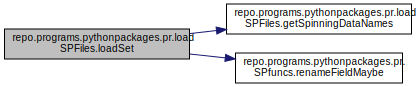
\includegraphics[width=350pt]{namespacerepo_1_1programs_1_1pythonpackages_1_1pr_1_1loadSPFiles_ac05316301b88456778eaedde597c8ed5_cgraph}
\end{center}
\end{figure}




Here is the caller graph for this function\-:
\nopagebreak
\begin{figure}[H]
\begin{center}
\leavevmode
\includegraphics[width=350pt]{namespacerepo_1_1programs_1_1pythonpackages_1_1pr_1_1loadSPFiles_ac05316301b88456778eaedde597c8ed5_icgraph}
\end{center}
\end{figure}


\hypertarget{namespacerepo_1_1programs_1_1pythonpackages_1_1pr_1_1loadSPFiles_a94905f8c986f1a826f5e14c6c271d3bc}{\index{repo\-::programs\-::pythonpackages\-::pr\-::load\-S\-P\-Files@{repo\-::programs\-::pythonpackages\-::pr\-::load\-S\-P\-Files}!load\-Set\-Info@{load\-Set\-Info}}
\index{load\-Set\-Info@{load\-Set\-Info}!repo::programs::pythonpackages::pr::loadSPFiles@{repo\-::programs\-::pythonpackages\-::pr\-::load\-S\-P\-Files}}
\subsubsection[{load\-Set\-Info}]{\setlength{\rightskip}{0pt plus 5cm}def repo.\-programs.\-pythonpackages.\-pr.\-load\-S\-P\-Files.\-load\-Set\-Info (
\begin{DoxyParamCaption}
\item[{}]{dir\-\_\-name}
\end{DoxyParamCaption}
)}}\label{namespacerepo_1_1programs_1_1pythonpackages_1_1pr_1_1loadSPFiles_a94905f8c986f1a826f5e14c6c271d3bc}


Definition at line 162 of file load\-S\-P\-Files.\-py.



Here is the call graph for this function\-:
\nopagebreak
\begin{figure}[H]
\begin{center}
\leavevmode
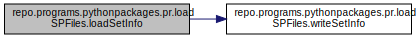
\includegraphics[width=350pt]{namespacerepo_1_1programs_1_1pythonpackages_1_1pr_1_1loadSPFiles_a94905f8c986f1a826f5e14c6c271d3bc_cgraph}
\end{center}
\end{figure}


\hypertarget{namespacerepo_1_1programs_1_1pythonpackages_1_1pr_1_1loadSPFiles_aa6876f5f9096cba233794dd03f719de3}{\index{repo\-::programs\-::pythonpackages\-::pr\-::load\-S\-P\-Files@{repo\-::programs\-::pythonpackages\-::pr\-::load\-S\-P\-Files}!load\-Zero\-File@{load\-Zero\-File}}
\index{load\-Zero\-File@{load\-Zero\-File}!repo::programs::pythonpackages::pr::loadSPFiles@{repo\-::programs\-::pythonpackages\-::pr\-::load\-S\-P\-Files}}
\subsubsection[{load\-Zero\-File}]{\setlength{\rightskip}{0pt plus 5cm}def repo.\-programs.\-pythonpackages.\-pr.\-load\-S\-P\-Files.\-load\-Zero\-File (
\begin{DoxyParamCaption}
\item[{}]{fname}
\end{DoxyParamCaption}
)}}\label{namespacerepo_1_1programs_1_1pythonpackages_1_1pr_1_1loadSPFiles_aa6876f5f9096cba233794dd03f719de3}


Definition at line 220 of file load\-S\-P\-Files.\-py.

\hypertarget{namespacerepo_1_1programs_1_1pythonpackages_1_1pr_1_1loadSPFiles_a7a17d807e31989fac9962e7eb5fa3de5}{\index{repo\-::programs\-::pythonpackages\-::pr\-::load\-S\-P\-Files@{repo\-::programs\-::pythonpackages\-::pr\-::load\-S\-P\-Files}!write\-Set\-Info@{write\-Set\-Info}}
\index{write\-Set\-Info@{write\-Set\-Info}!repo::programs::pythonpackages::pr::loadSPFiles@{repo\-::programs\-::pythonpackages\-::pr\-::load\-S\-P\-Files}}
\subsubsection[{write\-Set\-Info}]{\setlength{\rightskip}{0pt plus 5cm}def repo.\-programs.\-pythonpackages.\-pr.\-load\-S\-P\-Files.\-write\-Set\-Info (
\begin{DoxyParamCaption}
\item[{}]{dir\-\_\-name, }
\item[{}]{D}
\end{DoxyParamCaption}
)}}\label{namespacerepo_1_1programs_1_1pythonpackages_1_1pr_1_1loadSPFiles_a7a17d807e31989fac9962e7eb5fa3de5}


Definition at line 212 of file load\-S\-P\-Files.\-py.



Here is the caller graph for this function\-:
\nopagebreak
\begin{figure}[H]
\begin{center}
\leavevmode
\includegraphics[width=350pt]{namespacerepo_1_1programs_1_1pythonpackages_1_1pr_1_1loadSPFiles_a7a17d807e31989fac9962e7eb5fa3de5_icgraph}
\end{center}
\end{figure}




\subsection{Variable Documentation}
\hypertarget{namespacerepo_1_1programs_1_1pythonpackages_1_1pr_1_1loadSPFiles_a83183382a5277a75ee1031f6ef284691}{\index{repo\-::programs\-::pythonpackages\-::pr\-::load\-S\-P\-Files@{repo\-::programs\-::pythonpackages\-::pr\-::load\-S\-P\-Files}!dat@{dat}}
\index{dat@{dat}!repo::programs::pythonpackages::pr::loadSPFiles@{repo\-::programs\-::pythonpackages\-::pr\-::load\-S\-P\-Files}}
\subsubsection[{dat}]{\setlength{\rightskip}{0pt plus 5cm}tuple repo.\-programs.\-pythonpackages.\-pr.\-load\-S\-P\-Files.\-dat = {\bf load\-A\-Bin}({\bf fpath}, use\-Meta\-File=True)}}\label{namespacerepo_1_1programs_1_1pythonpackages_1_1pr_1_1loadSPFiles_a83183382a5277a75ee1031f6ef284691}


Definition at line 411 of file load\-S\-P\-Files.\-py.

\hypertarget{namespacerepo_1_1programs_1_1pythonpackages_1_1pr_1_1loadSPFiles_aed6d44730b91f4104569281ef51b335d}{\index{repo\-::programs\-::pythonpackages\-::pr\-::load\-S\-P\-Files@{repo\-::programs\-::pythonpackages\-::pr\-::load\-S\-P\-Files}!dat2@{dat2}}
\index{dat2@{dat2}!repo::programs::pythonpackages::pr::loadSPFiles@{repo\-::programs\-::pythonpackages\-::pr\-::load\-S\-P\-Files}}
\subsubsection[{dat2}]{\setlength{\rightskip}{0pt plus 5cm}tuple repo.\-programs.\-pythonpackages.\-pr.\-load\-S\-P\-Files.\-dat2 = {\bf load\-Bins}({\bf ddir}+'S\-P\-\_\-aparatus 5256.\-38 Medium')}}\label{namespacerepo_1_1programs_1_1pythonpackages_1_1pr_1_1loadSPFiles_aed6d44730b91f4104569281ef51b335d}


Definition at line 413 of file load\-S\-P\-Files.\-py.

\hypertarget{namespacerepo_1_1programs_1_1pythonpackages_1_1pr_1_1loadSPFiles_a450ab2273d44a0e76443c6e31b162908}{\index{repo\-::programs\-::pythonpackages\-::pr\-::load\-S\-P\-Files@{repo\-::programs\-::pythonpackages\-::pr\-::load\-S\-P\-Files}!dat3@{dat3}}
\index{dat3@{dat3}!repo::programs::pythonpackages::pr::loadSPFiles@{repo\-::programs\-::pythonpackages\-::pr\-::load\-S\-P\-Files}}
\subsubsection[{dat3}]{\setlength{\rightskip}{0pt plus 5cm}tuple repo.\-programs.\-pythonpackages.\-pr.\-load\-S\-P\-Files.\-dat3 = {\bf load\-Bins}({\bf ddir2}+{\bf fname2}, use\-Meta\-File=True)}}\label{namespacerepo_1_1programs_1_1pythonpackages_1_1pr_1_1loadSPFiles_a450ab2273d44a0e76443c6e31b162908}


Definition at line 414 of file load\-S\-P\-Files.\-py.

\hypertarget{namespacerepo_1_1programs_1_1pythonpackages_1_1pr_1_1loadSPFiles_a8966ac451acc4e186f9a8c9d299da497}{\index{repo\-::programs\-::pythonpackages\-::pr\-::load\-S\-P\-Files@{repo\-::programs\-::pythonpackages\-::pr\-::load\-S\-P\-Files}!dat\-\_\-f@{dat\-\_\-f}}
\index{dat\-\_\-f@{dat\-\_\-f}!repo::programs::pythonpackages::pr::loadSPFiles@{repo\-::programs\-::pythonpackages\-::pr\-::load\-S\-P\-Files}}
\subsubsection[{dat\-\_\-f}]{\setlength{\rightskip}{0pt plus 5cm}tuple repo.\-programs.\-pythonpackages.\-pr.\-load\-S\-P\-Files.\-dat\-\_\-f = {\bf load\-Bins}({\bf fpath\-\_\-f}, use\-Meta\-File=False, total\-Data\-Type=\mbox{[}('sd','$>$f8'), ('s1', '$>$f4')\mbox{]})}}\label{namespacerepo_1_1programs_1_1pythonpackages_1_1pr_1_1loadSPFiles_a8966ac451acc4e186f9a8c9d299da497}


Definition at line 412 of file load\-S\-P\-Files.\-py.

\hypertarget{namespacerepo_1_1programs_1_1pythonpackages_1_1pr_1_1loadSPFiles_a65abcc2d7333a2e99d3d3376b616f959}{\index{repo\-::programs\-::pythonpackages\-::pr\-::load\-S\-P\-Files@{repo\-::programs\-::pythonpackages\-::pr\-::load\-S\-P\-Files}!ddir@{ddir}}
\index{ddir@{ddir}!repo::programs::pythonpackages::pr::loadSPFiles@{repo\-::programs\-::pythonpackages\-::pr\-::load\-S\-P\-Files}}
\subsubsection[{ddir}]{\setlength{\rightskip}{0pt plus 5cm}string repo.\-programs.\-pythonpackages.\-pr.\-load\-S\-P\-Files.\-ddir = '/media/morgan/6a0066c2-\/6c13-\/49f4-\/9322-\/0b818dda2fe8/\-Princeton Data/\-South Pole/\-S\-P\-\_\-aparatus 5256.\-38 Bundle/'}}\label{namespacerepo_1_1programs_1_1pythonpackages_1_1pr_1_1loadSPFiles_a65abcc2d7333a2e99d3d3376b616f959}


Definition at line 402 of file load\-S\-P\-Files.\-py.

\hypertarget{namespacerepo_1_1programs_1_1pythonpackages_1_1pr_1_1loadSPFiles_a39efcdddf61ee790cdf9c4dfbd9e7080}{\index{repo\-::programs\-::pythonpackages\-::pr\-::load\-S\-P\-Files@{repo\-::programs\-::pythonpackages\-::pr\-::load\-S\-P\-Files}!ddir2@{ddir2}}
\index{ddir2@{ddir2}!repo::programs::pythonpackages::pr::loadSPFiles@{repo\-::programs\-::pythonpackages\-::pr\-::load\-S\-P\-Files}}
\subsubsection[{ddir2}]{\setlength{\rightskip}{0pt plus 5cm}string repo.\-programs.\-pythonpackages.\-pr.\-load\-S\-P\-Files.\-ddir2 = '/media/morgan/6a0066c2-\/6c13-\/49f4-\/9322-\/0b818dda2fe8/\-Princeton Data/\-South Pole/\-S\-P\-\_\-motor 5253.\-67 Bundle/'}}\label{namespacerepo_1_1programs_1_1pythonpackages_1_1pr_1_1loadSPFiles_a39efcdddf61ee790cdf9c4dfbd9e7080}


Definition at line 406 of file load\-S\-P\-Files.\-py.

\hypertarget{namespacerepo_1_1programs_1_1pythonpackages_1_1pr_1_1loadSPFiles_acfe87f91d2373c3c41bf59a6024b8a94}{\index{repo\-::programs\-::pythonpackages\-::pr\-::load\-S\-P\-Files@{repo\-::programs\-::pythonpackages\-::pr\-::load\-S\-P\-Files}!fname@{fname}}
\index{fname@{fname}!repo::programs::pythonpackages::pr::loadSPFiles@{repo\-::programs\-::pythonpackages\-::pr\-::load\-S\-P\-Files}}
\subsubsection[{fname}]{\setlength{\rightskip}{0pt plus 5cm}string repo.\-programs.\-pythonpackages.\-pr.\-load\-S\-P\-Files.\-fname = 'S\-P\-\_\-aparatus 5256.\-38 Medium 6.bin'}}\label{namespacerepo_1_1programs_1_1pythonpackages_1_1pr_1_1loadSPFiles_acfe87f91d2373c3c41bf59a6024b8a94}


Definition at line 404 of file load\-S\-P\-Files.\-py.

\hypertarget{namespacerepo_1_1programs_1_1pythonpackages_1_1pr_1_1loadSPFiles_a9058f0ead0c926f493bb7f6ae52a49ea}{\index{repo\-::programs\-::pythonpackages\-::pr\-::load\-S\-P\-Files@{repo\-::programs\-::pythonpackages\-::pr\-::load\-S\-P\-Files}!fname2@{fname2}}
\index{fname2@{fname2}!repo::programs::pythonpackages::pr::loadSPFiles@{repo\-::programs\-::pythonpackages\-::pr\-::load\-S\-P\-Files}}
\subsubsection[{fname2}]{\setlength{\rightskip}{0pt plus 5cm}string repo.\-programs.\-pythonpackages.\-pr.\-load\-S\-P\-Files.\-fname2 = 'S\-P\-\_\-motor 5253.\-67 sensors'}}\label{namespacerepo_1_1programs_1_1pythonpackages_1_1pr_1_1loadSPFiles_a9058f0ead0c926f493bb7f6ae52a49ea}


Definition at line 407 of file load\-S\-P\-Files.\-py.

\hypertarget{namespacerepo_1_1programs_1_1pythonpackages_1_1pr_1_1loadSPFiles_af897386d87d4d72567fb337653aa3105}{\index{repo\-::programs\-::pythonpackages\-::pr\-::load\-S\-P\-Files@{repo\-::programs\-::pythonpackages\-::pr\-::load\-S\-P\-Files}!fname\-\_\-f@{fname\-\_\-f}}
\index{fname\-\_\-f@{fname\-\_\-f}!repo::programs::pythonpackages::pr::loadSPFiles@{repo\-::programs\-::pythonpackages\-::pr\-::load\-S\-P\-Files}}
\subsubsection[{fname\-\_\-f}]{\setlength{\rightskip}{0pt plus 5cm}string repo.\-programs.\-pythonpackages.\-pr.\-load\-S\-P\-Files.\-fname\-\_\-f = 'S\-P\-\_\-aparatus 5256.\-38 Fast'}}\label{namespacerepo_1_1programs_1_1pythonpackages_1_1pr_1_1loadSPFiles_af897386d87d4d72567fb337653aa3105}


Definition at line 405 of file load\-S\-P\-Files.\-py.

\hypertarget{namespacerepo_1_1programs_1_1pythonpackages_1_1pr_1_1loadSPFiles_a8ffbf3fed92bc26b4248caebb30ade38}{\index{repo\-::programs\-::pythonpackages\-::pr\-::load\-S\-P\-Files@{repo\-::programs\-::pythonpackages\-::pr\-::load\-S\-P\-Files}!fpath@{fpath}}
\index{fpath@{fpath}!repo::programs::pythonpackages::pr::loadSPFiles@{repo\-::programs\-::pythonpackages\-::pr\-::load\-S\-P\-Files}}
\subsubsection[{fpath}]{\setlength{\rightskip}{0pt plus 5cm}repo.\-programs.\-pythonpackages.\-pr.\-load\-S\-P\-Files.\-fpath = {\bf ddir}+{\bf fname}}}\label{namespacerepo_1_1programs_1_1pythonpackages_1_1pr_1_1loadSPFiles_a8ffbf3fed92bc26b4248caebb30ade38}


Definition at line 408 of file load\-S\-P\-Files.\-py.

\hypertarget{namespacerepo_1_1programs_1_1pythonpackages_1_1pr_1_1loadSPFiles_a931d7ee8b1015ac25cbca6eee1f77bea}{\index{repo\-::programs\-::pythonpackages\-::pr\-::load\-S\-P\-Files@{repo\-::programs\-::pythonpackages\-::pr\-::load\-S\-P\-Files}!fpath\-\_\-f@{fpath\-\_\-f}}
\index{fpath\-\_\-f@{fpath\-\_\-f}!repo::programs::pythonpackages::pr::loadSPFiles@{repo\-::programs\-::pythonpackages\-::pr\-::load\-S\-P\-Files}}
\subsubsection[{fpath\-\_\-f}]{\setlength{\rightskip}{0pt plus 5cm}repo.\-programs.\-pythonpackages.\-pr.\-load\-S\-P\-Files.\-fpath\-\_\-f = {\bf ddir}+{\bf fname\-\_\-f}}}\label{namespacerepo_1_1programs_1_1pythonpackages_1_1pr_1_1loadSPFiles_a931d7ee8b1015ac25cbca6eee1f77bea}


Definition at line 409 of file load\-S\-P\-Files.\-py.

\hypertarget{namespacerepo_1_1programs_1_1pythonpackages_1_1pr_1_1loadSPFiles_af4aa2bb0015793d7b7e493e4aa4f4b8c}{\index{repo\-::programs\-::pythonpackages\-::pr\-::load\-S\-P\-Files@{repo\-::programs\-::pythonpackages\-::pr\-::load\-S\-P\-Files}!medium\-Names@{medium\-Names}}
\index{medium\-Names@{medium\-Names}!repo::programs::pythonpackages::pr::loadSPFiles@{repo\-::programs\-::pythonpackages\-::pr\-::load\-S\-P\-Files}}
\subsubsection[{medium\-Names}]{\setlength{\rightskip}{0pt plus 5cm}string repo.\-programs.\-pythonpackages.\-pr.\-load\-S\-P\-Files.\-medium\-Names}}\label{namespacerepo_1_1programs_1_1pythonpackages_1_1pr_1_1loadSPFiles_af4aa2bb0015793d7b7e493e4aa4f4b8c}
{\bfseries Initial value\-:}
\begin{DoxyCode}
1 = \textcolor{stringliteral}{"""Accelerometer}
2 \textcolor{stringliteral}{Position Purple}
3 \textcolor{stringliteral}{Position Green}
4 \textcolor{stringliteral}{Fluxgate X}
5 \textcolor{stringliteral}{Fluxgate Y}
6 \textcolor{stringliteral}{Fluxgate Z}
7 \textcolor{stringliteral}{Tiltmeter X}
8 \textcolor{stringliteral}{Tiltmeter Y}
9 \textcolor{stringliteral}{Vert Pos Det}
10 \textcolor{stringliteral}{Horiz Pos Det}
11 \textcolor{stringliteral}{Vert Pos Det 2}
12 \textcolor{stringliteral}{Horiz Pos Det 2}
13 \textcolor{stringliteral}{Vert Pos Det 3}
14 \textcolor{stringliteral}{Horiz Pos Det 3}
15 \textcolor{stringliteral}{"""}
\end{DoxyCode}


Definition at line 34 of file load\-S\-P\-Files.\-py.

\hypertarget{namespacerepo_1_1programs_1_1pythonpackages_1_1pr_1_1loadSPFiles_a92ba966a3b7423fd4d0c7874d3f92e71}{\index{repo\-::programs\-::pythonpackages\-::pr\-::load\-S\-P\-Files@{repo\-::programs\-::pythonpackages\-::pr\-::load\-S\-P\-Files}!relaxed\-Names@{relaxed\-Names}}
\index{relaxed\-Names@{relaxed\-Names}!repo::programs::pythonpackages::pr::loadSPFiles@{repo\-::programs\-::pythonpackages\-::pr\-::load\-S\-P\-Files}}
\subsubsection[{relaxed\-Names}]{\setlength{\rightskip}{0pt plus 5cm}string repo.\-programs.\-pythonpackages.\-pr.\-load\-S\-P\-Files.\-relaxed\-Names}}\label{namespacerepo_1_1programs_1_1pythonpackages_1_1pr_1_1loadSPFiles_a92ba966a3b7423fd4d0c7874d3f92e71}
{\bfseries Initial value\-:}
\begin{DoxyCode}
1 = \textcolor{stringliteral}{"""Tot Pos Det}
2 \textcolor{stringliteral}{Tot Pos Det 2}
3 \textcolor{stringliteral}{Tot Pos Det 3}
4 \textcolor{stringliteral}{Cell Temp}
5 \textcolor{stringliteral}{Ferrite Temp}
6 \textcolor{stringliteral}{Oven Temp}
7 \textcolor{stringliteral}{Temperature Controller Output}
8 \textcolor{stringliteral}{Breadboard Temp}
9 \textcolor{stringliteral}{Room Temp}
10 \textcolor{stringliteral}{G10 Lid Temp}
11 \textcolor{stringliteral}{Tilt Sensor 1}
12 \textcolor{stringliteral}{Tilt Sensor 2}
13 \textcolor{stringliteral}{WavelengthErr}
14 \textcolor{stringliteral}{Pump Current Mon}
15 \textcolor{stringliteral}{Pump Temp Mon}
16 \textcolor{stringliteral}{Probe Current Mon}
17 \textcolor{stringliteral}{Probe Temp Mon}
18 \textcolor{stringliteral}{Water Flow}
19 \textcolor{stringliteral}{Apparatus Position}
20 \textcolor{stringliteral}{"""}
\end{DoxyCode}


Definition at line 14 of file load\-S\-P\-Files.\-py.


\hypertarget{namespacerepo_1_1programs_1_1pythonpackages_1_1pr_1_1openCPT}{\section{repo.\-programs.\-pythonpackages.\-pr.\-open\-C\-P\-T Namespace Reference}
\label{namespacerepo_1_1programs_1_1pythonpackages_1_1pr_1_1openCPT}\index{repo.\-programs.\-pythonpackages.\-pr.\-open\-C\-P\-T@{repo.\-programs.\-pythonpackages.\-pr.\-open\-C\-P\-T}}
}
\subsection*{Functions}
\begin{DoxyCompactItemize}
\item 
def \hyperlink{namespacerepo_1_1programs_1_1pythonpackages_1_1pr_1_1openCPT_a8d2cf2d1cdb625fa3ea7d0ec4e7af575}{load\-Apparatus\-Files}
\item 
def \hyperlink{namespacerepo_1_1programs_1_1pythonpackages_1_1pr_1_1openCPT_a123c419a688aefb0d6d482eca7512d36}{open\-File}
\end{DoxyCompactItemize}
\subsection*{Variables}
\begin{DoxyCompactItemize}
\item 
list \hyperlink{namespacerepo_1_1programs_1_1pythonpackages_1_1pr_1_1openCPT_a6195f6525b22b29221384f9235fe1062}{base\-\_\-dir} = os.\-environ\mbox{[}'S\-P\-\_\-\-D\-A\-T\-A\-\_\-\-D\-I\-R'\mbox{]}
\item 
string \hyperlink{namespacerepo_1_1programs_1_1pythonpackages_1_1pr_1_1openCPT_a629d9addea1bbee10544941d7c301ba8}{ddir} = \char`\"{}/media/morgan/6a0066c2-\/6c13-\/49f4-\/9322-\/0b818dda2fe8/\-Princeton Data/\-South Pole/\-S\-P\-\_\-aparatus 5240.\-33 Bundle/\char`\"{}
\item 
string \hyperlink{namespacerepo_1_1programs_1_1pythonpackages_1_1pr_1_1openCPT_ad49f00cb69a927479558926f2158898f}{filepath} = \hyperlink{namespacerepo_1_1programs_1_1pythonpackages_1_1pr_1_1openCPT_a629d9addea1bbee10544941d7c301ba8}{ddir}+\char`\"{}S\-P\-\_\-aparatus 5240.\-33 Medium 2.bin\char`\"{}
\item 
string \hyperlink{namespacerepo_1_1programs_1_1pythonpackages_1_1pr_1_1openCPT_a87910852db48cafc314ea9372f00a401}{template\-\_\-regex} = 'S\-P\-\_\-aparatus (\textbackslash{}d+(?\-:\textbackslash{}.\textbackslash{}d$\ast$)?$\vert$\textbackslash{}.\textbackslash{}d+) \{0\}( \textbackslash{}d+)?\textbackslash{}.bin'
\item 
tuple \hyperlink{namespacerepo_1_1programs_1_1pythonpackages_1_1pr_1_1openCPT_a3e5077d300b3260fd9aa1487e0e15a3e}{dat} = \hyperlink{namespacerepo_1_1programs_1_1pythonpackages_1_1pr_1_1openCPT_a8d2cf2d1cdb625fa3ea7d0ec4e7af575}{load\-Apparatus\-Files}(\hyperlink{namespacerepo_1_1programs_1_1pythonpackages_1_1pr_1_1openCPT_a629d9addea1bbee10544941d7c301ba8}{ddir}+'S\-P\-\_\-aparatus 5240.\-33 Medium')
\end{DoxyCompactItemize}


\subsection{Function Documentation}
\hypertarget{namespacerepo_1_1programs_1_1pythonpackages_1_1pr_1_1openCPT_a8d2cf2d1cdb625fa3ea7d0ec4e7af575}{\index{repo\-::programs\-::pythonpackages\-::pr\-::open\-C\-P\-T@{repo\-::programs\-::pythonpackages\-::pr\-::open\-C\-P\-T}!load\-Apparatus\-Files@{load\-Apparatus\-Files}}
\index{load\-Apparatus\-Files@{load\-Apparatus\-Files}!repo::programs::pythonpackages::pr::openCPT@{repo\-::programs\-::pythonpackages\-::pr\-::open\-C\-P\-T}}
\subsubsection[{load\-Apparatus\-Files}]{\setlength{\rightskip}{0pt plus 5cm}def repo.\-programs.\-pythonpackages.\-pr.\-open\-C\-P\-T.\-load\-Apparatus\-Files (
\begin{DoxyParamCaption}
\item[{}]{root\-\_\-path, }
\item[{}]{use\-Meta\-File = {\ttfamily True}}
\end{DoxyParamCaption}
)}}\label{namespacerepo_1_1programs_1_1pythonpackages_1_1pr_1_1openCPT_a8d2cf2d1cdb625fa3ea7d0ec4e7af575}


Definition at line 13 of file open\-C\-P\-T.\-py.



Here is the call graph for this function\-:
\nopagebreak
\begin{figure}[H]
\begin{center}
\leavevmode
\includegraphics[width=350pt]{namespacerepo_1_1programs_1_1pythonpackages_1_1pr_1_1openCPT_a8d2cf2d1cdb625fa3ea7d0ec4e7af575_cgraph}
\end{center}
\end{figure}


\hypertarget{namespacerepo_1_1programs_1_1pythonpackages_1_1pr_1_1openCPT_a123c419a688aefb0d6d482eca7512d36}{\index{repo\-::programs\-::pythonpackages\-::pr\-::open\-C\-P\-T@{repo\-::programs\-::pythonpackages\-::pr\-::open\-C\-P\-T}!open\-File@{open\-File}}
\index{open\-File@{open\-File}!repo::programs::pythonpackages::pr::openCPT@{repo\-::programs\-::pythonpackages\-::pr\-::open\-C\-P\-T}}
\subsubsection[{open\-File}]{\setlength{\rightskip}{0pt plus 5cm}def repo.\-programs.\-pythonpackages.\-pr.\-open\-C\-P\-T.\-open\-File (
\begin{DoxyParamCaption}
\item[{}]{filepath, }
\item[{}]{n\-Vars = {\ttfamily 1}, }
\item[{}]{use\-Meta\-File = {\ttfamily False}, }
\item[{}]{endian = {\ttfamily '$>$'}}
\end{DoxyParamCaption}
)}}\label{namespacerepo_1_1programs_1_1pythonpackages_1_1pr_1_1openCPT_a123c419a688aefb0d6d482eca7512d36}


Definition at line 28 of file open\-C\-P\-T.\-py.



Here is the caller graph for this function\-:
\nopagebreak
\begin{figure}[H]
\begin{center}
\leavevmode
\includegraphics[width=350pt]{namespacerepo_1_1programs_1_1pythonpackages_1_1pr_1_1openCPT_a123c419a688aefb0d6d482eca7512d36_icgraph}
\end{center}
\end{figure}




\subsection{Variable Documentation}
\hypertarget{namespacerepo_1_1programs_1_1pythonpackages_1_1pr_1_1openCPT_a6195f6525b22b29221384f9235fe1062}{\index{repo\-::programs\-::pythonpackages\-::pr\-::open\-C\-P\-T@{repo\-::programs\-::pythonpackages\-::pr\-::open\-C\-P\-T}!base\-\_\-dir@{base\-\_\-dir}}
\index{base\-\_\-dir@{base\-\_\-dir}!repo::programs::pythonpackages::pr::openCPT@{repo\-::programs\-::pythonpackages\-::pr\-::open\-C\-P\-T}}
\subsubsection[{base\-\_\-dir}]{\setlength{\rightskip}{0pt plus 5cm}list repo.\-programs.\-pythonpackages.\-pr.\-open\-C\-P\-T.\-base\-\_\-dir = os.\-environ\mbox{[}'S\-P\-\_\-\-D\-A\-T\-A\-\_\-\-D\-I\-R'\mbox{]}}}\label{namespacerepo_1_1programs_1_1pythonpackages_1_1pr_1_1openCPT_a6195f6525b22b29221384f9235fe1062}


Definition at line 6 of file open\-C\-P\-T.\-py.

\hypertarget{namespacerepo_1_1programs_1_1pythonpackages_1_1pr_1_1openCPT_a3e5077d300b3260fd9aa1487e0e15a3e}{\index{repo\-::programs\-::pythonpackages\-::pr\-::open\-C\-P\-T@{repo\-::programs\-::pythonpackages\-::pr\-::open\-C\-P\-T}!dat@{dat}}
\index{dat@{dat}!repo::programs::pythonpackages::pr::openCPT@{repo\-::programs\-::pythonpackages\-::pr\-::open\-C\-P\-T}}
\subsubsection[{dat}]{\setlength{\rightskip}{0pt plus 5cm}tuple repo.\-programs.\-pythonpackages.\-pr.\-open\-C\-P\-T.\-dat = {\bf load\-Apparatus\-Files}({\bf ddir}+'S\-P\-\_\-aparatus 5240.\-33 Medium')}}\label{namespacerepo_1_1programs_1_1pythonpackages_1_1pr_1_1openCPT_a3e5077d300b3260fd9aa1487e0e15a3e}


Definition at line 63 of file open\-C\-P\-T.\-py.

\hypertarget{namespacerepo_1_1programs_1_1pythonpackages_1_1pr_1_1openCPT_a629d9addea1bbee10544941d7c301ba8}{\index{repo\-::programs\-::pythonpackages\-::pr\-::open\-C\-P\-T@{repo\-::programs\-::pythonpackages\-::pr\-::open\-C\-P\-T}!ddir@{ddir}}
\index{ddir@{ddir}!repo::programs::pythonpackages::pr::openCPT@{repo\-::programs\-::pythonpackages\-::pr\-::open\-C\-P\-T}}
\subsubsection[{ddir}]{\setlength{\rightskip}{0pt plus 5cm}string repo.\-programs.\-pythonpackages.\-pr.\-open\-C\-P\-T.\-ddir = \char`\"{}/media/morgan/6a0066c2-\/6c13-\/49f4-\/9322-\/0b818dda2fe8/\-Princeton Data/\-South Pole/\-S\-P\-\_\-aparatus 5240.\-33 Bundle/\char`\"{}}}\label{namespacerepo_1_1programs_1_1pythonpackages_1_1pr_1_1openCPT_a629d9addea1bbee10544941d7c301ba8}


Definition at line 7 of file open\-C\-P\-T.\-py.

\hypertarget{namespacerepo_1_1programs_1_1pythonpackages_1_1pr_1_1openCPT_ad49f00cb69a927479558926f2158898f}{\index{repo\-::programs\-::pythonpackages\-::pr\-::open\-C\-P\-T@{repo\-::programs\-::pythonpackages\-::pr\-::open\-C\-P\-T}!filepath@{filepath}}
\index{filepath@{filepath}!repo::programs::pythonpackages::pr::openCPT@{repo\-::programs\-::pythonpackages\-::pr\-::open\-C\-P\-T}}
\subsubsection[{filepath}]{\setlength{\rightskip}{0pt plus 5cm}string repo.\-programs.\-pythonpackages.\-pr.\-open\-C\-P\-T.\-filepath = {\bf ddir}+\char`\"{}S\-P\-\_\-aparatus 5240.\-33 Medium 2.bin\char`\"{}}}\label{namespacerepo_1_1programs_1_1pythonpackages_1_1pr_1_1openCPT_ad49f00cb69a927479558926f2158898f}


Definition at line 8 of file open\-C\-P\-T.\-py.

\hypertarget{namespacerepo_1_1programs_1_1pythonpackages_1_1pr_1_1openCPT_a87910852db48cafc314ea9372f00a401}{\index{repo\-::programs\-::pythonpackages\-::pr\-::open\-C\-P\-T@{repo\-::programs\-::pythonpackages\-::pr\-::open\-C\-P\-T}!template\-\_\-regex@{template\-\_\-regex}}
\index{template\-\_\-regex@{template\-\_\-regex}!repo::programs::pythonpackages::pr::openCPT@{repo\-::programs\-::pythonpackages\-::pr\-::open\-C\-P\-T}}
\subsubsection[{template\-\_\-regex}]{\setlength{\rightskip}{0pt plus 5cm}string repo.\-programs.\-pythonpackages.\-pr.\-open\-C\-P\-T.\-template\-\_\-regex = 'S\-P\-\_\-aparatus (\textbackslash{}d+(?\-:\textbackslash{}.\textbackslash{}d$\ast$)?$\vert$\textbackslash{}.\textbackslash{}d+) \{0\}( \textbackslash{}d+)?\textbackslash{}.bin'}}\label{namespacerepo_1_1programs_1_1pythonpackages_1_1pr_1_1openCPT_a87910852db48cafc314ea9372f00a401}


Definition at line 11 of file open\-C\-P\-T.\-py.


\hypertarget{namespacerepo_1_1programs_1_1pythonpackages_1_1pr_1_1openMotor}{\section{repo.\-programs.\-pythonpackages.\-pr.\-open\-Motor Namespace Reference}
\label{namespacerepo_1_1programs_1_1pythonpackages_1_1pr_1_1openMotor}\index{repo.\-programs.\-pythonpackages.\-pr.\-open\-Motor@{repo.\-programs.\-pythonpackages.\-pr.\-open\-Motor}}
}
\subsection*{Functions}
\begin{DoxyCompactItemize}
\item 
def \hyperlink{namespacerepo_1_1programs_1_1pythonpackages_1_1pr_1_1openMotor_a67f554beaac0864d301fab58bf86397b}{load\-Bins}
\item 
def \hyperlink{namespacerepo_1_1programs_1_1pythonpackages_1_1pr_1_1openMotor_a04420d495757844bca7113b696a2cb1d}{load\-Abin}
\end{DoxyCompactItemize}
\subsection*{Variables}
\begin{DoxyCompactItemize}
\item 
string \hyperlink{namespacerepo_1_1programs_1_1pythonpackages_1_1pr_1_1openMotor_ab3fcb2684f3321af9bd6715fa1c12675}{ddir} = '/media/morgan/6a0066c2-\/6c13-\/49f4-\/9322-\/0b818dda2fe8/\-Princeton Data/\-South Pole/\-S\-P\-\_\-aparatus 5256.\-38 Bundle/'
\item 
string \hyperlink{namespacerepo_1_1programs_1_1pythonpackages_1_1pr_1_1openMotor_a1ca6afbef052898575edbdf81a19cce4}{fname} = 'S\-P\-\_\-aparatus 5256.\-38 Medium 6.bin'
\item 
string \hyperlink{namespacerepo_1_1programs_1_1pythonpackages_1_1pr_1_1openMotor_a7845f46665131b51ba25ba3adfaf4958}{ddir2} = '/media/morgan/6a0066c2-\/6c13-\/49f4-\/9322-\/0b818dda2fe8/\-Princeton Data/\-South Pole/\-S\-P\-\_\-motor 5253.\-67 Bundle/'
\item 
string \hyperlink{namespacerepo_1_1programs_1_1pythonpackages_1_1pr_1_1openMotor_ab3194f8b875a45048365db97cf0d0fd0}{fname2} = 'S\-P\-\_\-motor 5253.\-67 sensors'
\item 
\hyperlink{namespacerepo_1_1programs_1_1pythonpackages_1_1pr_1_1openMotor_aa622e663d644f1b366ed96d4f2b34cf2}{fpath} = \hyperlink{namespacerepo_1_1programs_1_1pythonpackages_1_1pr_1_1openMotor_ab3fcb2684f3321af9bd6715fa1c12675}{ddir}+\hyperlink{namespacerepo_1_1programs_1_1pythonpackages_1_1pr_1_1openMotor_a1ca6afbef052898575edbdf81a19cce4}{fname}
\item 
tuple \hyperlink{namespacerepo_1_1programs_1_1pythonpackages_1_1pr_1_1openMotor_aba6f1fba127e2142e12df0163a37f98c}{dat} = \hyperlink{namespacerepo_1_1programs_1_1pythonpackages_1_1pr_1_1openMotor_a04420d495757844bca7113b696a2cb1d}{load\-Abin}(\hyperlink{namespacerepo_1_1programs_1_1pythonpackages_1_1pr_1_1openMotor_aa622e663d644f1b366ed96d4f2b34cf2}{fpath}, use\-Meta\-File=True)
\item 
tuple \hyperlink{namespacerepo_1_1programs_1_1pythonpackages_1_1pr_1_1openMotor_a7e71c31c6f2be1f7dd4c5818fbc3b12e}{dat2} = \hyperlink{namespacerepo_1_1programs_1_1pythonpackages_1_1pr_1_1openMotor_a67f554beaac0864d301fab58bf86397b}{load\-Bins}(\hyperlink{namespacerepo_1_1programs_1_1pythonpackages_1_1pr_1_1openMotor_ab3fcb2684f3321af9bd6715fa1c12675}{ddir}+'S\-P\-\_\-aparatus 5256.\-38 Medium')
\item 
tuple \hyperlink{namespacerepo_1_1programs_1_1pythonpackages_1_1pr_1_1openMotor_a7e9dd8e353fa85c7c0ecdda03da8d64e}{dat3} = \hyperlink{namespacerepo_1_1programs_1_1pythonpackages_1_1pr_1_1openMotor_a67f554beaac0864d301fab58bf86397b}{load\-Bins}(\hyperlink{namespacerepo_1_1programs_1_1pythonpackages_1_1pr_1_1openMotor_a7845f46665131b51ba25ba3adfaf4958}{ddir2}+\hyperlink{namespacerepo_1_1programs_1_1pythonpackages_1_1pr_1_1openMotor_ab3194f8b875a45048365db97cf0d0fd0}{fname2}, use\-Meta\-File=True)
\end{DoxyCompactItemize}


\subsection{Function Documentation}
\hypertarget{namespacerepo_1_1programs_1_1pythonpackages_1_1pr_1_1openMotor_a04420d495757844bca7113b696a2cb1d}{\index{repo\-::programs\-::pythonpackages\-::pr\-::open\-Motor@{repo\-::programs\-::pythonpackages\-::pr\-::open\-Motor}!load\-Abin@{load\-Abin}}
\index{load\-Abin@{load\-Abin}!repo::programs::pythonpackages::pr::openMotor@{repo\-::programs\-::pythonpackages\-::pr\-::open\-Motor}}
\subsubsection[{load\-Abin}]{\setlength{\rightskip}{0pt plus 5cm}def repo.\-programs.\-pythonpackages.\-pr.\-open\-Motor.\-load\-Abin (
\begin{DoxyParamCaption}
\item[{}]{filepath, }
\item[{}]{n\-Vars = {\ttfamily 1}, }
\item[{}]{use\-Meta\-File = {\ttfamily True}, }
\item[{}]{endian = {\ttfamily ''}}
\end{DoxyParamCaption}
)}}\label{namespacerepo_1_1programs_1_1pythonpackages_1_1pr_1_1openMotor_a04420d495757844bca7113b696a2cb1d}


Definition at line 24 of file open\-Motor.\-py.



Here is the caller graph for this function\-:
\nopagebreak
\begin{figure}[H]
\begin{center}
\leavevmode
\includegraphics[width=350pt]{namespacerepo_1_1programs_1_1pythonpackages_1_1pr_1_1openMotor_a04420d495757844bca7113b696a2cb1d_icgraph}
\end{center}
\end{figure}


\hypertarget{namespacerepo_1_1programs_1_1pythonpackages_1_1pr_1_1openMotor_a67f554beaac0864d301fab58bf86397b}{\index{repo\-::programs\-::pythonpackages\-::pr\-::open\-Motor@{repo\-::programs\-::pythonpackages\-::pr\-::open\-Motor}!load\-Bins@{load\-Bins}}
\index{load\-Bins@{load\-Bins}!repo::programs::pythonpackages::pr::openMotor@{repo\-::programs\-::pythonpackages\-::pr\-::open\-Motor}}
\subsubsection[{load\-Bins}]{\setlength{\rightskip}{0pt plus 5cm}def repo.\-programs.\-pythonpackages.\-pr.\-open\-Motor.\-load\-Bins (
\begin{DoxyParamCaption}
\item[{}]{root\-\_\-path, }
\item[{}]{use\-Meta\-File = {\ttfamily True}}
\end{DoxyParamCaption}
)}}\label{namespacerepo_1_1programs_1_1pythonpackages_1_1pr_1_1openMotor_a67f554beaac0864d301fab58bf86397b}


Definition at line 7 of file open\-Motor.\-py.



Here is the call graph for this function\-:
\nopagebreak
\begin{figure}[H]
\begin{center}
\leavevmode
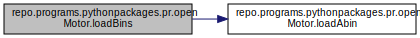
\includegraphics[width=350pt]{namespacerepo_1_1programs_1_1pythonpackages_1_1pr_1_1openMotor_a67f554beaac0864d301fab58bf86397b_cgraph}
\end{center}
\end{figure}




\subsection{Variable Documentation}
\hypertarget{namespacerepo_1_1programs_1_1pythonpackages_1_1pr_1_1openMotor_aba6f1fba127e2142e12df0163a37f98c}{\index{repo\-::programs\-::pythonpackages\-::pr\-::open\-Motor@{repo\-::programs\-::pythonpackages\-::pr\-::open\-Motor}!dat@{dat}}
\index{dat@{dat}!repo::programs::pythonpackages::pr::openMotor@{repo\-::programs\-::pythonpackages\-::pr\-::open\-Motor}}
\subsubsection[{dat}]{\setlength{\rightskip}{0pt plus 5cm}tuple repo.\-programs.\-pythonpackages.\-pr.\-open\-Motor.\-dat = {\bf load\-Abin}({\bf fpath}, use\-Meta\-File=True)}}\label{namespacerepo_1_1programs_1_1pythonpackages_1_1pr_1_1openMotor_aba6f1fba127e2142e12df0163a37f98c}


Definition at line 88 of file open\-Motor.\-py.

\hypertarget{namespacerepo_1_1programs_1_1pythonpackages_1_1pr_1_1openMotor_a7e71c31c6f2be1f7dd4c5818fbc3b12e}{\index{repo\-::programs\-::pythonpackages\-::pr\-::open\-Motor@{repo\-::programs\-::pythonpackages\-::pr\-::open\-Motor}!dat2@{dat2}}
\index{dat2@{dat2}!repo::programs::pythonpackages::pr::openMotor@{repo\-::programs\-::pythonpackages\-::pr\-::open\-Motor}}
\subsubsection[{dat2}]{\setlength{\rightskip}{0pt plus 5cm}tuple repo.\-programs.\-pythonpackages.\-pr.\-open\-Motor.\-dat2 = {\bf load\-Bins}({\bf ddir}+'S\-P\-\_\-aparatus 5256.\-38 Medium')}}\label{namespacerepo_1_1programs_1_1pythonpackages_1_1pr_1_1openMotor_a7e71c31c6f2be1f7dd4c5818fbc3b12e}


Definition at line 89 of file open\-Motor.\-py.

\hypertarget{namespacerepo_1_1programs_1_1pythonpackages_1_1pr_1_1openMotor_a7e9dd8e353fa85c7c0ecdda03da8d64e}{\index{repo\-::programs\-::pythonpackages\-::pr\-::open\-Motor@{repo\-::programs\-::pythonpackages\-::pr\-::open\-Motor}!dat3@{dat3}}
\index{dat3@{dat3}!repo::programs::pythonpackages::pr::openMotor@{repo\-::programs\-::pythonpackages\-::pr\-::open\-Motor}}
\subsubsection[{dat3}]{\setlength{\rightskip}{0pt plus 5cm}tuple repo.\-programs.\-pythonpackages.\-pr.\-open\-Motor.\-dat3 = {\bf load\-Bins}({\bf ddir2}+{\bf fname2}, use\-Meta\-File=True)}}\label{namespacerepo_1_1programs_1_1pythonpackages_1_1pr_1_1openMotor_a7e9dd8e353fa85c7c0ecdda03da8d64e}


Definition at line 90 of file open\-Motor.\-py.

\hypertarget{namespacerepo_1_1programs_1_1pythonpackages_1_1pr_1_1openMotor_ab3fcb2684f3321af9bd6715fa1c12675}{\index{repo\-::programs\-::pythonpackages\-::pr\-::open\-Motor@{repo\-::programs\-::pythonpackages\-::pr\-::open\-Motor}!ddir@{ddir}}
\index{ddir@{ddir}!repo::programs::pythonpackages::pr::openMotor@{repo\-::programs\-::pythonpackages\-::pr\-::open\-Motor}}
\subsubsection[{ddir}]{\setlength{\rightskip}{0pt plus 5cm}string repo.\-programs.\-pythonpackages.\-pr.\-open\-Motor.\-ddir = '/media/morgan/6a0066c2-\/6c13-\/49f4-\/9322-\/0b818dda2fe8/\-Princeton Data/\-South Pole/\-S\-P\-\_\-aparatus 5256.\-38 Bundle/'}}\label{namespacerepo_1_1programs_1_1pythonpackages_1_1pr_1_1openMotor_ab3fcb2684f3321af9bd6715fa1c12675}


Definition at line 81 of file open\-Motor.\-py.

\hypertarget{namespacerepo_1_1programs_1_1pythonpackages_1_1pr_1_1openMotor_a7845f46665131b51ba25ba3adfaf4958}{\index{repo\-::programs\-::pythonpackages\-::pr\-::open\-Motor@{repo\-::programs\-::pythonpackages\-::pr\-::open\-Motor}!ddir2@{ddir2}}
\index{ddir2@{ddir2}!repo::programs::pythonpackages::pr::openMotor@{repo\-::programs\-::pythonpackages\-::pr\-::open\-Motor}}
\subsubsection[{ddir2}]{\setlength{\rightskip}{0pt plus 5cm}string repo.\-programs.\-pythonpackages.\-pr.\-open\-Motor.\-ddir2 = '/media/morgan/6a0066c2-\/6c13-\/49f4-\/9322-\/0b818dda2fe8/\-Princeton Data/\-South Pole/\-S\-P\-\_\-motor 5253.\-67 Bundle/'}}\label{namespacerepo_1_1programs_1_1pythonpackages_1_1pr_1_1openMotor_a7845f46665131b51ba25ba3adfaf4958}


Definition at line 84 of file open\-Motor.\-py.

\hypertarget{namespacerepo_1_1programs_1_1pythonpackages_1_1pr_1_1openMotor_a1ca6afbef052898575edbdf81a19cce4}{\index{repo\-::programs\-::pythonpackages\-::pr\-::open\-Motor@{repo\-::programs\-::pythonpackages\-::pr\-::open\-Motor}!fname@{fname}}
\index{fname@{fname}!repo::programs::pythonpackages::pr::openMotor@{repo\-::programs\-::pythonpackages\-::pr\-::open\-Motor}}
\subsubsection[{fname}]{\setlength{\rightskip}{0pt plus 5cm}string repo.\-programs.\-pythonpackages.\-pr.\-open\-Motor.\-fname = 'S\-P\-\_\-aparatus 5256.\-38 Medium 6.bin'}}\label{namespacerepo_1_1programs_1_1pythonpackages_1_1pr_1_1openMotor_a1ca6afbef052898575edbdf81a19cce4}


Definition at line 83 of file open\-Motor.\-py.

\hypertarget{namespacerepo_1_1programs_1_1pythonpackages_1_1pr_1_1openMotor_ab3194f8b875a45048365db97cf0d0fd0}{\index{repo\-::programs\-::pythonpackages\-::pr\-::open\-Motor@{repo\-::programs\-::pythonpackages\-::pr\-::open\-Motor}!fname2@{fname2}}
\index{fname2@{fname2}!repo::programs::pythonpackages::pr::openMotor@{repo\-::programs\-::pythonpackages\-::pr\-::open\-Motor}}
\subsubsection[{fname2}]{\setlength{\rightskip}{0pt plus 5cm}string repo.\-programs.\-pythonpackages.\-pr.\-open\-Motor.\-fname2 = 'S\-P\-\_\-motor 5253.\-67 sensors'}}\label{namespacerepo_1_1programs_1_1pythonpackages_1_1pr_1_1openMotor_ab3194f8b875a45048365db97cf0d0fd0}


Definition at line 85 of file open\-Motor.\-py.

\hypertarget{namespacerepo_1_1programs_1_1pythonpackages_1_1pr_1_1openMotor_aa622e663d644f1b366ed96d4f2b34cf2}{\index{repo\-::programs\-::pythonpackages\-::pr\-::open\-Motor@{repo\-::programs\-::pythonpackages\-::pr\-::open\-Motor}!fpath@{fpath}}
\index{fpath@{fpath}!repo::programs::pythonpackages::pr::openMotor@{repo\-::programs\-::pythonpackages\-::pr\-::open\-Motor}}
\subsubsection[{fpath}]{\setlength{\rightskip}{0pt plus 5cm}repo.\-programs.\-pythonpackages.\-pr.\-open\-Motor.\-fpath = {\bf ddir}+{\bf fname}}}\label{namespacerepo_1_1programs_1_1pythonpackages_1_1pr_1_1openMotor_aa622e663d644f1b366ed96d4f2b34cf2}


Definition at line 86 of file open\-Motor.\-py.


\hypertarget{namespacerepo_1_1programs_1_1pythonpackages_1_1pr_1_1scrap}{\section{repo.\-programs.\-pythonpackages.\-pr.\-scrap Namespace Reference}
\label{namespacerepo_1_1programs_1_1pythonpackages_1_1pr_1_1scrap}\index{repo.\-programs.\-pythonpackages.\-pr.\-scrap@{repo.\-programs.\-pythonpackages.\-pr.\-scrap}}
}
\subsection*{Functions}
\begin{DoxyCompactItemize}
\item 
def \hyperlink{namespacerepo_1_1programs_1_1pythonpackages_1_1pr_1_1scrap_aceae244c0ee91c8c30885ebb02f12c7e}{test}
\end{DoxyCompactItemize}


\subsection{Function Documentation}
\hypertarget{namespacerepo_1_1programs_1_1pythonpackages_1_1pr_1_1scrap_aceae244c0ee91c8c30885ebb02f12c7e}{\index{repo\-::programs\-::pythonpackages\-::pr\-::scrap@{repo\-::programs\-::pythonpackages\-::pr\-::scrap}!test@{test}}
\index{test@{test}!repo::programs::pythonpackages::pr::scrap@{repo\-::programs\-::pythonpackages\-::pr\-::scrap}}
\subsubsection[{test}]{\setlength{\rightskip}{0pt plus 5cm}def repo.\-programs.\-pythonpackages.\-pr.\-scrap.\-test (
\begin{DoxyParamCaption}
{}
\end{DoxyParamCaption}
)}}\label{namespacerepo_1_1programs_1_1pythonpackages_1_1pr_1_1scrap_aceae244c0ee91c8c30885ebb02f12c7e}


Definition at line 8 of file scrap.\-py.


\hypertarget{namespacerepo_1_1programs_1_1pythonpackages_1_1pr_1_1sdtime}{\section{repo.\-programs.\-pythonpackages.\-pr.\-sdtime Namespace Reference}
\label{namespacerepo_1_1programs_1_1pythonpackages_1_1pr_1_1sdtime}\index{repo.\-programs.\-pythonpackages.\-pr.\-sdtime@{repo.\-programs.\-pythonpackages.\-pr.\-sdtime}}
}
\subsection*{Functions}
\begin{DoxyCompactItemize}
\item 
def \hyperlink{namespacerepo_1_1programs_1_1pythonpackages_1_1pr_1_1sdtime_a923e8ccb4500449396bcb1ad3435f968}{secs2sd}
\item 
def \hyperlink{namespacerepo_1_1programs_1_1pythonpackages_1_1pr_1_1sdtime_adda3c804411530cc0adb21939874cffa}{sd2secs}
\item 
def \hyperlink{namespacerepo_1_1programs_1_1pythonpackages_1_1pr_1_1sdtime_a9988d76304d783450b792ae158a393e3}{sd2gm}
\item 
def \hyperlink{namespacerepo_1_1programs_1_1pythonpackages_1_1pr_1_1sdtime_a59ed699fb07f9e8b979643c5b26e3797}{sd2local}
\item 
def \hyperlink{namespacerepo_1_1programs_1_1pythonpackages_1_1pr_1_1sdtime_ace685a49213778d5d1d332877d6aba88}{sd\-Now}
\item 
def \hyperlink{namespacerepo_1_1programs_1_1pythonpackages_1_1pr_1_1sdtime_a5d2548fae8d4ed6901f999ff428401f4}{loc2sd}
\item 
def \hyperlink{namespacerepo_1_1programs_1_1pythonpackages_1_1pr_1_1sdtime_ac3c7ee3324f1c4723a245f4ddf08cd41}{solar\-Days\-Since\-Y2000}
\item 
def \hyperlink{namespacerepo_1_1programs_1_1pythonpackages_1_1pr_1_1sdtime_a5247b0c3e822a26482ae1a8d008b2ec6}{sidereal\-Time\-Kornack}
\item 
def \hyperlink{namespacerepo_1_1programs_1_1pythonpackages_1_1pr_1_1sdtime_a9c31dc1e910e733dd210a93a75cc56b6}{sidereal\-Time\-Meesus}
\item 
def \hyperlink{namespacerepo_1_1programs_1_1pythonpackages_1_1pr_1_1sdtime_ad97ec56a6ba609ebcc68f1734ec3d8d5}{sidereal\-Time\-Me}
\end{DoxyCompactItemize}
\subsection*{Variables}
\begin{DoxyCompactItemize}
\item 
int \hyperlink{namespacerepo_1_1programs_1_1pythonpackages_1_1pr_1_1sdtime_ad0dcc84eadafdd803d57e73ef2c6e4a2}{y2000secs} = 946684800
\item 
float \hyperlink{namespacerepo_1_1programs_1_1pythonpackages_1_1pr_1_1sdtime_ac9d3c2155d402d7c140fe3247e1f5722}{secs\-Per\-Sid\-Day} = 86164.\-0905
\item 
float \hyperlink{namespacerepo_1_1programs_1_1pythonpackages_1_1pr_1_1sdtime_abe29426e8a972325a35a61402a87f188}{F\-F} = 0.\-277715
\end{DoxyCompactItemize}


\subsection{Function Documentation}
\hypertarget{namespacerepo_1_1programs_1_1pythonpackages_1_1pr_1_1sdtime_a5d2548fae8d4ed6901f999ff428401f4}{\index{repo\-::programs\-::pythonpackages\-::pr\-::sdtime@{repo\-::programs\-::pythonpackages\-::pr\-::sdtime}!loc2sd@{loc2sd}}
\index{loc2sd@{loc2sd}!repo::programs::pythonpackages::pr::sdtime@{repo\-::programs\-::pythonpackages\-::pr\-::sdtime}}
\subsubsection[{loc2sd}]{\setlength{\rightskip}{0pt plus 5cm}def repo.\-programs.\-pythonpackages.\-pr.\-sdtime.\-loc2sd (
\begin{DoxyParamCaption}
\item[{}]{ltime\-\_\-str, }
\item[{}]{fmt = {\ttfamily None}}
\end{DoxyParamCaption}
)}}\label{namespacerepo_1_1programs_1_1pythonpackages_1_1pr_1_1sdtime_a5d2548fae8d4ed6901f999ff428401f4}


Definition at line 19 of file sdtime.\-py.



Here is the call graph for this function\-:
\nopagebreak
\begin{figure}[H]
\begin{center}
\leavevmode
\includegraphics[width=350pt]{namespacerepo_1_1programs_1_1pythonpackages_1_1pr_1_1sdtime_a5d2548fae8d4ed6901f999ff428401f4_cgraph}
\end{center}
\end{figure}


\hypertarget{namespacerepo_1_1programs_1_1pythonpackages_1_1pr_1_1sdtime_a9988d76304d783450b792ae158a393e3}{\index{repo\-::programs\-::pythonpackages\-::pr\-::sdtime@{repo\-::programs\-::pythonpackages\-::pr\-::sdtime}!sd2gm@{sd2gm}}
\index{sd2gm@{sd2gm}!repo::programs::pythonpackages::pr::sdtime@{repo\-::programs\-::pythonpackages\-::pr\-::sdtime}}
\subsubsection[{sd2gm}]{\setlength{\rightskip}{0pt plus 5cm}def repo.\-programs.\-pythonpackages.\-pr.\-sdtime.\-sd2gm (
\begin{DoxyParamCaption}
\item[{}]{sd}
\end{DoxyParamCaption}
)}}\label{namespacerepo_1_1programs_1_1pythonpackages_1_1pr_1_1sdtime_a9988d76304d783450b792ae158a393e3}


Definition at line 13 of file sdtime.\-py.



Here is the call graph for this function\-:
\nopagebreak
\begin{figure}[H]
\begin{center}
\leavevmode
\includegraphics[width=350pt]{namespacerepo_1_1programs_1_1pythonpackages_1_1pr_1_1sdtime_a9988d76304d783450b792ae158a393e3_cgraph}
\end{center}
\end{figure}


\hypertarget{namespacerepo_1_1programs_1_1pythonpackages_1_1pr_1_1sdtime_a59ed699fb07f9e8b979643c5b26e3797}{\index{repo\-::programs\-::pythonpackages\-::pr\-::sdtime@{repo\-::programs\-::pythonpackages\-::pr\-::sdtime}!sd2local@{sd2local}}
\index{sd2local@{sd2local}!repo::programs::pythonpackages::pr::sdtime@{repo\-::programs\-::pythonpackages\-::pr\-::sdtime}}
\subsubsection[{sd2local}]{\setlength{\rightskip}{0pt plus 5cm}def repo.\-programs.\-pythonpackages.\-pr.\-sdtime.\-sd2local (
\begin{DoxyParamCaption}
\item[{}]{sd}
\end{DoxyParamCaption}
)}}\label{namespacerepo_1_1programs_1_1pythonpackages_1_1pr_1_1sdtime_a59ed699fb07f9e8b979643c5b26e3797}


Definition at line 15 of file sdtime.\-py.



Here is the call graph for this function\-:
\nopagebreak
\begin{figure}[H]
\begin{center}
\leavevmode
\includegraphics[width=350pt]{namespacerepo_1_1programs_1_1pythonpackages_1_1pr_1_1sdtime_a59ed699fb07f9e8b979643c5b26e3797_cgraph}
\end{center}
\end{figure}


\hypertarget{namespacerepo_1_1programs_1_1pythonpackages_1_1pr_1_1sdtime_adda3c804411530cc0adb21939874cffa}{\index{repo\-::programs\-::pythonpackages\-::pr\-::sdtime@{repo\-::programs\-::pythonpackages\-::pr\-::sdtime}!sd2secs@{sd2secs}}
\index{sd2secs@{sd2secs}!repo::programs::pythonpackages::pr::sdtime@{repo\-::programs\-::pythonpackages\-::pr\-::sdtime}}
\subsubsection[{sd2secs}]{\setlength{\rightskip}{0pt plus 5cm}def repo.\-programs.\-pythonpackages.\-pr.\-sdtime.\-sd2secs (
\begin{DoxyParamCaption}
\item[{}]{sd}
\end{DoxyParamCaption}
)}}\label{namespacerepo_1_1programs_1_1pythonpackages_1_1pr_1_1sdtime_adda3c804411530cc0adb21939874cffa}


Definition at line 11 of file sdtime.\-py.



Here is the caller graph for this function\-:
\nopagebreak
\begin{figure}[H]
\begin{center}
\leavevmode
\includegraphics[width=350pt]{namespacerepo_1_1programs_1_1pythonpackages_1_1pr_1_1sdtime_adda3c804411530cc0adb21939874cffa_icgraph}
\end{center}
\end{figure}


\hypertarget{namespacerepo_1_1programs_1_1pythonpackages_1_1pr_1_1sdtime_ace685a49213778d5d1d332877d6aba88}{\index{repo\-::programs\-::pythonpackages\-::pr\-::sdtime@{repo\-::programs\-::pythonpackages\-::pr\-::sdtime}!sd\-Now@{sd\-Now}}
\index{sd\-Now@{sd\-Now}!repo::programs::pythonpackages::pr::sdtime@{repo\-::programs\-::pythonpackages\-::pr\-::sdtime}}
\subsubsection[{sd\-Now}]{\setlength{\rightskip}{0pt plus 5cm}def repo.\-programs.\-pythonpackages.\-pr.\-sdtime.\-sd\-Now (
\begin{DoxyParamCaption}
{}
\end{DoxyParamCaption}
)}}\label{namespacerepo_1_1programs_1_1pythonpackages_1_1pr_1_1sdtime_ace685a49213778d5d1d332877d6aba88}


Definition at line 17 of file sdtime.\-py.



Here is the call graph for this function\-:
\nopagebreak
\begin{figure}[H]
\begin{center}
\leavevmode
\includegraphics[width=350pt]{namespacerepo_1_1programs_1_1pythonpackages_1_1pr_1_1sdtime_ace685a49213778d5d1d332877d6aba88_cgraph}
\end{center}
\end{figure}


\hypertarget{namespacerepo_1_1programs_1_1pythonpackages_1_1pr_1_1sdtime_a923e8ccb4500449396bcb1ad3435f968}{\index{repo\-::programs\-::pythonpackages\-::pr\-::sdtime@{repo\-::programs\-::pythonpackages\-::pr\-::sdtime}!secs2sd@{secs2sd}}
\index{secs2sd@{secs2sd}!repo::programs::pythonpackages::pr::sdtime@{repo\-::programs\-::pythonpackages\-::pr\-::sdtime}}
\subsubsection[{secs2sd}]{\setlength{\rightskip}{0pt plus 5cm}def repo.\-programs.\-pythonpackages.\-pr.\-sdtime.\-secs2sd (
\begin{DoxyParamCaption}
\item[{}]{t}
\end{DoxyParamCaption}
)}}\label{namespacerepo_1_1programs_1_1pythonpackages_1_1pr_1_1sdtime_a923e8ccb4500449396bcb1ad3435f968}


Definition at line 9 of file sdtime.\-py.



Here is the caller graph for this function\-:
\nopagebreak
\begin{figure}[H]
\begin{center}
\leavevmode
\includegraphics[width=350pt]{namespacerepo_1_1programs_1_1pythonpackages_1_1pr_1_1sdtime_a923e8ccb4500449396bcb1ad3435f968_icgraph}
\end{center}
\end{figure}


\hypertarget{namespacerepo_1_1programs_1_1pythonpackages_1_1pr_1_1sdtime_a5247b0c3e822a26482ae1a8d008b2ec6}{\index{repo\-::programs\-::pythonpackages\-::pr\-::sdtime@{repo\-::programs\-::pythonpackages\-::pr\-::sdtime}!sidereal\-Time\-Kornack@{sidereal\-Time\-Kornack}}
\index{sidereal\-Time\-Kornack@{sidereal\-Time\-Kornack}!repo::programs::pythonpackages::pr::sdtime@{repo\-::programs\-::pythonpackages\-::pr\-::sdtime}}
\subsubsection[{sidereal\-Time\-Kornack}]{\setlength{\rightskip}{0pt plus 5cm}def repo.\-programs.\-pythonpackages.\-pr.\-sdtime.\-sidereal\-Time\-Kornack (
\begin{DoxyParamCaption}
\item[{}]{unix\-Time = {\ttfamily None}}
\end{DoxyParamCaption}
)}}\label{namespacerepo_1_1programs_1_1pythonpackages_1_1pr_1_1sdtime_a5247b0c3e822a26482ae1a8d008b2ec6}


Definition at line 39 of file sdtime.\-py.



Here is the call graph for this function\-:
\nopagebreak
\begin{figure}[H]
\begin{center}
\leavevmode
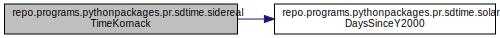
\includegraphics[width=350pt]{namespacerepo_1_1programs_1_1pythonpackages_1_1pr_1_1sdtime_a5247b0c3e822a26482ae1a8d008b2ec6_cgraph}
\end{center}
\end{figure}


\hypertarget{namespacerepo_1_1programs_1_1pythonpackages_1_1pr_1_1sdtime_ad97ec56a6ba609ebcc68f1734ec3d8d5}{\index{repo\-::programs\-::pythonpackages\-::pr\-::sdtime@{repo\-::programs\-::pythonpackages\-::pr\-::sdtime}!sidereal\-Time\-Me@{sidereal\-Time\-Me}}
\index{sidereal\-Time\-Me@{sidereal\-Time\-Me}!repo::programs::pythonpackages::pr::sdtime@{repo\-::programs\-::pythonpackages\-::pr\-::sdtime}}
\subsubsection[{sidereal\-Time\-Me}]{\setlength{\rightskip}{0pt plus 5cm}def repo.\-programs.\-pythonpackages.\-pr.\-sdtime.\-sidereal\-Time\-Me (
\begin{DoxyParamCaption}
\item[{}]{T = {\ttfamily None}}
\end{DoxyParamCaption}
)}}\label{namespacerepo_1_1programs_1_1pythonpackages_1_1pr_1_1sdtime_ad97ec56a6ba609ebcc68f1734ec3d8d5}


Definition at line 47 of file sdtime.\-py.

\hypertarget{namespacerepo_1_1programs_1_1pythonpackages_1_1pr_1_1sdtime_a9c31dc1e910e733dd210a93a75cc56b6}{\index{repo\-::programs\-::pythonpackages\-::pr\-::sdtime@{repo\-::programs\-::pythonpackages\-::pr\-::sdtime}!sidereal\-Time\-Meesus@{sidereal\-Time\-Meesus}}
\index{sidereal\-Time\-Meesus@{sidereal\-Time\-Meesus}!repo::programs::pythonpackages::pr::sdtime@{repo\-::programs\-::pythonpackages\-::pr\-::sdtime}}
\subsubsection[{sidereal\-Time\-Meesus}]{\setlength{\rightskip}{0pt plus 5cm}def repo.\-programs.\-pythonpackages.\-pr.\-sdtime.\-sidereal\-Time\-Meesus (
\begin{DoxyParamCaption}
\item[{}]{T = {\ttfamily None}}
\end{DoxyParamCaption}
)}}\label{namespacerepo_1_1programs_1_1pythonpackages_1_1pr_1_1sdtime_a9c31dc1e910e733dd210a93a75cc56b6}


Definition at line 42 of file sdtime.\-py.

\hypertarget{namespacerepo_1_1programs_1_1pythonpackages_1_1pr_1_1sdtime_ac3c7ee3324f1c4723a245f4ddf08cd41}{\index{repo\-::programs\-::pythonpackages\-::pr\-::sdtime@{repo\-::programs\-::pythonpackages\-::pr\-::sdtime}!solar\-Days\-Since\-Y2000@{solar\-Days\-Since\-Y2000}}
\index{solar\-Days\-Since\-Y2000@{solar\-Days\-Since\-Y2000}!repo::programs::pythonpackages::pr::sdtime@{repo\-::programs\-::pythonpackages\-::pr\-::sdtime}}
\subsubsection[{solar\-Days\-Since\-Y2000}]{\setlength{\rightskip}{0pt plus 5cm}def repo.\-programs.\-pythonpackages.\-pr.\-sdtime.\-solar\-Days\-Since\-Y2000 (
\begin{DoxyParamCaption}
\item[{}]{unix\-Time = {\ttfamily None}}
\end{DoxyParamCaption}
)}}\label{namespacerepo_1_1programs_1_1pythonpackages_1_1pr_1_1sdtime_ac3c7ee3324f1c4723a245f4ddf08cd41}


Definition at line 34 of file sdtime.\-py.



Here is the caller graph for this function\-:
\nopagebreak
\begin{figure}[H]
\begin{center}
\leavevmode
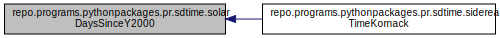
\includegraphics[width=350pt]{namespacerepo_1_1programs_1_1pythonpackages_1_1pr_1_1sdtime_ac3c7ee3324f1c4723a245f4ddf08cd41_icgraph}
\end{center}
\end{figure}




\subsection{Variable Documentation}
\hypertarget{namespacerepo_1_1programs_1_1pythonpackages_1_1pr_1_1sdtime_abe29426e8a972325a35a61402a87f188}{\index{repo\-::programs\-::pythonpackages\-::pr\-::sdtime@{repo\-::programs\-::pythonpackages\-::pr\-::sdtime}!F\-F@{F\-F}}
\index{F\-F@{F\-F}!repo::programs::pythonpackages::pr::sdtime@{repo\-::programs\-::pythonpackages\-::pr\-::sdtime}}
\subsubsection[{F\-F}]{\setlength{\rightskip}{0pt plus 5cm}float repo.\-programs.\-pythonpackages.\-pr.\-sdtime.\-F\-F = 0.\-277715}}\label{namespacerepo_1_1programs_1_1pythonpackages_1_1pr_1_1sdtime_abe29426e8a972325a35a61402a87f188}


Definition at line 7 of file sdtime.\-py.

\hypertarget{namespacerepo_1_1programs_1_1pythonpackages_1_1pr_1_1sdtime_ac9d3c2155d402d7c140fe3247e1f5722}{\index{repo\-::programs\-::pythonpackages\-::pr\-::sdtime@{repo\-::programs\-::pythonpackages\-::pr\-::sdtime}!secs\-Per\-Sid\-Day@{secs\-Per\-Sid\-Day}}
\index{secs\-Per\-Sid\-Day@{secs\-Per\-Sid\-Day}!repo::programs::pythonpackages::pr::sdtime@{repo\-::programs\-::pythonpackages\-::pr\-::sdtime}}
\subsubsection[{secs\-Per\-Sid\-Day}]{\setlength{\rightskip}{0pt plus 5cm}float repo.\-programs.\-pythonpackages.\-pr.\-sdtime.\-secs\-Per\-Sid\-Day = 86164.\-0905}}\label{namespacerepo_1_1programs_1_1pythonpackages_1_1pr_1_1sdtime_ac9d3c2155d402d7c140fe3247e1f5722}


Definition at line 6 of file sdtime.\-py.

\hypertarget{namespacerepo_1_1programs_1_1pythonpackages_1_1pr_1_1sdtime_ad0dcc84eadafdd803d57e73ef2c6e4a2}{\index{repo\-::programs\-::pythonpackages\-::pr\-::sdtime@{repo\-::programs\-::pythonpackages\-::pr\-::sdtime}!y2000secs@{y2000secs}}
\index{y2000secs@{y2000secs}!repo::programs::pythonpackages::pr::sdtime@{repo\-::programs\-::pythonpackages\-::pr\-::sdtime}}
\subsubsection[{y2000secs}]{\setlength{\rightskip}{0pt plus 5cm}int repo.\-programs.\-pythonpackages.\-pr.\-sdtime.\-y2000secs = 946684800}}\label{namespacerepo_1_1programs_1_1pythonpackages_1_1pr_1_1sdtime_ad0dcc84eadafdd803d57e73ef2c6e4a2}


Definition at line 5 of file sdtime.\-py.


\hypertarget{namespacerepo_1_1programs_1_1pythonpackages_1_1pr_1_1SPDataSet}{\section{repo.\-programs.\-pythonpackages.\-pr.\-S\-P\-Data\-Set Namespace Reference}
\label{namespacerepo_1_1programs_1_1pythonpackages_1_1pr_1_1SPDataSet}\index{repo.\-programs.\-pythonpackages.\-pr.\-S\-P\-Data\-Set@{repo.\-programs.\-pythonpackages.\-pr.\-S\-P\-Data\-Set}}
}
\subsection*{Classes}
\begin{DoxyCompactItemize}
\item 
class \hyperlink{classrepo_1_1programs_1_1pythonpackages_1_1pr_1_1SPDataSet_1_1SPDataSet}{S\-P\-Data\-Set}
\end{DoxyCompactItemize}
\subsection*{Functions}
\begin{DoxyCompactItemize}
\item 
def \hyperlink{namespacerepo_1_1programs_1_1pythonpackages_1_1pr_1_1SPDataSet_a296fa19993c2ac2fa6db975b8b0f6b88}{divide\-\_\-args\-\_\-memo}
\item 
def \hyperlink{namespacerepo_1_1programs_1_1pythonpackages_1_1pr_1_1SPDataSet_a9d0e07e3e1f4360be4f8c59927abe142}{divide\-\_\-args}
\begin{DoxyCompactList}\small\item\em Helpful for calling work\-\_\-func(following\-\_\-func($\ast$$\ast$remaining\-\_\-args), $\ast$$\ast$work\-\_\-args)) work\-\_\-args are the entries of cur\-\_\-kwargs that are in the argument list of work\-\_\-func. \end{DoxyCompactList}\item 
def \hyperlink{namespacerepo_1_1programs_1_1pythonpackages_1_1pr_1_1SPDataSet_a5a94fa78adaa1ce53cae1e69c7a10c1f}{gen\-Seq\-Filt\-Pol}
\begin{DoxyCompactList}\small\item\em Processing functions. \end{DoxyCompactList}\item 
def \hyperlink{namespacerepo_1_1programs_1_1pythonpackages_1_1pr_1_1SPDataSet_aee5e268a39b4f3d7d26b8cd8c2eb0dce}{seq\-Filt\-Func\-Axis\-Interleave}
\item 
def \hyperlink{namespacerepo_1_1programs_1_1pythonpackages_1_1pr_1_1SPDataSet_acf5db24745ff3b8a02816869e9b10482}{seq\-Filt\-Func\-Axis}
\item 
def \hyperlink{namespacerepo_1_1programs_1_1pythonpackages_1_1pr_1_1SPDataSet_aae98530dd28697279534ad7dd042acd8}{seq\-Filt\-Func2\-Axes}
\item 
def \hyperlink{namespacerepo_1_1programs_1_1pythonpackages_1_1pr_1_1SPDataSet_aa23a4db7857d6d485ae098e21e29cf59}{seq\-Filt\-Func\-Angle}
\item 
def \hyperlink{namespacerepo_1_1programs_1_1pythonpackages_1_1pr_1_1SPDataSet_abc13a280637f719ae917c9f2cf2d9d47}{seq\-Filt\-Func\-Slc}
\item 
def \hyperlink{namespacerepo_1_1programs_1_1pythonpackages_1_1pr_1_1SPDataSet_ae9bed330120419db29ade2d021ca34d7}{seq\-Filt\-Func\-Interleave}
\item 
def \hyperlink{namespacerepo_1_1programs_1_1pythonpackages_1_1pr_1_1SPDataSet_ac07feedd7af03661a0925bdec0d1f1fe}{seq\-Filt\-Func\-Time}
\item 
def \hyperlink{namespacerepo_1_1programs_1_1pythonpackages_1_1pr_1_1SPDataSet_af6b0d8ee29678751051a0b15362f9949}{check\-D\-S\-Unc}
\item 
def \hyperlink{namespacerepo_1_1programs_1_1pythonpackages_1_1pr_1_1SPDataSet_ab3e94a5db004f2a1cbe3b89005731d7c}{test\-D\-S}
\item 
def \hyperlink{namespacerepo_1_1programs_1_1pythonpackages_1_1pr_1_1SPDataSet_ae343b1ec862928d74ae9f6e140008b0d}{test\-D\-S2}
\end{DoxyCompactItemize}
\subsection*{Variables}
\begin{DoxyCompactItemize}
\item 
tuple \hyperlink{namespacerepo_1_1programs_1_1pythonpackages_1_1pr_1_1SPDataSet_ae71666498d0f08a9d2c39f65c8be15e1}{d} = dict(sig\-Window=Window(4,-\/5))
\item 
list \hyperlink{namespacerepo_1_1programs_1_1pythonpackages_1_1pr_1_1SPDataSet_aaa1cf30f24f4635798c2ac9ab8cb991f}{sid\-Amp\-L} = \mbox{[}$\,$\mbox{]}
\item 
tuple \hyperlink{namespacerepo_1_1programs_1_1pythonpackages_1_1pr_1_1SPDataSet_a6b49ba99ee674be07d78e57e0d6a4506}{rs\-Base} = Rotation\-Spec(starting\-Angle=0, delay=9, interval=10, num\-Rotations=20, rot\-Angles=\mbox{[}-\/180\mbox{]}, extra\-Rot\-Angle=-\/90)
\item 
list \hyperlink{namespacerepo_1_1programs_1_1pythonpackages_1_1pr_1_1SPDataSet_a794711a619d88291abbe1c9c29396b5b}{rs\-L} = \mbox{[}rs\-Base.\-\_\-replace(starting\-Angle=th) for th in hstack(\mbox{[}zeros(15), -\/ones(0)$\ast$90, ones(0)$\ast$45\mbox{]})\mbox{]}
\item 
tuple \hyperlink{namespacerepo_1_1programs_1_1pythonpackages_1_1pr_1_1SPDataSet_a9dcba74d2fb20a6a41c191302ec5136b}{ds} = \hyperlink{classrepo_1_1programs_1_1pythonpackages_1_1pr_1_1SPDataSet_1_1SPDataSet}{S\-P\-Data\-Set}('test', preload\-Dict=\{'fast\-D'\-: \mbox{[}sd, sig, 'sig'\mbox{]}\}, r\-Spec=rs )
\item 
tuple \hyperlink{namespacerepo_1_1programs_1_1pythonpackages_1_1pr_1_1SPDataSet_a7ef84c87edaf55c60c75aa4a6b63fabf}{s\-Amp} = ds.\-sid\-Amp(sig\-Window=Window(4,-\/5))
\item 
list \hyperlink{namespacerepo_1_1programs_1_1pythonpackages_1_1pr_1_1SPDataSet_ab977d64bf78ed1ce32101398d66e2673}{timestamp\-L}
\item 
list \hyperlink{namespacerepo_1_1programs_1_1pythonpackages_1_1pr_1_1SPDataSet_a2e421078d46e1d8f3b0c2d7c8211e1a2}{ts} = \mbox{[} s\-Amp.\-t for \hyperlink{namespacerepo_1_1programs_1_1pythonpackages_1_1pr_1_1SPDataSet_a7ef84c87edaf55c60c75aa4a6b63fabf}{s\-Amp} in \hyperlink{namespacerepo_1_1programs_1_1pythonpackages_1_1pr_1_1SPDataSet_aaa1cf30f24f4635798c2ac9ab8cb991f}{sid\-Amp\-L}\mbox{]}
\item 
tuple \hyperlink{namespacerepo_1_1programs_1_1pythonpackages_1_1pr_1_1SPDataSet_af4556d66bac96baab9aed887e66ce083}{ys} = array(ys)
\item 
tuple \hyperlink{namespacerepo_1_1programs_1_1pythonpackages_1_1pr_1_1SPDataSet_a3c7145cc42e7ec16a596f5996a8e70e2}{errs} = array(\mbox{[}sqrt(cov.\-diagonal()) for cov in covs\mbox{]})
\item 
string \hyperlink{namespacerepo_1_1programs_1_1pythonpackages_1_1pr_1_1SPDataSet_aa809f797a727977783e89201eb7515ba}{st} = ''
\end{DoxyCompactItemize}


\subsection{Function Documentation}
\hypertarget{namespacerepo_1_1programs_1_1pythonpackages_1_1pr_1_1SPDataSet_af6b0d8ee29678751051a0b15362f9949}{\index{repo\-::programs\-::pythonpackages\-::pr\-::\-S\-P\-Data\-Set@{repo\-::programs\-::pythonpackages\-::pr\-::\-S\-P\-Data\-Set}!check\-D\-S\-Unc@{check\-D\-S\-Unc}}
\index{check\-D\-S\-Unc@{check\-D\-S\-Unc}!repo::programs::pythonpackages::pr::SPDataSet@{repo\-::programs\-::pythonpackages\-::pr\-::\-S\-P\-Data\-Set}}
\subsubsection[{check\-D\-S\-Unc}]{\setlength{\rightskip}{0pt plus 5cm}def repo.\-programs.\-pythonpackages.\-pr.\-S\-P\-Data\-Set.\-check\-D\-S\-Unc (
\begin{DoxyParamCaption}
\item[{}]{ds, }
\item[{}]{Ndiv = {\ttfamily 10}, }
\item[{}]{kwargs}
\end{DoxyParamCaption}
)}}\label{namespacerepo_1_1programs_1_1pythonpackages_1_1pr_1_1SPDataSet_af6b0d8ee29678751051a0b15362f9949}


Definition at line 688 of file S\-P\-Data\-Set.\-py.



Here is the call graph for this function\-:
\nopagebreak
\begin{figure}[H]
\begin{center}
\leavevmode
\includegraphics[width=350pt]{namespacerepo_1_1programs_1_1pythonpackages_1_1pr_1_1SPDataSet_af6b0d8ee29678751051a0b15362f9949_cgraph}
\end{center}
\end{figure}


\hypertarget{namespacerepo_1_1programs_1_1pythonpackages_1_1pr_1_1SPDataSet_a9d0e07e3e1f4360be4f8c59927abe142}{\index{repo\-::programs\-::pythonpackages\-::pr\-::\-S\-P\-Data\-Set@{repo\-::programs\-::pythonpackages\-::pr\-::\-S\-P\-Data\-Set}!divide\-\_\-args@{divide\-\_\-args}}
\index{divide\-\_\-args@{divide\-\_\-args}!repo::programs::pythonpackages::pr::SPDataSet@{repo\-::programs\-::pythonpackages\-::pr\-::\-S\-P\-Data\-Set}}
\subsubsection[{divide\-\_\-args}]{\setlength{\rightskip}{0pt plus 5cm}def repo.\-programs.\-pythonpackages.\-pr.\-S\-P\-Data\-Set.\-divide\-\_\-args (
\begin{DoxyParamCaption}
\item[{}]{cur\-\_\-kwargs, }
\item[{}]{work\-\_\-func}
\end{DoxyParamCaption}
)}}\label{namespacerepo_1_1programs_1_1pythonpackages_1_1pr_1_1SPDataSet_a9d0e07e3e1f4360be4f8c59927abe142}


Helpful for calling work\-\_\-func(following\-\_\-func($\ast$$\ast$remaining\-\_\-args), $\ast$$\ast$work\-\_\-args)) work\-\_\-args are the entries of cur\-\_\-kwargs that are in the argument list of work\-\_\-func. 

Remaining\-\_\-args are those left over Currently just returns the divided argument list 

Definition at line 34 of file S\-P\-Data\-Set.\-py.



Here is the caller graph for this function\-:
\nopagebreak
\begin{figure}[H]
\begin{center}
\leavevmode
\includegraphics[width=350pt]{namespacerepo_1_1programs_1_1pythonpackages_1_1pr_1_1SPDataSet_a9d0e07e3e1f4360be4f8c59927abe142_icgraph}
\end{center}
\end{figure}


\hypertarget{namespacerepo_1_1programs_1_1pythonpackages_1_1pr_1_1SPDataSet_a296fa19993c2ac2fa6db975b8b0f6b88}{\index{repo\-::programs\-::pythonpackages\-::pr\-::\-S\-P\-Data\-Set@{repo\-::programs\-::pythonpackages\-::pr\-::\-S\-P\-Data\-Set}!divide\-\_\-args\-\_\-memo@{divide\-\_\-args\-\_\-memo}}
\index{divide\-\_\-args\-\_\-memo@{divide\-\_\-args\-\_\-memo}!repo::programs::pythonpackages::pr::SPDataSet@{repo\-::programs\-::pythonpackages\-::pr\-::\-S\-P\-Data\-Set}}
\subsubsection[{divide\-\_\-args\-\_\-memo}]{\setlength{\rightskip}{0pt plus 5cm}def repo.\-programs.\-pythonpackages.\-pr.\-S\-P\-Data\-Set.\-divide\-\_\-args\-\_\-memo (
\begin{DoxyParamCaption}
\item[{}]{kwargs, }
\item[{}]{func\-\_\-to\-\_\-follow}
\end{DoxyParamCaption}
)}}\label{namespacerepo_1_1programs_1_1pythonpackages_1_1pr_1_1SPDataSet_a296fa19993c2ac2fa6db975b8b0f6b88}


Definition at line 24 of file S\-P\-Data\-Set.\-py.

\hypertarget{namespacerepo_1_1programs_1_1pythonpackages_1_1pr_1_1SPDataSet_a5a94fa78adaa1ce53cae1e69c7a10c1f}{\index{repo\-::programs\-::pythonpackages\-::pr\-::\-S\-P\-Data\-Set@{repo\-::programs\-::pythonpackages\-::pr\-::\-S\-P\-Data\-Set}!gen\-Seq\-Filt\-Pol@{gen\-Seq\-Filt\-Pol}}
\index{gen\-Seq\-Filt\-Pol@{gen\-Seq\-Filt\-Pol}!repo::programs::pythonpackages::pr::SPDataSet@{repo\-::programs\-::pythonpackages\-::pr\-::\-S\-P\-Data\-Set}}
\subsubsection[{gen\-Seq\-Filt\-Pol}]{\setlength{\rightskip}{0pt plus 5cm}def repo.\-programs.\-pythonpackages.\-pr.\-S\-P\-Data\-Set.\-gen\-Seq\-Filt\-Pol (
\begin{DoxyParamCaption}
\item[{}]{sgn}
\end{DoxyParamCaption}
)}}\label{namespacerepo_1_1programs_1_1pythonpackages_1_1pr_1_1SPDataSet_a5a94fa78adaa1ce53cae1e69c7a10c1f}


Processing functions. 



Definition at line 623 of file S\-P\-Data\-Set.\-py.

\hypertarget{namespacerepo_1_1programs_1_1pythonpackages_1_1pr_1_1SPDataSet_aae98530dd28697279534ad7dd042acd8}{\index{repo\-::programs\-::pythonpackages\-::pr\-::\-S\-P\-Data\-Set@{repo\-::programs\-::pythonpackages\-::pr\-::\-S\-P\-Data\-Set}!seq\-Filt\-Func2\-Axes@{seq\-Filt\-Func2\-Axes}}
\index{seq\-Filt\-Func2\-Axes@{seq\-Filt\-Func2\-Axes}!repo::programs::pythonpackages::pr::SPDataSet@{repo\-::programs\-::pythonpackages\-::pr\-::\-S\-P\-Data\-Set}}
\subsubsection[{seq\-Filt\-Func2\-Axes}]{\setlength{\rightskip}{0pt plus 5cm}def repo.\-programs.\-pythonpackages.\-pr.\-S\-P\-Data\-Set.\-seq\-Filt\-Func2\-Axes (
\begin{DoxyParamCaption}
\item[{}]{axis\-Angle}
\end{DoxyParamCaption}
)}}\label{namespacerepo_1_1programs_1_1pythonpackages_1_1pr_1_1SPDataSet_aae98530dd28697279534ad7dd042acd8}


Definition at line 646 of file S\-P\-Data\-Set.\-py.

\hypertarget{namespacerepo_1_1programs_1_1pythonpackages_1_1pr_1_1SPDataSet_aa23a4db7857d6d485ae098e21e29cf59}{\index{repo\-::programs\-::pythonpackages\-::pr\-::\-S\-P\-Data\-Set@{repo\-::programs\-::pythonpackages\-::pr\-::\-S\-P\-Data\-Set}!seq\-Filt\-Func\-Angle@{seq\-Filt\-Func\-Angle}}
\index{seq\-Filt\-Func\-Angle@{seq\-Filt\-Func\-Angle}!repo::programs::pythonpackages::pr::SPDataSet@{repo\-::programs\-::pythonpackages\-::pr\-::\-S\-P\-Data\-Set}}
\subsubsection[{seq\-Filt\-Func\-Angle}]{\setlength{\rightskip}{0pt plus 5cm}def repo.\-programs.\-pythonpackages.\-pr.\-S\-P\-Data\-Set.\-seq\-Filt\-Func\-Angle (
\begin{DoxyParamCaption}
\item[{}]{angle}
\end{DoxyParamCaption}
)}}\label{namespacerepo_1_1programs_1_1pythonpackages_1_1pr_1_1SPDataSet_aa23a4db7857d6d485ae098e21e29cf59}


Definition at line 655 of file S\-P\-Data\-Set.\-py.

\hypertarget{namespacerepo_1_1programs_1_1pythonpackages_1_1pr_1_1SPDataSet_acf5db24745ff3b8a02816869e9b10482}{\index{repo\-::programs\-::pythonpackages\-::pr\-::\-S\-P\-Data\-Set@{repo\-::programs\-::pythonpackages\-::pr\-::\-S\-P\-Data\-Set}!seq\-Filt\-Func\-Axis@{seq\-Filt\-Func\-Axis}}
\index{seq\-Filt\-Func\-Axis@{seq\-Filt\-Func\-Axis}!repo::programs::pythonpackages::pr::SPDataSet@{repo\-::programs\-::pythonpackages\-::pr\-::\-S\-P\-Data\-Set}}
\subsubsection[{seq\-Filt\-Func\-Axis}]{\setlength{\rightskip}{0pt plus 5cm}def repo.\-programs.\-pythonpackages.\-pr.\-S\-P\-Data\-Set.\-seq\-Filt\-Func\-Axis (
\begin{DoxyParamCaption}
\item[{}]{axis\-Angle}
\end{DoxyParamCaption}
)}}\label{namespacerepo_1_1programs_1_1pythonpackages_1_1pr_1_1SPDataSet_acf5db24745ff3b8a02816869e9b10482}


Definition at line 638 of file S\-P\-Data\-Set.\-py.



Here is the caller graph for this function\-:
\nopagebreak
\begin{figure}[H]
\begin{center}
\leavevmode
\includegraphics[width=350pt]{namespacerepo_1_1programs_1_1pythonpackages_1_1pr_1_1SPDataSet_acf5db24745ff3b8a02816869e9b10482_icgraph}
\end{center}
\end{figure}


\hypertarget{namespacerepo_1_1programs_1_1pythonpackages_1_1pr_1_1SPDataSet_aee5e268a39b4f3d7d26b8cd8c2eb0dce}{\index{repo\-::programs\-::pythonpackages\-::pr\-::\-S\-P\-Data\-Set@{repo\-::programs\-::pythonpackages\-::pr\-::\-S\-P\-Data\-Set}!seq\-Filt\-Func\-Axis\-Interleave@{seq\-Filt\-Func\-Axis\-Interleave}}
\index{seq\-Filt\-Func\-Axis\-Interleave@{seq\-Filt\-Func\-Axis\-Interleave}!repo::programs::pythonpackages::pr::SPDataSet@{repo\-::programs\-::pythonpackages\-::pr\-::\-S\-P\-Data\-Set}}
\subsubsection[{seq\-Filt\-Func\-Axis\-Interleave}]{\setlength{\rightskip}{0pt plus 5cm}def repo.\-programs.\-pythonpackages.\-pr.\-S\-P\-Data\-Set.\-seq\-Filt\-Func\-Axis\-Interleave (
\begin{DoxyParamCaption}
\item[{}]{axis\-Angle, }
\item[{}]{Ndiv}
\end{DoxyParamCaption}
)}}\label{namespacerepo_1_1programs_1_1pythonpackages_1_1pr_1_1SPDataSet_aee5e268a39b4f3d7d26b8cd8c2eb0dce}


Definition at line 632 of file S\-P\-Data\-Set.\-py.



Here is the call graph for this function\-:
\nopagebreak
\begin{figure}[H]
\begin{center}
\leavevmode
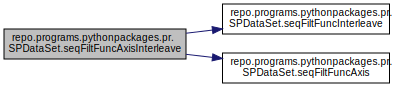
\includegraphics[width=350pt]{namespacerepo_1_1programs_1_1pythonpackages_1_1pr_1_1SPDataSet_aee5e268a39b4f3d7d26b8cd8c2eb0dce_cgraph}
\end{center}
\end{figure}


\hypertarget{namespacerepo_1_1programs_1_1pythonpackages_1_1pr_1_1SPDataSet_ae9bed330120419db29ade2d021ca34d7}{\index{repo\-::programs\-::pythonpackages\-::pr\-::\-S\-P\-Data\-Set@{repo\-::programs\-::pythonpackages\-::pr\-::\-S\-P\-Data\-Set}!seq\-Filt\-Func\-Interleave@{seq\-Filt\-Func\-Interleave}}
\index{seq\-Filt\-Func\-Interleave@{seq\-Filt\-Func\-Interleave}!repo::programs::pythonpackages::pr::SPDataSet@{repo\-::programs\-::pythonpackages\-::pr\-::\-S\-P\-Data\-Set}}
\subsubsection[{seq\-Filt\-Func\-Interleave}]{\setlength{\rightskip}{0pt plus 5cm}def repo.\-programs.\-pythonpackages.\-pr.\-S\-P\-Data\-Set.\-seq\-Filt\-Func\-Interleave (
\begin{DoxyParamCaption}
\item[{}]{Ndiv}
\end{DoxyParamCaption}
)}}\label{namespacerepo_1_1programs_1_1pythonpackages_1_1pr_1_1SPDataSet_ae9bed330120419db29ade2d021ca34d7}


Definition at line 666 of file S\-P\-Data\-Set.\-py.



Here is the caller graph for this function\-:
\nopagebreak
\begin{figure}[H]
\begin{center}
\leavevmode
\includegraphics[width=350pt]{namespacerepo_1_1programs_1_1pythonpackages_1_1pr_1_1SPDataSet_ae9bed330120419db29ade2d021ca34d7_icgraph}
\end{center}
\end{figure}


\hypertarget{namespacerepo_1_1programs_1_1pythonpackages_1_1pr_1_1SPDataSet_abc13a280637f719ae917c9f2cf2d9d47}{\index{repo\-::programs\-::pythonpackages\-::pr\-::\-S\-P\-Data\-Set@{repo\-::programs\-::pythonpackages\-::pr\-::\-S\-P\-Data\-Set}!seq\-Filt\-Func\-Slc@{seq\-Filt\-Func\-Slc}}
\index{seq\-Filt\-Func\-Slc@{seq\-Filt\-Func\-Slc}!repo::programs::pythonpackages::pr::SPDataSet@{repo\-::programs\-::pythonpackages\-::pr\-::\-S\-P\-Data\-Set}}
\subsubsection[{seq\-Filt\-Func\-Slc}]{\setlength{\rightskip}{0pt plus 5cm}def repo.\-programs.\-pythonpackages.\-pr.\-S\-P\-Data\-Set.\-seq\-Filt\-Func\-Slc (
\begin{DoxyParamCaption}
\item[{}]{slc}
\end{DoxyParamCaption}
)}}\label{namespacerepo_1_1programs_1_1pythonpackages_1_1pr_1_1SPDataSet_abc13a280637f719ae917c9f2cf2d9d47}


Definition at line 661 of file S\-P\-Data\-Set.\-py.

\hypertarget{namespacerepo_1_1programs_1_1pythonpackages_1_1pr_1_1SPDataSet_ac07feedd7af03661a0925bdec0d1f1fe}{\index{repo\-::programs\-::pythonpackages\-::pr\-::\-S\-P\-Data\-Set@{repo\-::programs\-::pythonpackages\-::pr\-::\-S\-P\-Data\-Set}!seq\-Filt\-Func\-Time@{seq\-Filt\-Func\-Time}}
\index{seq\-Filt\-Func\-Time@{seq\-Filt\-Func\-Time}!repo::programs::pythonpackages::pr::SPDataSet@{repo\-::programs\-::pythonpackages\-::pr\-::\-S\-P\-Data\-Set}}
\subsubsection[{seq\-Filt\-Func\-Time}]{\setlength{\rightskip}{0pt plus 5cm}def repo.\-programs.\-pythonpackages.\-pr.\-S\-P\-Data\-Set.\-seq\-Filt\-Func\-Time (
\begin{DoxyParamCaption}
\item[{}]{Tdiv = {\ttfamily 1}}
\end{DoxyParamCaption}
)}}\label{namespacerepo_1_1programs_1_1pythonpackages_1_1pr_1_1SPDataSet_ac07feedd7af03661a0925bdec0d1f1fe}


Definition at line 678 of file S\-P\-Data\-Set.\-py.



Here is the call graph for this function\-:
\nopagebreak
\begin{figure}[H]
\begin{center}
\leavevmode
\includegraphics[width=350pt]{namespacerepo_1_1programs_1_1pythonpackages_1_1pr_1_1SPDataSet_ac07feedd7af03661a0925bdec0d1f1fe_cgraph}
\end{center}
\end{figure}


\hypertarget{namespacerepo_1_1programs_1_1pythonpackages_1_1pr_1_1SPDataSet_ab3e94a5db004f2a1cbe3b89005731d7c}{\index{repo\-::programs\-::pythonpackages\-::pr\-::\-S\-P\-Data\-Set@{repo\-::programs\-::pythonpackages\-::pr\-::\-S\-P\-Data\-Set}!test\-D\-S@{test\-D\-S}}
\index{test\-D\-S@{test\-D\-S}!repo::programs::pythonpackages::pr::SPDataSet@{repo\-::programs\-::pythonpackages\-::pr\-::\-S\-P\-Data\-Set}}
\subsubsection[{test\-D\-S}]{\setlength{\rightskip}{0pt plus 5cm}def repo.\-programs.\-pythonpackages.\-pr.\-S\-P\-Data\-Set.\-test\-D\-S (
\begin{DoxyParamCaption}
\item[{}]{r\-Spec = {\ttfamily None}, }
\item[{}]{rot\-Fact = {\ttfamily 1}, }
\item[{}]{kwargs}
\end{DoxyParamCaption}
)}}\label{namespacerepo_1_1programs_1_1pythonpackages_1_1pr_1_1SPDataSet_ab3e94a5db004f2a1cbe3b89005731d7c}


Definition at line 709 of file S\-P\-Data\-Set.\-py.



Here is the call graph for this function\-:
\nopagebreak
\begin{figure}[H]
\begin{center}
\leavevmode
\includegraphics[width=350pt]{namespacerepo_1_1programs_1_1pythonpackages_1_1pr_1_1SPDataSet_ab3e94a5db004f2a1cbe3b89005731d7c_cgraph}
\end{center}
\end{figure}


\hypertarget{namespacerepo_1_1programs_1_1pythonpackages_1_1pr_1_1SPDataSet_ae343b1ec862928d74ae9f6e140008b0d}{\index{repo\-::programs\-::pythonpackages\-::pr\-::\-S\-P\-Data\-Set@{repo\-::programs\-::pythonpackages\-::pr\-::\-S\-P\-Data\-Set}!test\-D\-S2@{test\-D\-S2}}
\index{test\-D\-S2@{test\-D\-S2}!repo::programs::pythonpackages::pr::SPDataSet@{repo\-::programs\-::pythonpackages\-::pr\-::\-S\-P\-Data\-Set}}
\subsubsection[{test\-D\-S2}]{\setlength{\rightskip}{0pt plus 5cm}def repo.\-programs.\-pythonpackages.\-pr.\-S\-P\-Data\-Set.\-test\-D\-S2 (
\begin{DoxyParamCaption}
\item[{}]{r\-Spec = {\ttfamily None}, }
\item[{}]{rot\-Dir = {\ttfamily 1}, }
\item[{}]{kwargs}
\end{DoxyParamCaption}
)}}\label{namespacerepo_1_1programs_1_1pythonpackages_1_1pr_1_1SPDataSet_ae343b1ec862928d74ae9f6e140008b0d}


Definition at line 722 of file S\-P\-Data\-Set.\-py.



Here is the call graph for this function\-:
\nopagebreak
\begin{figure}[H]
\begin{center}
\leavevmode
\includegraphics[width=350pt]{namespacerepo_1_1programs_1_1pythonpackages_1_1pr_1_1SPDataSet_ae343b1ec862928d74ae9f6e140008b0d_cgraph}
\end{center}
\end{figure}




\subsection{Variable Documentation}
\hypertarget{namespacerepo_1_1programs_1_1pythonpackages_1_1pr_1_1SPDataSet_ae71666498d0f08a9d2c39f65c8be15e1}{\index{repo\-::programs\-::pythonpackages\-::pr\-::\-S\-P\-Data\-Set@{repo\-::programs\-::pythonpackages\-::pr\-::\-S\-P\-Data\-Set}!d@{d}}
\index{d@{d}!repo::programs::pythonpackages::pr::SPDataSet@{repo\-::programs\-::pythonpackages\-::pr\-::\-S\-P\-Data\-Set}}
\subsubsection[{d}]{\setlength{\rightskip}{0pt plus 5cm}tuple repo.\-programs.\-pythonpackages.\-pr.\-S\-P\-Data\-Set.\-d = dict(sig\-Window=Window(4,-\/5))}}\label{namespacerepo_1_1programs_1_1pythonpackages_1_1pr_1_1SPDataSet_ae71666498d0f08a9d2c39f65c8be15e1}


Definition at line 736 of file S\-P\-Data\-Set.\-py.

\hypertarget{namespacerepo_1_1programs_1_1pythonpackages_1_1pr_1_1SPDataSet_a9dcba74d2fb20a6a41c191302ec5136b}{\index{repo\-::programs\-::pythonpackages\-::pr\-::\-S\-P\-Data\-Set@{repo\-::programs\-::pythonpackages\-::pr\-::\-S\-P\-Data\-Set}!ds@{ds}}
\index{ds@{ds}!repo::programs::pythonpackages::pr::SPDataSet@{repo\-::programs\-::pythonpackages\-::pr\-::\-S\-P\-Data\-Set}}
\subsubsection[{ds}]{\setlength{\rightskip}{0pt plus 5cm}tuple repo.\-programs.\-pythonpackages.\-pr.\-S\-P\-Data\-Set.\-ds = {\bf S\-P\-Data\-Set}('test', preload\-Dict=\{'fast\-D'\-: \mbox{[}sd, sig, 'sig'\mbox{]}\}, r\-Spec=rs )}}\label{namespacerepo_1_1programs_1_1pythonpackages_1_1pr_1_1SPDataSet_a9dcba74d2fb20a6a41c191302ec5136b}


Definition at line 746 of file S\-P\-Data\-Set.\-py.

\hypertarget{namespacerepo_1_1programs_1_1pythonpackages_1_1pr_1_1SPDataSet_a3c7145cc42e7ec16a596f5996a8e70e2}{\index{repo\-::programs\-::pythonpackages\-::pr\-::\-S\-P\-Data\-Set@{repo\-::programs\-::pythonpackages\-::pr\-::\-S\-P\-Data\-Set}!errs@{errs}}
\index{errs@{errs}!repo::programs::pythonpackages::pr::SPDataSet@{repo\-::programs\-::pythonpackages\-::pr\-::\-S\-P\-Data\-Set}}
\subsubsection[{errs}]{\setlength{\rightskip}{0pt plus 5cm}tuple repo.\-programs.\-pythonpackages.\-pr.\-S\-P\-Data\-Set.\-errs = array(\mbox{[}sqrt(cov.\-diagonal()) for cov in covs\mbox{]})}}\label{namespacerepo_1_1programs_1_1pythonpackages_1_1pr_1_1SPDataSet_a3c7145cc42e7ec16a596f5996a8e70e2}


Definition at line 801 of file S\-P\-Data\-Set.\-py.

\hypertarget{namespacerepo_1_1programs_1_1pythonpackages_1_1pr_1_1SPDataSet_a6b49ba99ee674be07d78e57e0d6a4506}{\index{repo\-::programs\-::pythonpackages\-::pr\-::\-S\-P\-Data\-Set@{repo\-::programs\-::pythonpackages\-::pr\-::\-S\-P\-Data\-Set}!rs\-Base@{rs\-Base}}
\index{rs\-Base@{rs\-Base}!repo::programs::pythonpackages::pr::SPDataSet@{repo\-::programs\-::pythonpackages\-::pr\-::\-S\-P\-Data\-Set}}
\subsubsection[{rs\-Base}]{\setlength{\rightskip}{0pt plus 5cm}tuple repo.\-programs.\-pythonpackages.\-pr.\-S\-P\-Data\-Set.\-rs\-Base = Rotation\-Spec(starting\-Angle=0, delay=9, interval=10, num\-Rotations=20, rot\-Angles=\mbox{[}-\/180\mbox{]}, extra\-Rot\-Angle=-\/90)}}\label{namespacerepo_1_1programs_1_1pythonpackages_1_1pr_1_1SPDataSet_a6b49ba99ee674be07d78e57e0d6a4506}


Definition at line 740 of file S\-P\-Data\-Set.\-py.

\hypertarget{namespacerepo_1_1programs_1_1pythonpackages_1_1pr_1_1SPDataSet_a794711a619d88291abbe1c9c29396b5b}{\index{repo\-::programs\-::pythonpackages\-::pr\-::\-S\-P\-Data\-Set@{repo\-::programs\-::pythonpackages\-::pr\-::\-S\-P\-Data\-Set}!rs\-L@{rs\-L}}
\index{rs\-L@{rs\-L}!repo::programs::pythonpackages::pr::SPDataSet@{repo\-::programs\-::pythonpackages\-::pr\-::\-S\-P\-Data\-Set}}
\subsubsection[{rs\-L}]{\setlength{\rightskip}{0pt plus 5cm}list repo.\-programs.\-pythonpackages.\-pr.\-S\-P\-Data\-Set.\-rs\-L = \mbox{[}rs\-Base.\-\_\-replace(starting\-Angle=th) for th in hstack(\mbox{[}zeros(15), -\/ones(0)$\ast$90, ones(0)$\ast$45\mbox{]})\mbox{]}}}\label{namespacerepo_1_1programs_1_1pythonpackages_1_1pr_1_1SPDataSet_a794711a619d88291abbe1c9c29396b5b}


Definition at line 741 of file S\-P\-Data\-Set.\-py.

\hypertarget{namespacerepo_1_1programs_1_1pythonpackages_1_1pr_1_1SPDataSet_a7ef84c87edaf55c60c75aa4a6b63fabf}{\index{repo\-::programs\-::pythonpackages\-::pr\-::\-S\-P\-Data\-Set@{repo\-::programs\-::pythonpackages\-::pr\-::\-S\-P\-Data\-Set}!s\-Amp@{s\-Amp}}
\index{s\-Amp@{s\-Amp}!repo::programs::pythonpackages::pr::SPDataSet@{repo\-::programs\-::pythonpackages\-::pr\-::\-S\-P\-Data\-Set}}
\subsubsection[{s\-Amp}]{\setlength{\rightskip}{0pt plus 5cm}tuple repo.\-programs.\-pythonpackages.\-pr.\-S\-P\-Data\-Set.\-s\-Amp = ds.\-sid\-Amp(sig\-Window=Window(4,-\/5))}}\label{namespacerepo_1_1programs_1_1pythonpackages_1_1pr_1_1SPDataSet_a7ef84c87edaf55c60c75aa4a6b63fabf}


Definition at line 747 of file S\-P\-Data\-Set.\-py.

\hypertarget{namespacerepo_1_1programs_1_1pythonpackages_1_1pr_1_1SPDataSet_aaa1cf30f24f4635798c2ac9ab8cb991f}{\index{repo\-::programs\-::pythonpackages\-::pr\-::\-S\-P\-Data\-Set@{repo\-::programs\-::pythonpackages\-::pr\-::\-S\-P\-Data\-Set}!sid\-Amp\-L@{sid\-Amp\-L}}
\index{sid\-Amp\-L@{sid\-Amp\-L}!repo::programs::pythonpackages::pr::SPDataSet@{repo\-::programs\-::pythonpackages\-::pr\-::\-S\-P\-Data\-Set}}
\subsubsection[{sid\-Amp\-L}]{\setlength{\rightskip}{0pt plus 5cm}list repo.\-programs.\-pythonpackages.\-pr.\-S\-P\-Data\-Set.\-sid\-Amp\-L = \mbox{[}$\,$\mbox{]}}}\label{namespacerepo_1_1programs_1_1pythonpackages_1_1pr_1_1SPDataSet_aaa1cf30f24f4635798c2ac9ab8cb991f}


Definition at line 738 of file S\-P\-Data\-Set.\-py.

\hypertarget{namespacerepo_1_1programs_1_1pythonpackages_1_1pr_1_1SPDataSet_aa809f797a727977783e89201eb7515ba}{\index{repo\-::programs\-::pythonpackages\-::pr\-::\-S\-P\-Data\-Set@{repo\-::programs\-::pythonpackages\-::pr\-::\-S\-P\-Data\-Set}!st@{st}}
\index{st@{st}!repo::programs::pythonpackages::pr::SPDataSet@{repo\-::programs\-::pythonpackages\-::pr\-::\-S\-P\-Data\-Set}}
\subsubsection[{st}]{\setlength{\rightskip}{0pt plus 5cm}tuple repo.\-programs.\-pythonpackages.\-pr.\-S\-P\-Data\-Set.\-st = ''}}\label{namespacerepo_1_1programs_1_1pythonpackages_1_1pr_1_1SPDataSet_aa809f797a727977783e89201eb7515ba}


Definition at line 843 of file S\-P\-Data\-Set.\-py.

\hypertarget{namespacerepo_1_1programs_1_1pythonpackages_1_1pr_1_1SPDataSet_ab977d64bf78ed1ce32101398d66e2673}{\index{repo\-::programs\-::pythonpackages\-::pr\-::\-S\-P\-Data\-Set@{repo\-::programs\-::pythonpackages\-::pr\-::\-S\-P\-Data\-Set}!timestamp\-L@{timestamp\-L}}
\index{timestamp\-L@{timestamp\-L}!repo::programs::pythonpackages::pr::SPDataSet@{repo\-::programs\-::pythonpackages\-::pr\-::\-S\-P\-Data\-Set}}
\subsubsection[{timestamp\-L}]{\setlength{\rightskip}{0pt plus 5cm}list repo.\-programs.\-pythonpackages.\-pr.\-S\-P\-Data\-Set.\-timestamp\-L}}\label{namespacerepo_1_1programs_1_1pythonpackages_1_1pr_1_1SPDataSet_ab977d64bf78ed1ce32101398d66e2673}
{\bfseries Initial value\-:}
\begin{DoxyCode}
1 = [
2                     \textcolor{comment}{#'5209.26',}
3                     \textcolor{comment}{#'5240.33',}
4                     \textcolor{stringliteral}{'5249.72'},
5                     \textcolor{stringliteral}{'5273.74'},
6                     \textcolor{stringliteral}{'5282.23'},
7                     \textcolor{stringliteral}{'5292.71'},
8                     \textcolor{stringliteral}{'5294.31'},
9                     \textcolor{comment}{#'5296.33',}
10                     \textcolor{stringliteral}{'5310.41'},
11                     \textcolor{stringliteral}{'5318.41'},
12                     \textcolor{stringliteral}{'5348.82'},
13                     \textcolor{stringliteral}{'5369.87'},
14                     \textcolor{stringliteral}{'5386.02'},
15                     \textcolor{stringliteral}{'5390.74'},
16                 ]
\end{DoxyCode}


Definition at line 767 of file S\-P\-Data\-Set.\-py.

\hypertarget{namespacerepo_1_1programs_1_1pythonpackages_1_1pr_1_1SPDataSet_a2e421078d46e1d8f3b0c2d7c8211e1a2}{\index{repo\-::programs\-::pythonpackages\-::pr\-::\-S\-P\-Data\-Set@{repo\-::programs\-::pythonpackages\-::pr\-::\-S\-P\-Data\-Set}!ts@{ts}}
\index{ts@{ts}!repo::programs::pythonpackages::pr::SPDataSet@{repo\-::programs\-::pythonpackages\-::pr\-::\-S\-P\-Data\-Set}}
\subsubsection[{ts}]{\setlength{\rightskip}{0pt plus 5cm}tuple repo.\-programs.\-pythonpackages.\-pr.\-S\-P\-Data\-Set.\-ts = \mbox{[} s\-Amp.\-t for {\bf s\-Amp} in {\bf sid\-Amp\-L}\mbox{]}}}\label{namespacerepo_1_1programs_1_1pythonpackages_1_1pr_1_1SPDataSet_a2e421078d46e1d8f3b0c2d7c8211e1a2}


Definition at line 796 of file S\-P\-Data\-Set.\-py.

\hypertarget{namespacerepo_1_1programs_1_1pythonpackages_1_1pr_1_1SPDataSet_af4556d66bac96baab9aed887e66ce083}{\index{repo\-::programs\-::pythonpackages\-::pr\-::\-S\-P\-Data\-Set@{repo\-::programs\-::pythonpackages\-::pr\-::\-S\-P\-Data\-Set}!ys@{ys}}
\index{ys@{ys}!repo::programs::pythonpackages::pr::SPDataSet@{repo\-::programs\-::pythonpackages\-::pr\-::\-S\-P\-Data\-Set}}
\subsubsection[{ys}]{\setlength{\rightskip}{0pt plus 5cm}tuple repo.\-programs.\-pythonpackages.\-pr.\-S\-P\-Data\-Set.\-ys = array(ys)}}\label{namespacerepo_1_1programs_1_1pythonpackages_1_1pr_1_1SPDataSet_af4556d66bac96baab9aed887e66ce083}


Definition at line 800 of file S\-P\-Data\-Set.\-py.


\hypertarget{namespacerepo_1_1programs_1_1pythonpackages_1_1pr_1_1SPfuncs}{\section{repo.\-programs.\-pythonpackages.\-pr.\-S\-Pfuncs Namespace Reference}
\label{namespacerepo_1_1programs_1_1pythonpackages_1_1pr_1_1SPfuncs}\index{repo.\-programs.\-pythonpackages.\-pr.\-S\-Pfuncs@{repo.\-programs.\-pythonpackages.\-pr.\-S\-Pfuncs}}
}
\subsection*{Functions}
\begin{DoxyCompactItemize}
\item 
def \hyperlink{namespacerepo_1_1programs_1_1pythonpackages_1_1pr_1_1SPfuncs_a9d03b1e8bb9325cdab8fa026d6cdbbe3}{secs2sd}
\item 
def \hyperlink{namespacerepo_1_1programs_1_1pythonpackages_1_1pr_1_1SPfuncs_aca5c571c3ee666190d0568fbcd72f1a9}{sd2secs}
\item 
def \hyperlink{namespacerepo_1_1programs_1_1pythonpackages_1_1pr_1_1SPfuncs_aba724f914a5cc838851518564a1f5d84}{get\-Rotations\-From\-R\-Spec}
\item 
def \hyperlink{namespacerepo_1_1programs_1_1pythonpackages_1_1pr_1_1SPfuncs_a2533afa952ea007cfad4a1deb6a607a5}{get\-Angles\-From\-R\-Spec}
\begin{DoxyCompactList}\small\item\em Return angles for the sequence defined by , repeated  times. \end{DoxyCompactList}\item 
def \hyperlink{namespacerepo_1_1programs_1_1pythonpackages_1_1pr_1_1SPfuncs_af8a48b74a6d4e725e2409329126076a6}{make\-Triggers}
\begin{DoxyCompactList}\small\item\em Construct a set of triggers by analysing the timing for the signal. \end{DoxyCompactList}\item 
def \hyperlink{namespacerepo_1_1programs_1_1pythonpackages_1_1pr_1_1SPfuncs_a87aac33304db20fd58d7a3625061cca6}{slice\-Sorted}
\begin{DoxyCompactList}\small\item\em Cut up the times  into sections that start at t\-\_\-0 and and at t\-\_\-end O\-R t\-\_\-0 + delta\-\_\-t if they're all the same. \end{DoxyCompactList}\item 
def \hyperlink{namespacerepo_1_1programs_1_1pythonpackages_1_1pr_1_1SPfuncs_afac5173c60ef10bac3b5eafb40f7efef}{slice\-Reduce\-Data}
\begin{DoxyCompactList}\small\item\em Cut the given x data at points starting from x0, and going to x0+delta\-\_\-x, and perform the functions in function\-L on each cut section. \end{DoxyCompactList}\item 
def \hyperlink{namespacerepo_1_1programs_1_1pythonpackages_1_1pr_1_1SPfuncs_a7fb1286952274a8a185975238894be9d}{string\-Simple3pt}
\item 
def \hyperlink{namespacerepo_1_1programs_1_1pythonpackages_1_1pr_1_1SPfuncs_a26157a1627869c31bfa6e494e5caf311}{string\-Simple5pt}
\begin{DoxyCompactList}\small\item\em Calculate 5pt strings and errors. \end{DoxyCompactList}\item 
def \hyperlink{namespacerepo_1_1programs_1_1pythonpackages_1_1pr_1_1SPfuncs_a7590e0785adc48ccbabea8d0eccda514}{get\-Harmonics\-Fit}
\begin{DoxyCompactList}\small\item\em Calculate the harmonics present in the data x corresponding to phases theta. \end{DoxyCompactList}\item 
def \hyperlink{namespacerepo_1_1programs_1_1pythonpackages_1_1pr_1_1SPfuncs_a154be474c56db17750f8232efe410d54}{mg\-String\-Harmonics}
\begin{DoxyCompactList}\small\item\em Input measurements x taken at angles theta0+ n$\ast$ dtheta (assumed to be evenly spaced) and return harmonic components. \end{DoxyCompactList}\item 
def \hyperlink{namespacerepo_1_1programs_1_1pythonpackages_1_1pr_1_1SPfuncs_acb6d178d4325b6c3d8fec4f8197d6819}{rename\-Field\-Maybe}
\item 
def \hyperlink{namespacerepo_1_1programs_1_1pythonpackages_1_1pr_1_1SPfuncs_a9cc828a26b8f8d72c9c5c86bd951f8e8}{add\-Fake\-Data}
\begin{DoxyCompactList}\small\item\em Add fake signal/noise to an existing signal. \end{DoxyCompactList}\item 
def \hyperlink{namespacerepo_1_1programs_1_1pythonpackages_1_1pr_1_1SPfuncs_ae90ba18ae292290722e197cf242d8721}{make\-Test\-Data}
\begin{DoxyCompactList}\small\item\em Make up some data that the experiment {\itshape might} have measured. \end{DoxyCompactList}\item 
def \hyperlink{namespacerepo_1_1programs_1_1pythonpackages_1_1pr_1_1SPfuncs_a5a727d85f97fb1e1e7370fbca3b1d1ea}{group\-\_\-by\-\_\-axis}
\item 
def \hyperlink{namespacerepo_1_1programs_1_1pythonpackages_1_1pr_1_1SPfuncs_a792112113be3784fc089059c6eed4ff1}{rotate\-\_\-sequence\-\_\-amps}
\begin{DoxyCompactList}\small\item\em \begin{quotation}
\begin{quotation}
\begin{quotation}
N=100 th=linspace(0,20,\-N)\%(2$\ast$pi) sa= Correlation\-Data(linspace(0,1,\-N), sin(2$\ast$th), ones(\-N)) \end{quotation}


\end{quotation}


\end{quotation}
\end{DoxyCompactList}\item 
def \hyperlink{namespacerepo_1_1programs_1_1pythonpackages_1_1pr_1_1SPfuncs_aa986fff9d1f1b5354e43e972289e5844}{process\-\_\-sequences\-\_\-multifit}
\item 
def \hyperlink{namespacerepo_1_1programs_1_1pythonpackages_1_1pr_1_1SPfuncs_ae33ce81936d04fd605560ec75ffe4a12}{subtract\-\_\-correlations}
\item 
def \hyperlink{namespacerepo_1_1programs_1_1pythonpackages_1_1pr_1_1SPfuncs_aa45dbb6291e4944f3ba2718a3d0ee001}{preprocess\-\_\-raw}
\item 
def \hyperlink{namespacerepo_1_1programs_1_1pythonpackages_1_1pr_1_1SPfuncs_a5d91f2e7930fdc007f010659068307f9}{process\-\_\-raw}
\item 
def \hyperlink{namespacerepo_1_1programs_1_1pythonpackages_1_1pr_1_1SPfuncs_a7265a1148ca13e5fb7961b297a214d13}{process\-\_\-points}
\begin{DoxyCompactList}\small\item\em Turn groups of points into sequences-\/ except currently we go directly from a a group of 'cuts' (i.\-e. \end{DoxyCompactList}\item 
def \hyperlink{namespacerepo_1_1programs_1_1pythonpackages_1_1pr_1_1SPfuncs_aefa37b595edec764011c69c3202787f6}{filter\-By\-Sensors}
\item 
def \hyperlink{namespacerepo_1_1programs_1_1pythonpackages_1_1pr_1_1SPfuncs_a98d08fa254a21b0b0895f424f7006dbd}{process\-\_\-sequences}
\begin{DoxyCompactList}\small\item\em Process sequence values, s\-Sig, into final numbers. \end{DoxyCompactList}\item 
def \hyperlink{namespacerepo_1_1programs_1_1pythonpackages_1_1pr_1_1SPfuncs_a9ae89d50fa931a7cc863400505be38b1}{process\-\_\-continuous\-\_\-raw}
\item 
def \hyperlink{namespacerepo_1_1programs_1_1pythonpackages_1_1pr_1_1SPfuncs_ae43119e40ee34e8e5f67a1088548adb6}{split\-\_\-and\-\_\-process\-\_\-sequences}
\item 
def \hyperlink{namespacerepo_1_1programs_1_1pythonpackages_1_1pr_1_1SPfuncs_a9c4d4bc9bf9302d2690f560af0d9982b}{view\-\_\-raw}
\item 
def \hyperlink{namespacerepo_1_1programs_1_1pythonpackages_1_1pr_1_1SPfuncs_af195e86c16fec9d60d1ac20dbe5d1f19}{view\-\_\-correlation\-\_\-filtering}
\item 
def \hyperlink{namespacerepo_1_1programs_1_1pythonpackages_1_1pr_1_1SPfuncs_a45a8e352a69cc8a225a32134c87cd120}{view\-\_\-correlations}
\item 
def \hyperlink{namespacerepo_1_1programs_1_1pythonpackages_1_1pr_1_1SPfuncs_a40e964ab0b81bcee6065cfa0b5bde422}{view\-\_\-sidereal}
\begin{DoxyCompactList}\small\item\em Not functional anymore. \end{DoxyCompactList}\item 
def \hyperlink{namespacerepo_1_1programs_1_1pythonpackages_1_1pr_1_1SPfuncs_adb6ea3b115ad55320acf0ef8f3ee76eb}{combine\-\_\-angle\-\_\-amps}
\item 
def \hyperlink{namespacerepo_1_1programs_1_1pythonpackages_1_1pr_1_1SPfuncs_a1aca1da7012fa44af8ba6fb057c7ed1b}{sp\-Search\-Set}
\begin{DoxyCompactList}\small\item\em Todos\-: \end{DoxyCompactList}\end{DoxyCompactItemize}
\subsection*{Variables}
\begin{DoxyCompactItemize}
\item 
\hyperlink{namespacerepo_1_1programs_1_1pythonpackages_1_1pr_1_1SPfuncs_a47dc9e4b5eebaf862bdd545eaff5c371}{b\-Test} = False
\item 
tuple \hyperlink{namespacerepo_1_1programs_1_1pythonpackages_1_1pr_1_1SPfuncs_a5f881c246a0ac49955b33746df6c379b}{Window} = namedtuple('Window', \mbox{[}'duration', 'offset'\mbox{]})
\item 
tuple \hyperlink{namespacerepo_1_1programs_1_1pythonpackages_1_1pr_1_1SPfuncs_abeb96363789885a36812850590fbfbab}{Rotation\-Spec} = namedtuple('Rotation\-Spec', \mbox{[}'starting\-Angle', 'delay', 'interval', 'rot\-Angles', 'extra\-Rot\-Angle', 'num\-Rotations'\mbox{]})
\item 
tuple \hyperlink{namespacerepo_1_1programs_1_1pythonpackages_1_1pr_1_1SPfuncs_a29a04cecefb141502380f4e43bc1d06d}{Raw\-Data} = namedtuple('Raw\-Data', \mbox{[}'\hyperlink{namespacerepo_1_1programs_1_1pythonpackages_1_1pr_1_1SPfuncs_ae6715e84e2c13a885096710a851aba3a}{t}', 'sig'\mbox{]})
\item 
tuple \hyperlink{namespacerepo_1_1programs_1_1pythonpackages_1_1pr_1_1SPfuncs_a1ffb0a48d6d36a1260a65e82c4604ce2}{Point\-Data} = namedtuple('Point\-Data', \mbox{[}'\hyperlink{namespacerepo_1_1programs_1_1pythonpackages_1_1pr_1_1SPfuncs_ae6715e84e2c13a885096710a851aba3a}{t}', 'sig', 'err', 'chi2', 'theta' \mbox{]})
\item 
tuple \hyperlink{namespacerepo_1_1programs_1_1pythonpackages_1_1pr_1_1SPfuncs_a97ee543cf8ac7b27443cbfe8ff2e20f3}{Correlation\-Data} = namedtuple('Correlation\-Data', \mbox{[}'\hyperlink{namespacerepo_1_1programs_1_1pythonpackages_1_1pr_1_1SPfuncs_ae6715e84e2c13a885096710a851aba3a}{t}', 'sig', 'err', 'chi2', 'theta'\mbox{]})
\item 
tuple \hyperlink{namespacerepo_1_1programs_1_1pythonpackages_1_1pr_1_1SPfuncs_a8dd105859db0f7ebef805efb3c08dfb7}{Sidereal\-Fit\-Data} = namedtuple('Sidereal\-Fit\-Data', \mbox{[}'\hyperlink{namespacerepo_1_1programs_1_1pythonpackages_1_1pr_1_1SPfuncs_ae6715e84e2c13a885096710a851aba3a}{t}', 'sig', 'err', 'chi2', 'sid\-Theta','lab\-Theta', 'meta'\mbox{]})
\item 
tuple \hyperlink{namespacerepo_1_1programs_1_1pythonpackages_1_1pr_1_1SPfuncs_a98ebdcd3ceb3fa1b7bc74e8caf64b50d}{Lab\-Set\-Data} = namedtuple('Lab\-Set\-Data', \mbox{[}'\hyperlink{namespacerepo_1_1programs_1_1pythonpackages_1_1pr_1_1SPfuncs_ae6715e84e2c13a885096710a851aba3a}{t}', 'sig', 'err', 'chi2', 'lab\-Theta'\mbox{]})
\item 
int \hyperlink{namespacerepo_1_1programs_1_1pythonpackages_1_1pr_1_1SPfuncs_aaea13a6ab57b30bea3669d56fd489e30}{N} = 10000
\item 
tuple \hyperlink{namespacerepo_1_1programs_1_1pythonpackages_1_1pr_1_1SPfuncs_ae6715e84e2c13a885096710a851aba3a}{t} = linspace(0,10,\hyperlink{namespacerepo_1_1programs_1_1pythonpackages_1_1pr_1_1SPfuncs_aaea13a6ab57b30bea3669d56fd489e30}{N})
\item 
tuple \hyperlink{namespacerepo_1_1programs_1_1pythonpackages_1_1pr_1_1SPfuncs_a68243cfba6d3074cf6381b76546eec71}{dat} = (arange(\hyperlink{namespacerepo_1_1programs_1_1pythonpackages_1_1pr_1_1SPfuncs_aaea13a6ab57b30bea3669d56fd489e30}{N})\%2 -\/0.\-5)
\item 
tuple \hyperlink{namespacerepo_1_1programs_1_1pythonpackages_1_1pr_1_1SPfuncs_ae11ccbd488015737fccc78456a5a112f}{D} = load\-Set('5348.\-82', start\-Time=5348.\-86)
\item 
list \hyperlink{namespacerepo_1_1programs_1_1pythonpackages_1_1pr_1_1SPfuncs_a7fe775d9cf2e94f97127d699a8b92579}{name\-L} = \mbox{[}'Tilt Sensor 1'\mbox{]}
\item 
tuple \hyperlink{namespacerepo_1_1programs_1_1pythonpackages_1_1pr_1_1SPfuncs_a0fa8a32d68b3b6a1486926b952bd3676}{r\-Spec} = \hyperlink{namespacerepo_1_1programs_1_1pythonpackages_1_1pr_1_1SPfuncs_abeb96363789885a36812850590fbfbab}{Rotation\-Spec}(starting\-Angle=0, delay=9, interval=30, num\-Rotations=20, rot\-Angles=\mbox{[}-\/180\mbox{]}, extra\-Rot\-Angle=-\/90)
\item 
tuple \hyperlink{namespacerepo_1_1programs_1_1pythonpackages_1_1pr_1_1SPfuncs_a4dc94cbb119a397cfee47da5a4681676}{window} = \hyperlink{namespacerepo_1_1programs_1_1pythonpackages_1_1pr_1_1SPfuncs_a5f881c246a0ac49955b33746df6c379b}{Window}(offset=-\/5.\-0, duration=4)
\item 
tuple \hyperlink{namespacerepo_1_1programs_1_1pythonpackages_1_1pr_1_1SPfuncs_a165fa263d040e95cba983de350ee563f}{trig\-Times} = \hyperlink{namespacerepo_1_1programs_1_1pythonpackages_1_1pr_1_1SPfuncs_af8a48b74a6d4e725e2409329126076a6}{make\-Triggers}(ts1\mbox{[}0\mbox{]}, \hyperlink{namespacerepo_1_1programs_1_1pythonpackages_1_1pr_1_1SPfuncs_a0fa8a32d68b3b6a1486926b952bd3676}{r\-Spec}, b\-Include\-Extra\-Rot=True)
\item 
list \hyperlink{namespacerepo_1_1programs_1_1pythonpackages_1_1pr_1_1SPfuncs_ab1cf4f0f232b2ccd32f08baa27263f1b}{timestamps}
\item 
tuple \hyperlink{namespacerepo_1_1programs_1_1pythonpackages_1_1pr_1_1SPfuncs_ab8ea55b3a0adfc5e8090a9a40db96e5a}{res}
\item 
tuple \hyperlink{namespacerepo_1_1programs_1_1pythonpackages_1_1pr_1_1SPfuncs_a5e62fc21df71cfdd96a1c0048b264295}{ds} = S\-P\-Data\-Set('test', preload\-Dict=\{'fast\-D'\-: \mbox{[}sd, sig, 'sig'\mbox{]}\}, \hyperlink{namespacerepo_1_1programs_1_1pythonpackages_1_1pr_1_1SPfuncs_a0fa8a32d68b3b6a1486926b952bd3676}{r\-Spec}=\hyperlink{namespacerepo_1_1programs_1_1pythonpackages_1_1pr_1_1SPfuncs_a0fa8a32d68b3b6a1486926b952bd3676}{r\-Spec} )
\end{DoxyCompactItemize}


\subsection{Function Documentation}
\hypertarget{namespacerepo_1_1programs_1_1pythonpackages_1_1pr_1_1SPfuncs_a9cc828a26b8f8d72c9c5c86bd951f8e8}{\index{repo\-::programs\-::pythonpackages\-::pr\-::\-S\-Pfuncs@{repo\-::programs\-::pythonpackages\-::pr\-::\-S\-Pfuncs}!add\-Fake\-Data@{add\-Fake\-Data}}
\index{add\-Fake\-Data@{add\-Fake\-Data}!repo::programs::pythonpackages::pr::SPfuncs@{repo\-::programs\-::pythonpackages\-::pr\-::\-S\-Pfuncs}}
\subsubsection[{add\-Fake\-Data}]{\setlength{\rightskip}{0pt plus 5cm}def repo.\-programs.\-pythonpackages.\-pr.\-S\-Pfuncs.\-add\-Fake\-Data (
\begin{DoxyParamCaption}
\item[{}]{raw\-Amp, }
\item[{}]{apparatus\-Angles = {\ttfamily None}, }
\item[{}]{trigs = {\ttfamily None}, }
\item[{}]{rotation\-Rate = {\ttfamily None}, }
\item[{}]{amp = {\ttfamily 1.}, }
\item[{}]{sigma = {\ttfamily 0.}, }
\item[{}]{phi = {\ttfamily 0}, }
\item[{}]{amp2 = {\ttfamily 0}, }
\item[{}]{phi2 = {\ttfamily 0}, }
\item[{}]{zeroing\-Time = {\ttfamily 100}, }
\item[{}]{frac\-Dev = {\ttfamily 0}, }
\item[{}]{size\-Dev = {\ttfamily 0.1}, }
\item[{}]{fast\-Add\-F = {\ttfamily None}, }
\item[{}]{b\-Blank\-Original\-Data = {\ttfamily False}}
\end{DoxyParamCaption}
)}}\label{namespacerepo_1_1programs_1_1pythonpackages_1_1pr_1_1SPfuncs_a9cc828a26b8f8d72c9c5c86bd951f8e8}


Add fake signal/noise to an existing signal. 



Definition at line 471 of file S\-Pfuncs.\-py.



Here is the call graph for this function\-:
\nopagebreak
\begin{figure}[H]
\begin{center}
\leavevmode
\includegraphics[width=350pt]{namespacerepo_1_1programs_1_1pythonpackages_1_1pr_1_1SPfuncs_a9cc828a26b8f8d72c9c5c86bd951f8e8_cgraph}
\end{center}
\end{figure}


\hypertarget{namespacerepo_1_1programs_1_1pythonpackages_1_1pr_1_1SPfuncs_adb6ea3b115ad55320acf0ef8f3ee76eb}{\index{repo\-::programs\-::pythonpackages\-::pr\-::\-S\-Pfuncs@{repo\-::programs\-::pythonpackages\-::pr\-::\-S\-Pfuncs}!combine\-\_\-angle\-\_\-amps@{combine\-\_\-angle\-\_\-amps}}
\index{combine\-\_\-angle\-\_\-amps@{combine\-\_\-angle\-\_\-amps}!repo::programs::pythonpackages::pr::SPfuncs@{repo\-::programs\-::pythonpackages\-::pr\-::\-S\-Pfuncs}}
\subsubsection[{combine\-\_\-angle\-\_\-amps}]{\setlength{\rightskip}{0pt plus 5cm}def repo.\-programs.\-pythonpackages.\-pr.\-S\-Pfuncs.\-combine\-\_\-angle\-\_\-amps (
\begin{DoxyParamCaption}
\item[{}]{amp\-L, }
\item[{}]{plot = {\ttfamily False}}
\end{DoxyParamCaption}
)}}\label{namespacerepo_1_1programs_1_1pythonpackages_1_1pr_1_1SPfuncs_adb6ea3b115ad55320acf0ef8f3ee76eb}


Definition at line 1296 of file S\-Pfuncs.\-py.

\hypertarget{namespacerepo_1_1programs_1_1pythonpackages_1_1pr_1_1SPfuncs_aefa37b595edec764011c69c3202787f6}{\index{repo\-::programs\-::pythonpackages\-::pr\-::\-S\-Pfuncs@{repo\-::programs\-::pythonpackages\-::pr\-::\-S\-Pfuncs}!filter\-By\-Sensors@{filter\-By\-Sensors}}
\index{filter\-By\-Sensors@{filter\-By\-Sensors}!repo::programs::pythonpackages::pr::SPfuncs@{repo\-::programs\-::pythonpackages\-::pr\-::\-S\-Pfuncs}}
\subsubsection[{filter\-By\-Sensors}]{\setlength{\rightskip}{0pt plus 5cm}def repo.\-programs.\-pythonpackages.\-pr.\-S\-Pfuncs.\-filter\-By\-Sensors (
\begin{DoxyParamCaption}
\item[{}]{cut\-Amp, }
\item[{}]{sens\-Data\-L = {\ttfamily \mbox{[}\mbox{]}}, }
\item[{}]{b\-View = {\ttfamily True}}
\end{DoxyParamCaption}
)}}\label{namespacerepo_1_1programs_1_1pythonpackages_1_1pr_1_1SPfuncs_aefa37b595edec764011c69c3202787f6}


Definition at line 861 of file S\-Pfuncs.\-py.



Here is the caller graph for this function\-:
\nopagebreak
\begin{figure}[H]
\begin{center}
\leavevmode
\includegraphics[width=350pt]{namespacerepo_1_1programs_1_1pythonpackages_1_1pr_1_1SPfuncs_aefa37b595edec764011c69c3202787f6_icgraph}
\end{center}
\end{figure}


\hypertarget{namespacerepo_1_1programs_1_1pythonpackages_1_1pr_1_1SPfuncs_a2533afa952ea007cfad4a1deb6a607a5}{\index{repo\-::programs\-::pythonpackages\-::pr\-::\-S\-Pfuncs@{repo\-::programs\-::pythonpackages\-::pr\-::\-S\-Pfuncs}!get\-Angles\-From\-R\-Spec@{get\-Angles\-From\-R\-Spec}}
\index{get\-Angles\-From\-R\-Spec@{get\-Angles\-From\-R\-Spec}!repo::programs::pythonpackages::pr::SPfuncs@{repo\-::programs\-::pythonpackages\-::pr\-::\-S\-Pfuncs}}
\subsubsection[{get\-Angles\-From\-R\-Spec}]{\setlength{\rightskip}{0pt plus 5cm}def repo.\-programs.\-pythonpackages.\-pr.\-S\-Pfuncs.\-get\-Angles\-From\-R\-Spec (
\begin{DoxyParamCaption}
\item[{}]{r\-Spec, }
\item[{}]{num\-Reps = {\ttfamily 1}}
\end{DoxyParamCaption}
)}}\label{namespacerepo_1_1programs_1_1pythonpackages_1_1pr_1_1SPfuncs_a2533afa952ea007cfad4a1deb6a607a5}


Return angles for the sequence defined by , repeated  times. 

Angles are that /before/ each rotation, including before the extra\-Rotation 

Definition at line 56 of file S\-Pfuncs.\-py.



Here is the call graph for this function\-:
\nopagebreak
\begin{figure}[H]
\begin{center}
\leavevmode
\includegraphics[width=350pt]{namespacerepo_1_1programs_1_1pythonpackages_1_1pr_1_1SPfuncs_a2533afa952ea007cfad4a1deb6a607a5_cgraph}
\end{center}
\end{figure}




Here is the caller graph for this function\-:
\nopagebreak
\begin{figure}[H]
\begin{center}
\leavevmode
\includegraphics[width=350pt]{namespacerepo_1_1programs_1_1pythonpackages_1_1pr_1_1SPfuncs_a2533afa952ea007cfad4a1deb6a607a5_icgraph}
\end{center}
\end{figure}


\hypertarget{namespacerepo_1_1programs_1_1pythonpackages_1_1pr_1_1SPfuncs_a7590e0785adc48ccbabea8d0eccda514}{\index{repo\-::programs\-::pythonpackages\-::pr\-::\-S\-Pfuncs@{repo\-::programs\-::pythonpackages\-::pr\-::\-S\-Pfuncs}!get\-Harmonics\-Fit@{get\-Harmonics\-Fit}}
\index{get\-Harmonics\-Fit@{get\-Harmonics\-Fit}!repo::programs::pythonpackages::pr::SPfuncs@{repo\-::programs\-::pythonpackages\-::pr\-::\-S\-Pfuncs}}
\subsubsection[{get\-Harmonics\-Fit}]{\setlength{\rightskip}{0pt plus 5cm}def repo.\-programs.\-pythonpackages.\-pr.\-S\-Pfuncs.\-get\-Harmonics\-Fit (
\begin{DoxyParamCaption}
\item[{}]{theta\-\_\-in, }
\item[{}]{x\-\_\-in, }
\item[{}]{errs\-\_\-in = {\ttfamily None}, }
\item[{}]{harmonics = {\ttfamily \mbox{[}1\mbox{]}}, }
\item[{}]{pars0 = {\ttfamily \mbox{[}1.}}
\end{DoxyParamCaption}
)}}\label{namespacerepo_1_1programs_1_1pythonpackages_1_1pr_1_1SPfuncs_a7590e0785adc48ccbabea8d0eccda514}


Calculate the harmonics present in the data x corresponding to phases theta. 

Here we'll fit to sin waves. Inputs theta\-\_\-in, x\-\_\-in, and errs\-\_\-in may be 2d

Returns\-: th\-L, amp\-L, cov\-L (thetas, fitted a\-::mplitude, covariance-\/ except currently only the diagonal components, i.\-e. variance) 

Definition at line 245 of file S\-Pfuncs.\-py.



Here is the caller graph for this function\-:
\nopagebreak
\begin{figure}[H]
\begin{center}
\leavevmode
\includegraphics[width=350pt]{namespacerepo_1_1programs_1_1pythonpackages_1_1pr_1_1SPfuncs_a7590e0785adc48ccbabea8d0eccda514_icgraph}
\end{center}
\end{figure}


\hypertarget{namespacerepo_1_1programs_1_1pythonpackages_1_1pr_1_1SPfuncs_aba724f914a5cc838851518564a1f5d84}{\index{repo\-::programs\-::pythonpackages\-::pr\-::\-S\-Pfuncs@{repo\-::programs\-::pythonpackages\-::pr\-::\-S\-Pfuncs}!get\-Rotations\-From\-R\-Spec@{get\-Rotations\-From\-R\-Spec}}
\index{get\-Rotations\-From\-R\-Spec@{get\-Rotations\-From\-R\-Spec}!repo::programs::pythonpackages::pr::SPfuncs@{repo\-::programs\-::pythonpackages\-::pr\-::\-S\-Pfuncs}}
\subsubsection[{get\-Rotations\-From\-R\-Spec}]{\setlength{\rightskip}{0pt plus 5cm}def repo.\-programs.\-pythonpackages.\-pr.\-S\-Pfuncs.\-get\-Rotations\-From\-R\-Spec (
\begin{DoxyParamCaption}
\item[{}]{r\-Spec, }
\item[{}]{num\-Reps = {\ttfamily 1}}
\end{DoxyParamCaption}
)}}\label{namespacerepo_1_1programs_1_1pythonpackages_1_1pr_1_1SPfuncs_aba724f914a5cc838851518564a1f5d84}


Definition at line 43 of file S\-Pfuncs.\-py.



Here is the caller graph for this function\-:
\nopagebreak
\begin{figure}[H]
\begin{center}
\leavevmode
\includegraphics[width=350pt]{namespacerepo_1_1programs_1_1pythonpackages_1_1pr_1_1SPfuncs_aba724f914a5cc838851518564a1f5d84_icgraph}
\end{center}
\end{figure}


\hypertarget{namespacerepo_1_1programs_1_1pythonpackages_1_1pr_1_1SPfuncs_a5a727d85f97fb1e1e7370fbca3b1d1ea}{\index{repo\-::programs\-::pythonpackages\-::pr\-::\-S\-Pfuncs@{repo\-::programs\-::pythonpackages\-::pr\-::\-S\-Pfuncs}!group\-\_\-by\-\_\-axis@{group\-\_\-by\-\_\-axis}}
\index{group\-\_\-by\-\_\-axis@{group\-\_\-by\-\_\-axis}!repo::programs::pythonpackages::pr::SPfuncs@{repo\-::programs\-::pythonpackages\-::pr\-::\-S\-Pfuncs}}
\subsubsection[{group\-\_\-by\-\_\-axis}]{\setlength{\rightskip}{0pt plus 5cm}def repo.\-programs.\-pythonpackages.\-pr.\-S\-Pfuncs.\-group\-\_\-by\-\_\-axis (
\begin{DoxyParamCaption}
\item[{}]{theta\-In}
\end{DoxyParamCaption}
)}}\label{namespacerepo_1_1programs_1_1pythonpackages_1_1pr_1_1SPfuncs_a5a727d85f97fb1e1e7370fbca3b1d1ea}


Definition at line 593 of file S\-Pfuncs.\-py.



Here is the caller graph for this function\-:
\nopagebreak
\begin{figure}[H]
\begin{center}
\leavevmode
\includegraphics[width=350pt]{namespacerepo_1_1programs_1_1pythonpackages_1_1pr_1_1SPfuncs_a5a727d85f97fb1e1e7370fbca3b1d1ea_icgraph}
\end{center}
\end{figure}


\hypertarget{namespacerepo_1_1programs_1_1pythonpackages_1_1pr_1_1SPfuncs_ae90ba18ae292290722e197cf242d8721}{\index{repo\-::programs\-::pythonpackages\-::pr\-::\-S\-Pfuncs@{repo\-::programs\-::pythonpackages\-::pr\-::\-S\-Pfuncs}!make\-Test\-Data@{make\-Test\-Data}}
\index{make\-Test\-Data@{make\-Test\-Data}!repo::programs::pythonpackages::pr::SPfuncs@{repo\-::programs\-::pythonpackages\-::pr\-::\-S\-Pfuncs}}
\subsubsection[{make\-Test\-Data}]{\setlength{\rightskip}{0pt plus 5cm}def repo.\-programs.\-pythonpackages.\-pr.\-S\-Pfuncs.\-make\-Test\-Data (
\begin{DoxyParamCaption}
\item[{}]{r\-Spec, }
\item[{}]{amp = {\ttfamily 1.}, }
\item[{}]{amp2 = {\ttfamily 0.0}, }
\item[{}]{sigma = {\ttfamily 5.}, }
\item[{}]{N = {\ttfamily 100000}, }
\item[{}]{sample\-Rate = {\ttfamily 10}, }
\item[{}]{phi = {\ttfamily 0}, }
\item[{}]{phi2 = {\ttfamily 0}, }
\item[{}]{zeroing\-Time = {\ttfamily 100}, }
\item[{}]{frac\-Dev = {\ttfamily 0}, }
\item[{}]{size\-Dev = {\ttfamily 0.1}, }
\item[{}]{fast\-Add\-F = {\ttfamily None}, }
\item[{}]{start\-Time = {\ttfamily 0}}
\end{DoxyParamCaption}
)}}\label{namespacerepo_1_1programs_1_1pythonpackages_1_1pr_1_1SPfuncs_ae90ba18ae292290722e197cf242d8721}


Make up some data that the experiment {\itshape might} have measured. 

Plan\-: 1. Make a pure signal, and add some noise. 2. Calculate the component that would be measured in each orientation. 3. Add white noise.. 

Definition at line 532 of file S\-Pfuncs.\-py.



Here is the call graph for this function\-:
\nopagebreak
\begin{figure}[H]
\begin{center}
\leavevmode
\includegraphics[width=350pt]{namespacerepo_1_1programs_1_1pythonpackages_1_1pr_1_1SPfuncs_ae90ba18ae292290722e197cf242d8721_cgraph}
\end{center}
\end{figure}




Here is the caller graph for this function\-:
\nopagebreak
\begin{figure}[H]
\begin{center}
\leavevmode
\includegraphics[width=350pt]{namespacerepo_1_1programs_1_1pythonpackages_1_1pr_1_1SPfuncs_ae90ba18ae292290722e197cf242d8721_icgraph}
\end{center}
\end{figure}


\hypertarget{namespacerepo_1_1programs_1_1pythonpackages_1_1pr_1_1SPfuncs_af8a48b74a6d4e725e2409329126076a6}{\index{repo\-::programs\-::pythonpackages\-::pr\-::\-S\-Pfuncs@{repo\-::programs\-::pythonpackages\-::pr\-::\-S\-Pfuncs}!make\-Triggers@{make\-Triggers}}
\index{make\-Triggers@{make\-Triggers}!repo::programs::pythonpackages::pr::SPfuncs@{repo\-::programs\-::pythonpackages\-::pr\-::\-S\-Pfuncs}}
\subsubsection[{make\-Triggers}]{\setlength{\rightskip}{0pt plus 5cm}def repo.\-programs.\-pythonpackages.\-pr.\-S\-Pfuncs.\-make\-Triggers (
\begin{DoxyParamCaption}
\item[{}]{sd, }
\item[{}]{r\-Spec, }
\item[{}]{seq\-Start\-Times = {\ttfamily None}, }
\item[{}]{b\-Include\-Extra\-Rot = {\ttfamily True}, }
\item[{}]{gap\-Between = {\ttfamily False}}
\end{DoxyParamCaption}
)}}\label{namespacerepo_1_1programs_1_1pythonpackages_1_1pr_1_1SPfuncs_af8a48b74a6d4e725e2409329126076a6}


Construct a set of triggers by analysing the timing for the signal. 



Definition at line 71 of file S\-Pfuncs.\-py.



Here is the call graph for this function\-:
\nopagebreak
\begin{figure}[H]
\begin{center}
\leavevmode
\includegraphics[width=350pt]{namespacerepo_1_1programs_1_1pythonpackages_1_1pr_1_1SPfuncs_af8a48b74a6d4e725e2409329126076a6_cgraph}
\end{center}
\end{figure}




Here is the caller graph for this function\-:
\nopagebreak
\begin{figure}[H]
\begin{center}
\leavevmode
\includegraphics[width=350pt]{namespacerepo_1_1programs_1_1pythonpackages_1_1pr_1_1SPfuncs_af8a48b74a6d4e725e2409329126076a6_icgraph}
\end{center}
\end{figure}


\hypertarget{namespacerepo_1_1programs_1_1pythonpackages_1_1pr_1_1SPfuncs_a154be474c56db17750f8232efe410d54}{\index{repo\-::programs\-::pythonpackages\-::pr\-::\-S\-Pfuncs@{repo\-::programs\-::pythonpackages\-::pr\-::\-S\-Pfuncs}!mg\-String\-Harmonics@{mg\-String\-Harmonics}}
\index{mg\-String\-Harmonics@{mg\-String\-Harmonics}!repo::programs::pythonpackages::pr::SPfuncs@{repo\-::programs\-::pythonpackages\-::pr\-::\-S\-Pfuncs}}
\subsubsection[{mg\-String\-Harmonics}]{\setlength{\rightskip}{0pt plus 5cm}def repo.\-programs.\-pythonpackages.\-pr.\-S\-Pfuncs.\-mg\-String\-Harmonics (
\begin{DoxyParamCaption}
\item[{}]{theta, }
\item[{}]{x, }
\item[{}]{err = {\ttfamily None}, }
\item[{}]{harmonics = {\ttfamily \mbox{[}1\mbox{]}}, }
\item[{}]{chi2\-Filter = {\ttfamily inf}}
\end{DoxyParamCaption}
)}}\label{namespacerepo_1_1programs_1_1pythonpackages_1_1pr_1_1SPfuncs_a154be474c56db17750f8232efe410d54}


Input measurements x taken at angles theta0+ n$\ast$ dtheta (assumed to be evenly spaced) and return harmonic components. 

Returns\-: phi, amp, err, chi2 where they each have the shape \mbox{[} (val1, val2), (val1, val2)... \mbox{]}, where each tuple corresponds to a different harmonic and the individual components correspond to the different quadratures. incalculable values are replaced with \char`\"{}nan\char`\"{}

That is, return the coefficients A1, A2 that fit the data for A1$\ast$sin(n$\ast$theta) + A2$\ast$cos(n$\ast$theta) for harmonic n, as well as standard deviations and chi$^\wedge$2 

Definition at line 339 of file S\-Pfuncs.\-py.



Here is the call graph for this function\-:
\nopagebreak
\begin{figure}[H]
\begin{center}
\leavevmode
\includegraphics[width=350pt]{namespacerepo_1_1programs_1_1pythonpackages_1_1pr_1_1SPfuncs_a154be474c56db17750f8232efe410d54_cgraph}
\end{center}
\end{figure}




Here is the caller graph for this function\-:
\nopagebreak
\begin{figure}[H]
\begin{center}
\leavevmode
\includegraphics[width=350pt]{namespacerepo_1_1programs_1_1pythonpackages_1_1pr_1_1SPfuncs_a154be474c56db17750f8232efe410d54_icgraph}
\end{center}
\end{figure}


\hypertarget{namespacerepo_1_1programs_1_1pythonpackages_1_1pr_1_1SPfuncs_aa45dbb6291e4944f3ba2718a3d0ee001}{\index{repo\-::programs\-::pythonpackages\-::pr\-::\-S\-Pfuncs@{repo\-::programs\-::pythonpackages\-::pr\-::\-S\-Pfuncs}!preprocess\-\_\-raw@{preprocess\-\_\-raw}}
\index{preprocess\-\_\-raw@{preprocess\-\_\-raw}!repo::programs::pythonpackages::pr::SPfuncs@{repo\-::programs\-::pythonpackages\-::pr\-::\-S\-Pfuncs}}
\subsubsection[{preprocess\-\_\-raw}]{\setlength{\rightskip}{0pt plus 5cm}def repo.\-programs.\-pythonpackages.\-pr.\-S\-Pfuncs.\-preprocess\-\_\-raw (
\begin{DoxyParamCaption}
\item[{}]{raw\-Amp, }
\item[{}]{trig\-Times, }
\item[{}]{sig\-Window}
\end{DoxyParamCaption}
)}}\label{namespacerepo_1_1programs_1_1pythonpackages_1_1pr_1_1SPfuncs_aa45dbb6291e4944f3ba2718a3d0ee001}


Definition at line 779 of file S\-Pfuncs.\-py.



Here is the call graph for this function\-:
\nopagebreak
\begin{figure}[H]
\begin{center}
\leavevmode
\includegraphics[width=350pt]{namespacerepo_1_1programs_1_1pythonpackages_1_1pr_1_1SPfuncs_aa45dbb6291e4944f3ba2718a3d0ee001_cgraph}
\end{center}
\end{figure}




Here is the caller graph for this function\-:
\nopagebreak
\begin{figure}[H]
\begin{center}
\leavevmode
\includegraphics[width=350pt]{namespacerepo_1_1programs_1_1pythonpackages_1_1pr_1_1SPfuncs_aa45dbb6291e4944f3ba2718a3d0ee001_icgraph}
\end{center}
\end{figure}


\hypertarget{namespacerepo_1_1programs_1_1pythonpackages_1_1pr_1_1SPfuncs_a9ae89d50fa931a7cc863400505be38b1}{\index{repo\-::programs\-::pythonpackages\-::pr\-::\-S\-Pfuncs@{repo\-::programs\-::pythonpackages\-::pr\-::\-S\-Pfuncs}!process\-\_\-continuous\-\_\-raw@{process\-\_\-continuous\-\_\-raw}}
\index{process\-\_\-continuous\-\_\-raw@{process\-\_\-continuous\-\_\-raw}!repo::programs::pythonpackages::pr::SPfuncs@{repo\-::programs\-::pythonpackages\-::pr\-::\-S\-Pfuncs}}
\subsubsection[{process\-\_\-continuous\-\_\-raw}]{\setlength{\rightskip}{0pt plus 5cm}def repo.\-programs.\-pythonpackages.\-pr.\-S\-Pfuncs.\-process\-\_\-continuous\-\_\-raw (
\begin{DoxyParamCaption}
\item[{}]{sig\-Raw, }
\item[{}]{phase\-Ref, }
\item[{}]{rotation\-Rate, }
\item[{}]{b\-Plot = {\ttfamily False}, }
\item[{}]{th0\-F\-Gz = {\ttfamily 2.87}}
\end{DoxyParamCaption}
)}}\label{namespacerepo_1_1programs_1_1pythonpackages_1_1pr_1_1SPfuncs_a9ae89d50fa931a7cc863400505be38b1}


Definition at line 939 of file S\-Pfuncs.\-py.



Here is the call graph for this function\-:
\nopagebreak
\begin{figure}[H]
\begin{center}
\leavevmode
\includegraphics[width=350pt]{namespacerepo_1_1programs_1_1pythonpackages_1_1pr_1_1SPfuncs_a9ae89d50fa931a7cc863400505be38b1_cgraph}
\end{center}
\end{figure}


\hypertarget{namespacerepo_1_1programs_1_1pythonpackages_1_1pr_1_1SPfuncs_a7265a1148ca13e5fb7961b297a214d13}{\index{repo\-::programs\-::pythonpackages\-::pr\-::\-S\-Pfuncs@{repo\-::programs\-::pythonpackages\-::pr\-::\-S\-Pfuncs}!process\-\_\-points@{process\-\_\-points}}
\index{process\-\_\-points@{process\-\_\-points}!repo::programs::pythonpackages::pr::SPfuncs@{repo\-::programs\-::pythonpackages\-::pr\-::\-S\-Pfuncs}}
\subsubsection[{process\-\_\-points}]{\setlength{\rightskip}{0pt plus 5cm}def repo.\-programs.\-pythonpackages.\-pr.\-S\-Pfuncs.\-process\-\_\-points (
\begin{DoxyParamCaption}
\item[{}]{pt\-Lab\-Angle, }
\item[{}]{point\-Amp, }
\item[{}]{cut\-Amp, }
\item[{}]{st\-Pt\-Chi2\-Lim = {\ttfamily 50}}
\end{DoxyParamCaption}
)}}\label{namespacerepo_1_1programs_1_1pythonpackages_1_1pr_1_1SPfuncs_a7265a1148ca13e5fb7961b297a214d13}


Turn groups of points into sequences-\/ except currently we go directly from a a group of 'cuts' (i.\-e. 

the cut-\/out raw data) to one value for each sequences. 

Definition at line 829 of file S\-Pfuncs.\-py.



Here is the call graph for this function\-:
\nopagebreak
\begin{figure}[H]
\begin{center}
\leavevmode
\includegraphics[width=350pt]{namespacerepo_1_1programs_1_1pythonpackages_1_1pr_1_1SPfuncs_a7265a1148ca13e5fb7961b297a214d13_cgraph}
\end{center}
\end{figure}




Here is the caller graph for this function\-:
\nopagebreak
\begin{figure}[H]
\begin{center}
\leavevmode
\includegraphics[width=350pt]{namespacerepo_1_1programs_1_1pythonpackages_1_1pr_1_1SPfuncs_a7265a1148ca13e5fb7961b297a214d13_icgraph}
\end{center}
\end{figure}


\hypertarget{namespacerepo_1_1programs_1_1pythonpackages_1_1pr_1_1SPfuncs_a5d91f2e7930fdc007f010659068307f9}{\index{repo\-::programs\-::pythonpackages\-::pr\-::\-S\-Pfuncs@{repo\-::programs\-::pythonpackages\-::pr\-::\-S\-Pfuncs}!process\-\_\-raw@{process\-\_\-raw}}
\index{process\-\_\-raw@{process\-\_\-raw}!repo::programs::pythonpackages::pr::SPfuncs@{repo\-::programs\-::pythonpackages\-::pr\-::\-S\-Pfuncs}}
\subsubsection[{process\-\_\-raw}]{\setlength{\rightskip}{0pt plus 5cm}def repo.\-programs.\-pythonpackages.\-pr.\-S\-Pfuncs.\-process\-\_\-raw (
\begin{DoxyParamCaption}
\item[{}]{raw\-Amp}
\end{DoxyParamCaption}
)}}\label{namespacerepo_1_1programs_1_1pythonpackages_1_1pr_1_1SPfuncs_a5d91f2e7930fdc007f010659068307f9}


Definition at line 808 of file S\-Pfuncs.\-py.



Here is the caller graph for this function\-:
\nopagebreak
\begin{figure}[H]
\begin{center}
\leavevmode
\includegraphics[width=350pt]{namespacerepo_1_1programs_1_1pythonpackages_1_1pr_1_1SPfuncs_a5d91f2e7930fdc007f010659068307f9_icgraph}
\end{center}
\end{figure}


\hypertarget{namespacerepo_1_1programs_1_1pythonpackages_1_1pr_1_1SPfuncs_a98d08fa254a21b0b0895f424f7006dbd}{\index{repo\-::programs\-::pythonpackages\-::pr\-::\-S\-Pfuncs@{repo\-::programs\-::pythonpackages\-::pr\-::\-S\-Pfuncs}!process\-\_\-sequences@{process\-\_\-sequences}}
\index{process\-\_\-sequences@{process\-\_\-sequences}!repo::programs::pythonpackages::pr::SPfuncs@{repo\-::programs\-::pythonpackages\-::pr\-::\-S\-Pfuncs}}
\subsubsection[{process\-\_\-sequences}]{\setlength{\rightskip}{0pt plus 5cm}def repo.\-programs.\-pythonpackages.\-pr.\-S\-Pfuncs.\-process\-\_\-sequences (
\begin{DoxyParamCaption}
\item[{}]{corr\-Amp}
\end{DoxyParamCaption}
)}}\label{namespacerepo_1_1programs_1_1pythonpackages_1_1pr_1_1SPfuncs_a98d08fa254a21b0b0895f424f7006dbd}


Process sequence values, s\-Sig, into final numbers. 



Definition at line 895 of file S\-Pfuncs.\-py.



Here is the call graph for this function\-:
\nopagebreak
\begin{figure}[H]
\begin{center}
\leavevmode
\includegraphics[width=350pt]{namespacerepo_1_1programs_1_1pythonpackages_1_1pr_1_1SPfuncs_a98d08fa254a21b0b0895f424f7006dbd_cgraph}
\end{center}
\end{figure}




Here is the caller graph for this function\-:
\nopagebreak
\begin{figure}[H]
\begin{center}
\leavevmode
\includegraphics[width=350pt]{namespacerepo_1_1programs_1_1pythonpackages_1_1pr_1_1SPfuncs_a98d08fa254a21b0b0895f424f7006dbd_icgraph}
\end{center}
\end{figure}


\hypertarget{namespacerepo_1_1programs_1_1pythonpackages_1_1pr_1_1SPfuncs_aa986fff9d1f1b5354e43e972289e5844}{\index{repo\-::programs\-::pythonpackages\-::pr\-::\-S\-Pfuncs@{repo\-::programs\-::pythonpackages\-::pr\-::\-S\-Pfuncs}!process\-\_\-sequences\-\_\-multifit@{process\-\_\-sequences\-\_\-multifit}}
\index{process\-\_\-sequences\-\_\-multifit@{process\-\_\-sequences\-\_\-multifit}!repo::programs::pythonpackages::pr::SPfuncs@{repo\-::programs\-::pythonpackages\-::pr\-::\-S\-Pfuncs}}
\subsubsection[{process\-\_\-sequences\-\_\-multifit}]{\setlength{\rightskip}{0pt plus 5cm}def repo.\-programs.\-pythonpackages.\-pr.\-S\-Pfuncs.\-process\-\_\-sequences\-\_\-multifit (
\begin{DoxyParamCaption}
\item[{}]{sig, }
\item[{}]{sig\-Sens\-L, }
\item[{}]{sig\-Sens\-Vary\-Phase\-Is = {\ttfamily \mbox{[}\mbox{]}}, }
\item[{}]{subtract\-Harms\-L = {\ttfamily \mbox{[}\mbox{]}}, }
\item[{}]{min\-Freq = {\ttfamily None}, }
\item[{}]{max\-Freq = {\ttfamily None}, }
\item[{}]{b\-Plot = {\ttfamily False}, }
\item[{}]{harmonic = {\ttfamily 1}}
\end{DoxyParamCaption}
)}}\label{namespacerepo_1_1programs_1_1pythonpackages_1_1pr_1_1SPfuncs_aa986fff9d1f1b5354e43e972289e5844}


Definition at line 641 of file S\-Pfuncs.\-py.



Here is the call graph for this function\-:
\nopagebreak
\begin{figure}[H]
\begin{center}
\leavevmode
\includegraphics[width=350pt]{namespacerepo_1_1programs_1_1pythonpackages_1_1pr_1_1SPfuncs_aa986fff9d1f1b5354e43e972289e5844_cgraph}
\end{center}
\end{figure}


\hypertarget{namespacerepo_1_1programs_1_1pythonpackages_1_1pr_1_1SPfuncs_acb6d178d4325b6c3d8fec4f8197d6819}{\index{repo\-::programs\-::pythonpackages\-::pr\-::\-S\-Pfuncs@{repo\-::programs\-::pythonpackages\-::pr\-::\-S\-Pfuncs}!rename\-Field\-Maybe@{rename\-Field\-Maybe}}
\index{rename\-Field\-Maybe@{rename\-Field\-Maybe}!repo::programs::pythonpackages::pr::SPfuncs@{repo\-::programs\-::pythonpackages\-::pr\-::\-S\-Pfuncs}}
\subsubsection[{rename\-Field\-Maybe}]{\setlength{\rightskip}{0pt plus 5cm}def repo.\-programs.\-pythonpackages.\-pr.\-S\-Pfuncs.\-rename\-Field\-Maybe (
\begin{DoxyParamCaption}
\item[{}]{rec\-Array, }
\item[{}]{old\-Name, }
\item[{}]{new\-Name}
\end{DoxyParamCaption}
)}}\label{namespacerepo_1_1programs_1_1pythonpackages_1_1pr_1_1SPfuncs_acb6d178d4325b6c3d8fec4f8197d6819}


Definition at line 457 of file S\-Pfuncs.\-py.



Here is the caller graph for this function\-:
\nopagebreak
\begin{figure}[H]
\begin{center}
\leavevmode
\includegraphics[width=350pt]{namespacerepo_1_1programs_1_1pythonpackages_1_1pr_1_1SPfuncs_acb6d178d4325b6c3d8fec4f8197d6819_icgraph}
\end{center}
\end{figure}


\hypertarget{namespacerepo_1_1programs_1_1pythonpackages_1_1pr_1_1SPfuncs_a792112113be3784fc089059c6eed4ff1}{\index{repo\-::programs\-::pythonpackages\-::pr\-::\-S\-Pfuncs@{repo\-::programs\-::pythonpackages\-::pr\-::\-S\-Pfuncs}!rotate\-\_\-sequence\-\_\-amps@{rotate\-\_\-sequence\-\_\-amps}}
\index{rotate\-\_\-sequence\-\_\-amps@{rotate\-\_\-sequence\-\_\-amps}!repo::programs::pythonpackages::pr::SPfuncs@{repo\-::programs\-::pythonpackages\-::pr\-::\-S\-Pfuncs}}
\subsubsection[{rotate\-\_\-sequence\-\_\-amps}]{\setlength{\rightskip}{0pt plus 5cm}def repo.\-programs.\-pythonpackages.\-pr.\-S\-Pfuncs.\-rotate\-\_\-sequence\-\_\-amps (
\begin{DoxyParamCaption}
\item[{}]{seq\-Amp, }
\item[{}]{rotate\-To = {\ttfamily 0}}
\end{DoxyParamCaption}
)}}\label{namespacerepo_1_1programs_1_1pythonpackages_1_1pr_1_1SPfuncs_a792112113be3784fc089059c6eed4ff1}


\begin{quotation}
\begin{quotation}
\begin{quotation}
N=100 th=linspace(0,20,\-N)\%(2$\ast$pi) sa= Correlation\-Data(linspace(0,1,\-N), sin(2$\ast$th), ones(\-N)) \end{quotation}


\end{quotation}


\end{quotation}




Definition at line 628 of file S\-Pfuncs.\-py.



Here is the caller graph for this function\-:
\nopagebreak
\begin{figure}[H]
\begin{center}
\leavevmode
\includegraphics[width=350pt]{namespacerepo_1_1programs_1_1pythonpackages_1_1pr_1_1SPfuncs_a792112113be3784fc089059c6eed4ff1_icgraph}
\end{center}
\end{figure}


\hypertarget{namespacerepo_1_1programs_1_1pythonpackages_1_1pr_1_1SPfuncs_aca5c571c3ee666190d0568fbcd72f1a9}{\index{repo\-::programs\-::pythonpackages\-::pr\-::\-S\-Pfuncs@{repo\-::programs\-::pythonpackages\-::pr\-::\-S\-Pfuncs}!sd2secs@{sd2secs}}
\index{sd2secs@{sd2secs}!repo::programs::pythonpackages::pr::SPfuncs@{repo\-::programs\-::pythonpackages\-::pr\-::\-S\-Pfuncs}}
\subsubsection[{sd2secs}]{\setlength{\rightskip}{0pt plus 5cm}def repo.\-programs.\-pythonpackages.\-pr.\-S\-Pfuncs.\-sd2secs (
\begin{DoxyParamCaption}
\item[{}]{sd}
\end{DoxyParamCaption}
)}}\label{namespacerepo_1_1programs_1_1pythonpackages_1_1pr_1_1SPfuncs_aca5c571c3ee666190d0568fbcd72f1a9}


Definition at line 30 of file S\-Pfuncs.\-py.



Here is the caller graph for this function\-:
\nopagebreak
\begin{figure}[H]
\begin{center}
\leavevmode
\includegraphics[width=350pt]{namespacerepo_1_1programs_1_1pythonpackages_1_1pr_1_1SPfuncs_aca5c571c3ee666190d0568fbcd72f1a9_icgraph}
\end{center}
\end{figure}


\hypertarget{namespacerepo_1_1programs_1_1pythonpackages_1_1pr_1_1SPfuncs_a9d03b1e8bb9325cdab8fa026d6cdbbe3}{\index{repo\-::programs\-::pythonpackages\-::pr\-::\-S\-Pfuncs@{repo\-::programs\-::pythonpackages\-::pr\-::\-S\-Pfuncs}!secs2sd@{secs2sd}}
\index{secs2sd@{secs2sd}!repo::programs::pythonpackages::pr::SPfuncs@{repo\-::programs\-::pythonpackages\-::pr\-::\-S\-Pfuncs}}
\subsubsection[{secs2sd}]{\setlength{\rightskip}{0pt plus 5cm}def repo.\-programs.\-pythonpackages.\-pr.\-S\-Pfuncs.\-secs2sd (
\begin{DoxyParamCaption}
\item[{}]{secs}
\end{DoxyParamCaption}
)}}\label{namespacerepo_1_1programs_1_1pythonpackages_1_1pr_1_1SPfuncs_a9d03b1e8bb9325cdab8fa026d6cdbbe3}


Definition at line 28 of file S\-Pfuncs.\-py.



Here is the caller graph for this function\-:
\nopagebreak
\begin{figure}[H]
\begin{center}
\leavevmode
\includegraphics[width=350pt]{namespacerepo_1_1programs_1_1pythonpackages_1_1pr_1_1SPfuncs_a9d03b1e8bb9325cdab8fa026d6cdbbe3_icgraph}
\end{center}
\end{figure}


\hypertarget{namespacerepo_1_1programs_1_1pythonpackages_1_1pr_1_1SPfuncs_afac5173c60ef10bac3b5eafb40f7efef}{\index{repo\-::programs\-::pythonpackages\-::pr\-::\-S\-Pfuncs@{repo\-::programs\-::pythonpackages\-::pr\-::\-S\-Pfuncs}!slice\-Reduce\-Data@{slice\-Reduce\-Data}}
\index{slice\-Reduce\-Data@{slice\-Reduce\-Data}!repo::programs::pythonpackages::pr::SPfuncs@{repo\-::programs\-::pythonpackages\-::pr\-::\-S\-Pfuncs}}
\subsubsection[{slice\-Reduce\-Data}]{\setlength{\rightskip}{0pt plus 5cm}def repo.\-programs.\-pythonpackages.\-pr.\-S\-Pfuncs.\-slice\-Reduce\-Data (
\begin{DoxyParamCaption}
\item[{}]{x, }
\item[{}]{y, }
\item[{}]{x0, }
\item[{}]{delta\-\_\-x = {\ttfamily None}, }
\item[{}]{end\-Times = {\ttfamily None}, }
\item[{}]{function\-L = {\ttfamily \mbox{[}np.size}, }
\item[{}]{np, }
\item[{}]{mean, }
\item[{}]{lambda, }
\item[{}]{vals, }
\item[{}]{kwargs}
\end{DoxyParamCaption}
)}}\label{namespacerepo_1_1programs_1_1pythonpackages_1_1pr_1_1SPfuncs_afac5173c60ef10bac3b5eafb40f7efef}


Cut the given x data at points starting from x0, and going to x0+delta\-\_\-x, and perform the functions in function\-L on each cut section. 

Returns mean\-Xs. final\-L, indx\-L 

Definition at line 141 of file S\-Pfuncs.\-py.



Here is the call graph for this function\-:
\nopagebreak
\begin{figure}[H]
\begin{center}
\leavevmode
\includegraphics[width=350pt]{namespacerepo_1_1programs_1_1pythonpackages_1_1pr_1_1SPfuncs_afac5173c60ef10bac3b5eafb40f7efef_cgraph}
\end{center}
\end{figure}


\hypertarget{namespacerepo_1_1programs_1_1pythonpackages_1_1pr_1_1SPfuncs_a87aac33304db20fd58d7a3625061cca6}{\index{repo\-::programs\-::pythonpackages\-::pr\-::\-S\-Pfuncs@{repo\-::programs\-::pythonpackages\-::pr\-::\-S\-Pfuncs}!slice\-Sorted@{slice\-Sorted}}
\index{slice\-Sorted@{slice\-Sorted}!repo::programs::pythonpackages::pr::SPfuncs@{repo\-::programs\-::pythonpackages\-::pr\-::\-S\-Pfuncs}}
\subsubsection[{slice\-Sorted}]{\setlength{\rightskip}{0pt plus 5cm}def repo.\-programs.\-pythonpackages.\-pr.\-S\-Pfuncs.\-slice\-Sorted (
\begin{DoxyParamCaption}
\item[{}]{t, }
\item[{}]{t\-\_\-0, }
\item[{}]{t\-\_\-end = {\ttfamily None}, }
\item[{}]{delta\-\_\-t = {\ttfamily None}}
\end{DoxyParamCaption}
)}}\label{namespacerepo_1_1programs_1_1pythonpackages_1_1pr_1_1SPfuncs_a87aac33304db20fd58d7a3625061cca6}


Cut up the times  into sections that start at t\-\_\-0 and and at t\-\_\-end O\-R t\-\_\-0 + delta\-\_\-t if they're all the same. 

Returns a list of index arrays with length t\-\_\-0.\-size 

Definition at line 108 of file S\-Pfuncs.\-py.



Here is the caller graph for this function\-:
\nopagebreak
\begin{figure}[H]
\begin{center}
\leavevmode
\includegraphics[width=350pt]{namespacerepo_1_1programs_1_1pythonpackages_1_1pr_1_1SPfuncs_a87aac33304db20fd58d7a3625061cca6_icgraph}
\end{center}
\end{figure}


\hypertarget{namespacerepo_1_1programs_1_1pythonpackages_1_1pr_1_1SPfuncs_ae43119e40ee34e8e5f67a1088548adb6}{\index{repo\-::programs\-::pythonpackages\-::pr\-::\-S\-Pfuncs@{repo\-::programs\-::pythonpackages\-::pr\-::\-S\-Pfuncs}!split\-\_\-and\-\_\-process\-\_\-sequences@{split\-\_\-and\-\_\-process\-\_\-sequences}}
\index{split\-\_\-and\-\_\-process\-\_\-sequences@{split\-\_\-and\-\_\-process\-\_\-sequences}!repo::programs::pythonpackages::pr::SPfuncs@{repo\-::programs\-::pythonpackages\-::pr\-::\-S\-Pfuncs}}
\subsubsection[{split\-\_\-and\-\_\-process\-\_\-sequences}]{\setlength{\rightskip}{0pt plus 5cm}def repo.\-programs.\-pythonpackages.\-pr.\-S\-Pfuncs.\-split\-\_\-and\-\_\-process\-\_\-sequences (
\begin{DoxyParamCaption}
\item[{}]{seq\-Amp}
\end{DoxyParamCaption}
)}}\label{namespacerepo_1_1programs_1_1pythonpackages_1_1pr_1_1SPfuncs_ae43119e40ee34e8e5f67a1088548adb6}


Definition at line 1089 of file S\-Pfuncs.\-py.



Here is the call graph for this function\-:
\nopagebreak
\begin{figure}[H]
\begin{center}
\leavevmode
\includegraphics[width=350pt]{namespacerepo_1_1programs_1_1pythonpackages_1_1pr_1_1SPfuncs_ae43119e40ee34e8e5f67a1088548adb6_cgraph}
\end{center}
\end{figure}




Here is the caller graph for this function\-:
\nopagebreak
\begin{figure}[H]
\begin{center}
\leavevmode
\includegraphics[width=350pt]{namespacerepo_1_1programs_1_1pythonpackages_1_1pr_1_1SPfuncs_ae43119e40ee34e8e5f67a1088548adb6_icgraph}
\end{center}
\end{figure}


\hypertarget{namespacerepo_1_1programs_1_1pythonpackages_1_1pr_1_1SPfuncs_a1aca1da7012fa44af8ba6fb057c7ed1b}{\index{repo\-::programs\-::pythonpackages\-::pr\-::\-S\-Pfuncs@{repo\-::programs\-::pythonpackages\-::pr\-::\-S\-Pfuncs}!sp\-Search\-Set@{sp\-Search\-Set}}
\index{sp\-Search\-Set@{sp\-Search\-Set}!repo::programs::pythonpackages::pr::SPfuncs@{repo\-::programs\-::pythonpackages\-::pr\-::\-S\-Pfuncs}}
\subsubsection[{sp\-Search\-Set}]{\setlength{\rightskip}{0pt plus 5cm}def repo.\-programs.\-pythonpackages.\-pr.\-S\-Pfuncs.\-sp\-Search\-Set (
\begin{DoxyParamCaption}
\item[{}]{timestamp, }
\item[{}]{r\-Spec, }
\item[{}]{sig\-Window, }
\item[{}]{bg\-Window, }
\item[{}]{start\-Time = {\ttfamily -\/inf}, }
\item[{}]{end\-Time = {\ttfamily inf}, }
\item[{}]{b\-Plot\-All = {\ttfamily True}}
\end{DoxyParamCaption}
)}}\label{namespacerepo_1_1programs_1_1pythonpackages_1_1pr_1_1SPfuncs_a1aca1da7012fa44af8ba6fb057c7ed1b}


Todos\-: 


\begin{DoxyItemize}
\item Filter out sequence points by chi squared, error bar, or even deviation from the mean
\begin{DoxyItemize}
\item Low pass filter first, then look at slope or remaining R\-M\-S for weighting value
\item Histogram the string points and try to find any common signature to the outliers
\end{DoxyItemize}
\item Do a multiple regression for the correlation data vs the signal data
\item Output extra details like 'cosmic' angle, and mean signal in the lab-\/frame. 
\end{DoxyItemize}

Definition at line 1349 of file S\-Pfuncs.\-py.



Here is the call graph for this function\-:
\nopagebreak
\begin{figure}[H]
\begin{center}
\leavevmode
\includegraphics[width=350pt]{namespacerepo_1_1programs_1_1pythonpackages_1_1pr_1_1SPfuncs_a1aca1da7012fa44af8ba6fb057c7ed1b_cgraph}
\end{center}
\end{figure}


\hypertarget{namespacerepo_1_1programs_1_1pythonpackages_1_1pr_1_1SPfuncs_a7fb1286952274a8a185975238894be9d}{\index{repo\-::programs\-::pythonpackages\-::pr\-::\-S\-Pfuncs@{repo\-::programs\-::pythonpackages\-::pr\-::\-S\-Pfuncs}!string\-Simple3pt@{string\-Simple3pt}}
\index{string\-Simple3pt@{string\-Simple3pt}!repo::programs::pythonpackages::pr::SPfuncs@{repo\-::programs\-::pythonpackages\-::pr\-::\-S\-Pfuncs}}
\subsubsection[{string\-Simple3pt}]{\setlength{\rightskip}{0pt plus 5cm}def repo.\-programs.\-pythonpackages.\-pr.\-S\-Pfuncs.\-string\-Simple3pt (
\begin{DoxyParamCaption}
\item[{}]{x, }
\item[{}]{err = {\ttfamily None}}
\end{DoxyParamCaption}
)}}\label{namespacerepo_1_1programs_1_1pythonpackages_1_1pr_1_1SPfuncs_a7fb1286952274a8a185975238894be9d}


Definition at line 170 of file S\-Pfuncs.\-py.



Here is the caller graph for this function\-:
\nopagebreak
\begin{figure}[H]
\begin{center}
\leavevmode
\includegraphics[width=350pt]{namespacerepo_1_1programs_1_1pythonpackages_1_1pr_1_1SPfuncs_a7fb1286952274a8a185975238894be9d_icgraph}
\end{center}
\end{figure}


\hypertarget{namespacerepo_1_1programs_1_1pythonpackages_1_1pr_1_1SPfuncs_a26157a1627869c31bfa6e494e5caf311}{\index{repo\-::programs\-::pythonpackages\-::pr\-::\-S\-Pfuncs@{repo\-::programs\-::pythonpackages\-::pr\-::\-S\-Pfuncs}!string\-Simple5pt@{string\-Simple5pt}}
\index{string\-Simple5pt@{string\-Simple5pt}!repo::programs::pythonpackages::pr::SPfuncs@{repo\-::programs\-::pythonpackages\-::pr\-::\-S\-Pfuncs}}
\subsubsection[{string\-Simple5pt}]{\setlength{\rightskip}{0pt plus 5cm}def repo.\-programs.\-pythonpackages.\-pr.\-S\-Pfuncs.\-string\-Simple5pt (
\begin{DoxyParamCaption}
\item[{}]{x, }
\item[{}]{err = {\ttfamily None}, }
\item[{}]{rot\-Dir = {\ttfamily 1.}}
\end{DoxyParamCaption}
)}}\label{namespacerepo_1_1programs_1_1pythonpackages_1_1pr_1_1SPfuncs_a26157a1627869c31bfa6e494e5caf311}


Calculate 5pt strings and errors. 



Definition at line 190 of file S\-Pfuncs.\-py.



Here is the caller graph for this function\-:
\nopagebreak
\begin{figure}[H]
\begin{center}
\leavevmode
\includegraphics[width=350pt]{namespacerepo_1_1programs_1_1pythonpackages_1_1pr_1_1SPfuncs_a26157a1627869c31bfa6e494e5caf311_icgraph}
\end{center}
\end{figure}


\hypertarget{namespacerepo_1_1programs_1_1pythonpackages_1_1pr_1_1SPfuncs_ae33ce81936d04fd605560ec75ffe4a12}{\index{repo\-::programs\-::pythonpackages\-::pr\-::\-S\-Pfuncs@{repo\-::programs\-::pythonpackages\-::pr\-::\-S\-Pfuncs}!subtract\-\_\-correlations@{subtract\-\_\-correlations}}
\index{subtract\-\_\-correlations@{subtract\-\_\-correlations}!repo::programs::pythonpackages::pr::SPfuncs@{repo\-::programs\-::pythonpackages\-::pr\-::\-S\-Pfuncs}}
\subsubsection[{subtract\-\_\-correlations}]{\setlength{\rightskip}{0pt plus 5cm}def repo.\-programs.\-pythonpackages.\-pr.\-S\-Pfuncs.\-subtract\-\_\-correlations (
\begin{DoxyParamCaption}
\item[{}]{sig, }
\item[{}]{sig\-Sens\-L, }
\item[{}]{dont\-Subtract = {\ttfamily \mbox{[}\mbox{]}}, }
\item[{}]{scale\-Fact = {\ttfamily None}, }
\item[{}]{min\-Freq = {\ttfamily 0.00005}, }
\item[{}]{max\-Freq = {\ttfamily None}, }
\item[{}]{b\-Plot = {\ttfamily False}}
\end{DoxyParamCaption}
)}}\label{namespacerepo_1_1programs_1_1pythonpackages_1_1pr_1_1SPfuncs_ae33ce81936d04fd605560ec75ffe4a12}


Definition at line 720 of file S\-Pfuncs.\-py.

\hypertarget{namespacerepo_1_1programs_1_1pythonpackages_1_1pr_1_1SPfuncs_af195e86c16fec9d60d1ac20dbe5d1f19}{\index{repo\-::programs\-::pythonpackages\-::pr\-::\-S\-Pfuncs@{repo\-::programs\-::pythonpackages\-::pr\-::\-S\-Pfuncs}!view\-\_\-correlation\-\_\-filtering@{view\-\_\-correlation\-\_\-filtering}}
\index{view\-\_\-correlation\-\_\-filtering@{view\-\_\-correlation\-\_\-filtering}!repo::programs::pythonpackages::pr::SPfuncs@{repo\-::programs\-::pythonpackages\-::pr\-::\-S\-Pfuncs}}
\subsubsection[{view\-\_\-correlation\-\_\-filtering}]{\setlength{\rightskip}{0pt plus 5cm}def repo.\-programs.\-pythonpackages.\-pr.\-S\-Pfuncs.\-view\-\_\-correlation\-\_\-filtering (
\begin{DoxyParamCaption}
\item[{}]{point\-Amp\-Init, }
\item[{}]{correlation\-Amp\-Init, }
\item[{}]{point\-Amp\-Filt, }
\item[{}]{correlation\-Amp\-Filt, }
\item[{}]{fig\-Name = {\ttfamily None}, }
\item[{}]{sharex\-Ax = {\ttfamily None}}
\end{DoxyParamCaption}
)}}\label{namespacerepo_1_1programs_1_1pythonpackages_1_1pr_1_1SPfuncs_af195e86c16fec9d60d1ac20dbe5d1f19}


Definition at line 1169 of file S\-Pfuncs.\-py.



Here is the call graph for this function\-:
\nopagebreak
\begin{figure}[H]
\begin{center}
\leavevmode
\includegraphics[width=350pt]{namespacerepo_1_1programs_1_1pythonpackages_1_1pr_1_1SPfuncs_af195e86c16fec9d60d1ac20dbe5d1f19_cgraph}
\end{center}
\end{figure}


\hypertarget{namespacerepo_1_1programs_1_1pythonpackages_1_1pr_1_1SPfuncs_a45a8e352a69cc8a225a32134c87cd120}{\index{repo\-::programs\-::pythonpackages\-::pr\-::\-S\-Pfuncs@{repo\-::programs\-::pythonpackages\-::pr\-::\-S\-Pfuncs}!view\-\_\-correlations@{view\-\_\-correlations}}
\index{view\-\_\-correlations@{view\-\_\-correlations}!repo::programs::pythonpackages::pr::SPfuncs@{repo\-::programs\-::pythonpackages\-::pr\-::\-S\-Pfuncs}}
\subsubsection[{view\-\_\-correlations}]{\setlength{\rightskip}{0pt plus 5cm}def repo.\-programs.\-pythonpackages.\-pr.\-S\-Pfuncs.\-view\-\_\-correlations (
\begin{DoxyParamCaption}
\item[{}]{point\-Amp, }
\item[{}]{correlation\-Amp, }
\item[{}]{fig\-Name = {\ttfamily None}, }
\item[{}]{sharex\-Ax = {\ttfamily None}, }
\item[{}]{correlation\-Sig\-Comp = {\ttfamily None}}
\end{DoxyParamCaption}
)}}\label{namespacerepo_1_1programs_1_1pythonpackages_1_1pr_1_1SPfuncs_a45a8e352a69cc8a225a32134c87cd120}


Definition at line 1198 of file S\-Pfuncs.\-py.



Here is the call graph for this function\-:
\nopagebreak
\begin{figure}[H]
\begin{center}
\leavevmode
\includegraphics[width=350pt]{namespacerepo_1_1programs_1_1pythonpackages_1_1pr_1_1SPfuncs_a45a8e352a69cc8a225a32134c87cd120_cgraph}
\end{center}
\end{figure}


\hypertarget{namespacerepo_1_1programs_1_1pythonpackages_1_1pr_1_1SPfuncs_a9c4d4bc9bf9302d2690f560af0d9982b}{\index{repo\-::programs\-::pythonpackages\-::pr\-::\-S\-Pfuncs@{repo\-::programs\-::pythonpackages\-::pr\-::\-S\-Pfuncs}!view\-\_\-raw@{view\-\_\-raw}}
\index{view\-\_\-raw@{view\-\_\-raw}!repo::programs::pythonpackages::pr::SPfuncs@{repo\-::programs\-::pythonpackages\-::pr\-::\-S\-Pfuncs}}
\subsubsection[{view\-\_\-raw}]{\setlength{\rightskip}{0pt plus 5cm}def repo.\-programs.\-pythonpackages.\-pr.\-S\-Pfuncs.\-view\-\_\-raw (
\begin{DoxyParamCaption}
\item[{}]{raw\-Amp0, }
\item[{}]{cut\-Amp\-L, }
\item[{}]{trig\-Times, }
\item[{}]{cut\-Amp\-L\-Names = {\ttfamily None}, }
\item[{}]{fig\-Name = {\ttfamily None}}
\end{DoxyParamCaption}
)}}\label{namespacerepo_1_1programs_1_1pythonpackages_1_1pr_1_1SPfuncs_a9c4d4bc9bf9302d2690f560af0d9982b}


Definition at line 1135 of file S\-Pfuncs.\-py.



Here is the caller graph for this function\-:
\nopagebreak
\begin{figure}[H]
\begin{center}
\leavevmode
\includegraphics[width=350pt]{namespacerepo_1_1programs_1_1pythonpackages_1_1pr_1_1SPfuncs_a9c4d4bc9bf9302d2690f560af0d9982b_icgraph}
\end{center}
\end{figure}


\hypertarget{namespacerepo_1_1programs_1_1pythonpackages_1_1pr_1_1SPfuncs_a40e964ab0b81bcee6065cfa0b5bde422}{\index{repo\-::programs\-::pythonpackages\-::pr\-::\-S\-Pfuncs@{repo\-::programs\-::pythonpackages\-::pr\-::\-S\-Pfuncs}!view\-\_\-sidereal@{view\-\_\-sidereal}}
\index{view\-\_\-sidereal@{view\-\_\-sidereal}!repo::programs::pythonpackages::pr::SPfuncs@{repo\-::programs\-::pythonpackages\-::pr\-::\-S\-Pfuncs}}
\subsubsection[{view\-\_\-sidereal}]{\setlength{\rightskip}{0pt plus 5cm}def repo.\-programs.\-pythonpackages.\-pr.\-S\-Pfuncs.\-view\-\_\-sidereal (
\begin{DoxyParamCaption}
\item[{}]{seq\-Tup, }
\item[{}]{sid\-Fit\-Tup, }
\item[{}]{lab\-Frame\-Tup = {\ttfamily None}}
\end{DoxyParamCaption}
)}}\label{namespacerepo_1_1programs_1_1pythonpackages_1_1pr_1_1SPfuncs_a40e964ab0b81bcee6065cfa0b5bde422}


Not functional anymore. 



Definition at line 1260 of file S\-Pfuncs.\-py.



Here is the caller graph for this function\-:
\nopagebreak
\begin{figure}[H]
\begin{center}
\leavevmode
\includegraphics[width=350pt]{namespacerepo_1_1programs_1_1pythonpackages_1_1pr_1_1SPfuncs_a40e964ab0b81bcee6065cfa0b5bde422_icgraph}
\end{center}
\end{figure}




\subsection{Variable Documentation}
\hypertarget{namespacerepo_1_1programs_1_1pythonpackages_1_1pr_1_1SPfuncs_a47dc9e4b5eebaf862bdd545eaff5c371}{\index{repo\-::programs\-::pythonpackages\-::pr\-::\-S\-Pfuncs@{repo\-::programs\-::pythonpackages\-::pr\-::\-S\-Pfuncs}!b\-Test@{b\-Test}}
\index{b\-Test@{b\-Test}!repo::programs::pythonpackages::pr::SPfuncs@{repo\-::programs\-::pythonpackages\-::pr\-::\-S\-Pfuncs}}
\subsubsection[{b\-Test}]{\setlength{\rightskip}{0pt plus 5cm}repo.\-programs.\-pythonpackages.\-pr.\-S\-Pfuncs.\-b\-Test = False}}\label{namespacerepo_1_1programs_1_1pythonpackages_1_1pr_1_1SPfuncs_a47dc9e4b5eebaf862bdd545eaff5c371}


Definition at line 26 of file S\-Pfuncs.\-py.

\hypertarget{namespacerepo_1_1programs_1_1pythonpackages_1_1pr_1_1SPfuncs_a97ee543cf8ac7b27443cbfe8ff2e20f3}{\index{repo\-::programs\-::pythonpackages\-::pr\-::\-S\-Pfuncs@{repo\-::programs\-::pythonpackages\-::pr\-::\-S\-Pfuncs}!Correlation\-Data@{Correlation\-Data}}
\index{Correlation\-Data@{Correlation\-Data}!repo::programs::pythonpackages::pr::SPfuncs@{repo\-::programs\-::pythonpackages\-::pr\-::\-S\-Pfuncs}}
\subsubsection[{Correlation\-Data}]{\setlength{\rightskip}{0pt plus 5cm}tuple repo.\-programs.\-pythonpackages.\-pr.\-S\-Pfuncs.\-Correlation\-Data = namedtuple('Correlation\-Data', \mbox{[}'{\bf t}', 'sig', 'err', 'chi2', 'theta'\mbox{]})}}\label{namespacerepo_1_1programs_1_1pythonpackages_1_1pr_1_1SPfuncs_a97ee543cf8ac7b27443cbfe8ff2e20f3}


Definition at line 37 of file S\-Pfuncs.\-py.

\hypertarget{namespacerepo_1_1programs_1_1pythonpackages_1_1pr_1_1SPfuncs_ae11ccbd488015737fccc78456a5a112f}{\index{repo\-::programs\-::pythonpackages\-::pr\-::\-S\-Pfuncs@{repo\-::programs\-::pythonpackages\-::pr\-::\-S\-Pfuncs}!D@{D}}
\index{D@{D}!repo::programs::pythonpackages::pr::SPfuncs@{repo\-::programs\-::pythonpackages\-::pr\-::\-S\-Pfuncs}}
\subsubsection[{D}]{\setlength{\rightskip}{0pt plus 5cm}tuple repo.\-programs.\-pythonpackages.\-pr.\-S\-Pfuncs.\-D = load\-Set('5348.\-82', start\-Time=5348.\-86)}}\label{namespacerepo_1_1programs_1_1pythonpackages_1_1pr_1_1SPfuncs_ae11ccbd488015737fccc78456a5a112f}


Definition at line 1406 of file S\-Pfuncs.\-py.

\hypertarget{namespacerepo_1_1programs_1_1pythonpackages_1_1pr_1_1SPfuncs_a68243cfba6d3074cf6381b76546eec71}{\index{repo\-::programs\-::pythonpackages\-::pr\-::\-S\-Pfuncs@{repo\-::programs\-::pythonpackages\-::pr\-::\-S\-Pfuncs}!dat@{dat}}
\index{dat@{dat}!repo::programs::pythonpackages::pr::SPfuncs@{repo\-::programs\-::pythonpackages\-::pr\-::\-S\-Pfuncs}}
\subsubsection[{dat}]{\setlength{\rightskip}{0pt plus 5cm}tuple repo.\-programs.\-pythonpackages.\-pr.\-S\-Pfuncs.\-dat = (arange({\bf N})\%2 -\/0.\-5)}}\label{namespacerepo_1_1programs_1_1pythonpackages_1_1pr_1_1SPfuncs_a68243cfba6d3074cf6381b76546eec71}


Definition at line 1395 of file S\-Pfuncs.\-py.

\hypertarget{namespacerepo_1_1programs_1_1pythonpackages_1_1pr_1_1SPfuncs_a5e62fc21df71cfdd96a1c0048b264295}{\index{repo\-::programs\-::pythonpackages\-::pr\-::\-S\-Pfuncs@{repo\-::programs\-::pythonpackages\-::pr\-::\-S\-Pfuncs}!ds@{ds}}
\index{ds@{ds}!repo::programs::pythonpackages::pr::SPfuncs@{repo\-::programs\-::pythonpackages\-::pr\-::\-S\-Pfuncs}}
\subsubsection[{ds}]{\setlength{\rightskip}{0pt plus 5cm}tuple repo.\-programs.\-pythonpackages.\-pr.\-S\-Pfuncs.\-ds = S\-P\-Data\-Set('test', preload\-Dict=\{'fast\-D'\-: \mbox{[}sd, sig, 'sig'\mbox{]}\}, {\bf r\-Spec}={\bf r\-Spec} )}}\label{namespacerepo_1_1programs_1_1pythonpackages_1_1pr_1_1SPfuncs_a5e62fc21df71cfdd96a1c0048b264295}


Definition at line 1441 of file S\-Pfuncs.\-py.

\hypertarget{namespacerepo_1_1programs_1_1pythonpackages_1_1pr_1_1SPfuncs_a98ebdcd3ceb3fa1b7bc74e8caf64b50d}{\index{repo\-::programs\-::pythonpackages\-::pr\-::\-S\-Pfuncs@{repo\-::programs\-::pythonpackages\-::pr\-::\-S\-Pfuncs}!Lab\-Set\-Data@{Lab\-Set\-Data}}
\index{Lab\-Set\-Data@{Lab\-Set\-Data}!repo::programs::pythonpackages::pr::SPfuncs@{repo\-::programs\-::pythonpackages\-::pr\-::\-S\-Pfuncs}}
\subsubsection[{Lab\-Set\-Data}]{\setlength{\rightskip}{0pt plus 5cm}tuple repo.\-programs.\-pythonpackages.\-pr.\-S\-Pfuncs.\-Lab\-Set\-Data = namedtuple('Lab\-Set\-Data', \mbox{[}'{\bf t}', 'sig', 'err', 'chi2', 'lab\-Theta'\mbox{]})}}\label{namespacerepo_1_1programs_1_1pythonpackages_1_1pr_1_1SPfuncs_a98ebdcd3ceb3fa1b7bc74e8caf64b50d}


Definition at line 39 of file S\-Pfuncs.\-py.

\hypertarget{namespacerepo_1_1programs_1_1pythonpackages_1_1pr_1_1SPfuncs_aaea13a6ab57b30bea3669d56fd489e30}{\index{repo\-::programs\-::pythonpackages\-::pr\-::\-S\-Pfuncs@{repo\-::programs\-::pythonpackages\-::pr\-::\-S\-Pfuncs}!N@{N}}
\index{N@{N}!repo::programs::pythonpackages::pr::SPfuncs@{repo\-::programs\-::pythonpackages\-::pr\-::\-S\-Pfuncs}}
\subsubsection[{N}]{\setlength{\rightskip}{0pt plus 5cm}int repo.\-programs.\-pythonpackages.\-pr.\-S\-Pfuncs.\-N = 10000}}\label{namespacerepo_1_1programs_1_1pythonpackages_1_1pr_1_1SPfuncs_aaea13a6ab57b30bea3669d56fd489e30}


Definition at line 1393 of file S\-Pfuncs.\-py.

\hypertarget{namespacerepo_1_1programs_1_1pythonpackages_1_1pr_1_1SPfuncs_a7fe775d9cf2e94f97127d699a8b92579}{\index{repo\-::programs\-::pythonpackages\-::pr\-::\-S\-Pfuncs@{repo\-::programs\-::pythonpackages\-::pr\-::\-S\-Pfuncs}!name\-L@{name\-L}}
\index{name\-L@{name\-L}!repo::programs::pythonpackages::pr::SPfuncs@{repo\-::programs\-::pythonpackages\-::pr\-::\-S\-Pfuncs}}
\subsubsection[{name\-L}]{\setlength{\rightskip}{0pt plus 5cm}list repo.\-programs.\-pythonpackages.\-pr.\-S\-Pfuncs.\-name\-L = \mbox{[}'Tilt Sensor 1'\mbox{]}}}\label{namespacerepo_1_1programs_1_1pythonpackages_1_1pr_1_1SPfuncs_a7fe775d9cf2e94f97127d699a8b92579}


Definition at line 1407 of file S\-Pfuncs.\-py.

\hypertarget{namespacerepo_1_1programs_1_1pythonpackages_1_1pr_1_1SPfuncs_a1ffb0a48d6d36a1260a65e82c4604ce2}{\index{repo\-::programs\-::pythonpackages\-::pr\-::\-S\-Pfuncs@{repo\-::programs\-::pythonpackages\-::pr\-::\-S\-Pfuncs}!Point\-Data@{Point\-Data}}
\index{Point\-Data@{Point\-Data}!repo::programs::pythonpackages::pr::SPfuncs@{repo\-::programs\-::pythonpackages\-::pr\-::\-S\-Pfuncs}}
\subsubsection[{Point\-Data}]{\setlength{\rightskip}{0pt plus 5cm}tuple repo.\-programs.\-pythonpackages.\-pr.\-S\-Pfuncs.\-Point\-Data = namedtuple('Point\-Data', \mbox{[}'{\bf t}', 'sig', 'err', 'chi2', 'theta' \mbox{]})}}\label{namespacerepo_1_1programs_1_1pythonpackages_1_1pr_1_1SPfuncs_a1ffb0a48d6d36a1260a65e82c4604ce2}


Definition at line 36 of file S\-Pfuncs.\-py.

\hypertarget{namespacerepo_1_1programs_1_1pythonpackages_1_1pr_1_1SPfuncs_a29a04cecefb141502380f4e43bc1d06d}{\index{repo\-::programs\-::pythonpackages\-::pr\-::\-S\-Pfuncs@{repo\-::programs\-::pythonpackages\-::pr\-::\-S\-Pfuncs}!Raw\-Data@{Raw\-Data}}
\index{Raw\-Data@{Raw\-Data}!repo::programs::pythonpackages::pr::SPfuncs@{repo\-::programs\-::pythonpackages\-::pr\-::\-S\-Pfuncs}}
\subsubsection[{Raw\-Data}]{\setlength{\rightskip}{0pt plus 5cm}tuple repo.\-programs.\-pythonpackages.\-pr.\-S\-Pfuncs.\-Raw\-Data = namedtuple('Raw\-Data', \mbox{[}'{\bf t}', 'sig'\mbox{]})}}\label{namespacerepo_1_1programs_1_1pythonpackages_1_1pr_1_1SPfuncs_a29a04cecefb141502380f4e43bc1d06d}


Definition at line 35 of file S\-Pfuncs.\-py.

\hypertarget{namespacerepo_1_1programs_1_1pythonpackages_1_1pr_1_1SPfuncs_ab8ea55b3a0adfc5e8090a9a40db96e5a}{\index{repo\-::programs\-::pythonpackages\-::pr\-::\-S\-Pfuncs@{repo\-::programs\-::pythonpackages\-::pr\-::\-S\-Pfuncs}!res@{res}}
\index{res@{res}!repo::programs::pythonpackages::pr::SPfuncs@{repo\-::programs\-::pythonpackages\-::pr\-::\-S\-Pfuncs}}
\subsubsection[{res}]{\setlength{\rightskip}{0pt plus 5cm}tuple repo.\-programs.\-pythonpackages.\-pr.\-S\-Pfuncs.\-res}}\label{namespacerepo_1_1programs_1_1pythonpackages_1_1pr_1_1SPfuncs_ab8ea55b3a0adfc5e8090a9a40db96e5a}
{\bfseries Initial value\-:}
\begin{DoxyCode}
1 = \hyperlink{namespacerepo_1_1programs_1_1pythonpackages_1_1pr_1_1SPfuncs_a1aca1da7012fa44af8ba6fb057c7ed1b}{spSearchSet}(
2             MakeTestData(rSpec, amp=10.05, sigma=2, N=800000, phi=-0.15*pi, zeroingTime=30, fracDev=0.00, 
      sizeDev=50.0),
3             rSpec,
4             \hyperlink{namespacerepo_1_1programs_1_1pythonpackages_1_1pr_1_1SPfuncs_a5f881c246a0ac49955b33746df6c379b}{Window}(offset=-3, duration=2), \hyperlink{namespacerepo_1_1programs_1_1pythonpackages_1_1pr_1_1SPfuncs_a5f881c246a0ac49955b33746df6c379b}{Window}(offset=-1,duration=1),
5             bPlotAll=\textcolor{keyword}{True},
6             )
\end{DoxyCode}


Definition at line 1430 of file S\-Pfuncs.\-py.

\hypertarget{namespacerepo_1_1programs_1_1pythonpackages_1_1pr_1_1SPfuncs_abeb96363789885a36812850590fbfbab}{\index{repo\-::programs\-::pythonpackages\-::pr\-::\-S\-Pfuncs@{repo\-::programs\-::pythonpackages\-::pr\-::\-S\-Pfuncs}!Rotation\-Spec@{Rotation\-Spec}}
\index{Rotation\-Spec@{Rotation\-Spec}!repo::programs::pythonpackages::pr::SPfuncs@{repo\-::programs\-::pythonpackages\-::pr\-::\-S\-Pfuncs}}
\subsubsection[{Rotation\-Spec}]{\setlength{\rightskip}{0pt plus 5cm}tuple repo.\-programs.\-pythonpackages.\-pr.\-S\-Pfuncs.\-Rotation\-Spec = namedtuple('Rotation\-Spec', \mbox{[}'starting\-Angle', 'delay', 'interval', 'rot\-Angles', 'extra\-Rot\-Angle', 'num\-Rotations'\mbox{]})}}\label{namespacerepo_1_1programs_1_1pythonpackages_1_1pr_1_1SPfuncs_abeb96363789885a36812850590fbfbab}


Definition at line 34 of file S\-Pfuncs.\-py.

\hypertarget{namespacerepo_1_1programs_1_1pythonpackages_1_1pr_1_1SPfuncs_a0fa8a32d68b3b6a1486926b952bd3676}{\index{repo\-::programs\-::pythonpackages\-::pr\-::\-S\-Pfuncs@{repo\-::programs\-::pythonpackages\-::pr\-::\-S\-Pfuncs}!r\-Spec@{r\-Spec}}
\index{r\-Spec@{r\-Spec}!repo::programs::pythonpackages::pr::SPfuncs@{repo\-::programs\-::pythonpackages\-::pr\-::\-S\-Pfuncs}}
\subsubsection[{r\-Spec}]{\setlength{\rightskip}{0pt plus 5cm}tuple repo.\-programs.\-pythonpackages.\-pr.\-S\-Pfuncs.\-r\-Spec = {\bf Rotation\-Spec}(starting\-Angle=0, delay=9, interval=30, num\-Rotations=20, rot\-Angles=\mbox{[}-\/180\mbox{]}, extra\-Rot\-Angle=-\/90)}}\label{namespacerepo_1_1programs_1_1pythonpackages_1_1pr_1_1SPfuncs_a0fa8a32d68b3b6a1486926b952bd3676}


Definition at line 1408 of file S\-Pfuncs.\-py.

\hypertarget{namespacerepo_1_1programs_1_1pythonpackages_1_1pr_1_1SPfuncs_a8dd105859db0f7ebef805efb3c08dfb7}{\index{repo\-::programs\-::pythonpackages\-::pr\-::\-S\-Pfuncs@{repo\-::programs\-::pythonpackages\-::pr\-::\-S\-Pfuncs}!Sidereal\-Fit\-Data@{Sidereal\-Fit\-Data}}
\index{Sidereal\-Fit\-Data@{Sidereal\-Fit\-Data}!repo::programs::pythonpackages::pr::SPfuncs@{repo\-::programs\-::pythonpackages\-::pr\-::\-S\-Pfuncs}}
\subsubsection[{Sidereal\-Fit\-Data}]{\setlength{\rightskip}{0pt plus 5cm}tuple repo.\-programs.\-pythonpackages.\-pr.\-S\-Pfuncs.\-Sidereal\-Fit\-Data = namedtuple('Sidereal\-Fit\-Data', \mbox{[}'{\bf t}', 'sig', 'err', 'chi2', 'sid\-Theta','lab\-Theta', 'meta'\mbox{]})}}\label{namespacerepo_1_1programs_1_1pythonpackages_1_1pr_1_1SPfuncs_a8dd105859db0f7ebef805efb3c08dfb7}


Definition at line 38 of file S\-Pfuncs.\-py.

\hypertarget{namespacerepo_1_1programs_1_1pythonpackages_1_1pr_1_1SPfuncs_ae6715e84e2c13a885096710a851aba3a}{\index{repo\-::programs\-::pythonpackages\-::pr\-::\-S\-Pfuncs@{repo\-::programs\-::pythonpackages\-::pr\-::\-S\-Pfuncs}!t@{t}}
\index{t@{t}!repo::programs::pythonpackages::pr::SPfuncs@{repo\-::programs\-::pythonpackages\-::pr\-::\-S\-Pfuncs}}
\subsubsection[{t}]{\setlength{\rightskip}{0pt plus 5cm}tuple repo.\-programs.\-pythonpackages.\-pr.\-S\-Pfuncs.\-t = linspace(0,10,{\bf N})}}\label{namespacerepo_1_1programs_1_1pythonpackages_1_1pr_1_1SPfuncs_ae6715e84e2c13a885096710a851aba3a}


Definition at line 1394 of file S\-Pfuncs.\-py.

\hypertarget{namespacerepo_1_1programs_1_1pythonpackages_1_1pr_1_1SPfuncs_ab1cf4f0f232b2ccd32f08baa27263f1b}{\index{repo\-::programs\-::pythonpackages\-::pr\-::\-S\-Pfuncs@{repo\-::programs\-::pythonpackages\-::pr\-::\-S\-Pfuncs}!timestamps@{timestamps}}
\index{timestamps@{timestamps}!repo::programs::pythonpackages::pr::SPfuncs@{repo\-::programs\-::pythonpackages\-::pr\-::\-S\-Pfuncs}}
\subsubsection[{timestamps}]{\setlength{\rightskip}{0pt plus 5cm}list repo.\-programs.\-pythonpackages.\-pr.\-S\-Pfuncs.\-timestamps}}\label{namespacerepo_1_1programs_1_1pythonpackages_1_1pr_1_1SPfuncs_ab1cf4f0f232b2ccd32f08baa27263f1b}
{\bfseries Initial value\-:}
\begin{DoxyCode}
1 = [
2             \textcolor{stringliteral}{'5227.40'},
3             \textcolor{comment}{#'5310.41',}
4             \textcolor{comment}{#'5318.41',}
5             \textcolor{comment}{#'5348.86',}
6         ]
\end{DoxyCode}


Definition at line 1423 of file S\-Pfuncs.\-py.

\hypertarget{namespacerepo_1_1programs_1_1pythonpackages_1_1pr_1_1SPfuncs_a165fa263d040e95cba983de350ee563f}{\index{repo\-::programs\-::pythonpackages\-::pr\-::\-S\-Pfuncs@{repo\-::programs\-::pythonpackages\-::pr\-::\-S\-Pfuncs}!trig\-Times@{trig\-Times}}
\index{trig\-Times@{trig\-Times}!repo::programs::pythonpackages::pr::SPfuncs@{repo\-::programs\-::pythonpackages\-::pr\-::\-S\-Pfuncs}}
\subsubsection[{trig\-Times}]{\setlength{\rightskip}{0pt plus 5cm}tuple repo.\-programs.\-pythonpackages.\-pr.\-S\-Pfuncs.\-trig\-Times = {\bf make\-Triggers}(ts1\mbox{[}0\mbox{]}, {\bf r\-Spec}, b\-Include\-Extra\-Rot=True)}}\label{namespacerepo_1_1programs_1_1pythonpackages_1_1pr_1_1SPfuncs_a165fa263d040e95cba983de350ee563f}


Definition at line 1413 of file S\-Pfuncs.\-py.

\hypertarget{namespacerepo_1_1programs_1_1pythonpackages_1_1pr_1_1SPfuncs_a5f881c246a0ac49955b33746df6c379b}{\index{repo\-::programs\-::pythonpackages\-::pr\-::\-S\-Pfuncs@{repo\-::programs\-::pythonpackages\-::pr\-::\-S\-Pfuncs}!Window@{Window}}
\index{Window@{Window}!repo::programs::pythonpackages::pr::SPfuncs@{repo\-::programs\-::pythonpackages\-::pr\-::\-S\-Pfuncs}}
\subsubsection[{Window}]{\setlength{\rightskip}{0pt plus 5cm}tuple repo.\-programs.\-pythonpackages.\-pr.\-S\-Pfuncs.\-Window = namedtuple('Window', \mbox{[}'duration', 'offset'\mbox{]})}}\label{namespacerepo_1_1programs_1_1pythonpackages_1_1pr_1_1SPfuncs_a5f881c246a0ac49955b33746df6c379b}


Definition at line 33 of file S\-Pfuncs.\-py.

\hypertarget{namespacerepo_1_1programs_1_1pythonpackages_1_1pr_1_1SPfuncs_a4dc94cbb119a397cfee47da5a4681676}{\index{repo\-::programs\-::pythonpackages\-::pr\-::\-S\-Pfuncs@{repo\-::programs\-::pythonpackages\-::pr\-::\-S\-Pfuncs}!window@{window}}
\index{window@{window}!repo::programs::pythonpackages::pr::SPfuncs@{repo\-::programs\-::pythonpackages\-::pr\-::\-S\-Pfuncs}}
\subsubsection[{window}]{\setlength{\rightskip}{0pt plus 5cm}tuple repo.\-programs.\-pythonpackages.\-pr.\-S\-Pfuncs.\-window = {\bf Window}(offset=-\/5.\-0, duration=4)}}\label{namespacerepo_1_1programs_1_1pythonpackages_1_1pr_1_1SPfuncs_a4dc94cbb119a397cfee47da5a4681676}


Definition at line 1412 of file S\-Pfuncs.\-py.


\hypertarget{namespacerepo_1_1programs_1_1pythonpackages_1_1pr_1_1SPgraphs}{\section{repo.\-programs.\-pythonpackages.\-pr.\-S\-Pgraphs Namespace Reference}
\label{namespacerepo_1_1programs_1_1pythonpackages_1_1pr_1_1SPgraphs}\index{repo.\-programs.\-pythonpackages.\-pr.\-S\-Pgraphs@{repo.\-programs.\-pythonpackages.\-pr.\-S\-Pgraphs}}
}
\subsection*{Functions}
\begin{DoxyCompactItemize}
\item 
def \hyperlink{namespacerepo_1_1programs_1_1pythonpackages_1_1pr_1_1SPgraphs_a0b2bbf659ee5ec02aa5cb7daad91c280}{edit\-\_\-infos}
\begin{DoxyCompactList}\small\item\em Walk through the datasets and display their metadata for editing/viewing. \end{DoxyCompactList}\item 
def \hyperlink{namespacerepo_1_1programs_1_1pythonpackages_1_1pr_1_1SPgraphs_ac526cfdccd3db288e299b42806782f66}{analyse\-By}
\item 
def \hyperlink{namespacerepo_1_1programs_1_1pythonpackages_1_1pr_1_1SPgraphs_a7b29c4cfd4985b53c2ee0a982eec3760}{pol\-Up}
\item 
def \hyperlink{namespacerepo_1_1programs_1_1pythonpackages_1_1pr_1_1SPgraphs_a3ec55dabf6134d7fff5d974ff35af920}{pol\-Dn}
\item 
def \hyperlink{namespacerepo_1_1programs_1_1pythonpackages_1_1pr_1_1SPgraphs_a697fa8b8c89c0679ddea4fe27fa68714}{pol\-Up\-Split}
\item 
def \hyperlink{namespacerepo_1_1programs_1_1pythonpackages_1_1pr_1_1SPgraphs_ac63344d1aeb7aa62c61dd21af0bb093d}{pol\-Dn\-Split}
\item 
def \hyperlink{namespacerepo_1_1programs_1_1pythonpackages_1_1pr_1_1SPgraphs_ae66d67a1bdf6628e901a61a60a2ed75e}{by\-Day}
\item 
def \hyperlink{namespacerepo_1_1programs_1_1pythonpackages_1_1pr_1_1SPgraphs_a69817958c436311d169582bdc6f2c5cf}{by\-Set\-Early}
\item 
def \hyperlink{namespacerepo_1_1programs_1_1pythonpackages_1_1pr_1_1SPgraphs_ac4f9ba0c7d5b5bfadded9af98ee6890c}{by\-Set\-Late}
\item 
def \hyperlink{namespacerepo_1_1programs_1_1pythonpackages_1_1pr_1_1SPgraphs_ae5d9b9902d318a31b3eb63b2063417de}{by\-Set\-Split}
\item 
def \hyperlink{namespacerepo_1_1programs_1_1pythonpackages_1_1pr_1_1SPgraphs_aa9ac03de8263ce020d5549a803aa2ec6}{bg\-Sub}
\item 
def \hyperlink{namespacerepo_1_1programs_1_1pythonpackages_1_1pr_1_1SPgraphs_a898320c98ec7a312c6a1d746636ec0be}{by\-Set}
\item 
def \hyperlink{namespacerepo_1_1programs_1_1pythonpackages_1_1pr_1_1SPgraphs_ad33224264e0377c3a57e53584e4c57e3}{divided\-Up}
\item 
def \hyperlink{namespacerepo_1_1programs_1_1pythonpackages_1_1pr_1_1SPgraphs_a629861d51c67e4ca35a7812367b67734}{N\-S}
\item 
def \hyperlink{namespacerepo_1_1programs_1_1pythonpackages_1_1pr_1_1SPgraphs_a411259eb0330302f50db7c7f60330289}{E\-W}
\item 
def \hyperlink{namespacerepo_1_1programs_1_1pythonpackages_1_1pr_1_1SPgraphs_aa915e36691f2aa1531d635c703e12d00}{E\-W\-Split}
\item 
def \hyperlink{namespacerepo_1_1programs_1_1pythonpackages_1_1pr_1_1SPgraphs_ac48db354437f1d670e7f339066acd8e3}{N\-S\-Split}
\item 
def \hyperlink{namespacerepo_1_1programs_1_1pythonpackages_1_1pr_1_1SPgraphs_ac4784095475c5528bbf7b16553e32f69}{N\-S\-E\-W}
\item 
def \hyperlink{namespacerepo_1_1programs_1_1pythonpackages_1_1pr_1_1SPgraphs_ad12531edaf503e50679f06d185f67f3b}{N\-S\-E\-W\-Split}
\item 
def \hyperlink{namespacerepo_1_1programs_1_1pythonpackages_1_1pr_1_1SPgraphs_a7ee3da3bf8fa5dbbe668d1ec1417b62f}{Rot45\-Split}
\item 
def \hyperlink{namespacerepo_1_1programs_1_1pythonpackages_1_1pr_1_1SPgraphs_a4d2979e542eb057ea841c0405afdc762}{Rot45}
\item 
def \hyperlink{namespacerepo_1_1programs_1_1pythonpackages_1_1pr_1_1SPgraphs_a16e1ef7ee56ff5db216016a0a60cc909}{direct\-Compare}
\item 
def \hyperlink{namespacerepo_1_1programs_1_1pythonpackages_1_1pr_1_1SPgraphs_aebd49435534649c324ad4143d7f92a34}{syst\-Comparison}
\item 
def \hyperlink{namespacerepo_1_1programs_1_1pythonpackages_1_1pr_1_1SPgraphs_a7c2c5cf3d0cd43b5b3cd9876f30fd51f}{plot\-All\-Syst}
\item 
def \hyperlink{namespacerepo_1_1programs_1_1pythonpackages_1_1pr_1_1SPgraphs_ab6f44a36f6d42154485b43e73c4eccf2}{plot\-All\-Seq}
\item 
def \hyperlink{namespacerepo_1_1programs_1_1pythonpackages_1_1pr_1_1SPgraphs_a25db38c12dcefd76294477b9cd9eaf77}{test}
\end{DoxyCompactItemize}
\subsection*{Variables}
\begin{DoxyCompactItemize}
\item 
string \hyperlink{namespacerepo_1_1programs_1_1pythonpackages_1_1pr_1_1SPgraphs_a0c498d7244fa703a63be3bb92d8b9a04}{figdir} = 'figs2'
\item 
list \hyperlink{namespacerepo_1_1programs_1_1pythonpackages_1_1pr_1_1SPgraphs_a04e4e5bc22270694ea4fbca149c08f09}{timestamp\-L}
\item 
list \hyperlink{namespacerepo_1_1programs_1_1pythonpackages_1_1pr_1_1SPgraphs_a3308a4df9ead1d33bd7d39b4f686e118}{ds\-L} = \mbox{[}sd.\-S\-P\-Data\-Set(ts) for ts in \hyperlink{namespacerepo_1_1programs_1_1pythonpackages_1_1pr_1_1SPgraphs_a04e4e5bc22270694ea4fbca149c08f09}{timestamp\-L}\mbox{]}
\end{DoxyCompactItemize}


\subsection{Function Documentation}
\hypertarget{namespacerepo_1_1programs_1_1pythonpackages_1_1pr_1_1SPgraphs_ac526cfdccd3db288e299b42806782f66}{\index{repo\-::programs\-::pythonpackages\-::pr\-::\-S\-Pgraphs@{repo\-::programs\-::pythonpackages\-::pr\-::\-S\-Pgraphs}!analyse\-By@{analyse\-By}}
\index{analyse\-By@{analyse\-By}!repo::programs::pythonpackages::pr::SPgraphs@{repo\-::programs\-::pythonpackages\-::pr\-::\-S\-Pgraphs}}
\subsubsection[{analyse\-By}]{\setlength{\rightskip}{0pt plus 5cm}def repo.\-programs.\-pythonpackages.\-pr.\-S\-Pgraphs.\-analyse\-By (
\begin{DoxyParamCaption}
\item[{}]{dat\-Set\-L = {\ttfamily None}, }
\item[{}]{sid\-Amp\-Dict = {\ttfamily \{\}}, }
\item[{}]{ds\-Modify\-F = {\ttfamily None}, }
\item[{}]{plot = {\ttfamily False}}
\end{DoxyParamCaption}
)}}\label{namespacerepo_1_1programs_1_1pythonpackages_1_1pr_1_1SPgraphs_ac526cfdccd3db288e299b42806782f66}


Definition at line 93 of file S\-Pgraphs.\-py.

\hypertarget{namespacerepo_1_1programs_1_1pythonpackages_1_1pr_1_1SPgraphs_aa9ac03de8263ce020d5549a803aa2ec6}{\index{repo\-::programs\-::pythonpackages\-::pr\-::\-S\-Pgraphs@{repo\-::programs\-::pythonpackages\-::pr\-::\-S\-Pgraphs}!bg\-Sub@{bg\-Sub}}
\index{bg\-Sub@{bg\-Sub}!repo::programs::pythonpackages::pr::SPgraphs@{repo\-::programs\-::pythonpackages\-::pr\-::\-S\-Pgraphs}}
\subsubsection[{bg\-Sub}]{\setlength{\rightskip}{0pt plus 5cm}def repo.\-programs.\-pythonpackages.\-pr.\-S\-Pgraphs.\-bg\-Sub (
\begin{DoxyParamCaption}
\item[{}]{plot = {\ttfamily False}}
\end{DoxyParamCaption}
)}}\label{namespacerepo_1_1programs_1_1pythonpackages_1_1pr_1_1SPgraphs_aa9ac03de8263ce020d5549a803aa2ec6}


Definition at line 237 of file S\-Pgraphs.\-py.

\hypertarget{namespacerepo_1_1programs_1_1pythonpackages_1_1pr_1_1SPgraphs_ae66d67a1bdf6628e901a61a60a2ed75e}{\index{repo\-::programs\-::pythonpackages\-::pr\-::\-S\-Pgraphs@{repo\-::programs\-::pythonpackages\-::pr\-::\-S\-Pgraphs}!by\-Day@{by\-Day}}
\index{by\-Day@{by\-Day}!repo::programs::pythonpackages::pr::SPgraphs@{repo\-::programs\-::pythonpackages\-::pr\-::\-S\-Pgraphs}}
\subsubsection[{by\-Day}]{\setlength{\rightskip}{0pt plus 5cm}def repo.\-programs.\-pythonpackages.\-pr.\-S\-Pgraphs.\-by\-Day (
\begin{DoxyParamCaption}
\item[{}]{plot = {\ttfamily False}, }
\item[{}]{kwargs}
\end{DoxyParamCaption}
)}}\label{namespacerepo_1_1programs_1_1pythonpackages_1_1pr_1_1SPgraphs_ae66d67a1bdf6628e901a61a60a2ed75e}


Definition at line 170 of file S\-Pgraphs.\-py.

\hypertarget{namespacerepo_1_1programs_1_1pythonpackages_1_1pr_1_1SPgraphs_a898320c98ec7a312c6a1d746636ec0be}{\index{repo\-::programs\-::pythonpackages\-::pr\-::\-S\-Pgraphs@{repo\-::programs\-::pythonpackages\-::pr\-::\-S\-Pgraphs}!by\-Set@{by\-Set}}
\index{by\-Set@{by\-Set}!repo::programs::pythonpackages::pr::SPgraphs@{repo\-::programs\-::pythonpackages\-::pr\-::\-S\-Pgraphs}}
\subsubsection[{by\-Set}]{\setlength{\rightskip}{0pt plus 5cm}def repo.\-programs.\-pythonpackages.\-pr.\-S\-Pgraphs.\-by\-Set (
\begin{DoxyParamCaption}
\item[{}]{plot = {\ttfamily False}, }
\item[{}]{kwargs}
\end{DoxyParamCaption}
)}}\label{namespacerepo_1_1programs_1_1pythonpackages_1_1pr_1_1SPgraphs_a898320c98ec7a312c6a1d746636ec0be}


Definition at line 246 of file S\-Pgraphs.\-py.

\hypertarget{namespacerepo_1_1programs_1_1pythonpackages_1_1pr_1_1SPgraphs_a69817958c436311d169582bdc6f2c5cf}{\index{repo\-::programs\-::pythonpackages\-::pr\-::\-S\-Pgraphs@{repo\-::programs\-::pythonpackages\-::pr\-::\-S\-Pgraphs}!by\-Set\-Early@{by\-Set\-Early}}
\index{by\-Set\-Early@{by\-Set\-Early}!repo::programs::pythonpackages::pr::SPgraphs@{repo\-::programs\-::pythonpackages\-::pr\-::\-S\-Pgraphs}}
\subsubsection[{by\-Set\-Early}]{\setlength{\rightskip}{0pt plus 5cm}def repo.\-programs.\-pythonpackages.\-pr.\-S\-Pgraphs.\-by\-Set\-Early (
\begin{DoxyParamCaption}
\item[{}]{plot = {\ttfamily False}, }
\item[{}]{kwargs}
\end{DoxyParamCaption}
)}}\label{namespacerepo_1_1programs_1_1pythonpackages_1_1pr_1_1SPgraphs_a69817958c436311d169582bdc6f2c5cf}


Definition at line 200 of file S\-Pgraphs.\-py.

\hypertarget{namespacerepo_1_1programs_1_1pythonpackages_1_1pr_1_1SPgraphs_ac4f9ba0c7d5b5bfadded9af98ee6890c}{\index{repo\-::programs\-::pythonpackages\-::pr\-::\-S\-Pgraphs@{repo\-::programs\-::pythonpackages\-::pr\-::\-S\-Pgraphs}!by\-Set\-Late@{by\-Set\-Late}}
\index{by\-Set\-Late@{by\-Set\-Late}!repo::programs::pythonpackages::pr::SPgraphs@{repo\-::programs\-::pythonpackages\-::pr\-::\-S\-Pgraphs}}
\subsubsection[{by\-Set\-Late}]{\setlength{\rightskip}{0pt plus 5cm}def repo.\-programs.\-pythonpackages.\-pr.\-S\-Pgraphs.\-by\-Set\-Late (
\begin{DoxyParamCaption}
\item[{}]{plot = {\ttfamily False}, }
\item[{}]{kwargs}
\end{DoxyParamCaption}
)}}\label{namespacerepo_1_1programs_1_1pythonpackages_1_1pr_1_1SPgraphs_ac4f9ba0c7d5b5bfadded9af98ee6890c}


Definition at line 212 of file S\-Pgraphs.\-py.

\hypertarget{namespacerepo_1_1programs_1_1pythonpackages_1_1pr_1_1SPgraphs_ae5d9b9902d318a31b3eb63b2063417de}{\index{repo\-::programs\-::pythonpackages\-::pr\-::\-S\-Pgraphs@{repo\-::programs\-::pythonpackages\-::pr\-::\-S\-Pgraphs}!by\-Set\-Split@{by\-Set\-Split}}
\index{by\-Set\-Split@{by\-Set\-Split}!repo::programs::pythonpackages::pr::SPgraphs@{repo\-::programs\-::pythonpackages\-::pr\-::\-S\-Pgraphs}}
\subsubsection[{by\-Set\-Split}]{\setlength{\rightskip}{0pt plus 5cm}def repo.\-programs.\-pythonpackages.\-pr.\-S\-Pgraphs.\-by\-Set\-Split (
\begin{DoxyParamCaption}
\item[{}]{plot = {\ttfamily False}}
\end{DoxyParamCaption}
)}}\label{namespacerepo_1_1programs_1_1pythonpackages_1_1pr_1_1SPgraphs_ae5d9b9902d318a31b3eb63b2063417de}


Definition at line 226 of file S\-Pgraphs.\-py.

\hypertarget{namespacerepo_1_1programs_1_1pythonpackages_1_1pr_1_1SPgraphs_a16e1ef7ee56ff5db216016a0a60cc909}{\index{repo\-::programs\-::pythonpackages\-::pr\-::\-S\-Pgraphs@{repo\-::programs\-::pythonpackages\-::pr\-::\-S\-Pgraphs}!direct\-Compare@{direct\-Compare}}
\index{direct\-Compare@{direct\-Compare}!repo::programs::pythonpackages::pr::SPgraphs@{repo\-::programs\-::pythonpackages\-::pr\-::\-S\-Pgraphs}}
\subsubsection[{direct\-Compare}]{\setlength{\rightskip}{0pt plus 5cm}def repo.\-programs.\-pythonpackages.\-pr.\-S\-Pgraphs.\-direct\-Compare (
\begin{DoxyParamCaption}
{}
\end{DoxyParamCaption}
)}}\label{namespacerepo_1_1programs_1_1pythonpackages_1_1pr_1_1SPgraphs_a16e1ef7ee56ff5db216016a0a60cc909}


Definition at line 404 of file S\-Pgraphs.\-py.

\hypertarget{namespacerepo_1_1programs_1_1pythonpackages_1_1pr_1_1SPgraphs_ad33224264e0377c3a57e53584e4c57e3}{\index{repo\-::programs\-::pythonpackages\-::pr\-::\-S\-Pgraphs@{repo\-::programs\-::pythonpackages\-::pr\-::\-S\-Pgraphs}!divided\-Up@{divided\-Up}}
\index{divided\-Up@{divided\-Up}!repo::programs::pythonpackages::pr::SPgraphs@{repo\-::programs\-::pythonpackages\-::pr\-::\-S\-Pgraphs}}
\subsubsection[{divided\-Up}]{\setlength{\rightskip}{0pt plus 5cm}def repo.\-programs.\-pythonpackages.\-pr.\-S\-Pgraphs.\-divided\-Up (
\begin{DoxyParamCaption}
\item[{}]{plot = {\ttfamily False}}
\end{DoxyParamCaption}
)}}\label{namespacerepo_1_1programs_1_1pythonpackages_1_1pr_1_1SPgraphs_ad33224264e0377c3a57e53584e4c57e3}


Definition at line 261 of file S\-Pgraphs.\-py.

\hypertarget{namespacerepo_1_1programs_1_1pythonpackages_1_1pr_1_1SPgraphs_a0b2bbf659ee5ec02aa5cb7daad91c280}{\index{repo\-::programs\-::pythonpackages\-::pr\-::\-S\-Pgraphs@{repo\-::programs\-::pythonpackages\-::pr\-::\-S\-Pgraphs}!edit\-\_\-infos@{edit\-\_\-infos}}
\index{edit\-\_\-infos@{edit\-\_\-infos}!repo::programs::pythonpackages::pr::SPgraphs@{repo\-::programs\-::pythonpackages\-::pr\-::\-S\-Pgraphs}}
\subsubsection[{edit\-\_\-infos}]{\setlength{\rightskip}{0pt plus 5cm}def repo.\-programs.\-pythonpackages.\-pr.\-S\-Pgraphs.\-edit\-\_\-infos (
\begin{DoxyParamCaption}
{}
\end{DoxyParamCaption}
)}}\label{namespacerepo_1_1programs_1_1pythonpackages_1_1pr_1_1SPgraphs_a0b2bbf659ee5ec02aa5cb7daad91c280}


Walk through the datasets and display their metadata for editing/viewing. 



Definition at line 86 of file S\-Pgraphs.\-py.

\hypertarget{namespacerepo_1_1programs_1_1pythonpackages_1_1pr_1_1SPgraphs_a411259eb0330302f50db7c7f60330289}{\index{repo\-::programs\-::pythonpackages\-::pr\-::\-S\-Pgraphs@{repo\-::programs\-::pythonpackages\-::pr\-::\-S\-Pgraphs}!E\-W@{E\-W}}
\index{E\-W@{E\-W}!repo::programs::pythonpackages::pr::SPgraphs@{repo\-::programs\-::pythonpackages\-::pr\-::\-S\-Pgraphs}}
\subsubsection[{E\-W}]{\setlength{\rightskip}{0pt plus 5cm}def repo.\-programs.\-pythonpackages.\-pr.\-S\-Pgraphs.\-E\-W (
\begin{DoxyParamCaption}
\item[{}]{plot = {\ttfamily False}, }
\item[{}]{kwargs}
\end{DoxyParamCaption}
)}}\label{namespacerepo_1_1programs_1_1pythonpackages_1_1pr_1_1SPgraphs_a411259eb0330302f50db7c7f60330289}


Definition at line 279 of file S\-Pgraphs.\-py.

\hypertarget{namespacerepo_1_1programs_1_1pythonpackages_1_1pr_1_1SPgraphs_aa915e36691f2aa1531d635c703e12d00}{\index{repo\-::programs\-::pythonpackages\-::pr\-::\-S\-Pgraphs@{repo\-::programs\-::pythonpackages\-::pr\-::\-S\-Pgraphs}!E\-W\-Split@{E\-W\-Split}}
\index{E\-W\-Split@{E\-W\-Split}!repo::programs::pythonpackages::pr::SPgraphs@{repo\-::programs\-::pythonpackages\-::pr\-::\-S\-Pgraphs}}
\subsubsection[{E\-W\-Split}]{\setlength{\rightskip}{0pt plus 5cm}def repo.\-programs.\-pythonpackages.\-pr.\-S\-Pgraphs.\-E\-W\-Split (
\begin{DoxyParamCaption}
\item[{}]{plot = {\ttfamily False}, }
\item[{}]{kwargs}
\end{DoxyParamCaption}
)}}\label{namespacerepo_1_1programs_1_1pythonpackages_1_1pr_1_1SPgraphs_aa915e36691f2aa1531d635c703e12d00}


Definition at line 288 of file S\-Pgraphs.\-py.

\hypertarget{namespacerepo_1_1programs_1_1pythonpackages_1_1pr_1_1SPgraphs_a629861d51c67e4ca35a7812367b67734}{\index{repo\-::programs\-::pythonpackages\-::pr\-::\-S\-Pgraphs@{repo\-::programs\-::pythonpackages\-::pr\-::\-S\-Pgraphs}!N\-S@{N\-S}}
\index{N\-S@{N\-S}!repo::programs::pythonpackages::pr::SPgraphs@{repo\-::programs\-::pythonpackages\-::pr\-::\-S\-Pgraphs}}
\subsubsection[{N\-S}]{\setlength{\rightskip}{0pt plus 5cm}def repo.\-programs.\-pythonpackages.\-pr.\-S\-Pgraphs.\-N\-S (
\begin{DoxyParamCaption}
\item[{}]{plot = {\ttfamily False}, }
\item[{}]{kwargs}
\end{DoxyParamCaption}
)}}\label{namespacerepo_1_1programs_1_1pythonpackages_1_1pr_1_1SPgraphs_a629861d51c67e4ca35a7812367b67734}


Definition at line 270 of file S\-Pgraphs.\-py.

\hypertarget{namespacerepo_1_1programs_1_1pythonpackages_1_1pr_1_1SPgraphs_ac4784095475c5528bbf7b16553e32f69}{\index{repo\-::programs\-::pythonpackages\-::pr\-::\-S\-Pgraphs@{repo\-::programs\-::pythonpackages\-::pr\-::\-S\-Pgraphs}!N\-S\-E\-W@{N\-S\-E\-W}}
\index{N\-S\-E\-W@{N\-S\-E\-W}!repo::programs::pythonpackages::pr::SPgraphs@{repo\-::programs\-::pythonpackages\-::pr\-::\-S\-Pgraphs}}
\subsubsection[{N\-S\-E\-W}]{\setlength{\rightskip}{0pt plus 5cm}def repo.\-programs.\-pythonpackages.\-pr.\-S\-Pgraphs.\-N\-S\-E\-W (
\begin{DoxyParamCaption}
\item[{}]{plot = {\ttfamily False}}
\end{DoxyParamCaption}
)}}\label{namespacerepo_1_1programs_1_1pythonpackages_1_1pr_1_1SPgraphs_ac4784095475c5528bbf7b16553e32f69}


Definition at line 322 of file S\-Pgraphs.\-py.

\hypertarget{namespacerepo_1_1programs_1_1pythonpackages_1_1pr_1_1SPgraphs_ad12531edaf503e50679f06d185f67f3b}{\index{repo\-::programs\-::pythonpackages\-::pr\-::\-S\-Pgraphs@{repo\-::programs\-::pythonpackages\-::pr\-::\-S\-Pgraphs}!N\-S\-E\-W\-Split@{N\-S\-E\-W\-Split}}
\index{N\-S\-E\-W\-Split@{N\-S\-E\-W\-Split}!repo::programs::pythonpackages::pr::SPgraphs@{repo\-::programs\-::pythonpackages\-::pr\-::\-S\-Pgraphs}}
\subsubsection[{N\-S\-E\-W\-Split}]{\setlength{\rightskip}{0pt plus 5cm}def repo.\-programs.\-pythonpackages.\-pr.\-S\-Pgraphs.\-N\-S\-E\-W\-Split (
\begin{DoxyParamCaption}
\item[{}]{plot = {\ttfamily False}, }
\item[{}]{kwargs}
\end{DoxyParamCaption}
)}}\label{namespacerepo_1_1programs_1_1pythonpackages_1_1pr_1_1SPgraphs_ad12531edaf503e50679f06d185f67f3b}


Definition at line 332 of file S\-Pgraphs.\-py.

\hypertarget{namespacerepo_1_1programs_1_1pythonpackages_1_1pr_1_1SPgraphs_ac48db354437f1d670e7f339066acd8e3}{\index{repo\-::programs\-::pythonpackages\-::pr\-::\-S\-Pgraphs@{repo\-::programs\-::pythonpackages\-::pr\-::\-S\-Pgraphs}!N\-S\-Split@{N\-S\-Split}}
\index{N\-S\-Split@{N\-S\-Split}!repo::programs::pythonpackages::pr::SPgraphs@{repo\-::programs\-::pythonpackages\-::pr\-::\-S\-Pgraphs}}
\subsubsection[{N\-S\-Split}]{\setlength{\rightskip}{0pt plus 5cm}def repo.\-programs.\-pythonpackages.\-pr.\-S\-Pgraphs.\-N\-S\-Split (
\begin{DoxyParamCaption}
\item[{}]{plot = {\ttfamily False}, }
\item[{}]{kwargs}
\end{DoxyParamCaption}
)}}\label{namespacerepo_1_1programs_1_1pythonpackages_1_1pr_1_1SPgraphs_ac48db354437f1d670e7f339066acd8e3}


Definition at line 305 of file S\-Pgraphs.\-py.

\hypertarget{namespacerepo_1_1programs_1_1pythonpackages_1_1pr_1_1SPgraphs_ab6f44a36f6d42154485b43e73c4eccf2}{\index{repo\-::programs\-::pythonpackages\-::pr\-::\-S\-Pgraphs@{repo\-::programs\-::pythonpackages\-::pr\-::\-S\-Pgraphs}!plot\-All\-Seq@{plot\-All\-Seq}}
\index{plot\-All\-Seq@{plot\-All\-Seq}!repo::programs::pythonpackages::pr::SPgraphs@{repo\-::programs\-::pythonpackages\-::pr\-::\-S\-Pgraphs}}
\subsubsection[{plot\-All\-Seq}]{\setlength{\rightskip}{0pt plus 5cm}def repo.\-programs.\-pythonpackages.\-pr.\-S\-Pgraphs.\-plot\-All\-Seq (
\begin{DoxyParamCaption}
{}
\end{DoxyParamCaption}
)}}\label{namespacerepo_1_1programs_1_1pythonpackages_1_1pr_1_1SPgraphs_ab6f44a36f6d42154485b43e73c4eccf2}


Definition at line 456 of file S\-Pgraphs.\-py.

\hypertarget{namespacerepo_1_1programs_1_1pythonpackages_1_1pr_1_1SPgraphs_a7c2c5cf3d0cd43b5b3cd9876f30fd51f}{\index{repo\-::programs\-::pythonpackages\-::pr\-::\-S\-Pgraphs@{repo\-::programs\-::pythonpackages\-::pr\-::\-S\-Pgraphs}!plot\-All\-Syst@{plot\-All\-Syst}}
\index{plot\-All\-Syst@{plot\-All\-Syst}!repo::programs::pythonpackages::pr::SPgraphs@{repo\-::programs\-::pythonpackages\-::pr\-::\-S\-Pgraphs}}
\subsubsection[{plot\-All\-Syst}]{\setlength{\rightskip}{0pt plus 5cm}def repo.\-programs.\-pythonpackages.\-pr.\-S\-Pgraphs.\-plot\-All\-Syst (
\begin{DoxyParamCaption}
{}
\end{DoxyParamCaption}
)}}\label{namespacerepo_1_1programs_1_1pythonpackages_1_1pr_1_1SPgraphs_a7c2c5cf3d0cd43b5b3cd9876f30fd51f}


Definition at line 446 of file S\-Pgraphs.\-py.



Here is the call graph for this function\-:
\nopagebreak
\begin{figure}[H]
\begin{center}
\leavevmode
\includegraphics[width=350pt]{namespacerepo_1_1programs_1_1pythonpackages_1_1pr_1_1SPgraphs_a7c2c5cf3d0cd43b5b3cd9876f30fd51f_cgraph}
\end{center}
\end{figure}


\hypertarget{namespacerepo_1_1programs_1_1pythonpackages_1_1pr_1_1SPgraphs_a3ec55dabf6134d7fff5d974ff35af920}{\index{repo\-::programs\-::pythonpackages\-::pr\-::\-S\-Pgraphs@{repo\-::programs\-::pythonpackages\-::pr\-::\-S\-Pgraphs}!pol\-Dn@{pol\-Dn}}
\index{pol\-Dn@{pol\-Dn}!repo::programs::pythonpackages::pr::SPgraphs@{repo\-::programs\-::pythonpackages\-::pr\-::\-S\-Pgraphs}}
\subsubsection[{pol\-Dn}]{\setlength{\rightskip}{0pt plus 5cm}def repo.\-programs.\-pythonpackages.\-pr.\-S\-Pgraphs.\-pol\-Dn (
\begin{DoxyParamCaption}
\item[{}]{plot = {\ttfamily False}, }
\item[{}]{kwargs}
\end{DoxyParamCaption}
)}}\label{namespacerepo_1_1programs_1_1pythonpackages_1_1pr_1_1SPgraphs_a3ec55dabf6134d7fff5d974ff35af920}


Definition at line 127 of file S\-Pgraphs.\-py.

\hypertarget{namespacerepo_1_1programs_1_1pythonpackages_1_1pr_1_1SPgraphs_ac63344d1aeb7aa62c61dd21af0bb093d}{\index{repo\-::programs\-::pythonpackages\-::pr\-::\-S\-Pgraphs@{repo\-::programs\-::pythonpackages\-::pr\-::\-S\-Pgraphs}!pol\-Dn\-Split@{pol\-Dn\-Split}}
\index{pol\-Dn\-Split@{pol\-Dn\-Split}!repo::programs::pythonpackages::pr::SPgraphs@{repo\-::programs\-::pythonpackages\-::pr\-::\-S\-Pgraphs}}
\subsubsection[{pol\-Dn\-Split}]{\setlength{\rightskip}{0pt plus 5cm}def repo.\-programs.\-pythonpackages.\-pr.\-S\-Pgraphs.\-pol\-Dn\-Split (
\begin{DoxyParamCaption}
\item[{}]{plot = {\ttfamily False}, }
\item[{}]{kwargs}
\end{DoxyParamCaption}
)}}\label{namespacerepo_1_1programs_1_1pythonpackages_1_1pr_1_1SPgraphs_ac63344d1aeb7aa62c61dd21af0bb093d}


Definition at line 153 of file S\-Pgraphs.\-py.

\hypertarget{namespacerepo_1_1programs_1_1pythonpackages_1_1pr_1_1SPgraphs_a7b29c4cfd4985b53c2ee0a982eec3760}{\index{repo\-::programs\-::pythonpackages\-::pr\-::\-S\-Pgraphs@{repo\-::programs\-::pythonpackages\-::pr\-::\-S\-Pgraphs}!pol\-Up@{pol\-Up}}
\index{pol\-Up@{pol\-Up}!repo::programs::pythonpackages::pr::SPgraphs@{repo\-::programs\-::pythonpackages\-::pr\-::\-S\-Pgraphs}}
\subsubsection[{pol\-Up}]{\setlength{\rightskip}{0pt plus 5cm}def repo.\-programs.\-pythonpackages.\-pr.\-S\-Pgraphs.\-pol\-Up (
\begin{DoxyParamCaption}
\item[{}]{plot = {\ttfamily False}, }
\item[{}]{kwargs}
\end{DoxyParamCaption}
)}}\label{namespacerepo_1_1programs_1_1pythonpackages_1_1pr_1_1SPgraphs_a7b29c4cfd4985b53c2ee0a982eec3760}


Definition at line 117 of file S\-Pgraphs.\-py.

\hypertarget{namespacerepo_1_1programs_1_1pythonpackages_1_1pr_1_1SPgraphs_a697fa8b8c89c0679ddea4fe27fa68714}{\index{repo\-::programs\-::pythonpackages\-::pr\-::\-S\-Pgraphs@{repo\-::programs\-::pythonpackages\-::pr\-::\-S\-Pgraphs}!pol\-Up\-Split@{pol\-Up\-Split}}
\index{pol\-Up\-Split@{pol\-Up\-Split}!repo::programs::pythonpackages::pr::SPgraphs@{repo\-::programs\-::pythonpackages\-::pr\-::\-S\-Pgraphs}}
\subsubsection[{pol\-Up\-Split}]{\setlength{\rightskip}{0pt plus 5cm}def repo.\-programs.\-pythonpackages.\-pr.\-S\-Pgraphs.\-pol\-Up\-Split (
\begin{DoxyParamCaption}
\item[{}]{plot = {\ttfamily False}, }
\item[{}]{kwargs}
\end{DoxyParamCaption}
)}}\label{namespacerepo_1_1programs_1_1pythonpackages_1_1pr_1_1SPgraphs_a697fa8b8c89c0679ddea4fe27fa68714}


Definition at line 136 of file S\-Pgraphs.\-py.

\hypertarget{namespacerepo_1_1programs_1_1pythonpackages_1_1pr_1_1SPgraphs_a4d2979e542eb057ea841c0405afdc762}{\index{repo\-::programs\-::pythonpackages\-::pr\-::\-S\-Pgraphs@{repo\-::programs\-::pythonpackages\-::pr\-::\-S\-Pgraphs}!Rot45@{Rot45}}
\index{Rot45@{Rot45}!repo::programs::pythonpackages::pr::SPgraphs@{repo\-::programs\-::pythonpackages\-::pr\-::\-S\-Pgraphs}}
\subsubsection[{Rot45}]{\setlength{\rightskip}{0pt plus 5cm}def repo.\-programs.\-pythonpackages.\-pr.\-S\-Pgraphs.\-Rot45 (
\begin{DoxyParamCaption}
\item[{}]{plot = {\ttfamily False}}
\end{DoxyParamCaption}
)}}\label{namespacerepo_1_1programs_1_1pythonpackages_1_1pr_1_1SPgraphs_a4d2979e542eb057ea841c0405afdc762}


Definition at line 366 of file S\-Pgraphs.\-py.

\hypertarget{namespacerepo_1_1programs_1_1pythonpackages_1_1pr_1_1SPgraphs_a7ee3da3bf8fa5dbbe668d1ec1417b62f}{\index{repo\-::programs\-::pythonpackages\-::pr\-::\-S\-Pgraphs@{repo\-::programs\-::pythonpackages\-::pr\-::\-S\-Pgraphs}!Rot45\-Split@{Rot45\-Split}}
\index{Rot45\-Split@{Rot45\-Split}!repo::programs::pythonpackages::pr::SPgraphs@{repo\-::programs\-::pythonpackages\-::pr\-::\-S\-Pgraphs}}
\subsubsection[{Rot45\-Split}]{\setlength{\rightskip}{0pt plus 5cm}def repo.\-programs.\-pythonpackages.\-pr.\-S\-Pgraphs.\-Rot45\-Split (
\begin{DoxyParamCaption}
\item[{}]{plot = {\ttfamily False}, }
\item[{}]{kwargs}
\end{DoxyParamCaption}
)}}\label{namespacerepo_1_1programs_1_1pythonpackages_1_1pr_1_1SPgraphs_a7ee3da3bf8fa5dbbe668d1ec1417b62f}


Definition at line 349 of file S\-Pgraphs.\-py.

\hypertarget{namespacerepo_1_1programs_1_1pythonpackages_1_1pr_1_1SPgraphs_aebd49435534649c324ad4143d7f92a34}{\index{repo\-::programs\-::pythonpackages\-::pr\-::\-S\-Pgraphs@{repo\-::programs\-::pythonpackages\-::pr\-::\-S\-Pgraphs}!syst\-Comparison@{syst\-Comparison}}
\index{syst\-Comparison@{syst\-Comparison}!repo::programs::pythonpackages::pr::SPgraphs@{repo\-::programs\-::pythonpackages\-::pr\-::\-S\-Pgraphs}}
\subsubsection[{syst\-Comparison}]{\setlength{\rightskip}{0pt plus 5cm}def repo.\-programs.\-pythonpackages.\-pr.\-S\-Pgraphs.\-syst\-Comparison (
\begin{DoxyParamCaption}
\item[{}]{L, }
\item[{}]{ax\-L = {\ttfamily None}}
\end{DoxyParamCaption}
)}}\label{namespacerepo_1_1programs_1_1pythonpackages_1_1pr_1_1SPgraphs_aebd49435534649c324ad4143d7f92a34}


Definition at line 416 of file S\-Pgraphs.\-py.



Here is the caller graph for this function\-:
\nopagebreak
\begin{figure}[H]
\begin{center}
\leavevmode
\includegraphics[width=350pt]{namespacerepo_1_1programs_1_1pythonpackages_1_1pr_1_1SPgraphs_aebd49435534649c324ad4143d7f92a34_icgraph}
\end{center}
\end{figure}


\hypertarget{namespacerepo_1_1programs_1_1pythonpackages_1_1pr_1_1SPgraphs_a25db38c12dcefd76294477b9cd9eaf77}{\index{repo\-::programs\-::pythonpackages\-::pr\-::\-S\-Pgraphs@{repo\-::programs\-::pythonpackages\-::pr\-::\-S\-Pgraphs}!test@{test}}
\index{test@{test}!repo::programs::pythonpackages::pr::SPgraphs@{repo\-::programs\-::pythonpackages\-::pr\-::\-S\-Pgraphs}}
\subsubsection[{test}]{\setlength{\rightskip}{0pt plus 5cm}def repo.\-programs.\-pythonpackages.\-pr.\-S\-Pgraphs.\-test (
\begin{DoxyParamCaption}
{}
\end{DoxyParamCaption}
)}}\label{namespacerepo_1_1programs_1_1pythonpackages_1_1pr_1_1SPgraphs_a25db38c12dcefd76294477b9cd9eaf77}


Definition at line 471 of file S\-Pgraphs.\-py.



\subsection{Variable Documentation}
\hypertarget{namespacerepo_1_1programs_1_1pythonpackages_1_1pr_1_1SPgraphs_a3308a4df9ead1d33bd7d39b4f686e118}{\index{repo\-::programs\-::pythonpackages\-::pr\-::\-S\-Pgraphs@{repo\-::programs\-::pythonpackages\-::pr\-::\-S\-Pgraphs}!ds\-L@{ds\-L}}
\index{ds\-L@{ds\-L}!repo::programs::pythonpackages::pr::SPgraphs@{repo\-::programs\-::pythonpackages\-::pr\-::\-S\-Pgraphs}}
\subsubsection[{ds\-L}]{\setlength{\rightskip}{0pt plus 5cm}list repo.\-programs.\-pythonpackages.\-pr.\-S\-Pgraphs.\-ds\-L = \mbox{[}sd.\-S\-P\-Data\-Set(ts) for ts in {\bf timestamp\-L}\mbox{]}}}\label{namespacerepo_1_1programs_1_1pythonpackages_1_1pr_1_1SPgraphs_a3308a4df9ead1d33bd7d39b4f686e118}


Definition at line 81 of file S\-Pgraphs.\-py.

\hypertarget{namespacerepo_1_1programs_1_1pythonpackages_1_1pr_1_1SPgraphs_a0c498d7244fa703a63be3bb92d8b9a04}{\index{repo\-::programs\-::pythonpackages\-::pr\-::\-S\-Pgraphs@{repo\-::programs\-::pythonpackages\-::pr\-::\-S\-Pgraphs}!figdir@{figdir}}
\index{figdir@{figdir}!repo::programs::pythonpackages::pr::SPgraphs@{repo\-::programs\-::pythonpackages\-::pr\-::\-S\-Pgraphs}}
\subsubsection[{figdir}]{\setlength{\rightskip}{0pt plus 5cm}string repo.\-programs.\-pythonpackages.\-pr.\-S\-Pgraphs.\-figdir = 'figs2'}}\label{namespacerepo_1_1programs_1_1pythonpackages_1_1pr_1_1SPgraphs_a0c498d7244fa703a63be3bb92d8b9a04}


Definition at line 14 of file S\-Pgraphs.\-py.

\hypertarget{namespacerepo_1_1programs_1_1pythonpackages_1_1pr_1_1SPgraphs_a04e4e5bc22270694ea4fbca149c08f09}{\index{repo\-::programs\-::pythonpackages\-::pr\-::\-S\-Pgraphs@{repo\-::programs\-::pythonpackages\-::pr\-::\-S\-Pgraphs}!timestamp\-L@{timestamp\-L}}
\index{timestamp\-L@{timestamp\-L}!repo::programs::pythonpackages::pr::SPgraphs@{repo\-::programs\-::pythonpackages\-::pr\-::\-S\-Pgraphs}}
\subsubsection[{timestamp\-L}]{\setlength{\rightskip}{0pt plus 5cm}list repo.\-programs.\-pythonpackages.\-pr.\-S\-Pgraphs.\-timestamp\-L}}\label{namespacerepo_1_1programs_1_1pythonpackages_1_1pr_1_1SPgraphs_a04e4e5bc22270694ea4fbca149c08f09}


Definition at line 17 of file S\-Pgraphs.\-py.


\hypertarget{namespacerepo_1_1programs_1_1pythonpackages_1_1pr_1_1test__SPfuncs}{\section{repo.\-programs.\-pythonpackages.\-pr.\-test\-\_\-\-S\-Pfuncs Namespace Reference}
\label{namespacerepo_1_1programs_1_1pythonpackages_1_1pr_1_1test__SPfuncs}\index{repo.\-programs.\-pythonpackages.\-pr.\-test\-\_\-\-S\-Pfuncs@{repo.\-programs.\-pythonpackages.\-pr.\-test\-\_\-\-S\-Pfuncs}}
}
\subsection*{Functions}
\begin{DoxyCompactItemize}
\item 
def \hyperlink{namespacerepo_1_1programs_1_1pythonpackages_1_1pr_1_1test__SPfuncs_a5faeabf3b186e4e18ec4ee66a1111342}{fake\-\_\-data\-\_\-stop\-\_\-start\-\_\-4dirs}
\item 
def \hyperlink{namespacerepo_1_1programs_1_1pythonpackages_1_1pr_1_1test__SPfuncs_a5b95fcf3c92f76fce1b2bf36daa02403}{fake\-\_\-data\-\_\-stop\-\_\-start\-\_\-2dirs}
\item 
def \hyperlink{namespacerepo_1_1programs_1_1pythonpackages_1_1pr_1_1test__SPfuncs_a590b9f06cd4d860f79e97e27c86548ed}{fake\-\_\-data\-\_\-continuous}
\item 
def \hyperlink{namespacerepo_1_1programs_1_1pythonpackages_1_1pr_1_1test__SPfuncs_af18588089ac02705cb7205aec7430241}{test\-\_\-continuous\-\_\-fitting}
\item 
def \hyperlink{namespacerepo_1_1programs_1_1pythonpackages_1_1pr_1_1test__SPfuncs_a287834089412b429481b6b2b90e2d6bf}{test\-\_\-cut\-Amp}
\end{DoxyCompactItemize}


\subsection{Function Documentation}
\hypertarget{namespacerepo_1_1programs_1_1pythonpackages_1_1pr_1_1test__SPfuncs_a590b9f06cd4d860f79e97e27c86548ed}{\index{repo\-::programs\-::pythonpackages\-::pr\-::test\-\_\-\-S\-Pfuncs@{repo\-::programs\-::pythonpackages\-::pr\-::test\-\_\-\-S\-Pfuncs}!fake\-\_\-data\-\_\-continuous@{fake\-\_\-data\-\_\-continuous}}
\index{fake\-\_\-data\-\_\-continuous@{fake\-\_\-data\-\_\-continuous}!repo::programs::pythonpackages::pr::test_SPfuncs@{repo\-::programs\-::pythonpackages\-::pr\-::test\-\_\-\-S\-Pfuncs}}
\subsubsection[{fake\-\_\-data\-\_\-continuous}]{\setlength{\rightskip}{0pt plus 5cm}def repo.\-programs.\-pythonpackages.\-pr.\-test\-\_\-\-S\-Pfuncs.\-fake\-\_\-data\-\_\-continuous (
\begin{DoxyParamCaption}
{}
\end{DoxyParamCaption}
)}}\label{namespacerepo_1_1programs_1_1pythonpackages_1_1pr_1_1test__SPfuncs_a590b9f06cd4d860f79e97e27c86548ed}


Definition at line 18 of file test\-\_\-\-S\-Pfuncs.\-py.

\hypertarget{namespacerepo_1_1programs_1_1pythonpackages_1_1pr_1_1test__SPfuncs_a5b95fcf3c92f76fce1b2bf36daa02403}{\index{repo\-::programs\-::pythonpackages\-::pr\-::test\-\_\-\-S\-Pfuncs@{repo\-::programs\-::pythonpackages\-::pr\-::test\-\_\-\-S\-Pfuncs}!fake\-\_\-data\-\_\-stop\-\_\-start\-\_\-2dirs@{fake\-\_\-data\-\_\-stop\-\_\-start\-\_\-2dirs}}
\index{fake\-\_\-data\-\_\-stop\-\_\-start\-\_\-2dirs@{fake\-\_\-data\-\_\-stop\-\_\-start\-\_\-2dirs}!repo::programs::pythonpackages::pr::test_SPfuncs@{repo\-::programs\-::pythonpackages\-::pr\-::test\-\_\-\-S\-Pfuncs}}
\subsubsection[{fake\-\_\-data\-\_\-stop\-\_\-start\-\_\-2dirs}]{\setlength{\rightskip}{0pt plus 5cm}def repo.\-programs.\-pythonpackages.\-pr.\-test\-\_\-\-S\-Pfuncs.\-fake\-\_\-data\-\_\-stop\-\_\-start\-\_\-2dirs (
\begin{DoxyParamCaption}
{}
\end{DoxyParamCaption}
)}}\label{namespacerepo_1_1programs_1_1pythonpackages_1_1pr_1_1test__SPfuncs_a5b95fcf3c92f76fce1b2bf36daa02403}


Definition at line 13 of file test\-\_\-\-S\-Pfuncs.\-py.

\hypertarget{namespacerepo_1_1programs_1_1pythonpackages_1_1pr_1_1test__SPfuncs_a5faeabf3b186e4e18ec4ee66a1111342}{\index{repo\-::programs\-::pythonpackages\-::pr\-::test\-\_\-\-S\-Pfuncs@{repo\-::programs\-::pythonpackages\-::pr\-::test\-\_\-\-S\-Pfuncs}!fake\-\_\-data\-\_\-stop\-\_\-start\-\_\-4dirs@{fake\-\_\-data\-\_\-stop\-\_\-start\-\_\-4dirs}}
\index{fake\-\_\-data\-\_\-stop\-\_\-start\-\_\-4dirs@{fake\-\_\-data\-\_\-stop\-\_\-start\-\_\-4dirs}!repo::programs::pythonpackages::pr::test_SPfuncs@{repo\-::programs\-::pythonpackages\-::pr\-::test\-\_\-\-S\-Pfuncs}}
\subsubsection[{fake\-\_\-data\-\_\-stop\-\_\-start\-\_\-4dirs}]{\setlength{\rightskip}{0pt plus 5cm}def repo.\-programs.\-pythonpackages.\-pr.\-test\-\_\-\-S\-Pfuncs.\-fake\-\_\-data\-\_\-stop\-\_\-start\-\_\-4dirs (
\begin{DoxyParamCaption}
{}
\end{DoxyParamCaption}
)}}\label{namespacerepo_1_1programs_1_1pythonpackages_1_1pr_1_1test__SPfuncs_a5faeabf3b186e4e18ec4ee66a1111342}


Definition at line 8 of file test\-\_\-\-S\-Pfuncs.\-py.

\hypertarget{namespacerepo_1_1programs_1_1pythonpackages_1_1pr_1_1test__SPfuncs_af18588089ac02705cb7205aec7430241}{\index{repo\-::programs\-::pythonpackages\-::pr\-::test\-\_\-\-S\-Pfuncs@{repo\-::programs\-::pythonpackages\-::pr\-::test\-\_\-\-S\-Pfuncs}!test\-\_\-continuous\-\_\-fitting@{test\-\_\-continuous\-\_\-fitting}}
\index{test\-\_\-continuous\-\_\-fitting@{test\-\_\-continuous\-\_\-fitting}!repo::programs::pythonpackages::pr::test_SPfuncs@{repo\-::programs\-::pythonpackages\-::pr\-::test\-\_\-\-S\-Pfuncs}}
\subsubsection[{test\-\_\-continuous\-\_\-fitting}]{\setlength{\rightskip}{0pt plus 5cm}def repo.\-programs.\-pythonpackages.\-pr.\-test\-\_\-\-S\-Pfuncs.\-test\-\_\-continuous\-\_\-fitting (
\begin{DoxyParamCaption}
\item[{}]{fake\-\_\-data\-\_\-continuous}
\end{DoxyParamCaption}
)}}\label{namespacerepo_1_1programs_1_1pythonpackages_1_1pr_1_1test__SPfuncs_af18588089ac02705cb7205aec7430241}


Definition at line 27 of file test\-\_\-\-S\-Pfuncs.\-py.

\hypertarget{namespacerepo_1_1programs_1_1pythonpackages_1_1pr_1_1test__SPfuncs_a287834089412b429481b6b2b90e2d6bf}{\index{repo\-::programs\-::pythonpackages\-::pr\-::test\-\_\-\-S\-Pfuncs@{repo\-::programs\-::pythonpackages\-::pr\-::test\-\_\-\-S\-Pfuncs}!test\-\_\-cut\-Amp@{test\-\_\-cut\-Amp}}
\index{test\-\_\-cut\-Amp@{test\-\_\-cut\-Amp}!repo::programs::pythonpackages::pr::test_SPfuncs@{repo\-::programs\-::pythonpackages\-::pr\-::test\-\_\-\-S\-Pfuncs}}
\subsubsection[{test\-\_\-cut\-Amp}]{\setlength{\rightskip}{0pt plus 5cm}def repo.\-programs.\-pythonpackages.\-pr.\-test\-\_\-\-S\-Pfuncs.\-test\-\_\-cut\-Amp (
\begin{DoxyParamCaption}
\item[{}]{fake\-\_\-data\-\_\-stop\-\_\-start\-\_\-4dirs}
\end{DoxyParamCaption}
)}}\label{namespacerepo_1_1programs_1_1pythonpackages_1_1pr_1_1test__SPfuncs_a287834089412b429481b6b2b90e2d6bf}


Definition at line 31 of file test\-\_\-\-S\-Pfuncs.\-py.


\chapter{Class Documentation}
\hypertarget{classobject}{\section{object Class Reference}
\label{classobject}\index{object@{object}}
}


Inheritance diagram for object\-:
\nopagebreak
\begin{figure}[H]
\begin{center}
\leavevmode
\includegraphics[width=246pt]{classobject__inherit__graph}
\end{center}
\end{figure}


The documentation for this class was generated from the following file\-:\begin{DoxyCompactItemize}
\item 
\hyperlink{SPDataSet_8py}{S\-P\-Data\-Set.\-py}\end{DoxyCompactItemize}

\hypertarget{classrepo_1_1programs_1_1pythonpackages_1_1pr_1_1SPDataSet_1_1SPDataSet}{\section{repo.\-programs.\-pythonpackages.\-pr.\-S\-P\-Data\-Set.\-S\-P\-Data\-Set Class Reference}
\label{classrepo_1_1programs_1_1pythonpackages_1_1pr_1_1SPDataSet_1_1SPDataSet}\index{repo.\-programs.\-pythonpackages.\-pr.\-S\-P\-Data\-Set.\-S\-P\-Data\-Set@{repo.\-programs.\-pythonpackages.\-pr.\-S\-P\-Data\-Set.\-S\-P\-Data\-Set}}
}


Inheritance diagram for repo.\-programs.\-pythonpackages.\-pr.\-S\-P\-Data\-Set.\-S\-P\-Data\-Set\-:
\nopagebreak
\begin{figure}[H]
\begin{center}
\leavevmode
\includegraphics[width=246pt]{classrepo_1_1programs_1_1pythonpackages_1_1pr_1_1SPDataSet_1_1SPDataSet__inherit__graph}
\end{center}
\end{figure}


Collaboration diagram for repo.\-programs.\-pythonpackages.\-pr.\-S\-P\-Data\-Set.\-S\-P\-Data\-Set\-:
\nopagebreak
\begin{figure}[H]
\begin{center}
\leavevmode
\includegraphics[width=246pt]{classrepo_1_1programs_1_1pythonpackages_1_1pr_1_1SPDataSet_1_1SPDataSet__coll__graph}
\end{center}
\end{figure}
\subsection*{Public Member Functions}
\begin{DoxyCompactItemize}
\item 
def \hyperlink{classrepo_1_1programs_1_1pythonpackages_1_1pr_1_1SPDataSet_1_1SPDataSet_abc9d3a3ec4d2c9631244078690bfbee6}{\-\_\-\-\_\-init\-\_\-\-\_\-}
\item 
def \hyperlink{classrepo_1_1programs_1_1pythonpackages_1_1pr_1_1SPDataSet_1_1SPDataSet_a33ced34e094ccfd1e3891b92478613e7}{clear\-Raw}
\item 
def \hyperlink{classrepo_1_1programs_1_1pythonpackages_1_1pr_1_1SPDataSet_1_1SPDataSet_af6af62c7de4f7bc8f2dd223d05cf2b07}{r\-Spec}
\item 
def \hyperlink{classrepo_1_1programs_1_1pythonpackages_1_1pr_1_1SPDataSet_1_1SPDataSet_af17c964467367b46a56c14a8c87e84a2}{set\-\_\-info}
\begin{DoxyCompactList}\small\item\em Property doc string!! \end{DoxyCompactList}\item 
def \hyperlink{classrepo_1_1programs_1_1pythonpackages_1_1pr_1_1SPDataSet_1_1SPDataSet_a840bb6c513576d34e4f44299a4ca2046}{update\-\_\-set\-\_\-info}
\item 
def \hyperlink{classrepo_1_1programs_1_1pythonpackages_1_1pr_1_1SPDataSet_1_1SPDataSet_a0e6950849790e5787695a807f45b0d51}{t\-Range}
\item 
def \hyperlink{classrepo_1_1programs_1_1pythonpackages_1_1pr_1_1SPDataSet_1_1SPDataSet_a9eef53392c7e7ad757cefde737a6cb69}{med\-D}
\item 
def \hyperlink{classrepo_1_1programs_1_1pythonpackages_1_1pr_1_1SPDataSet_1_1SPDataSet_a8f689441aa1ded0237cabae51f95954f}{motor\-Positions}
\item 
def \hyperlink{classrepo_1_1programs_1_1pythonpackages_1_1pr_1_1SPDataSet_1_1SPDataSet_a1f51629896a09eb4e5d3c09c44b4823b}{motor\-Sensors}
\item 
def \hyperlink{classrepo_1_1programs_1_1pythonpackages_1_1pr_1_1SPDataSet_1_1SPDataSet_a6478ef339e0e44839e478fec7340c6b0}{rel\-D}
\item 
def \hyperlink{classrepo_1_1programs_1_1pythonpackages_1_1pr_1_1SPDataSet_1_1SPDataSet_aa400ad81219e782fe2e29e852b20bb28}{fast\-D}
\item 
def \hyperlink{classrepo_1_1programs_1_1pythonpackages_1_1pr_1_1SPDataSet_1_1SPDataSet_a14656e508d81193e8c71c09d9444e15f}{trig\-Times}
\item 
def \hyperlink{classrepo_1_1programs_1_1pythonpackages_1_1pr_1_1SPDataSet_1_1SPDataSet_a7482cde5c58c574e2c1ade31e06fcdb4}{apparatus\-Rotations}
\item 
def \hyperlink{classrepo_1_1programs_1_1pythonpackages_1_1pr_1_1SPDataSet_1_1SPDataSet_aee6249fe272c46f07d0f2f32f6c188d2}{apparatus\-Angles}
\item 
def \hyperlink{classrepo_1_1programs_1_1pythonpackages_1_1pr_1_1SPDataSet_1_1SPDataSet_a6e8c2848a25079fc869ab950445213b8}{zeroing\-D}
\item 
def \hyperlink{classrepo_1_1programs_1_1pythonpackages_1_1pr_1_1SPDataSet_1_1SPDataSet_aa287beda17e46a3969a9321e5904eaed}{c\-Bz\-Cal}
\item 
def \hyperlink{classrepo_1_1programs_1_1pythonpackages_1_1pr_1_1SPDataSet_1_1SPDataSet_af0f40f6c14b1ba1c8de9351a839eb511}{cal\-Arr}
\item 
def \hyperlink{classrepo_1_1programs_1_1pythonpackages_1_1pr_1_1SPDataSet_1_1SPDataSet_a2e98e78e34f1dabc50fa44aa6a96d6f2}{pol}
\item 
def \hyperlink{classrepo_1_1programs_1_1pythonpackages_1_1pr_1_1SPDataSet_1_1SPDataSet_a3a649b10dc80a63cbbb7ed141f90519f}{get\-Sensor\-Data}
\item 
def \hyperlink{classrepo_1_1programs_1_1pythonpackages_1_1pr_1_1SPDataSet_1_1SPDataSet_aa0b687b3c937bfb4aa71c4a09cac5eb5}{get\-Raw\-By\-Name}
\begin{DoxyCompactList}\small\item\em Names should be of the form \char`\"{}med\-:\-Total Position Sensor 1\char`\"{} etc. \end{DoxyCompactList}\item 
def \hyperlink{classrepo_1_1programs_1_1pythonpackages_1_1pr_1_1SPDataSet_1_1SPDataSet_afe54eeb9f41f503dc478557e4ea2c62a}{raw\-Data}
\item 
def \hyperlink{classrepo_1_1programs_1_1pythonpackages_1_1pr_1_1SPDataSet_1_1SPDataSet_a5b12a3d9fdb93ccbf79a6b7a7893be3f}{cut\-Amp}
\item 
def \hyperlink{classrepo_1_1programs_1_1pythonpackages_1_1pr_1_1SPDataSet_1_1SPDataSet_a9eac955cac12a62b72d189aa80b82ec6}{filtered\-Cut\-Amp}
\item 
def \hyperlink{classrepo_1_1programs_1_1pythonpackages_1_1pr_1_1SPDataSet_1_1SPDataSet_a2b09966d9ad35b39ea13988a7c361df6}{seq\-Amp\-Fit\-Split}
\begin{DoxyCompactList}\small\item\em Assume it's a continuously rotating sample. \end{DoxyCompactList}\item 
def \hyperlink{classrepo_1_1programs_1_1pythonpackages_1_1pr_1_1SPDataSet_1_1SPDataSet_a6f2c3de2aa708d686f5835f10e2d096d}{point\-Amp}
\item 
def \hyperlink{classrepo_1_1programs_1_1pythonpackages_1_1pr_1_1SPDataSet_1_1SPDataSet_accbfa0185d4e416038e688fc9b55575b}{sequence\-Amp}
\item 
def \hyperlink{classrepo_1_1programs_1_1pythonpackages_1_1pr_1_1SPDataSet_1_1SPDataSet_ac0df54b82a9e993d707f0dafd87a19dd}{lab\-Amp}
\item 
def \hyperlink{classrepo_1_1programs_1_1pythonpackages_1_1pr_1_1SPDataSet_1_1SPDataSet_acf495c99c803a2a1e23cdaeae34da985}{sid\-Amp}
\item 
def \hyperlink{classrepo_1_1programs_1_1pythonpackages_1_1pr_1_1SPDataSet_1_1SPDataSet_a0c87af10688edd55eb0aea229e5979bb}{view\-Sensors}
\item 
def \hyperlink{classrepo_1_1programs_1_1pythonpackages_1_1pr_1_1SPDataSet_1_1SPDataSet_a5343a59b34ffebfc31c1dfd06ddfa889}{view\-Raw}
\item 
def \hyperlink{classrepo_1_1programs_1_1pythonpackages_1_1pr_1_1SPDataSet_1_1SPDataSet_ac55c6ccc03634d3f670f52e89188779c}{view\-Seq}
\item 
def \hyperlink{classrepo_1_1programs_1_1pythonpackages_1_1pr_1_1SPDataSet_1_1SPDataSet_a3624263a6738178d243635889b719a90}{view\-Sid}
\item 
def \hyperlink{classrepo_1_1programs_1_1pythonpackages_1_1pr_1_1SPDataSet_1_1SPDataSet_a5aad808c592bfdbb665105df2947610f}{view\-Correlation\-Filt}
\item 
def \hyperlink{classrepo_1_1programs_1_1pythonpackages_1_1pr_1_1SPDataSet_1_1SPDataSet_a672b7a8c57a535e8c91a4c106283d3a9}{edit\-\_\-set\-\_\-info}
\item 
def \hyperlink{classrepo_1_1programs_1_1pythonpackages_1_1pr_1_1SPDataSet_1_1SPDataSet_a2ffa7a6de1e0ebd8172db800621eed20}{test\-\_\-div}
\item 
def \hyperlink{classrepo_1_1programs_1_1pythonpackages_1_1pr_1_1SPDataSet_1_1SPDataSet_a5ad35e931371981e41221502928547d5}{check\-Directions}
\begin{DoxyCompactList}\small\item\em Check that the calculated apparatus directions fit with the available data. \end{DoxyCompactList}\end{DoxyCompactItemize}
\subsection*{Static Public Member Functions}
\begin{DoxyCompactItemize}
\item 
def \hyperlink{classrepo_1_1programs_1_1pythonpackages_1_1pr_1_1SPDataSet_1_1SPDataSet_a1e4c1d502ec5ff9a57bf9a330a318a54}{split\-Rec\-Array}
\end{DoxyCompactItemize}
\subsection*{Public Attributes}
\begin{DoxyCompactItemize}
\item 
\hyperlink{classrepo_1_1programs_1_1pythonpackages_1_1pr_1_1SPDataSet_1_1SPDataSet_a0792732403840d5f03968b1888fa42d6}{window\-D}
\item 
\hyperlink{classrepo_1_1programs_1_1pythonpackages_1_1pr_1_1SPDataSet_1_1SPDataSet_ab6db3c53a18a01fec96f0973c394702a}{timestamp}
\item 
\hyperlink{classrepo_1_1programs_1_1pythonpackages_1_1pr_1_1SPDataSet_1_1SPDataSet_a6e2d1324af2938ac6b23d63d9f8a89c7}{start\-Time}
\item 
\hyperlink{classrepo_1_1programs_1_1pythonpackages_1_1pr_1_1SPDataSet_1_1SPDataSet_ae9f5e533c3e8e9cd46cc8471ef58c2dd}{end\-Time}
\item 
\hyperlink{classrepo_1_1programs_1_1pythonpackages_1_1pr_1_1SPDataSet_1_1SPDataSet_a888b03e4e0141101e71ebd9f46eb494b}{base\-\_\-name}
\item 
\hyperlink{classrepo_1_1programs_1_1pythonpackages_1_1pr_1_1SPDataSet_1_1SPDataSet_aa2465f64a4035369a0d2a5f0b86d39fa}{bad\-Times}
\item 
\hyperlink{classrepo_1_1programs_1_1pythonpackages_1_1pr_1_1SPDataSet_1_1SPDataSet_a8250ad2059e08940bf8cd519c30e7a04}{skip\-Seq\-Is}
\item 
\hyperlink{classrepo_1_1programs_1_1pythonpackages_1_1pr_1_1SPDataSet_1_1SPDataSet_a76a1caf7a18e9170cbce324d1be0b837}{drop\-Trigger\-Is}
\item 
\hyperlink{classrepo_1_1programs_1_1pythonpackages_1_1pr_1_1SPDataSet_1_1SPDataSet_ae16a2ee209ef5a9dbc5d9634b3bc6fef}{cal\-Override}
\end{DoxyCompactItemize}
\subsection*{Static Public Attributes}
\begin{DoxyCompactItemize}
\item 
dictionary \hyperlink{classrepo_1_1programs_1_1pythonpackages_1_1pr_1_1SPDataSet_1_1SPDataSet_a27aa119d0f7a644bb2ca116a89daee82}{set\-Name\-D}
\end{DoxyCompactItemize}


\subsection{Detailed Description}


Definition at line 41 of file S\-P\-Data\-Set.\-py.



\subsection{Constructor \& Destructor Documentation}
\hypertarget{classrepo_1_1programs_1_1pythonpackages_1_1pr_1_1SPDataSet_1_1SPDataSet_abc9d3a3ec4d2c9631244078690bfbee6}{\index{repo\-::programs\-::pythonpackages\-::pr\-::\-S\-P\-Data\-Set\-::\-S\-P\-Data\-Set@{repo\-::programs\-::pythonpackages\-::pr\-::\-S\-P\-Data\-Set\-::\-S\-P\-Data\-Set}!\-\_\-\-\_\-init\-\_\-\-\_\-@{\-\_\-\-\_\-init\-\_\-\-\_\-}}
\index{\-\_\-\-\_\-init\-\_\-\-\_\-@{\-\_\-\-\_\-init\-\_\-\-\_\-}!repo::programs::pythonpackages::pr::SPDataSet::SPDataSet@{repo\-::programs\-::pythonpackages\-::pr\-::\-S\-P\-Data\-Set\-::\-S\-P\-Data\-Set}}
\subsubsection[{\-\_\-\-\_\-init\-\_\-\-\_\-}]{\setlength{\rightskip}{0pt plus 5cm}def repo.\-programs.\-pythonpackages.\-pr.\-S\-P\-Data\-Set.\-S\-P\-Data\-Set.\-\_\-\-\_\-init\-\_\-\-\_\- (
\begin{DoxyParamCaption}
\item[{}]{self, }
\item[{}]{timestamp, }
\item[{}]{preload\-Dict = {\ttfamily \{\}}, }
\item[{}]{start\-Time = {\ttfamily -\/inf}, }
\item[{}]{end\-Time = {\ttfamily inf}, }
\item[{}]{kwargs}
\end{DoxyParamCaption}
)}}\label{classrepo_1_1programs_1_1pythonpackages_1_1pr_1_1SPDataSet_1_1SPDataSet_abc9d3a3ec4d2c9631244078690bfbee6}


Definition at line 52 of file S\-P\-Data\-Set.\-py.



\subsection{Member Function Documentation}
\hypertarget{classrepo_1_1programs_1_1pythonpackages_1_1pr_1_1SPDataSet_1_1SPDataSet_aee6249fe272c46f07d0f2f32f6c188d2}{\index{repo\-::programs\-::pythonpackages\-::pr\-::\-S\-P\-Data\-Set\-::\-S\-P\-Data\-Set@{repo\-::programs\-::pythonpackages\-::pr\-::\-S\-P\-Data\-Set\-::\-S\-P\-Data\-Set}!apparatus\-Angles@{apparatus\-Angles}}
\index{apparatus\-Angles@{apparatus\-Angles}!repo::programs::pythonpackages::pr::SPDataSet::SPDataSet@{repo\-::programs\-::pythonpackages\-::pr\-::\-S\-P\-Data\-Set\-::\-S\-P\-Data\-Set}}
\subsubsection[{apparatus\-Angles}]{\setlength{\rightskip}{0pt plus 5cm}def repo.\-programs.\-pythonpackages.\-pr.\-S\-P\-Data\-Set.\-S\-P\-Data\-Set.\-apparatus\-Angles (
\begin{DoxyParamCaption}
\item[{}]{self}
\end{DoxyParamCaption}
)}}\label{classrepo_1_1programs_1_1pythonpackages_1_1pr_1_1SPDataSet_1_1SPDataSet_aee6249fe272c46f07d0f2f32f6c188d2}


Definition at line 235 of file S\-P\-Data\-Set.\-py.



Here is the call graph for this function\-:
\nopagebreak
\begin{figure}[H]
\begin{center}
\leavevmode
\includegraphics[width=350pt]{classrepo_1_1programs_1_1pythonpackages_1_1pr_1_1SPDataSet_1_1SPDataSet_aee6249fe272c46f07d0f2f32f6c188d2_cgraph}
\end{center}
\end{figure}




Here is the caller graph for this function\-:
\nopagebreak
\begin{figure}[H]
\begin{center}
\leavevmode
\includegraphics[width=350pt]{classrepo_1_1programs_1_1pythonpackages_1_1pr_1_1SPDataSet_1_1SPDataSet_aee6249fe272c46f07d0f2f32f6c188d2_icgraph}
\end{center}
\end{figure}


\hypertarget{classrepo_1_1programs_1_1pythonpackages_1_1pr_1_1SPDataSet_1_1SPDataSet_a7482cde5c58c574e2c1ade31e06fcdb4}{\index{repo\-::programs\-::pythonpackages\-::pr\-::\-S\-P\-Data\-Set\-::\-S\-P\-Data\-Set@{repo\-::programs\-::pythonpackages\-::pr\-::\-S\-P\-Data\-Set\-::\-S\-P\-Data\-Set}!apparatus\-Rotations@{apparatus\-Rotations}}
\index{apparatus\-Rotations@{apparatus\-Rotations}!repo::programs::pythonpackages::pr::SPDataSet::SPDataSet@{repo\-::programs\-::pythonpackages\-::pr\-::\-S\-P\-Data\-Set\-::\-S\-P\-Data\-Set}}
\subsubsection[{apparatus\-Rotations}]{\setlength{\rightskip}{0pt plus 5cm}def repo.\-programs.\-pythonpackages.\-pr.\-S\-P\-Data\-Set.\-S\-P\-Data\-Set.\-apparatus\-Rotations (
\begin{DoxyParamCaption}
\item[{}]{self}
\end{DoxyParamCaption}
)}}\label{classrepo_1_1programs_1_1pythonpackages_1_1pr_1_1SPDataSet_1_1SPDataSet_a7482cde5c58c574e2c1ade31e06fcdb4}


Definition at line 230 of file S\-P\-Data\-Set.\-py.



Here is the call graph for this function\-:
\nopagebreak
\begin{figure}[H]
\begin{center}
\leavevmode
\includegraphics[width=350pt]{classrepo_1_1programs_1_1pythonpackages_1_1pr_1_1SPDataSet_1_1SPDataSet_a7482cde5c58c574e2c1ade31e06fcdb4_cgraph}
\end{center}
\end{figure}


\hypertarget{classrepo_1_1programs_1_1pythonpackages_1_1pr_1_1SPDataSet_1_1SPDataSet_af0f40f6c14b1ba1c8de9351a839eb511}{\index{repo\-::programs\-::pythonpackages\-::pr\-::\-S\-P\-Data\-Set\-::\-S\-P\-Data\-Set@{repo\-::programs\-::pythonpackages\-::pr\-::\-S\-P\-Data\-Set\-::\-S\-P\-Data\-Set}!cal\-Arr@{cal\-Arr}}
\index{cal\-Arr@{cal\-Arr}!repo::programs::pythonpackages::pr::SPDataSet::SPDataSet@{repo\-::programs\-::pythonpackages\-::pr\-::\-S\-P\-Data\-Set\-::\-S\-P\-Data\-Set}}
\subsubsection[{cal\-Arr}]{\setlength{\rightskip}{0pt plus 5cm}def repo.\-programs.\-pythonpackages.\-pr.\-S\-P\-Data\-Set.\-S\-P\-Data\-Set.\-cal\-Arr (
\begin{DoxyParamCaption}
\item[{}]{self, }
\item[{}]{process = {\ttfamily None}}
\end{DoxyParamCaption}
)}}\label{classrepo_1_1programs_1_1pythonpackages_1_1pr_1_1SPDataSet_1_1SPDataSet_af0f40f6c14b1ba1c8de9351a839eb511}


Definition at line 251 of file S\-P\-Data\-Set.\-py.



Here is the call graph for this function\-:
\nopagebreak
\begin{figure}[H]
\begin{center}
\leavevmode
\includegraphics[width=350pt]{classrepo_1_1programs_1_1pythonpackages_1_1pr_1_1SPDataSet_1_1SPDataSet_af0f40f6c14b1ba1c8de9351a839eb511_cgraph}
\end{center}
\end{figure}




Here is the caller graph for this function\-:
\nopagebreak
\begin{figure}[H]
\begin{center}
\leavevmode
\includegraphics[width=350pt]{classrepo_1_1programs_1_1pythonpackages_1_1pr_1_1SPDataSet_1_1SPDataSet_af0f40f6c14b1ba1c8de9351a839eb511_icgraph}
\end{center}
\end{figure}


\hypertarget{classrepo_1_1programs_1_1pythonpackages_1_1pr_1_1SPDataSet_1_1SPDataSet_aa287beda17e46a3969a9321e5904eaed}{\index{repo\-::programs\-::pythonpackages\-::pr\-::\-S\-P\-Data\-Set\-::\-S\-P\-Data\-Set@{repo\-::programs\-::pythonpackages\-::pr\-::\-S\-P\-Data\-Set\-::\-S\-P\-Data\-Set}!c\-Bz\-Cal@{c\-Bz\-Cal}}
\index{c\-Bz\-Cal@{c\-Bz\-Cal}!repo::programs::pythonpackages::pr::SPDataSet::SPDataSet@{repo\-::programs\-::pythonpackages\-::pr\-::\-S\-P\-Data\-Set\-::\-S\-P\-Data\-Set}}
\subsubsection[{c\-Bz\-Cal}]{\setlength{\rightskip}{0pt plus 5cm}def repo.\-programs.\-pythonpackages.\-pr.\-S\-P\-Data\-Set.\-S\-P\-Data\-Set.\-c\-Bz\-Cal (
\begin{DoxyParamCaption}
\item[{}]{self}
\end{DoxyParamCaption}
)}}\label{classrepo_1_1programs_1_1pythonpackages_1_1pr_1_1SPDataSet_1_1SPDataSet_aa287beda17e46a3969a9321e5904eaed}


Definition at line 245 of file S\-P\-Data\-Set.\-py.



Here is the caller graph for this function\-:
\nopagebreak
\begin{figure}[H]
\begin{center}
\leavevmode
\includegraphics[width=350pt]{classrepo_1_1programs_1_1pythonpackages_1_1pr_1_1SPDataSet_1_1SPDataSet_aa287beda17e46a3969a9321e5904eaed_icgraph}
\end{center}
\end{figure}


\hypertarget{classrepo_1_1programs_1_1pythonpackages_1_1pr_1_1SPDataSet_1_1SPDataSet_a5ad35e931371981e41221502928547d5}{\index{repo\-::programs\-::pythonpackages\-::pr\-::\-S\-P\-Data\-Set\-::\-S\-P\-Data\-Set@{repo\-::programs\-::pythonpackages\-::pr\-::\-S\-P\-Data\-Set\-::\-S\-P\-Data\-Set}!check\-Directions@{check\-Directions}}
\index{check\-Directions@{check\-Directions}!repo::programs::pythonpackages::pr::SPDataSet::SPDataSet@{repo\-::programs\-::pythonpackages\-::pr\-::\-S\-P\-Data\-Set\-::\-S\-P\-Data\-Set}}
\subsubsection[{check\-Directions}]{\setlength{\rightskip}{0pt plus 5cm}def repo.\-programs.\-pythonpackages.\-pr.\-S\-P\-Data\-Set.\-S\-P\-Data\-Set.\-check\-Directions (
\begin{DoxyParamCaption}
\item[{}]{self, }
\item[{}]{b\-Plot = {\ttfamily False}, }
\item[{}]{kwargs}
\end{DoxyParamCaption}
)}}\label{classrepo_1_1programs_1_1pythonpackages_1_1pr_1_1SPDataSet_1_1SPDataSet_a5ad35e931371981e41221502928547d5}


Check that the calculated apparatus directions fit with the available data. 

To do this we'll check the North position sensor, the motor trigger-\/log, and the Z-\/axis flux-\/gate, if available 

Definition at line 561 of file S\-P\-Data\-Set.\-py.



Here is the call graph for this function\-:
\nopagebreak
\begin{figure}[H]
\begin{center}
\leavevmode
\includegraphics[width=350pt]{classrepo_1_1programs_1_1pythonpackages_1_1pr_1_1SPDataSet_1_1SPDataSet_a5ad35e931371981e41221502928547d5_cgraph}
\end{center}
\end{figure}


\hypertarget{classrepo_1_1programs_1_1pythonpackages_1_1pr_1_1SPDataSet_1_1SPDataSet_a33ced34e094ccfd1e3891b92478613e7}{\index{repo\-::programs\-::pythonpackages\-::pr\-::\-S\-P\-Data\-Set\-::\-S\-P\-Data\-Set@{repo\-::programs\-::pythonpackages\-::pr\-::\-S\-P\-Data\-Set\-::\-S\-P\-Data\-Set}!clear\-Raw@{clear\-Raw}}
\index{clear\-Raw@{clear\-Raw}!repo::programs::pythonpackages::pr::SPDataSet::SPDataSet@{repo\-::programs\-::pythonpackages\-::pr\-::\-S\-P\-Data\-Set\-::\-S\-P\-Data\-Set}}
\subsubsection[{clear\-Raw}]{\setlength{\rightskip}{0pt plus 5cm}def repo.\-programs.\-pythonpackages.\-pr.\-S\-P\-Data\-Set.\-S\-P\-Data\-Set.\-clear\-Raw (
\begin{DoxyParamCaption}
\item[{}]{self}
\end{DoxyParamCaption}
)}}\label{classrepo_1_1programs_1_1pythonpackages_1_1pr_1_1SPDataSet_1_1SPDataSet_a33ced34e094ccfd1e3891b92478613e7}


Definition at line 94 of file S\-P\-Data\-Set.\-py.



Here is the caller graph for this function\-:
\nopagebreak
\begin{figure}[H]
\begin{center}
\leavevmode
\includegraphics[width=350pt]{classrepo_1_1programs_1_1pythonpackages_1_1pr_1_1SPDataSet_1_1SPDataSet_a33ced34e094ccfd1e3891b92478613e7_icgraph}
\end{center}
\end{figure}


\hypertarget{classrepo_1_1programs_1_1pythonpackages_1_1pr_1_1SPDataSet_1_1SPDataSet_a5b12a3d9fdb93ccbf79a6b7a7893be3f}{\index{repo\-::programs\-::pythonpackages\-::pr\-::\-S\-P\-Data\-Set\-::\-S\-P\-Data\-Set@{repo\-::programs\-::pythonpackages\-::pr\-::\-S\-P\-Data\-Set\-::\-S\-P\-Data\-Set}!cut\-Amp@{cut\-Amp}}
\index{cut\-Amp@{cut\-Amp}!repo::programs::pythonpackages::pr::SPDataSet::SPDataSet@{repo\-::programs\-::pythonpackages\-::pr\-::\-S\-P\-Data\-Set\-::\-S\-P\-Data\-Set}}
\subsubsection[{cut\-Amp}]{\setlength{\rightskip}{0pt plus 5cm}def repo.\-programs.\-pythonpackages.\-pr.\-S\-P\-Data\-Set.\-S\-P\-Data\-Set.\-cut\-Amp (
\begin{DoxyParamCaption}
\item[{}]{self, }
\item[{}]{sig\-Window = {\ttfamily None}, }
\item[{}]{cut\-Sens\-Sub\-L = {\ttfamily \mbox{[}\mbox{]}}, }
\item[{}]{add\-Fake\-D = {\ttfamily None}, }
\item[{}]{kwargs}
\end{DoxyParamCaption}
)}}\label{classrepo_1_1programs_1_1pythonpackages_1_1pr_1_1SPDataSet_1_1SPDataSet_a5b12a3d9fdb93ccbf79a6b7a7893be3f}


Definition at line 325 of file S\-P\-Data\-Set.\-py.



Here is the call graph for this function\-:
\nopagebreak
\begin{figure}[H]
\begin{center}
\leavevmode
\includegraphics[width=350pt]{classrepo_1_1programs_1_1pythonpackages_1_1pr_1_1SPDataSet_1_1SPDataSet_a5b12a3d9fdb93ccbf79a6b7a7893be3f_cgraph}
\end{center}
\end{figure}




Here is the caller graph for this function\-:
\nopagebreak
\begin{figure}[H]
\begin{center}
\leavevmode
\includegraphics[width=350pt]{classrepo_1_1programs_1_1pythonpackages_1_1pr_1_1SPDataSet_1_1SPDataSet_a5b12a3d9fdb93ccbf79a6b7a7893be3f_icgraph}
\end{center}
\end{figure}


\hypertarget{classrepo_1_1programs_1_1pythonpackages_1_1pr_1_1SPDataSet_1_1SPDataSet_a672b7a8c57a535e8c91a4c106283d3a9}{\index{repo\-::programs\-::pythonpackages\-::pr\-::\-S\-P\-Data\-Set\-::\-S\-P\-Data\-Set@{repo\-::programs\-::pythonpackages\-::pr\-::\-S\-P\-Data\-Set\-::\-S\-P\-Data\-Set}!edit\-\_\-set\-\_\-info@{edit\-\_\-set\-\_\-info}}
\index{edit\-\_\-set\-\_\-info@{edit\-\_\-set\-\_\-info}!repo::programs::pythonpackages::pr::SPDataSet::SPDataSet@{repo\-::programs\-::pythonpackages\-::pr\-::\-S\-P\-Data\-Set\-::\-S\-P\-Data\-Set}}
\subsubsection[{edit\-\_\-set\-\_\-info}]{\setlength{\rightskip}{0pt plus 5cm}def repo.\-programs.\-pythonpackages.\-pr.\-S\-P\-Data\-Set.\-S\-P\-Data\-Set.\-edit\-\_\-set\-\_\-info (
\begin{DoxyParamCaption}
\item[{}]{self}
\end{DoxyParamCaption}
)}}\label{classrepo_1_1programs_1_1pythonpackages_1_1pr_1_1SPDataSet_1_1SPDataSet_a672b7a8c57a535e8c91a4c106283d3a9}


Definition at line 549 of file S\-P\-Data\-Set.\-py.

\hypertarget{classrepo_1_1programs_1_1pythonpackages_1_1pr_1_1SPDataSet_1_1SPDataSet_aa400ad81219e782fe2e29e852b20bb28}{\index{repo\-::programs\-::pythonpackages\-::pr\-::\-S\-P\-Data\-Set\-::\-S\-P\-Data\-Set@{repo\-::programs\-::pythonpackages\-::pr\-::\-S\-P\-Data\-Set\-::\-S\-P\-Data\-Set}!fast\-D@{fast\-D}}
\index{fast\-D@{fast\-D}!repo::programs::pythonpackages::pr::SPDataSet::SPDataSet@{repo\-::programs\-::pythonpackages\-::pr\-::\-S\-P\-Data\-Set\-::\-S\-P\-Data\-Set}}
\subsubsection[{fast\-D}]{\setlength{\rightskip}{0pt plus 5cm}def repo.\-programs.\-pythonpackages.\-pr.\-S\-P\-Data\-Set.\-S\-P\-Data\-Set.\-fast\-D (
\begin{DoxyParamCaption}
\item[{}]{self}
\end{DoxyParamCaption}
)}}\label{classrepo_1_1programs_1_1pythonpackages_1_1pr_1_1SPDataSet_1_1SPDataSet_aa400ad81219e782fe2e29e852b20bb28}


Definition at line 191 of file S\-P\-Data\-Set.\-py.



Here is the call graph for this function\-:
\nopagebreak
\begin{figure}[H]
\begin{center}
\leavevmode
\includegraphics[width=350pt]{classrepo_1_1programs_1_1pythonpackages_1_1pr_1_1SPDataSet_1_1SPDataSet_aa400ad81219e782fe2e29e852b20bb28_cgraph}
\end{center}
\end{figure}




Here is the caller graph for this function\-:
\nopagebreak
\begin{figure}[H]
\begin{center}
\leavevmode
\includegraphics[width=350pt]{classrepo_1_1programs_1_1pythonpackages_1_1pr_1_1SPDataSet_1_1SPDataSet_aa400ad81219e782fe2e29e852b20bb28_icgraph}
\end{center}
\end{figure}


\hypertarget{classrepo_1_1programs_1_1pythonpackages_1_1pr_1_1SPDataSet_1_1SPDataSet_a9eac955cac12a62b72d189aa80b82ec6}{\index{repo\-::programs\-::pythonpackages\-::pr\-::\-S\-P\-Data\-Set\-::\-S\-P\-Data\-Set@{repo\-::programs\-::pythonpackages\-::pr\-::\-S\-P\-Data\-Set\-::\-S\-P\-Data\-Set}!filtered\-Cut\-Amp@{filtered\-Cut\-Amp}}
\index{filtered\-Cut\-Amp@{filtered\-Cut\-Amp}!repo::programs::pythonpackages::pr::SPDataSet::SPDataSet@{repo\-::programs\-::pythonpackages\-::pr\-::\-S\-P\-Data\-Set\-::\-S\-P\-Data\-Set}}
\subsubsection[{filtered\-Cut\-Amp}]{\setlength{\rightskip}{0pt plus 5cm}def repo.\-programs.\-pythonpackages.\-pr.\-S\-P\-Data\-Set.\-S\-P\-Data\-Set.\-filtered\-Cut\-Amp (
\begin{DoxyParamCaption}
\item[{}]{self, }
\item[{}]{sens\-Name\-L = {\ttfamily None}, }
\item[{}]{kwargs}
\end{DoxyParamCaption}
)}}\label{classrepo_1_1programs_1_1pythonpackages_1_1pr_1_1SPDataSet_1_1SPDataSet_a9eac955cac12a62b72d189aa80b82ec6}


Definition at line 342 of file S\-P\-Data\-Set.\-py.



Here is the call graph for this function\-:
\nopagebreak
\begin{figure}[H]
\begin{center}
\leavevmode
\includegraphics[width=350pt]{classrepo_1_1programs_1_1pythonpackages_1_1pr_1_1SPDataSet_1_1SPDataSet_a9eac955cac12a62b72d189aa80b82ec6_cgraph}
\end{center}
\end{figure}




Here is the caller graph for this function\-:
\nopagebreak
\begin{figure}[H]
\begin{center}
\leavevmode
\includegraphics[width=350pt]{classrepo_1_1programs_1_1pythonpackages_1_1pr_1_1SPDataSet_1_1SPDataSet_a9eac955cac12a62b72d189aa80b82ec6_icgraph}
\end{center}
\end{figure}


\hypertarget{classrepo_1_1programs_1_1pythonpackages_1_1pr_1_1SPDataSet_1_1SPDataSet_aa0b687b3c937bfb4aa71c4a09cac5eb5}{\index{repo\-::programs\-::pythonpackages\-::pr\-::\-S\-P\-Data\-Set\-::\-S\-P\-Data\-Set@{repo\-::programs\-::pythonpackages\-::pr\-::\-S\-P\-Data\-Set\-::\-S\-P\-Data\-Set}!get\-Raw\-By\-Name@{get\-Raw\-By\-Name}}
\index{get\-Raw\-By\-Name@{get\-Raw\-By\-Name}!repo::programs::pythonpackages::pr::SPDataSet::SPDataSet@{repo\-::programs\-::pythonpackages\-::pr\-::\-S\-P\-Data\-Set\-::\-S\-P\-Data\-Set}}
\subsubsection[{get\-Raw\-By\-Name}]{\setlength{\rightskip}{0pt plus 5cm}def repo.\-programs.\-pythonpackages.\-pr.\-S\-P\-Data\-Set.\-S\-P\-Data\-Set.\-get\-Raw\-By\-Name (
\begin{DoxyParamCaption}
\item[{}]{self, }
\item[{}]{name}
\end{DoxyParamCaption}
)}}\label{classrepo_1_1programs_1_1pythonpackages_1_1pr_1_1SPDataSet_1_1SPDataSet_aa0b687b3c937bfb4aa71c4a09cac5eb5}


Names should be of the form \char`\"{}med\-:\-Total Position Sensor 1\char`\"{} etc. 



Definition at line 283 of file S\-P\-Data\-Set.\-py.



Here is the call graph for this function\-:
\nopagebreak
\begin{figure}[H]
\begin{center}
\leavevmode
\includegraphics[width=350pt]{classrepo_1_1programs_1_1pythonpackages_1_1pr_1_1SPDataSet_1_1SPDataSet_aa0b687b3c937bfb4aa71c4a09cac5eb5_cgraph}
\end{center}
\end{figure}




Here is the caller graph for this function\-:
\nopagebreak
\begin{figure}[H]
\begin{center}
\leavevmode
\includegraphics[width=350pt]{classrepo_1_1programs_1_1pythonpackages_1_1pr_1_1SPDataSet_1_1SPDataSet_aa0b687b3c937bfb4aa71c4a09cac5eb5_icgraph}
\end{center}
\end{figure}


\hypertarget{classrepo_1_1programs_1_1pythonpackages_1_1pr_1_1SPDataSet_1_1SPDataSet_a3a649b10dc80a63cbbb7ed141f90519f}{\index{repo\-::programs\-::pythonpackages\-::pr\-::\-S\-P\-Data\-Set\-::\-S\-P\-Data\-Set@{repo\-::programs\-::pythonpackages\-::pr\-::\-S\-P\-Data\-Set\-::\-S\-P\-Data\-Set}!get\-Sensor\-Data@{get\-Sensor\-Data}}
\index{get\-Sensor\-Data@{get\-Sensor\-Data}!repo::programs::pythonpackages::pr::SPDataSet::SPDataSet@{repo\-::programs\-::pythonpackages\-::pr\-::\-S\-P\-Data\-Set\-::\-S\-P\-Data\-Set}}
\subsubsection[{get\-Sensor\-Data}]{\setlength{\rightskip}{0pt plus 5cm}def repo.\-programs.\-pythonpackages.\-pr.\-S\-P\-Data\-Set.\-S\-P\-Data\-Set.\-get\-Sensor\-Data (
\begin{DoxyParamCaption}
\item[{}]{self, }
\item[{}]{name\-L}
\end{DoxyParamCaption}
)}}\label{classrepo_1_1programs_1_1pythonpackages_1_1pr_1_1SPDataSet_1_1SPDataSet_a3a649b10dc80a63cbbb7ed141f90519f}


Definition at line 278 of file S\-P\-Data\-Set.\-py.



Here is the call graph for this function\-:
\nopagebreak
\begin{figure}[H]
\begin{center}
\leavevmode
\includegraphics[width=350pt]{classrepo_1_1programs_1_1pythonpackages_1_1pr_1_1SPDataSet_1_1SPDataSet_a3a649b10dc80a63cbbb7ed141f90519f_cgraph}
\end{center}
\end{figure}


\hypertarget{classrepo_1_1programs_1_1pythonpackages_1_1pr_1_1SPDataSet_1_1SPDataSet_ac0df54b82a9e993d707f0dafd87a19dd}{\index{repo\-::programs\-::pythonpackages\-::pr\-::\-S\-P\-Data\-Set\-::\-S\-P\-Data\-Set@{repo\-::programs\-::pythonpackages\-::pr\-::\-S\-P\-Data\-Set\-::\-S\-P\-Data\-Set}!lab\-Amp@{lab\-Amp}}
\index{lab\-Amp@{lab\-Amp}!repo::programs::pythonpackages::pr::SPDataSet::SPDataSet@{repo\-::programs\-::pythonpackages\-::pr\-::\-S\-P\-Data\-Set\-::\-S\-P\-Data\-Set}}
\subsubsection[{lab\-Amp}]{\setlength{\rightskip}{0pt plus 5cm}def repo.\-programs.\-pythonpackages.\-pr.\-S\-P\-Data\-Set.\-S\-P\-Data\-Set.\-lab\-Amp (
\begin{DoxyParamCaption}
\item[{}]{self, }
\item[{}]{filt\-F = {\ttfamily None}, }
\item[{}]{kwargs}
\end{DoxyParamCaption}
)}}\label{classrepo_1_1programs_1_1pythonpackages_1_1pr_1_1SPDataSet_1_1SPDataSet_ac0df54b82a9e993d707f0dafd87a19dd}


Definition at line 431 of file S\-P\-Data\-Set.\-py.



Here is the call graph for this function\-:
\nopagebreak
\begin{figure}[H]
\begin{center}
\leavevmode
\includegraphics[width=350pt]{classrepo_1_1programs_1_1pythonpackages_1_1pr_1_1SPDataSet_1_1SPDataSet_ac0df54b82a9e993d707f0dafd87a19dd_cgraph}
\end{center}
\end{figure}




Here is the caller graph for this function\-:
\nopagebreak
\begin{figure}[H]
\begin{center}
\leavevmode
\includegraphics[width=350pt]{classrepo_1_1programs_1_1pythonpackages_1_1pr_1_1SPDataSet_1_1SPDataSet_ac0df54b82a9e993d707f0dafd87a19dd_icgraph}
\end{center}
\end{figure}


\hypertarget{classrepo_1_1programs_1_1pythonpackages_1_1pr_1_1SPDataSet_1_1SPDataSet_a9eef53392c7e7ad757cefde737a6cb69}{\index{repo\-::programs\-::pythonpackages\-::pr\-::\-S\-P\-Data\-Set\-::\-S\-P\-Data\-Set@{repo\-::programs\-::pythonpackages\-::pr\-::\-S\-P\-Data\-Set\-::\-S\-P\-Data\-Set}!med\-D@{med\-D}}
\index{med\-D@{med\-D}!repo::programs::pythonpackages::pr::SPDataSet::SPDataSet@{repo\-::programs\-::pythonpackages\-::pr\-::\-S\-P\-Data\-Set\-::\-S\-P\-Data\-Set}}
\subsubsection[{med\-D}]{\setlength{\rightskip}{0pt plus 5cm}def repo.\-programs.\-pythonpackages.\-pr.\-S\-P\-Data\-Set.\-S\-P\-Data\-Set.\-med\-D (
\begin{DoxyParamCaption}
\item[{}]{self}
\end{DoxyParamCaption}
)}}\label{classrepo_1_1programs_1_1pythonpackages_1_1pr_1_1SPDataSet_1_1SPDataSet_a9eef53392c7e7ad757cefde737a6cb69}


Definition at line 135 of file S\-P\-Data\-Set.\-py.



Here is the call graph for this function\-:
\nopagebreak
\begin{figure}[H]
\begin{center}
\leavevmode
\includegraphics[width=350pt]{classrepo_1_1programs_1_1pythonpackages_1_1pr_1_1SPDataSet_1_1SPDataSet_a9eef53392c7e7ad757cefde737a6cb69_cgraph}
\end{center}
\end{figure}




Here is the caller graph for this function\-:
\nopagebreak
\begin{figure}[H]
\begin{center}
\leavevmode
\includegraphics[width=350pt]{classrepo_1_1programs_1_1pythonpackages_1_1pr_1_1SPDataSet_1_1SPDataSet_a9eef53392c7e7ad757cefde737a6cb69_icgraph}
\end{center}
\end{figure}


\hypertarget{classrepo_1_1programs_1_1pythonpackages_1_1pr_1_1SPDataSet_1_1SPDataSet_a8f689441aa1ded0237cabae51f95954f}{\index{repo\-::programs\-::pythonpackages\-::pr\-::\-S\-P\-Data\-Set\-::\-S\-P\-Data\-Set@{repo\-::programs\-::pythonpackages\-::pr\-::\-S\-P\-Data\-Set\-::\-S\-P\-Data\-Set}!motor\-Positions@{motor\-Positions}}
\index{motor\-Positions@{motor\-Positions}!repo::programs::pythonpackages::pr::SPDataSet::SPDataSet@{repo\-::programs\-::pythonpackages\-::pr\-::\-S\-P\-Data\-Set\-::\-S\-P\-Data\-Set}}
\subsubsection[{motor\-Positions}]{\setlength{\rightskip}{0pt plus 5cm}def repo.\-programs.\-pythonpackages.\-pr.\-S\-P\-Data\-Set.\-S\-P\-Data\-Set.\-motor\-Positions (
\begin{DoxyParamCaption}
\item[{}]{self}
\end{DoxyParamCaption}
)}}\label{classrepo_1_1programs_1_1pythonpackages_1_1pr_1_1SPDataSet_1_1SPDataSet_a8f689441aa1ded0237cabae51f95954f}


Definition at line 148 of file S\-P\-Data\-Set.\-py.



Here is the call graph for this function\-:
\nopagebreak
\begin{figure}[H]
\begin{center}
\leavevmode
\includegraphics[width=350pt]{classrepo_1_1programs_1_1pythonpackages_1_1pr_1_1SPDataSet_1_1SPDataSet_a8f689441aa1ded0237cabae51f95954f_cgraph}
\end{center}
\end{figure}


\hypertarget{classrepo_1_1programs_1_1pythonpackages_1_1pr_1_1SPDataSet_1_1SPDataSet_a1f51629896a09eb4e5d3c09c44b4823b}{\index{repo\-::programs\-::pythonpackages\-::pr\-::\-S\-P\-Data\-Set\-::\-S\-P\-Data\-Set@{repo\-::programs\-::pythonpackages\-::pr\-::\-S\-P\-Data\-Set\-::\-S\-P\-Data\-Set}!motor\-Sensors@{motor\-Sensors}}
\index{motor\-Sensors@{motor\-Sensors}!repo::programs::pythonpackages::pr::SPDataSet::SPDataSet@{repo\-::programs\-::pythonpackages\-::pr\-::\-S\-P\-Data\-Set\-::\-S\-P\-Data\-Set}}
\subsubsection[{motor\-Sensors}]{\setlength{\rightskip}{0pt plus 5cm}def repo.\-programs.\-pythonpackages.\-pr.\-S\-P\-Data\-Set.\-S\-P\-Data\-Set.\-motor\-Sensors (
\begin{DoxyParamCaption}
\item[{}]{self}
\end{DoxyParamCaption}
)}}\label{classrepo_1_1programs_1_1pythonpackages_1_1pr_1_1SPDataSet_1_1SPDataSet_a1f51629896a09eb4e5d3c09c44b4823b}


Definition at line 163 of file S\-P\-Data\-Set.\-py.



Here is the call graph for this function\-:
\nopagebreak
\begin{figure}[H]
\begin{center}
\leavevmode
\includegraphics[width=350pt]{classrepo_1_1programs_1_1pythonpackages_1_1pr_1_1SPDataSet_1_1SPDataSet_a1f51629896a09eb4e5d3c09c44b4823b_cgraph}
\end{center}
\end{figure}


\hypertarget{classrepo_1_1programs_1_1pythonpackages_1_1pr_1_1SPDataSet_1_1SPDataSet_a6f2c3de2aa708d686f5835f10e2d096d}{\index{repo\-::programs\-::pythonpackages\-::pr\-::\-S\-P\-Data\-Set\-::\-S\-P\-Data\-Set@{repo\-::programs\-::pythonpackages\-::pr\-::\-S\-P\-Data\-Set\-::\-S\-P\-Data\-Set}!point\-Amp@{point\-Amp}}
\index{point\-Amp@{point\-Amp}!repo::programs::pythonpackages::pr::SPDataSet::SPDataSet@{repo\-::programs\-::pythonpackages\-::pr\-::\-S\-P\-Data\-Set\-::\-S\-P\-Data\-Set}}
\subsubsection[{point\-Amp}]{\setlength{\rightskip}{0pt plus 5cm}def repo.\-programs.\-pythonpackages.\-pr.\-S\-P\-Data\-Set.\-S\-P\-Data\-Set.\-point\-Amp (
\begin{DoxyParamCaption}
\item[{}]{self, }
\item[{}]{kwargs}
\end{DoxyParamCaption}
)}}\label{classrepo_1_1programs_1_1pythonpackages_1_1pr_1_1SPDataSet_1_1SPDataSet_a6f2c3de2aa708d686f5835f10e2d096d}


Definition at line 379 of file S\-P\-Data\-Set.\-py.



Here is the call graph for this function\-:
\nopagebreak
\begin{figure}[H]
\begin{center}
\leavevmode
\includegraphics[width=350pt]{classrepo_1_1programs_1_1pythonpackages_1_1pr_1_1SPDataSet_1_1SPDataSet_a6f2c3de2aa708d686f5835f10e2d096d_cgraph}
\end{center}
\end{figure}




Here is the caller graph for this function\-:
\nopagebreak
\begin{figure}[H]
\begin{center}
\leavevmode
\includegraphics[width=350pt]{classrepo_1_1programs_1_1pythonpackages_1_1pr_1_1SPDataSet_1_1SPDataSet_a6f2c3de2aa708d686f5835f10e2d096d_icgraph}
\end{center}
\end{figure}


\hypertarget{classrepo_1_1programs_1_1pythonpackages_1_1pr_1_1SPDataSet_1_1SPDataSet_a2e98e78e34f1dabc50fa44aa6a96d6f2}{\index{repo\-::programs\-::pythonpackages\-::pr\-::\-S\-P\-Data\-Set\-::\-S\-P\-Data\-Set@{repo\-::programs\-::pythonpackages\-::pr\-::\-S\-P\-Data\-Set\-::\-S\-P\-Data\-Set}!pol@{pol}}
\index{pol@{pol}!repo::programs::pythonpackages::pr::SPDataSet::SPDataSet@{repo\-::programs\-::pythonpackages\-::pr\-::\-S\-P\-Data\-Set\-::\-S\-P\-Data\-Set}}
\subsubsection[{pol}]{\setlength{\rightskip}{0pt plus 5cm}def repo.\-programs.\-pythonpackages.\-pr.\-S\-P\-Data\-Set.\-S\-P\-Data\-Set.\-pol (
\begin{DoxyParamCaption}
\item[{}]{self, }
\item[{}]{t = {\ttfamily None}}
\end{DoxyParamCaption}
)}}\label{classrepo_1_1programs_1_1pythonpackages_1_1pr_1_1SPDataSet_1_1SPDataSet_a2e98e78e34f1dabc50fa44aa6a96d6f2}


Definition at line 269 of file S\-P\-Data\-Set.\-py.



Here is the call graph for this function\-:
\nopagebreak
\begin{figure}[H]
\begin{center}
\leavevmode
\includegraphics[width=350pt]{classrepo_1_1programs_1_1pythonpackages_1_1pr_1_1SPDataSet_1_1SPDataSet_a2e98e78e34f1dabc50fa44aa6a96d6f2_cgraph}
\end{center}
\end{figure}


\hypertarget{classrepo_1_1programs_1_1pythonpackages_1_1pr_1_1SPDataSet_1_1SPDataSet_afe54eeb9f41f503dc478557e4ea2c62a}{\index{repo\-::programs\-::pythonpackages\-::pr\-::\-S\-P\-Data\-Set\-::\-S\-P\-Data\-Set@{repo\-::programs\-::pythonpackages\-::pr\-::\-S\-P\-Data\-Set\-::\-S\-P\-Data\-Set}!raw\-Data@{raw\-Data}}
\index{raw\-Data@{raw\-Data}!repo::programs::pythonpackages::pr::SPDataSet::SPDataSet@{repo\-::programs\-::pythonpackages\-::pr\-::\-S\-P\-Data\-Set\-::\-S\-P\-Data\-Set}}
\subsubsection[{raw\-Data}]{\setlength{\rightskip}{0pt plus 5cm}def repo.\-programs.\-pythonpackages.\-pr.\-S\-P\-Data\-Set.\-S\-P\-Data\-Set.\-raw\-Data (
\begin{DoxyParamCaption}
\item[{}]{self, }
\item[{}]{raw\-Data = {\ttfamily None}, }
\item[{}]{kwargs}
\end{DoxyParamCaption}
)}}\label{classrepo_1_1programs_1_1pythonpackages_1_1pr_1_1SPDataSet_1_1SPDataSet_afe54eeb9f41f503dc478557e4ea2c62a}


Definition at line 298 of file S\-P\-Data\-Set.\-py.



Here is the call graph for this function\-:
\nopagebreak
\begin{figure}[H]
\begin{center}
\leavevmode
\includegraphics[width=350pt]{classrepo_1_1programs_1_1pythonpackages_1_1pr_1_1SPDataSet_1_1SPDataSet_afe54eeb9f41f503dc478557e4ea2c62a_cgraph}
\end{center}
\end{figure}




Here is the caller graph for this function\-:
\nopagebreak
\begin{figure}[H]
\begin{center}
\leavevmode
\includegraphics[width=350pt]{classrepo_1_1programs_1_1pythonpackages_1_1pr_1_1SPDataSet_1_1SPDataSet_afe54eeb9f41f503dc478557e4ea2c62a_icgraph}
\end{center}
\end{figure}


\hypertarget{classrepo_1_1programs_1_1pythonpackages_1_1pr_1_1SPDataSet_1_1SPDataSet_a6478ef339e0e44839e478fec7340c6b0}{\index{repo\-::programs\-::pythonpackages\-::pr\-::\-S\-P\-Data\-Set\-::\-S\-P\-Data\-Set@{repo\-::programs\-::pythonpackages\-::pr\-::\-S\-P\-Data\-Set\-::\-S\-P\-Data\-Set}!rel\-D@{rel\-D}}
\index{rel\-D@{rel\-D}!repo::programs::pythonpackages::pr::SPDataSet::SPDataSet@{repo\-::programs\-::pythonpackages\-::pr\-::\-S\-P\-Data\-Set\-::\-S\-P\-Data\-Set}}
\subsubsection[{rel\-D}]{\setlength{\rightskip}{0pt plus 5cm}def repo.\-programs.\-pythonpackages.\-pr.\-S\-P\-Data\-Set.\-S\-P\-Data\-Set.\-rel\-D (
\begin{DoxyParamCaption}
\item[{}]{self}
\end{DoxyParamCaption}
)}}\label{classrepo_1_1programs_1_1pythonpackages_1_1pr_1_1SPDataSet_1_1SPDataSet_a6478ef339e0e44839e478fec7340c6b0}


Definition at line 178 of file S\-P\-Data\-Set.\-py.



Here is the call graph for this function\-:
\nopagebreak
\begin{figure}[H]
\begin{center}
\leavevmode
\includegraphics[width=350pt]{classrepo_1_1programs_1_1pythonpackages_1_1pr_1_1SPDataSet_1_1SPDataSet_a6478ef339e0e44839e478fec7340c6b0_cgraph}
\end{center}
\end{figure}




Here is the caller graph for this function\-:
\nopagebreak
\begin{figure}[H]
\begin{center}
\leavevmode
\includegraphics[width=350pt]{classrepo_1_1programs_1_1pythonpackages_1_1pr_1_1SPDataSet_1_1SPDataSet_a6478ef339e0e44839e478fec7340c6b0_icgraph}
\end{center}
\end{figure}


\hypertarget{classrepo_1_1programs_1_1pythonpackages_1_1pr_1_1SPDataSet_1_1SPDataSet_af6af62c7de4f7bc8f2dd223d05cf2b07}{\index{repo\-::programs\-::pythonpackages\-::pr\-::\-S\-P\-Data\-Set\-::\-S\-P\-Data\-Set@{repo\-::programs\-::pythonpackages\-::pr\-::\-S\-P\-Data\-Set\-::\-S\-P\-Data\-Set}!r\-Spec@{r\-Spec}}
\index{r\-Spec@{r\-Spec}!repo::programs::pythonpackages::pr::SPDataSet::SPDataSet@{repo\-::programs\-::pythonpackages\-::pr\-::\-S\-P\-Data\-Set\-::\-S\-P\-Data\-Set}}
\subsubsection[{r\-Spec}]{\setlength{\rightskip}{0pt plus 5cm}def repo.\-programs.\-pythonpackages.\-pr.\-S\-P\-Data\-Set.\-S\-P\-Data\-Set.\-r\-Spec (
\begin{DoxyParamCaption}
\item[{}]{self}
\end{DoxyParamCaption}
)}}\label{classrepo_1_1programs_1_1pythonpackages_1_1pr_1_1SPDataSet_1_1SPDataSet_af6af62c7de4f7bc8f2dd223d05cf2b07}


Definition at line 99 of file S\-P\-Data\-Set.\-py.



Here is the call graph for this function\-:
\nopagebreak
\begin{figure}[H]
\begin{center}
\leavevmode
\includegraphics[width=350pt]{classrepo_1_1programs_1_1pythonpackages_1_1pr_1_1SPDataSet_1_1SPDataSet_af6af62c7de4f7bc8f2dd223d05cf2b07_cgraph}
\end{center}
\end{figure}




Here is the caller graph for this function\-:
\nopagebreak
\begin{figure}[H]
\begin{center}
\leavevmode
\includegraphics[width=350pt]{classrepo_1_1programs_1_1pythonpackages_1_1pr_1_1SPDataSet_1_1SPDataSet_af6af62c7de4f7bc8f2dd223d05cf2b07_icgraph}
\end{center}
\end{figure}


\hypertarget{classrepo_1_1programs_1_1pythonpackages_1_1pr_1_1SPDataSet_1_1SPDataSet_a2b09966d9ad35b39ea13988a7c361df6}{\index{repo\-::programs\-::pythonpackages\-::pr\-::\-S\-P\-Data\-Set\-::\-S\-P\-Data\-Set@{repo\-::programs\-::pythonpackages\-::pr\-::\-S\-P\-Data\-Set\-::\-S\-P\-Data\-Set}!seq\-Amp\-Fit\-Split@{seq\-Amp\-Fit\-Split}}
\index{seq\-Amp\-Fit\-Split@{seq\-Amp\-Fit\-Split}!repo::programs::pythonpackages::pr::SPDataSet::SPDataSet@{repo\-::programs\-::pythonpackages\-::pr\-::\-S\-P\-Data\-Set\-::\-S\-P\-Data\-Set}}
\subsubsection[{seq\-Amp\-Fit\-Split}]{\setlength{\rightskip}{0pt plus 5cm}def repo.\-programs.\-pythonpackages.\-pr.\-S\-P\-Data\-Set.\-S\-P\-Data\-Set.\-seq\-Amp\-Fit\-Split (
\begin{DoxyParamCaption}
\item[{}]{self, }
\item[{}]{add\-Fake\-D = {\ttfamily None}, }
\item[{}]{kwargs}
\end{DoxyParamCaption}
)}}\label{classrepo_1_1programs_1_1pythonpackages_1_1pr_1_1SPDataSet_1_1SPDataSet_a2b09966d9ad35b39ea13988a7c361df6}


Assume it's a continuously rotating sample. 



Definition at line 362 of file S\-P\-Data\-Set.\-py.



Here is the call graph for this function\-:
\nopagebreak
\begin{figure}[H]
\begin{center}
\leavevmode
\includegraphics[width=350pt]{classrepo_1_1programs_1_1pythonpackages_1_1pr_1_1SPDataSet_1_1SPDataSet_a2b09966d9ad35b39ea13988a7c361df6_cgraph}
\end{center}
\end{figure}




Here is the caller graph for this function\-:
\nopagebreak
\begin{figure}[H]
\begin{center}
\leavevmode
\includegraphics[width=350pt]{classrepo_1_1programs_1_1pythonpackages_1_1pr_1_1SPDataSet_1_1SPDataSet_a2b09966d9ad35b39ea13988a7c361df6_icgraph}
\end{center}
\end{figure}


\hypertarget{classrepo_1_1programs_1_1pythonpackages_1_1pr_1_1SPDataSet_1_1SPDataSet_accbfa0185d4e416038e688fc9b55575b}{\index{repo\-::programs\-::pythonpackages\-::pr\-::\-S\-P\-Data\-Set\-::\-S\-P\-Data\-Set@{repo\-::programs\-::pythonpackages\-::pr\-::\-S\-P\-Data\-Set\-::\-S\-P\-Data\-Set}!sequence\-Amp@{sequence\-Amp}}
\index{sequence\-Amp@{sequence\-Amp}!repo::programs::pythonpackages::pr::SPDataSet::SPDataSet@{repo\-::programs\-::pythonpackages\-::pr\-::\-S\-P\-Data\-Set\-::\-S\-P\-Data\-Set}}
\subsubsection[{sequence\-Amp}]{\setlength{\rightskip}{0pt plus 5cm}def repo.\-programs.\-pythonpackages.\-pr.\-S\-P\-Data\-Set.\-S\-P\-Data\-Set.\-sequence\-Amp (
\begin{DoxyParamCaption}
\item[{}]{self, }
\item[{}]{b\-Remove\-Zeroth\-Rotation = {\ttfamily True}, }
\item[{}]{subtract\-Window = {\ttfamily None}, }
\item[{}]{gen\-Seq\-Filt\-F = {\ttfamily None}, }
\item[{}]{seq\-Sens\-Sub\-L = {\ttfamily \mbox{[}\mbox{]}}, }
\item[{}]{kwargs}
\end{DoxyParamCaption}
)}}\label{classrepo_1_1programs_1_1pythonpackages_1_1pr_1_1SPDataSet_1_1SPDataSet_accbfa0185d4e416038e688fc9b55575b}


Definition at line 396 of file S\-P\-Data\-Set.\-py.



Here is the call graph for this function\-:
\nopagebreak
\begin{figure}[H]
\begin{center}
\leavevmode
\includegraphics[width=350pt]{classrepo_1_1programs_1_1pythonpackages_1_1pr_1_1SPDataSet_1_1SPDataSet_accbfa0185d4e416038e688fc9b55575b_cgraph}
\end{center}
\end{figure}




Here is the caller graph for this function\-:
\nopagebreak
\begin{figure}[H]
\begin{center}
\leavevmode
\includegraphics[width=350pt]{classrepo_1_1programs_1_1pythonpackages_1_1pr_1_1SPDataSet_1_1SPDataSet_accbfa0185d4e416038e688fc9b55575b_icgraph}
\end{center}
\end{figure}


\hypertarget{classrepo_1_1programs_1_1pythonpackages_1_1pr_1_1SPDataSet_1_1SPDataSet_af17c964467367b46a56c14a8c87e84a2}{\index{repo\-::programs\-::pythonpackages\-::pr\-::\-S\-P\-Data\-Set\-::\-S\-P\-Data\-Set@{repo\-::programs\-::pythonpackages\-::pr\-::\-S\-P\-Data\-Set\-::\-S\-P\-Data\-Set}!set\-\_\-info@{set\-\_\-info}}
\index{set\-\_\-info@{set\-\_\-info}!repo::programs::pythonpackages::pr::SPDataSet::SPDataSet@{repo\-::programs\-::pythonpackages\-::pr\-::\-S\-P\-Data\-Set\-::\-S\-P\-Data\-Set}}
\subsubsection[{set\-\_\-info}]{\setlength{\rightskip}{0pt plus 5cm}def repo.\-programs.\-pythonpackages.\-pr.\-S\-P\-Data\-Set.\-S\-P\-Data\-Set.\-set\-\_\-info (
\begin{DoxyParamCaption}
\item[{}]{self}
\end{DoxyParamCaption}
)}}\label{classrepo_1_1programs_1_1pythonpackages_1_1pr_1_1SPDataSet_1_1SPDataSet_af17c964467367b46a56c14a8c87e84a2}


Property doc string!! 



Definition at line 108 of file S\-P\-Data\-Set.\-py.



Here is the caller graph for this function\-:
\nopagebreak
\begin{figure}[H]
\begin{center}
\leavevmode
\includegraphics[width=350pt]{classrepo_1_1programs_1_1pythonpackages_1_1pr_1_1SPDataSet_1_1SPDataSet_af17c964467367b46a56c14a8c87e84a2_icgraph}
\end{center}
\end{figure}


\hypertarget{classrepo_1_1programs_1_1pythonpackages_1_1pr_1_1SPDataSet_1_1SPDataSet_acf495c99c803a2a1e23cdaeae34da985}{\index{repo\-::programs\-::pythonpackages\-::pr\-::\-S\-P\-Data\-Set\-::\-S\-P\-Data\-Set@{repo\-::programs\-::pythonpackages\-::pr\-::\-S\-P\-Data\-Set\-::\-S\-P\-Data\-Set}!sid\-Amp@{sid\-Amp}}
\index{sid\-Amp@{sid\-Amp}!repo::programs::pythonpackages::pr::SPDataSet::SPDataSet@{repo\-::programs\-::pythonpackages\-::pr\-::\-S\-P\-Data\-Set\-::\-S\-P\-Data\-Set}}
\subsubsection[{sid\-Amp}]{\setlength{\rightskip}{0pt plus 5cm}def repo.\-programs.\-pythonpackages.\-pr.\-S\-P\-Data\-Set.\-S\-P\-Data\-Set.\-sid\-Amp (
\begin{DoxyParamCaption}
\item[{}]{self, }
\item[{}]{filt\-F = {\ttfamily None}, }
\item[{}]{co\-Fit\-L = {\ttfamily \mbox{[}\mbox{]}}, }
\item[{}]{co\-Fit\-Phase\-Vary\-Is = {\ttfamily \mbox{[}\mbox{]}}, }
\item[{}]{subtract\-Harms\-L = {\ttfamily \mbox{[}\mbox{]}}, }
\item[{}]{harmonic = {\ttfamily 1}, }
\item[{}]{kwargs}
\end{DoxyParamCaption}
)}}\label{classrepo_1_1programs_1_1pythonpackages_1_1pr_1_1SPDataSet_1_1SPDataSet_acf495c99c803a2a1e23cdaeae34da985}


Definition at line 443 of file S\-P\-Data\-Set.\-py.



Here is the call graph for this function\-:
\nopagebreak
\begin{figure}[H]
\begin{center}
\leavevmode
\includegraphics[width=350pt]{classrepo_1_1programs_1_1pythonpackages_1_1pr_1_1SPDataSet_1_1SPDataSet_acf495c99c803a2a1e23cdaeae34da985_cgraph}
\end{center}
\end{figure}




Here is the caller graph for this function\-:
\nopagebreak
\begin{figure}[H]
\begin{center}
\leavevmode
\includegraphics[width=350pt]{classrepo_1_1programs_1_1pythonpackages_1_1pr_1_1SPDataSet_1_1SPDataSet_acf495c99c803a2a1e23cdaeae34da985_icgraph}
\end{center}
\end{figure}


\hypertarget{classrepo_1_1programs_1_1pythonpackages_1_1pr_1_1SPDataSet_1_1SPDataSet_a1e4c1d502ec5ff9a57bf9a330a318a54}{\index{repo\-::programs\-::pythonpackages\-::pr\-::\-S\-P\-Data\-Set\-::\-S\-P\-Data\-Set@{repo\-::programs\-::pythonpackages\-::pr\-::\-S\-P\-Data\-Set\-::\-S\-P\-Data\-Set}!split\-Rec\-Array@{split\-Rec\-Array}}
\index{split\-Rec\-Array@{split\-Rec\-Array}!repo::programs::pythonpackages::pr::SPDataSet::SPDataSet@{repo\-::programs\-::pythonpackages\-::pr\-::\-S\-P\-Data\-Set\-::\-S\-P\-Data\-Set}}
\subsubsection[{split\-Rec\-Array}]{\setlength{\rightskip}{0pt plus 5cm}def repo.\-programs.\-pythonpackages.\-pr.\-S\-P\-Data\-Set.\-S\-P\-Data\-Set.\-split\-Rec\-Array (
\begin{DoxyParamCaption}
\item[{}]{r\-A}
\end{DoxyParamCaption}
)\hspace{0.3cm}{\ttfamily [static]}}}\label{classrepo_1_1programs_1_1pythonpackages_1_1pr_1_1SPDataSet_1_1SPDataSet_a1e4c1d502ec5ff9a57bf9a330a318a54}


Definition at line 127 of file S\-P\-Data\-Set.\-py.



Here is the caller graph for this function\-:
\nopagebreak
\begin{figure}[H]
\begin{center}
\leavevmode
\includegraphics[width=350pt]{classrepo_1_1programs_1_1pythonpackages_1_1pr_1_1SPDataSet_1_1SPDataSet_a1e4c1d502ec5ff9a57bf9a330a318a54_icgraph}
\end{center}
\end{figure}


\hypertarget{classrepo_1_1programs_1_1pythonpackages_1_1pr_1_1SPDataSet_1_1SPDataSet_a2ffa7a6de1e0ebd8172db800621eed20}{\index{repo\-::programs\-::pythonpackages\-::pr\-::\-S\-P\-Data\-Set\-::\-S\-P\-Data\-Set@{repo\-::programs\-::pythonpackages\-::pr\-::\-S\-P\-Data\-Set\-::\-S\-P\-Data\-Set}!test\-\_\-div@{test\-\_\-div}}
\index{test\-\_\-div@{test\-\_\-div}!repo::programs::pythonpackages::pr::SPDataSet::SPDataSet@{repo\-::programs\-::pythonpackages\-::pr\-::\-S\-P\-Data\-Set\-::\-S\-P\-Data\-Set}}
\subsubsection[{test\-\_\-div}]{\setlength{\rightskip}{0pt plus 5cm}def repo.\-programs.\-pythonpackages.\-pr.\-S\-P\-Data\-Set.\-S\-P\-Data\-Set.\-test\-\_\-div (
\begin{DoxyParamCaption}
\item[{}]{self, }
\item[{}]{kwargs}
\end{DoxyParamCaption}
)}}\label{classrepo_1_1programs_1_1pythonpackages_1_1pr_1_1SPDataSet_1_1SPDataSet_a2ffa7a6de1e0ebd8172db800621eed20}


Definition at line 552 of file S\-P\-Data\-Set.\-py.



Here is the call graph for this function\-:
\nopagebreak
\begin{figure}[H]
\begin{center}
\leavevmode
\includegraphics[width=350pt]{classrepo_1_1programs_1_1pythonpackages_1_1pr_1_1SPDataSet_1_1SPDataSet_a2ffa7a6de1e0ebd8172db800621eed20_cgraph}
\end{center}
\end{figure}


\hypertarget{classrepo_1_1programs_1_1pythonpackages_1_1pr_1_1SPDataSet_1_1SPDataSet_a0e6950849790e5787695a807f45b0d51}{\index{repo\-::programs\-::pythonpackages\-::pr\-::\-S\-P\-Data\-Set\-::\-S\-P\-Data\-Set@{repo\-::programs\-::pythonpackages\-::pr\-::\-S\-P\-Data\-Set\-::\-S\-P\-Data\-Set}!t\-Range@{t\-Range}}
\index{t\-Range@{t\-Range}!repo::programs::pythonpackages::pr::SPDataSet::SPDataSet@{repo\-::programs\-::pythonpackages\-::pr\-::\-S\-P\-Data\-Set\-::\-S\-P\-Data\-Set}}
\subsubsection[{t\-Range}]{\setlength{\rightskip}{0pt plus 5cm}def repo.\-programs.\-pythonpackages.\-pr.\-S\-P\-Data\-Set.\-S\-P\-Data\-Set.\-t\-Range (
\begin{DoxyParamCaption}
\item[{}]{self}
\end{DoxyParamCaption}
)}}\label{classrepo_1_1programs_1_1pythonpackages_1_1pr_1_1SPDataSet_1_1SPDataSet_a0e6950849790e5787695a807f45b0d51}


Definition at line 122 of file S\-P\-Data\-Set.\-py.



Here is the call graph for this function\-:
\nopagebreak
\begin{figure}[H]
\begin{center}
\leavevmode
\includegraphics[width=350pt]{classrepo_1_1programs_1_1pythonpackages_1_1pr_1_1SPDataSet_1_1SPDataSet_a0e6950849790e5787695a807f45b0d51_cgraph}
\end{center}
\end{figure}


\hypertarget{classrepo_1_1programs_1_1pythonpackages_1_1pr_1_1SPDataSet_1_1SPDataSet_a14656e508d81193e8c71c09d9444e15f}{\index{repo\-::programs\-::pythonpackages\-::pr\-::\-S\-P\-Data\-Set\-::\-S\-P\-Data\-Set@{repo\-::programs\-::pythonpackages\-::pr\-::\-S\-P\-Data\-Set\-::\-S\-P\-Data\-Set}!trig\-Times@{trig\-Times}}
\index{trig\-Times@{trig\-Times}!repo::programs::pythonpackages::pr::SPDataSet::SPDataSet@{repo\-::programs\-::pythonpackages\-::pr\-::\-S\-P\-Data\-Set\-::\-S\-P\-Data\-Set}}
\subsubsection[{trig\-Times}]{\setlength{\rightskip}{0pt plus 5cm}def repo.\-programs.\-pythonpackages.\-pr.\-S\-P\-Data\-Set.\-S\-P\-Data\-Set.\-trig\-Times (
\begin{DoxyParamCaption}
\item[{}]{self}
\end{DoxyParamCaption}
)}}\label{classrepo_1_1programs_1_1pythonpackages_1_1pr_1_1SPDataSet_1_1SPDataSet_a14656e508d81193e8c71c09d9444e15f}


Definition at line 210 of file S\-P\-Data\-Set.\-py.



Here is the call graph for this function\-:
\nopagebreak
\begin{figure}[H]
\begin{center}
\leavevmode
\includegraphics[width=350pt]{classrepo_1_1programs_1_1pythonpackages_1_1pr_1_1SPDataSet_1_1SPDataSet_a14656e508d81193e8c71c09d9444e15f_cgraph}
\end{center}
\end{figure}




Here is the caller graph for this function\-:
\nopagebreak
\begin{figure}[H]
\begin{center}
\leavevmode
\includegraphics[width=350pt]{classrepo_1_1programs_1_1pythonpackages_1_1pr_1_1SPDataSet_1_1SPDataSet_a14656e508d81193e8c71c09d9444e15f_icgraph}
\end{center}
\end{figure}


\hypertarget{classrepo_1_1programs_1_1pythonpackages_1_1pr_1_1SPDataSet_1_1SPDataSet_a840bb6c513576d34e4f44299a4ca2046}{\index{repo\-::programs\-::pythonpackages\-::pr\-::\-S\-P\-Data\-Set\-::\-S\-P\-Data\-Set@{repo\-::programs\-::pythonpackages\-::pr\-::\-S\-P\-Data\-Set\-::\-S\-P\-Data\-Set}!update\-\_\-set\-\_\-info@{update\-\_\-set\-\_\-info}}
\index{update\-\_\-set\-\_\-info@{update\-\_\-set\-\_\-info}!repo::programs::pythonpackages::pr::SPDataSet::SPDataSet@{repo\-::programs\-::pythonpackages\-::pr\-::\-S\-P\-Data\-Set\-::\-S\-P\-Data\-Set}}
\subsubsection[{update\-\_\-set\-\_\-info}]{\setlength{\rightskip}{0pt plus 5cm}def repo.\-programs.\-pythonpackages.\-pr.\-S\-P\-Data\-Set.\-S\-P\-Data\-Set.\-update\-\_\-set\-\_\-info (
\begin{DoxyParamCaption}
\item[{}]{self, }
\item[{}]{new\-D}
\end{DoxyParamCaption}
)}}\label{classrepo_1_1programs_1_1pythonpackages_1_1pr_1_1SPDataSet_1_1SPDataSet_a840bb6c513576d34e4f44299a4ca2046}


Definition at line 113 of file S\-P\-Data\-Set.\-py.



Here is the call graph for this function\-:
\nopagebreak
\begin{figure}[H]
\begin{center}
\leavevmode
\includegraphics[width=350pt]{classrepo_1_1programs_1_1pythonpackages_1_1pr_1_1SPDataSet_1_1SPDataSet_a840bb6c513576d34e4f44299a4ca2046_cgraph}
\end{center}
\end{figure}


\hypertarget{classrepo_1_1programs_1_1pythonpackages_1_1pr_1_1SPDataSet_1_1SPDataSet_a5aad808c592bfdbb665105df2947610f}{\index{repo\-::programs\-::pythonpackages\-::pr\-::\-S\-P\-Data\-Set\-::\-S\-P\-Data\-Set@{repo\-::programs\-::pythonpackages\-::pr\-::\-S\-P\-Data\-Set\-::\-S\-P\-Data\-Set}!view\-Correlation\-Filt@{view\-Correlation\-Filt}}
\index{view\-Correlation\-Filt@{view\-Correlation\-Filt}!repo::programs::pythonpackages::pr::SPDataSet::SPDataSet@{repo\-::programs\-::pythonpackages\-::pr\-::\-S\-P\-Data\-Set\-::\-S\-P\-Data\-Set}}
\subsubsection[{view\-Correlation\-Filt}]{\setlength{\rightskip}{0pt plus 5cm}def repo.\-programs.\-pythonpackages.\-pr.\-S\-P\-Data\-Set.\-S\-P\-Data\-Set.\-view\-Correlation\-Filt (
\begin{DoxyParamCaption}
\item[{}]{self, }
\item[{}]{kwargs}
\end{DoxyParamCaption}
)}}\label{classrepo_1_1programs_1_1pythonpackages_1_1pr_1_1SPDataSet_1_1SPDataSet_a5aad808c592bfdbb665105df2947610f}


Definition at line 538 of file S\-P\-Data\-Set.\-py.



Here is the call graph for this function\-:
\nopagebreak
\begin{figure}[H]
\begin{center}
\leavevmode
\includegraphics[width=350pt]{classrepo_1_1programs_1_1pythonpackages_1_1pr_1_1SPDataSet_1_1SPDataSet_a5aad808c592bfdbb665105df2947610f_cgraph}
\end{center}
\end{figure}


\hypertarget{classrepo_1_1programs_1_1pythonpackages_1_1pr_1_1SPDataSet_1_1SPDataSet_a5343a59b34ffebfc31c1dfd06ddfa889}{\index{repo\-::programs\-::pythonpackages\-::pr\-::\-S\-P\-Data\-Set\-::\-S\-P\-Data\-Set@{repo\-::programs\-::pythonpackages\-::pr\-::\-S\-P\-Data\-Set\-::\-S\-P\-Data\-Set}!view\-Raw@{view\-Raw}}
\index{view\-Raw@{view\-Raw}!repo::programs::pythonpackages::pr::SPDataSet::SPDataSet@{repo\-::programs\-::pythonpackages\-::pr\-::\-S\-P\-Data\-Set\-::\-S\-P\-Data\-Set}}
\subsubsection[{view\-Raw}]{\setlength{\rightskip}{0pt plus 5cm}def repo.\-programs.\-pythonpackages.\-pr.\-S\-P\-Data\-Set.\-S\-P\-Data\-Set.\-view\-Raw (
\begin{DoxyParamCaption}
\item[{}]{self, }
\item[{}]{fig\-Name = {\ttfamily \char`\"{}\char`\"{}}, }
\item[{}]{kwargs}
\end{DoxyParamCaption}
)}}\label{classrepo_1_1programs_1_1pythonpackages_1_1pr_1_1SPDataSet_1_1SPDataSet_a5343a59b34ffebfc31c1dfd06ddfa889}


Definition at line 514 of file S\-P\-Data\-Set.\-py.



Here is the call graph for this function\-:
\nopagebreak
\begin{figure}[H]
\begin{center}
\leavevmode
\includegraphics[width=350pt]{classrepo_1_1programs_1_1pythonpackages_1_1pr_1_1SPDataSet_1_1SPDataSet_a5343a59b34ffebfc31c1dfd06ddfa889_cgraph}
\end{center}
\end{figure}


\hypertarget{classrepo_1_1programs_1_1pythonpackages_1_1pr_1_1SPDataSet_1_1SPDataSet_a0c87af10688edd55eb0aea229e5979bb}{\index{repo\-::programs\-::pythonpackages\-::pr\-::\-S\-P\-Data\-Set\-::\-S\-P\-Data\-Set@{repo\-::programs\-::pythonpackages\-::pr\-::\-S\-P\-Data\-Set\-::\-S\-P\-Data\-Set}!view\-Sensors@{view\-Sensors}}
\index{view\-Sensors@{view\-Sensors}!repo::programs::pythonpackages::pr::SPDataSet::SPDataSet@{repo\-::programs\-::pythonpackages\-::pr\-::\-S\-P\-Data\-Set\-::\-S\-P\-Data\-Set}}
\subsubsection[{view\-Sensors}]{\setlength{\rightskip}{0pt plus 5cm}def repo.\-programs.\-pythonpackages.\-pr.\-S\-P\-Data\-Set.\-S\-P\-Data\-Set.\-view\-Sensors (
\begin{DoxyParamCaption}
\item[{}]{self, }
\item[{}]{sensor\-Names, }
\item[{}]{b\-Sharex = {\ttfamily False}, }
\item[{}]{b\-Plot\-St\-Chi2\-Comp = {\ttfamily True}, }
\item[{}]{kwargs}
\end{DoxyParamCaption}
)}}\label{classrepo_1_1programs_1_1pythonpackages_1_1pr_1_1SPDataSet_1_1SPDataSet_a0c87af10688edd55eb0aea229e5979bb}


Definition at line 493 of file S\-P\-Data\-Set.\-py.



Here is the call graph for this function\-:
\nopagebreak
\begin{figure}[H]
\begin{center}
\leavevmode
\includegraphics[width=350pt]{classrepo_1_1programs_1_1pythonpackages_1_1pr_1_1SPDataSet_1_1SPDataSet_a0c87af10688edd55eb0aea229e5979bb_cgraph}
\end{center}
\end{figure}


\hypertarget{classrepo_1_1programs_1_1pythonpackages_1_1pr_1_1SPDataSet_1_1SPDataSet_ac55c6ccc03634d3f670f52e89188779c}{\index{repo\-::programs\-::pythonpackages\-::pr\-::\-S\-P\-Data\-Set\-::\-S\-P\-Data\-Set@{repo\-::programs\-::pythonpackages\-::pr\-::\-S\-P\-Data\-Set\-::\-S\-P\-Data\-Set}!view\-Seq@{view\-Seq}}
\index{view\-Seq@{view\-Seq}!repo::programs::pythonpackages::pr::SPDataSet::SPDataSet@{repo\-::programs\-::pythonpackages\-::pr\-::\-S\-P\-Data\-Set\-::\-S\-P\-Data\-Set}}
\subsubsection[{view\-Seq}]{\setlength{\rightskip}{0pt plus 5cm}def repo.\-programs.\-pythonpackages.\-pr.\-S\-P\-Data\-Set.\-S\-P\-Data\-Set.\-view\-Seq (
\begin{DoxyParamCaption}
\item[{}]{self, }
\item[{}]{fig\-Name = {\ttfamily \char`\"{}\char`\"{}}, }
\item[{}]{sharex\-Ax = {\ttfamily None}, }
\item[{}]{b\-Plot\-St\-Chi2\-Comp = {\ttfamily True}, }
\item[{}]{kwargs}
\end{DoxyParamCaption}
)}}\label{classrepo_1_1programs_1_1pythonpackages_1_1pr_1_1SPDataSet_1_1SPDataSet_ac55c6ccc03634d3f670f52e89188779c}


Definition at line 522 of file S\-P\-Data\-Set.\-py.



Here is the call graph for this function\-:
\nopagebreak
\begin{figure}[H]
\begin{center}
\leavevmode
\includegraphics[width=350pt]{classrepo_1_1programs_1_1pythonpackages_1_1pr_1_1SPDataSet_1_1SPDataSet_ac55c6ccc03634d3f670f52e89188779c_cgraph}
\end{center}
\end{figure}




Here is the caller graph for this function\-:
\nopagebreak
\begin{figure}[H]
\begin{center}
\leavevmode
\includegraphics[width=350pt]{classrepo_1_1programs_1_1pythonpackages_1_1pr_1_1SPDataSet_1_1SPDataSet_ac55c6ccc03634d3f670f52e89188779c_icgraph}
\end{center}
\end{figure}


\hypertarget{classrepo_1_1programs_1_1pythonpackages_1_1pr_1_1SPDataSet_1_1SPDataSet_a3624263a6738178d243635889b719a90}{\index{repo\-::programs\-::pythonpackages\-::pr\-::\-S\-P\-Data\-Set\-::\-S\-P\-Data\-Set@{repo\-::programs\-::pythonpackages\-::pr\-::\-S\-P\-Data\-Set\-::\-S\-P\-Data\-Set}!view\-Sid@{view\-Sid}}
\index{view\-Sid@{view\-Sid}!repo::programs::pythonpackages::pr::SPDataSet::SPDataSet@{repo\-::programs\-::pythonpackages\-::pr\-::\-S\-P\-Data\-Set\-::\-S\-P\-Data\-Set}}
\subsubsection[{view\-Sid}]{\setlength{\rightskip}{0pt plus 5cm}def repo.\-programs.\-pythonpackages.\-pr.\-S\-P\-Data\-Set.\-S\-P\-Data\-Set.\-view\-Sid (
\begin{DoxyParamCaption}
\item[{}]{self, }
\item[{}]{kwargs}
\end{DoxyParamCaption}
)}}\label{classrepo_1_1programs_1_1pythonpackages_1_1pr_1_1SPDataSet_1_1SPDataSet_a3624263a6738178d243635889b719a90}


Definition at line 531 of file S\-P\-Data\-Set.\-py.



Here is the call graph for this function\-:
\nopagebreak
\begin{figure}[H]
\begin{center}
\leavevmode
\includegraphics[width=350pt]{classrepo_1_1programs_1_1pythonpackages_1_1pr_1_1SPDataSet_1_1SPDataSet_a3624263a6738178d243635889b719a90_cgraph}
\end{center}
\end{figure}


\hypertarget{classrepo_1_1programs_1_1pythonpackages_1_1pr_1_1SPDataSet_1_1SPDataSet_a6e8c2848a25079fc869ab950445213b8}{\index{repo\-::programs\-::pythonpackages\-::pr\-::\-S\-P\-Data\-Set\-::\-S\-P\-Data\-Set@{repo\-::programs\-::pythonpackages\-::pr\-::\-S\-P\-Data\-Set\-::\-S\-P\-Data\-Set}!zeroing\-D@{zeroing\-D}}
\index{zeroing\-D@{zeroing\-D}!repo::programs::pythonpackages::pr::SPDataSet::SPDataSet@{repo\-::programs\-::pythonpackages\-::pr\-::\-S\-P\-Data\-Set\-::\-S\-P\-Data\-Set}}
\subsubsection[{zeroing\-D}]{\setlength{\rightskip}{0pt plus 5cm}def repo.\-programs.\-pythonpackages.\-pr.\-S\-P\-Data\-Set.\-S\-P\-Data\-Set.\-zeroing\-D (
\begin{DoxyParamCaption}
\item[{}]{self}
\end{DoxyParamCaption}
)}}\label{classrepo_1_1programs_1_1pythonpackages_1_1pr_1_1SPDataSet_1_1SPDataSet_a6e8c2848a25079fc869ab950445213b8}


Definition at line 241 of file S\-P\-Data\-Set.\-py.



Here is the caller graph for this function\-:
\nopagebreak
\begin{figure}[H]
\begin{center}
\leavevmode
\includegraphics[width=350pt]{classrepo_1_1programs_1_1pythonpackages_1_1pr_1_1SPDataSet_1_1SPDataSet_a6e8c2848a25079fc869ab950445213b8_icgraph}
\end{center}
\end{figure}




\subsection{Member Data Documentation}
\hypertarget{classrepo_1_1programs_1_1pythonpackages_1_1pr_1_1SPDataSet_1_1SPDataSet_aa2465f64a4035369a0d2a5f0b86d39fa}{\index{repo\-::programs\-::pythonpackages\-::pr\-::\-S\-P\-Data\-Set\-::\-S\-P\-Data\-Set@{repo\-::programs\-::pythonpackages\-::pr\-::\-S\-P\-Data\-Set\-::\-S\-P\-Data\-Set}!bad\-Times@{bad\-Times}}
\index{bad\-Times@{bad\-Times}!repo::programs::pythonpackages::pr::SPDataSet::SPDataSet@{repo\-::programs\-::pythonpackages\-::pr\-::\-S\-P\-Data\-Set\-::\-S\-P\-Data\-Set}}
\subsubsection[{bad\-Times}]{\setlength{\rightskip}{0pt plus 5cm}repo.\-programs.\-pythonpackages.\-pr.\-S\-P\-Data\-Set.\-S\-P\-Data\-Set.\-bad\-Times}}\label{classrepo_1_1programs_1_1pythonpackages_1_1pr_1_1SPDataSet_1_1SPDataSet_aa2465f64a4035369a0d2a5f0b86d39fa}


Definition at line 73 of file S\-P\-Data\-Set.\-py.

\hypertarget{classrepo_1_1programs_1_1pythonpackages_1_1pr_1_1SPDataSet_1_1SPDataSet_a888b03e4e0141101e71ebd9f46eb494b}{\index{repo\-::programs\-::pythonpackages\-::pr\-::\-S\-P\-Data\-Set\-::\-S\-P\-Data\-Set@{repo\-::programs\-::pythonpackages\-::pr\-::\-S\-P\-Data\-Set\-::\-S\-P\-Data\-Set}!base\-\_\-name@{base\-\_\-name}}
\index{base\-\_\-name@{base\-\_\-name}!repo::programs::pythonpackages::pr::SPDataSet::SPDataSet@{repo\-::programs\-::pythonpackages\-::pr\-::\-S\-P\-Data\-Set\-::\-S\-P\-Data\-Set}}
\subsubsection[{base\-\_\-name}]{\setlength{\rightskip}{0pt plus 5cm}repo.\-programs.\-pythonpackages.\-pr.\-S\-P\-Data\-Set.\-S\-P\-Data\-Set.\-base\-\_\-name}}\label{classrepo_1_1programs_1_1pythonpackages_1_1pr_1_1SPDataSet_1_1SPDataSet_a888b03e4e0141101e71ebd9f46eb494b}


Definition at line 57 of file S\-P\-Data\-Set.\-py.

\hypertarget{classrepo_1_1programs_1_1pythonpackages_1_1pr_1_1SPDataSet_1_1SPDataSet_ae16a2ee209ef5a9dbc5d9634b3bc6fef}{\index{repo\-::programs\-::pythonpackages\-::pr\-::\-S\-P\-Data\-Set\-::\-S\-P\-Data\-Set@{repo\-::programs\-::pythonpackages\-::pr\-::\-S\-P\-Data\-Set\-::\-S\-P\-Data\-Set}!cal\-Override@{cal\-Override}}
\index{cal\-Override@{cal\-Override}!repo::programs::pythonpackages::pr::SPDataSet::SPDataSet@{repo\-::programs\-::pythonpackages\-::pr\-::\-S\-P\-Data\-Set\-::\-S\-P\-Data\-Set}}
\subsubsection[{cal\-Override}]{\setlength{\rightskip}{0pt plus 5cm}repo.\-programs.\-pythonpackages.\-pr.\-S\-P\-Data\-Set.\-S\-P\-Data\-Set.\-cal\-Override}}\label{classrepo_1_1programs_1_1pythonpackages_1_1pr_1_1SPDataSet_1_1SPDataSet_ae16a2ee209ef5a9dbc5d9634b3bc6fef}


Definition at line 90 of file S\-P\-Data\-Set.\-py.

\hypertarget{classrepo_1_1programs_1_1pythonpackages_1_1pr_1_1SPDataSet_1_1SPDataSet_a76a1caf7a18e9170cbce324d1be0b837}{\index{repo\-::programs\-::pythonpackages\-::pr\-::\-S\-P\-Data\-Set\-::\-S\-P\-Data\-Set@{repo\-::programs\-::pythonpackages\-::pr\-::\-S\-P\-Data\-Set\-::\-S\-P\-Data\-Set}!drop\-Trigger\-Is@{drop\-Trigger\-Is}}
\index{drop\-Trigger\-Is@{drop\-Trigger\-Is}!repo::programs::pythonpackages::pr::SPDataSet::SPDataSet@{repo\-::programs\-::pythonpackages\-::pr\-::\-S\-P\-Data\-Set\-::\-S\-P\-Data\-Set}}
\subsubsection[{drop\-Trigger\-Is}]{\setlength{\rightskip}{0pt plus 5cm}repo.\-programs.\-pythonpackages.\-pr.\-S\-P\-Data\-Set.\-S\-P\-Data\-Set.\-drop\-Trigger\-Is}}\label{classrepo_1_1programs_1_1pythonpackages_1_1pr_1_1SPDataSet_1_1SPDataSet_a76a1caf7a18e9170cbce324d1be0b837}


Definition at line 83 of file S\-P\-Data\-Set.\-py.

\hypertarget{classrepo_1_1programs_1_1pythonpackages_1_1pr_1_1SPDataSet_1_1SPDataSet_ae9f5e533c3e8e9cd46cc8471ef58c2dd}{\index{repo\-::programs\-::pythonpackages\-::pr\-::\-S\-P\-Data\-Set\-::\-S\-P\-Data\-Set@{repo\-::programs\-::pythonpackages\-::pr\-::\-S\-P\-Data\-Set\-::\-S\-P\-Data\-Set}!end\-Time@{end\-Time}}
\index{end\-Time@{end\-Time}!repo::programs::pythonpackages::pr::SPDataSet::SPDataSet@{repo\-::programs\-::pythonpackages\-::pr\-::\-S\-P\-Data\-Set\-::\-S\-P\-Data\-Set}}
\subsubsection[{end\-Time}]{\setlength{\rightskip}{0pt plus 5cm}repo.\-programs.\-pythonpackages.\-pr.\-S\-P\-Data\-Set.\-S\-P\-Data\-Set.\-end\-Time}}\label{classrepo_1_1programs_1_1pythonpackages_1_1pr_1_1SPDataSet_1_1SPDataSet_ae9f5e533c3e8e9cd46cc8471ef58c2dd}


Definition at line 56 of file S\-P\-Data\-Set.\-py.

\hypertarget{classrepo_1_1programs_1_1pythonpackages_1_1pr_1_1SPDataSet_1_1SPDataSet_a27aa119d0f7a644bb2ca116a89daee82}{\index{repo\-::programs\-::pythonpackages\-::pr\-::\-S\-P\-Data\-Set\-::\-S\-P\-Data\-Set@{repo\-::programs\-::pythonpackages\-::pr\-::\-S\-P\-Data\-Set\-::\-S\-P\-Data\-Set}!set\-Name\-D@{set\-Name\-D}}
\index{set\-Name\-D@{set\-Name\-D}!repo::programs::pythonpackages::pr::SPDataSet::SPDataSet@{repo\-::programs\-::pythonpackages\-::pr\-::\-S\-P\-Data\-Set\-::\-S\-P\-Data\-Set}}
\subsubsection[{set\-Name\-D}]{\setlength{\rightskip}{0pt plus 5cm}dictionary repo.\-programs.\-pythonpackages.\-pr.\-S\-P\-Data\-Set.\-S\-P\-Data\-Set.\-set\-Name\-D\hspace{0.3cm}{\ttfamily [static]}}}\label{classrepo_1_1programs_1_1pythonpackages_1_1pr_1_1SPDataSet_1_1SPDataSet_a27aa119d0f7a644bb2ca116a89daee82}
{\bfseries Initial value\-:}
\begin{DoxyCode}
1 = \{
2               \textcolor{stringliteral}{'med'}:\textcolor{stringliteral}{'medD'},
3               \textcolor{stringliteral}{'medium'}:\textcolor{stringliteral}{'medD'},
4               \textcolor{stringliteral}{'rel'}:\textcolor{stringliteral}{'relD'},
5               \textcolor{stringliteral}{'relaxed'}:\textcolor{stringliteral}{'relD'},
6               \textcolor{stringliteral}{'fast'}:\textcolor{stringliteral}{'fastD'},
7               \textcolor{stringliteral}{''}:\textcolor{stringliteral}{'fastD'},
8               \textcolor{stringliteral}{'motor'}:\textcolor{stringliteral}{'motorD'},
9               \textcolor{stringliteral}{'mot'}:\textcolor{stringliteral}{'motorD'},
10             \}
\end{DoxyCode}


Definition at line 42 of file S\-P\-Data\-Set.\-py.

\hypertarget{classrepo_1_1programs_1_1pythonpackages_1_1pr_1_1SPDataSet_1_1SPDataSet_a8250ad2059e08940bf8cd519c30e7a04}{\index{repo\-::programs\-::pythonpackages\-::pr\-::\-S\-P\-Data\-Set\-::\-S\-P\-Data\-Set@{repo\-::programs\-::pythonpackages\-::pr\-::\-S\-P\-Data\-Set\-::\-S\-P\-Data\-Set}!skip\-Seq\-Is@{skip\-Seq\-Is}}
\index{skip\-Seq\-Is@{skip\-Seq\-Is}!repo::programs::pythonpackages::pr::SPDataSet::SPDataSet@{repo\-::programs\-::pythonpackages\-::pr\-::\-S\-P\-Data\-Set\-::\-S\-P\-Data\-Set}}
\subsubsection[{skip\-Seq\-Is}]{\setlength{\rightskip}{0pt plus 5cm}repo.\-programs.\-pythonpackages.\-pr.\-S\-P\-Data\-Set.\-S\-P\-Data\-Set.\-skip\-Seq\-Is}}\label{classrepo_1_1programs_1_1pythonpackages_1_1pr_1_1SPDataSet_1_1SPDataSet_a8250ad2059e08940bf8cd519c30e7a04}


Definition at line 77 of file S\-P\-Data\-Set.\-py.

\hypertarget{classrepo_1_1programs_1_1pythonpackages_1_1pr_1_1SPDataSet_1_1SPDataSet_a6e2d1324af2938ac6b23d63d9f8a89c7}{\index{repo\-::programs\-::pythonpackages\-::pr\-::\-S\-P\-Data\-Set\-::\-S\-P\-Data\-Set@{repo\-::programs\-::pythonpackages\-::pr\-::\-S\-P\-Data\-Set\-::\-S\-P\-Data\-Set}!start\-Time@{start\-Time}}
\index{start\-Time@{start\-Time}!repo::programs::pythonpackages::pr::SPDataSet::SPDataSet@{repo\-::programs\-::pythonpackages\-::pr\-::\-S\-P\-Data\-Set\-::\-S\-P\-Data\-Set}}
\subsubsection[{start\-Time}]{\setlength{\rightskip}{0pt plus 5cm}repo.\-programs.\-pythonpackages.\-pr.\-S\-P\-Data\-Set.\-S\-P\-Data\-Set.\-start\-Time}}\label{classrepo_1_1programs_1_1pythonpackages_1_1pr_1_1SPDataSet_1_1SPDataSet_a6e2d1324af2938ac6b23d63d9f8a89c7}


Definition at line 55 of file S\-P\-Data\-Set.\-py.

\hypertarget{classrepo_1_1programs_1_1pythonpackages_1_1pr_1_1SPDataSet_1_1SPDataSet_ab6db3c53a18a01fec96f0973c394702a}{\index{repo\-::programs\-::pythonpackages\-::pr\-::\-S\-P\-Data\-Set\-::\-S\-P\-Data\-Set@{repo\-::programs\-::pythonpackages\-::pr\-::\-S\-P\-Data\-Set\-::\-S\-P\-Data\-Set}!timestamp@{timestamp}}
\index{timestamp@{timestamp}!repo::programs::pythonpackages::pr::SPDataSet::SPDataSet@{repo\-::programs\-::pythonpackages\-::pr\-::\-S\-P\-Data\-Set\-::\-S\-P\-Data\-Set}}
\subsubsection[{timestamp}]{\setlength{\rightskip}{0pt plus 5cm}repo.\-programs.\-pythonpackages.\-pr.\-S\-P\-Data\-Set.\-S\-P\-Data\-Set.\-timestamp}}\label{classrepo_1_1programs_1_1pythonpackages_1_1pr_1_1SPDataSet_1_1SPDataSet_ab6db3c53a18a01fec96f0973c394702a}


Definition at line 54 of file S\-P\-Data\-Set.\-py.

\hypertarget{classrepo_1_1programs_1_1pythonpackages_1_1pr_1_1SPDataSet_1_1SPDataSet_a0792732403840d5f03968b1888fa42d6}{\index{repo\-::programs\-::pythonpackages\-::pr\-::\-S\-P\-Data\-Set\-::\-S\-P\-Data\-Set@{repo\-::programs\-::pythonpackages\-::pr\-::\-S\-P\-Data\-Set\-::\-S\-P\-Data\-Set}!window\-D@{window\-D}}
\index{window\-D@{window\-D}!repo::programs::pythonpackages::pr::SPDataSet::SPDataSet@{repo\-::programs\-::pythonpackages\-::pr\-::\-S\-P\-Data\-Set\-::\-S\-P\-Data\-Set}}
\subsubsection[{window\-D}]{\setlength{\rightskip}{0pt plus 5cm}repo.\-programs.\-pythonpackages.\-pr.\-S\-P\-Data\-Set.\-S\-P\-Data\-Set.\-window\-D}}\label{classrepo_1_1programs_1_1pythonpackages_1_1pr_1_1SPDataSet_1_1SPDataSet_a0792732403840d5f03968b1888fa42d6}


Definition at line 53 of file S\-P\-Data\-Set.\-py.



The documentation for this class was generated from the following file\-:\begin{DoxyCompactItemize}
\item 
\hyperlink{SPDataSet_8py}{S\-P\-Data\-Set.\-py}\end{DoxyCompactItemize}

\chapter{File Documentation}
\input{____init_____8py}
\hypertarget{convert_8py}{\section{convert.\-py File Reference}
\label{convert_8py}\index{convert.\-py@{convert.\-py}}
}
\subsection*{Namespaces}
\begin{DoxyCompactItemize}
\item 
\hyperlink{namespacerepo_1_1programs_1_1pythonpackages_1_1pr_1_1convert}{repo.\-programs.\-pythonpackages.\-pr.\-convert}
\end{DoxyCompactItemize}
\subsection*{Functions}
\begin{DoxyCompactItemize}
\item 
def \hyperlink{namespacerepo_1_1programs_1_1pythonpackages_1_1pr_1_1convert_a98b540877656803471dddb9a87fce779}{repo.\-programs.\-pythonpackages.\-pr.\-convert.\-all\-Dirs\-Spmeta2\-Npmeta}
\item 
def \hyperlink{namespacerepo_1_1programs_1_1pythonpackages_1_1pr_1_1convert_af9f80b1ee66d98e05cf941352cdda54d}{repo.\-programs.\-pythonpackages.\-pr.\-convert.\-spmeta2npmeta}
\begin{DoxyCompactList}\small\item\em Style can be 'apparatus' or 'motor'. \end{DoxyCompactList}\end{DoxyCompactItemize}

\hypertarget{getSPdata_8py}{\section{get\-S\-Pdata.\-py File Reference}
\label{getSPdata_8py}\index{get\-S\-Pdata.\-py@{get\-S\-Pdata.\-py}}
}
\subsection*{Namespaces}
\begin{DoxyCompactItemize}
\item 
\hyperlink{namespacerepo_1_1programs_1_1pythonpackages_1_1pr_1_1getSPdata}{repo.\-programs.\-pythonpackages.\-pr.\-get\-S\-Pdata}
\end{DoxyCompactItemize}
\subsection*{Functions}
\begin{DoxyCompactItemize}
\item 
def \hyperlink{namespacerepo_1_1programs_1_1pythonpackages_1_1pr_1_1getSPdata_abf99dd1de2422300e6e0810c52e352b0}{repo.\-programs.\-pythonpackages.\-pr.\-get\-S\-Pdata.\-get\-S\-P\-Data}
\end{DoxyCompactItemize}
\subsection*{Variables}
\begin{DoxyCompactItemize}
\item 
tuple \hyperlink{namespacerepo_1_1programs_1_1pythonpackages_1_1pr_1_1getSPdata_af3d30f9077a6d1c700f7f691a8288334}{repo.\-programs.\-pythonpackages.\-pr.\-get\-S\-Pdata.\-trig} = make\-Trig\-M(sd\-F,rotations,interval,delay)
\item 
tuple \hyperlink{namespacerepo_1_1programs_1_1pythonpackages_1_1pr_1_1getSPdata_a3cd7917344307847daed23d1f68575c4}{repo.\-programs.\-pythonpackages.\-pr.\-get\-S\-Pdata.\-rotations} = find(diff(trig)$>$(trig(2)-\/trig(1))$\ast$1.\-1,1)
\item 
list \hyperlink{namespacerepo_1_1programs_1_1pythonpackages_1_1pr_1_1getSPdata_a98628f2f931f1936c89b4f2c90610736}{repo.\-programs.\-pythonpackages.\-pr.\-get\-S\-Pdata.\-mtrig} = \mbox{[}$\,$\mbox{]}
\item 
list \hyperlink{namespacerepo_1_1programs_1_1pythonpackages_1_1pr_1_1getSPdata_a1dcdb0bd4cf5fc99ddd642fd2e7dcb7b}{repo.\-programs.\-pythonpackages.\-pr.\-get\-S\-Pdata.\-sd\-P} = \mbox{[}$\,$\mbox{]}
\item 
list \hyperlink{namespacerepo_1_1programs_1_1pythonpackages_1_1pr_1_1getSPdata_a5d2dee28b4f96a6448beb4b18e01fb24}{repo.\-programs.\-pythonpackages.\-pr.\-get\-S\-Pdata.\-sensor} = \mbox{[}$\,$\mbox{]}
\item 
tuple \hyperlink{namespacerepo_1_1programs_1_1pythonpackages_1_1pr_1_1getSPdata_aa7e1cd1161dfd5e09ecfea09630c0395}{repo.\-programs.\-pythonpackages.\-pr.\-get\-S\-Pdata.\-trigfiles} = dir('$\ast$triggers$\ast$.txt')
\item 
tuple \hyperlink{namespacerepo_1_1programs_1_1pythonpackages_1_1pr_1_1getSPdata_ab7bcb6dc1e35e343ea3d5a9f790c1f42}{repo.\-programs.\-pythonpackages.\-pr.\-get\-S\-Pdata.\-posfiles} = dir('$\ast$positions$\ast$.bin')
\item 
tuple \hyperlink{namespacerepo_1_1programs_1_1pythonpackages_1_1pr_1_1getSPdata_ad0b93fd48f5d39d35267e0463a7d2e52}{repo.\-programs.\-pythonpackages.\-pr.\-get\-S\-Pdata.\-sensfiles} = dir('$\ast$sensors$\ast$.bin')
\item 
tuple \hyperlink{namespacerepo_1_1programs_1_1pythonpackages_1_1pr_1_1getSPdata_a0a88573676ca77c114f061278e10a9e5}{repo.\-programs.\-pythonpackages.\-pr.\-get\-S\-Pdata.\-fid} = fopen(posfiles(i).name)
\item 
tuple \hyperlink{namespacerepo_1_1programs_1_1pythonpackages_1_1pr_1_1getSPdata_afcc30f10d3721c1b098ac36014f598ba}{repo.\-programs.\-pythonpackages.\-pr.\-get\-S\-Pdata.\-data} = fread(fid,'int32=$>$int32')
\item 
tuple \hyperlink{namespacerepo_1_1programs_1_1pythonpackages_1_1pr_1_1getSPdata_aadc073490775819f8e7b4eecba84d8c0}{repo.\-programs.\-pythonpackages.\-pr.\-get\-S\-Pdata.\-data2} = reshape(data,4,length(data)/4)
\end{DoxyCompactItemize}

\hypertarget{loadSPFiles_8py}{\section{load\-S\-P\-Files.\-py File Reference}
\label{loadSPFiles_8py}\index{load\-S\-P\-Files.\-py@{load\-S\-P\-Files.\-py}}
}
\subsection*{Namespaces}
\begin{DoxyCompactItemize}
\item 
\hyperlink{namespacerepo_1_1programs_1_1pythonpackages_1_1pr_1_1loadSPFiles}{repo.\-programs.\-pythonpackages.\-pr.\-load\-S\-P\-Files}
\end{DoxyCompactItemize}
\subsection*{Functions}
\begin{DoxyCompactItemize}
\item 
def \hyperlink{namespacerepo_1_1programs_1_1pythonpackages_1_1pr_1_1loadSPFiles_ad67a85b681c64920ca3d127dcbb8693a}{repo.\-programs.\-pythonpackages.\-pr.\-load\-S\-P\-Files.\-get\-Spinning\-Data\-Names}
\item 
def \hyperlink{namespacerepo_1_1programs_1_1pythonpackages_1_1pr_1_1loadSPFiles_a1a641072729c4056f58d2f36926b21d1}{repo.\-programs.\-pythonpackages.\-pr.\-load\-S\-P\-Files.\-get\-All\-Time\-Stamps}
\item 
def \hyperlink{namespacerepo_1_1programs_1_1pythonpackages_1_1pr_1_1loadSPFiles_ac05316301b88456778eaedde597c8ed5}{repo.\-programs.\-pythonpackages.\-pr.\-load\-S\-P\-Files.\-load\-Set}
\begin{DoxyCompactList}\small\item\em O\-L\-D Load all the data associated with . \end{DoxyCompactList}\item 
def \hyperlink{namespacerepo_1_1programs_1_1pythonpackages_1_1pr_1_1loadSPFiles_a94905f8c986f1a826f5e14c6c271d3bc}{repo.\-programs.\-pythonpackages.\-pr.\-load\-S\-P\-Files.\-load\-Set\-Info}
\item 
def \hyperlink{namespacerepo_1_1programs_1_1pythonpackages_1_1pr_1_1loadSPFiles_a7a17d807e31989fac9962e7eb5fa3de5}{repo.\-programs.\-pythonpackages.\-pr.\-load\-S\-P\-Files.\-write\-Set\-Info}
\item 
def \hyperlink{namespacerepo_1_1programs_1_1pythonpackages_1_1pr_1_1loadSPFiles_aa6876f5f9096cba233794dd03f719de3}{repo.\-programs.\-pythonpackages.\-pr.\-load\-S\-P\-Files.\-load\-Zero\-File}
\item 
def \hyperlink{namespacerepo_1_1programs_1_1pythonpackages_1_1pr_1_1loadSPFiles_ad96607a97fb1364b1b8f5a96a6537818}{repo.\-programs.\-pythonpackages.\-pr.\-load\-S\-P\-Files.\-get\-All\-S\-P\-Sensor}
\item 
def \hyperlink{namespacerepo_1_1programs_1_1pythonpackages_1_1pr_1_1loadSPFiles_af4f5d276f8094f09b7f23a7e43031b4b}{repo.\-programs.\-pythonpackages.\-pr.\-load\-S\-P\-Files.\-load\-Bins}
\begin{DoxyCompactList}\small\item\em Load all the binary files in that match the root path. \end{DoxyCompactList}\item 
def \hyperlink{namespacerepo_1_1programs_1_1pythonpackages_1_1pr_1_1loadSPFiles_a48f328dcf32e16ad58677599d39be6a1}{repo.\-programs.\-pythonpackages.\-pr.\-load\-S\-P\-Files.\-load\-A\-Bin}
\begin{DoxyCompactList}\small\item\em Load a single binary file at filepath. \end{DoxyCompactList}\end{DoxyCompactItemize}
\subsection*{Variables}
\begin{DoxyCompactItemize}
\item 
string \hyperlink{namespacerepo_1_1programs_1_1pythonpackages_1_1pr_1_1loadSPFiles_a92ba966a3b7423fd4d0c7874d3f92e71}{repo.\-programs.\-pythonpackages.\-pr.\-load\-S\-P\-Files.\-relaxed\-Names}
\item 
string \hyperlink{namespacerepo_1_1programs_1_1pythonpackages_1_1pr_1_1loadSPFiles_af4aa2bb0015793d7b7e493e4aa4f4b8c}{repo.\-programs.\-pythonpackages.\-pr.\-load\-S\-P\-Files.\-medium\-Names}
\item 
string \hyperlink{namespacerepo_1_1programs_1_1pythonpackages_1_1pr_1_1loadSPFiles_a65abcc2d7333a2e99d3d3376b616f959}{repo.\-programs.\-pythonpackages.\-pr.\-load\-S\-P\-Files.\-ddir} = '/media/morgan/6a0066c2-\/6c13-\/49f4-\/9322-\/0b818dda2fe8/\-Princeton Data/\-South Pole/\-S\-P\-\_\-aparatus 5256.\-38 Bundle/'
\item 
string \hyperlink{namespacerepo_1_1programs_1_1pythonpackages_1_1pr_1_1loadSPFiles_acfe87f91d2373c3c41bf59a6024b8a94}{repo.\-programs.\-pythonpackages.\-pr.\-load\-S\-P\-Files.\-fname} = 'S\-P\-\_\-aparatus 5256.\-38 Medium 6.bin'
\item 
string \hyperlink{namespacerepo_1_1programs_1_1pythonpackages_1_1pr_1_1loadSPFiles_af897386d87d4d72567fb337653aa3105}{repo.\-programs.\-pythonpackages.\-pr.\-load\-S\-P\-Files.\-fname\-\_\-f} = 'S\-P\-\_\-aparatus 5256.\-38 Fast'
\item 
string \hyperlink{namespacerepo_1_1programs_1_1pythonpackages_1_1pr_1_1loadSPFiles_a39efcdddf61ee790cdf9c4dfbd9e7080}{repo.\-programs.\-pythonpackages.\-pr.\-load\-S\-P\-Files.\-ddir2} = '/media/morgan/6a0066c2-\/6c13-\/49f4-\/9322-\/0b818dda2fe8/\-Princeton Data/\-South Pole/\-S\-P\-\_\-motor 5253.\-67 Bundle/'
\item 
string \hyperlink{namespacerepo_1_1programs_1_1pythonpackages_1_1pr_1_1loadSPFiles_a9058f0ead0c926f493bb7f6ae52a49ea}{repo.\-programs.\-pythonpackages.\-pr.\-load\-S\-P\-Files.\-fname2} = 'S\-P\-\_\-motor 5253.\-67 sensors'
\item 
\hyperlink{namespacerepo_1_1programs_1_1pythonpackages_1_1pr_1_1loadSPFiles_a8ffbf3fed92bc26b4248caebb30ade38}{repo.\-programs.\-pythonpackages.\-pr.\-load\-S\-P\-Files.\-fpath} = ddir+fname
\item 
\hyperlink{namespacerepo_1_1programs_1_1pythonpackages_1_1pr_1_1loadSPFiles_a931d7ee8b1015ac25cbca6eee1f77bea}{repo.\-programs.\-pythonpackages.\-pr.\-load\-S\-P\-Files.\-fpath\-\_\-f} = ddir+fname\-\_\-f
\item 
tuple \hyperlink{namespacerepo_1_1programs_1_1pythonpackages_1_1pr_1_1loadSPFiles_a83183382a5277a75ee1031f6ef284691}{repo.\-programs.\-pythonpackages.\-pr.\-load\-S\-P\-Files.\-dat} = load\-A\-Bin(fpath, use\-Meta\-File=True)
\item 
tuple \hyperlink{namespacerepo_1_1programs_1_1pythonpackages_1_1pr_1_1loadSPFiles_a8966ac451acc4e186f9a8c9d299da497}{repo.\-programs.\-pythonpackages.\-pr.\-load\-S\-P\-Files.\-dat\-\_\-f} = load\-Bins(fpath\-\_\-f, use\-Meta\-File=False, total\-Data\-Type=\mbox{[}('sd','$>$f8'), ('s1', '$>$f4')\mbox{]})
\item 
tuple \hyperlink{namespacerepo_1_1programs_1_1pythonpackages_1_1pr_1_1loadSPFiles_aed6d44730b91f4104569281ef51b335d}{repo.\-programs.\-pythonpackages.\-pr.\-load\-S\-P\-Files.\-dat2} = load\-Bins(ddir+'S\-P\-\_\-aparatus 5256.\-38 Medium')
\item 
tuple \hyperlink{namespacerepo_1_1programs_1_1pythonpackages_1_1pr_1_1loadSPFiles_a450ab2273d44a0e76443c6e31b162908}{repo.\-programs.\-pythonpackages.\-pr.\-load\-S\-P\-Files.\-dat3} = load\-Bins(ddir2+fname2, use\-Meta\-File=True)
\end{DoxyCompactItemize}

\hypertarget{openCPT_8py}{\section{open\-C\-P\-T.\-py File Reference}
\label{openCPT_8py}\index{open\-C\-P\-T.\-py@{open\-C\-P\-T.\-py}}
}
\subsection*{Namespaces}
\begin{DoxyCompactItemize}
\item 
\hyperlink{namespacerepo_1_1programs_1_1pythonpackages_1_1pr_1_1openCPT}{repo.\-programs.\-pythonpackages.\-pr.\-open\-C\-P\-T}
\end{DoxyCompactItemize}
\subsection*{Functions}
\begin{DoxyCompactItemize}
\item 
def \hyperlink{namespacerepo_1_1programs_1_1pythonpackages_1_1pr_1_1openCPT_a8d2cf2d1cdb625fa3ea7d0ec4e7af575}{repo.\-programs.\-pythonpackages.\-pr.\-open\-C\-P\-T.\-load\-Apparatus\-Files}
\item 
def \hyperlink{namespacerepo_1_1programs_1_1pythonpackages_1_1pr_1_1openCPT_a123c419a688aefb0d6d482eca7512d36}{repo.\-programs.\-pythonpackages.\-pr.\-open\-C\-P\-T.\-open\-File}
\end{DoxyCompactItemize}
\subsection*{Variables}
\begin{DoxyCompactItemize}
\item 
list \hyperlink{namespacerepo_1_1programs_1_1pythonpackages_1_1pr_1_1openCPT_a6195f6525b22b29221384f9235fe1062}{repo.\-programs.\-pythonpackages.\-pr.\-open\-C\-P\-T.\-base\-\_\-dir} = os.\-environ\mbox{[}'S\-P\-\_\-\-D\-A\-T\-A\-\_\-\-D\-I\-R'\mbox{]}
\item 
string \hyperlink{namespacerepo_1_1programs_1_1pythonpackages_1_1pr_1_1openCPT_a629d9addea1bbee10544941d7c301ba8}{repo.\-programs.\-pythonpackages.\-pr.\-open\-C\-P\-T.\-ddir} = \char`\"{}/media/morgan/6a0066c2-\/6c13-\/49f4-\/9322-\/0b818dda2fe8/\-Princeton Data/\-South Pole/\-S\-P\-\_\-aparatus 5240.\-33 Bundle/\char`\"{}
\item 
string \hyperlink{namespacerepo_1_1programs_1_1pythonpackages_1_1pr_1_1openCPT_ad49f00cb69a927479558926f2158898f}{repo.\-programs.\-pythonpackages.\-pr.\-open\-C\-P\-T.\-filepath} = ddir+\char`\"{}S\-P\-\_\-aparatus 5240.\-33 Medium 2.bin\char`\"{}
\item 
string \hyperlink{namespacerepo_1_1programs_1_1pythonpackages_1_1pr_1_1openCPT_a87910852db48cafc314ea9372f00a401}{repo.\-programs.\-pythonpackages.\-pr.\-open\-C\-P\-T.\-template\-\_\-regex} = 'S\-P\-\_\-aparatus (\textbackslash{}d+(?\-:\textbackslash{}.\textbackslash{}d$\ast$)?$\vert$\textbackslash{}.\textbackslash{}d+) \{0\}( \textbackslash{}d+)?\textbackslash{}.bin'
\item 
tuple \hyperlink{namespacerepo_1_1programs_1_1pythonpackages_1_1pr_1_1openCPT_a3e5077d300b3260fd9aa1487e0e15a3e}{repo.\-programs.\-pythonpackages.\-pr.\-open\-C\-P\-T.\-dat} = load\-Apparatus\-Files(ddir+'S\-P\-\_\-aparatus 5240.\-33 Medium')
\end{DoxyCompactItemize}

\hypertarget{openMotor_8py}{\section{open\-Motor.\-py File Reference}
\label{openMotor_8py}\index{open\-Motor.\-py@{open\-Motor.\-py}}
}
\subsection*{Namespaces}
\begin{DoxyCompactItemize}
\item 
\hyperlink{namespacerepo_1_1programs_1_1pythonpackages_1_1pr_1_1openMotor}{repo.\-programs.\-pythonpackages.\-pr.\-open\-Motor}
\end{DoxyCompactItemize}
\subsection*{Functions}
\begin{DoxyCompactItemize}
\item 
def \hyperlink{namespacerepo_1_1programs_1_1pythonpackages_1_1pr_1_1openMotor_a67f554beaac0864d301fab58bf86397b}{repo.\-programs.\-pythonpackages.\-pr.\-open\-Motor.\-load\-Bins}
\item 
def \hyperlink{namespacerepo_1_1programs_1_1pythonpackages_1_1pr_1_1openMotor_a04420d495757844bca7113b696a2cb1d}{repo.\-programs.\-pythonpackages.\-pr.\-open\-Motor.\-load\-Abin}
\end{DoxyCompactItemize}
\subsection*{Variables}
\begin{DoxyCompactItemize}
\item 
string \hyperlink{namespacerepo_1_1programs_1_1pythonpackages_1_1pr_1_1openMotor_ab3fcb2684f3321af9bd6715fa1c12675}{repo.\-programs.\-pythonpackages.\-pr.\-open\-Motor.\-ddir} = '/media/morgan/6a0066c2-\/6c13-\/49f4-\/9322-\/0b818dda2fe8/\-Princeton Data/\-South Pole/\-S\-P\-\_\-aparatus 5256.\-38 Bundle/'
\item 
string \hyperlink{namespacerepo_1_1programs_1_1pythonpackages_1_1pr_1_1openMotor_a1ca6afbef052898575edbdf81a19cce4}{repo.\-programs.\-pythonpackages.\-pr.\-open\-Motor.\-fname} = 'S\-P\-\_\-aparatus 5256.\-38 Medium 6.bin'
\item 
string \hyperlink{namespacerepo_1_1programs_1_1pythonpackages_1_1pr_1_1openMotor_a7845f46665131b51ba25ba3adfaf4958}{repo.\-programs.\-pythonpackages.\-pr.\-open\-Motor.\-ddir2} = '/media/morgan/6a0066c2-\/6c13-\/49f4-\/9322-\/0b818dda2fe8/\-Princeton Data/\-South Pole/\-S\-P\-\_\-motor 5253.\-67 Bundle/'
\item 
string \hyperlink{namespacerepo_1_1programs_1_1pythonpackages_1_1pr_1_1openMotor_ab3194f8b875a45048365db97cf0d0fd0}{repo.\-programs.\-pythonpackages.\-pr.\-open\-Motor.\-fname2} = 'S\-P\-\_\-motor 5253.\-67 sensors'
\item 
\hyperlink{namespacerepo_1_1programs_1_1pythonpackages_1_1pr_1_1openMotor_aa622e663d644f1b366ed96d4f2b34cf2}{repo.\-programs.\-pythonpackages.\-pr.\-open\-Motor.\-fpath} = ddir+fname
\item 
tuple \hyperlink{namespacerepo_1_1programs_1_1pythonpackages_1_1pr_1_1openMotor_aba6f1fba127e2142e12df0163a37f98c}{repo.\-programs.\-pythonpackages.\-pr.\-open\-Motor.\-dat} = load\-Abin(fpath, use\-Meta\-File=True)
\item 
tuple \hyperlink{namespacerepo_1_1programs_1_1pythonpackages_1_1pr_1_1openMotor_a7e71c31c6f2be1f7dd4c5818fbc3b12e}{repo.\-programs.\-pythonpackages.\-pr.\-open\-Motor.\-dat2} = load\-Bins(ddir+'S\-P\-\_\-aparatus 5256.\-38 Medium')
\item 
tuple \hyperlink{namespacerepo_1_1programs_1_1pythonpackages_1_1pr_1_1openMotor_a7e9dd8e353fa85c7c0ecdda03da8d64e}{repo.\-programs.\-pythonpackages.\-pr.\-open\-Motor.\-dat3} = load\-Bins(ddir2+fname2, use\-Meta\-File=True)
\end{DoxyCompactItemize}

\hypertarget{scrap_8py}{\section{scrap.\-py File Reference}
\label{scrap_8py}\index{scrap.\-py@{scrap.\-py}}
}
\subsection*{Namespaces}
\begin{DoxyCompactItemize}
\item 
\hyperlink{namespacerepo_1_1programs_1_1pythonpackages_1_1pr_1_1scrap}{repo.\-programs.\-pythonpackages.\-pr.\-scrap}
\end{DoxyCompactItemize}
\subsection*{Functions}
\begin{DoxyCompactItemize}
\item 
def \hyperlink{namespacerepo_1_1programs_1_1pythonpackages_1_1pr_1_1scrap_aceae244c0ee91c8c30885ebb02f12c7e}{repo.\-programs.\-pythonpackages.\-pr.\-scrap.\-test}
\end{DoxyCompactItemize}

\hypertarget{sdtime_8py}{\section{sdtime.\-py File Reference}
\label{sdtime_8py}\index{sdtime.\-py@{sdtime.\-py}}
}
\subsection*{Namespaces}
\begin{DoxyCompactItemize}
\item 
\hyperlink{namespacerepo_1_1programs_1_1pythonpackages_1_1pr_1_1sdtime}{repo.\-programs.\-pythonpackages.\-pr.\-sdtime}
\end{DoxyCompactItemize}
\subsection*{Functions}
\begin{DoxyCompactItemize}
\item 
def \hyperlink{namespacerepo_1_1programs_1_1pythonpackages_1_1pr_1_1sdtime_a923e8ccb4500449396bcb1ad3435f968}{repo.\-programs.\-pythonpackages.\-pr.\-sdtime.\-secs2sd}
\item 
def \hyperlink{namespacerepo_1_1programs_1_1pythonpackages_1_1pr_1_1sdtime_adda3c804411530cc0adb21939874cffa}{repo.\-programs.\-pythonpackages.\-pr.\-sdtime.\-sd2secs}
\item 
def \hyperlink{namespacerepo_1_1programs_1_1pythonpackages_1_1pr_1_1sdtime_a9988d76304d783450b792ae158a393e3}{repo.\-programs.\-pythonpackages.\-pr.\-sdtime.\-sd2gm}
\item 
def \hyperlink{namespacerepo_1_1programs_1_1pythonpackages_1_1pr_1_1sdtime_a59ed699fb07f9e8b979643c5b26e3797}{repo.\-programs.\-pythonpackages.\-pr.\-sdtime.\-sd2local}
\item 
def \hyperlink{namespacerepo_1_1programs_1_1pythonpackages_1_1pr_1_1sdtime_ace685a49213778d5d1d332877d6aba88}{repo.\-programs.\-pythonpackages.\-pr.\-sdtime.\-sd\-Now}
\item 
def \hyperlink{namespacerepo_1_1programs_1_1pythonpackages_1_1pr_1_1sdtime_a5d2548fae8d4ed6901f999ff428401f4}{repo.\-programs.\-pythonpackages.\-pr.\-sdtime.\-loc2sd}
\item 
def \hyperlink{namespacerepo_1_1programs_1_1pythonpackages_1_1pr_1_1sdtime_ac3c7ee3324f1c4723a245f4ddf08cd41}{repo.\-programs.\-pythonpackages.\-pr.\-sdtime.\-solar\-Days\-Since\-Y2000}
\item 
def \hyperlink{namespacerepo_1_1programs_1_1pythonpackages_1_1pr_1_1sdtime_a5247b0c3e822a26482ae1a8d008b2ec6}{repo.\-programs.\-pythonpackages.\-pr.\-sdtime.\-sidereal\-Time\-Kornack}
\item 
def \hyperlink{namespacerepo_1_1programs_1_1pythonpackages_1_1pr_1_1sdtime_a9c31dc1e910e733dd210a93a75cc56b6}{repo.\-programs.\-pythonpackages.\-pr.\-sdtime.\-sidereal\-Time\-Meesus}
\item 
def \hyperlink{namespacerepo_1_1programs_1_1pythonpackages_1_1pr_1_1sdtime_ad97ec56a6ba609ebcc68f1734ec3d8d5}{repo.\-programs.\-pythonpackages.\-pr.\-sdtime.\-sidereal\-Time\-Me}
\end{DoxyCompactItemize}
\subsection*{Variables}
\begin{DoxyCompactItemize}
\item 
int \hyperlink{namespacerepo_1_1programs_1_1pythonpackages_1_1pr_1_1sdtime_ad0dcc84eadafdd803d57e73ef2c6e4a2}{repo.\-programs.\-pythonpackages.\-pr.\-sdtime.\-y2000secs} = 946684800
\item 
float \hyperlink{namespacerepo_1_1programs_1_1pythonpackages_1_1pr_1_1sdtime_ac9d3c2155d402d7c140fe3247e1f5722}{repo.\-programs.\-pythonpackages.\-pr.\-sdtime.\-secs\-Per\-Sid\-Day} = 86164.\-0905
\item 
float \hyperlink{namespacerepo_1_1programs_1_1pythonpackages_1_1pr_1_1sdtime_abe29426e8a972325a35a61402a87f188}{repo.\-programs.\-pythonpackages.\-pr.\-sdtime.\-F\-F} = 0.\-277715
\end{DoxyCompactItemize}

\hypertarget{SPDataSet_8py}{\section{S\-P\-Data\-Set.\-py File Reference}
\label{SPDataSet_8py}\index{S\-P\-Data\-Set.\-py@{S\-P\-Data\-Set.\-py}}
}
\subsection*{Classes}
\begin{DoxyCompactItemize}
\item 
class \hyperlink{classrepo_1_1programs_1_1pythonpackages_1_1pr_1_1SPDataSet_1_1SPDataSet}{repo.\-programs.\-pythonpackages.\-pr.\-S\-P\-Data\-Set.\-S\-P\-Data\-Set}
\end{DoxyCompactItemize}
\subsection*{Namespaces}
\begin{DoxyCompactItemize}
\item 
\hyperlink{namespacerepo_1_1programs_1_1pythonpackages_1_1pr_1_1SPDataSet}{repo.\-programs.\-pythonpackages.\-pr.\-S\-P\-Data\-Set}
\end{DoxyCompactItemize}
\subsection*{Functions}
\begin{DoxyCompactItemize}
\item 
def \hyperlink{namespacerepo_1_1programs_1_1pythonpackages_1_1pr_1_1SPDataSet_a296fa19993c2ac2fa6db975b8b0f6b88}{repo.\-programs.\-pythonpackages.\-pr.\-S\-P\-Data\-Set.\-divide\-\_\-args\-\_\-memo}
\item 
def \hyperlink{namespacerepo_1_1programs_1_1pythonpackages_1_1pr_1_1SPDataSet_a9d0e07e3e1f4360be4f8c59927abe142}{repo.\-programs.\-pythonpackages.\-pr.\-S\-P\-Data\-Set.\-divide\-\_\-args}
\begin{DoxyCompactList}\small\item\em Helpful for calling work\-\_\-func(following\-\_\-func($\ast$$\ast$remaining\-\_\-args), $\ast$$\ast$work\-\_\-args)) work\-\_\-args are the entries of cur\-\_\-kwargs that are in the argument list of work\-\_\-func. \end{DoxyCompactList}\item 
def \hyperlink{namespacerepo_1_1programs_1_1pythonpackages_1_1pr_1_1SPDataSet_a5a94fa78adaa1ce53cae1e69c7a10c1f}{repo.\-programs.\-pythonpackages.\-pr.\-S\-P\-Data\-Set.\-gen\-Seq\-Filt\-Pol}
\begin{DoxyCompactList}\small\item\em Processing functions. \end{DoxyCompactList}\item 
def \hyperlink{namespacerepo_1_1programs_1_1pythonpackages_1_1pr_1_1SPDataSet_aee5e268a39b4f3d7d26b8cd8c2eb0dce}{repo.\-programs.\-pythonpackages.\-pr.\-S\-P\-Data\-Set.\-seq\-Filt\-Func\-Axis\-Interleave}
\item 
def \hyperlink{namespacerepo_1_1programs_1_1pythonpackages_1_1pr_1_1SPDataSet_acf5db24745ff3b8a02816869e9b10482}{repo.\-programs.\-pythonpackages.\-pr.\-S\-P\-Data\-Set.\-seq\-Filt\-Func\-Axis}
\item 
def \hyperlink{namespacerepo_1_1programs_1_1pythonpackages_1_1pr_1_1SPDataSet_aae98530dd28697279534ad7dd042acd8}{repo.\-programs.\-pythonpackages.\-pr.\-S\-P\-Data\-Set.\-seq\-Filt\-Func2\-Axes}
\item 
def \hyperlink{namespacerepo_1_1programs_1_1pythonpackages_1_1pr_1_1SPDataSet_aa23a4db7857d6d485ae098e21e29cf59}{repo.\-programs.\-pythonpackages.\-pr.\-S\-P\-Data\-Set.\-seq\-Filt\-Func\-Angle}
\item 
def \hyperlink{namespacerepo_1_1programs_1_1pythonpackages_1_1pr_1_1SPDataSet_abc13a280637f719ae917c9f2cf2d9d47}{repo.\-programs.\-pythonpackages.\-pr.\-S\-P\-Data\-Set.\-seq\-Filt\-Func\-Slc}
\item 
def \hyperlink{namespacerepo_1_1programs_1_1pythonpackages_1_1pr_1_1SPDataSet_ae9bed330120419db29ade2d021ca34d7}{repo.\-programs.\-pythonpackages.\-pr.\-S\-P\-Data\-Set.\-seq\-Filt\-Func\-Interleave}
\item 
def \hyperlink{namespacerepo_1_1programs_1_1pythonpackages_1_1pr_1_1SPDataSet_ac07feedd7af03661a0925bdec0d1f1fe}{repo.\-programs.\-pythonpackages.\-pr.\-S\-P\-Data\-Set.\-seq\-Filt\-Func\-Time}
\item 
def \hyperlink{namespacerepo_1_1programs_1_1pythonpackages_1_1pr_1_1SPDataSet_af6b0d8ee29678751051a0b15362f9949}{repo.\-programs.\-pythonpackages.\-pr.\-S\-P\-Data\-Set.\-check\-D\-S\-Unc}
\item 
def \hyperlink{namespacerepo_1_1programs_1_1pythonpackages_1_1pr_1_1SPDataSet_ab3e94a5db004f2a1cbe3b89005731d7c}{repo.\-programs.\-pythonpackages.\-pr.\-S\-P\-Data\-Set.\-test\-D\-S}
\item 
def \hyperlink{namespacerepo_1_1programs_1_1pythonpackages_1_1pr_1_1SPDataSet_ae343b1ec862928d74ae9f6e140008b0d}{repo.\-programs.\-pythonpackages.\-pr.\-S\-P\-Data\-Set.\-test\-D\-S2}
\end{DoxyCompactItemize}
\subsection*{Variables}
\begin{DoxyCompactItemize}
\item 
tuple \hyperlink{namespacerepo_1_1programs_1_1pythonpackages_1_1pr_1_1SPDataSet_ae71666498d0f08a9d2c39f65c8be15e1}{repo.\-programs.\-pythonpackages.\-pr.\-S\-P\-Data\-Set.\-d} = dict(sig\-Window=Window(4,-\/5))
\item 
list \hyperlink{namespacerepo_1_1programs_1_1pythonpackages_1_1pr_1_1SPDataSet_aaa1cf30f24f4635798c2ac9ab8cb991f}{repo.\-programs.\-pythonpackages.\-pr.\-S\-P\-Data\-Set.\-sid\-Amp\-L} = \mbox{[}$\,$\mbox{]}
\item 
tuple \hyperlink{namespacerepo_1_1programs_1_1pythonpackages_1_1pr_1_1SPDataSet_a6b49ba99ee674be07d78e57e0d6a4506}{repo.\-programs.\-pythonpackages.\-pr.\-S\-P\-Data\-Set.\-rs\-Base} = Rotation\-Spec(starting\-Angle=0, delay=9, interval=10, num\-Rotations=20, rot\-Angles=\mbox{[}-\/180\mbox{]}, extra\-Rot\-Angle=-\/90)
\item 
list \hyperlink{namespacerepo_1_1programs_1_1pythonpackages_1_1pr_1_1SPDataSet_a794711a619d88291abbe1c9c29396b5b}{repo.\-programs.\-pythonpackages.\-pr.\-S\-P\-Data\-Set.\-rs\-L} = \mbox{[}rs\-Base.\-\_\-replace(starting\-Angle=th) for th in hstack(\mbox{[}zeros(15), -\/ones(0)$\ast$90, ones(0)$\ast$45\mbox{]})\mbox{]}
\item 
tuple \hyperlink{namespacerepo_1_1programs_1_1pythonpackages_1_1pr_1_1SPDataSet_a9dcba74d2fb20a6a41c191302ec5136b}{repo.\-programs.\-pythonpackages.\-pr.\-S\-P\-Data\-Set.\-ds} = S\-P\-Data\-Set('test', preload\-Dict=\{'fast\-D'\-: \mbox{[}sd, sig, 'sig'\mbox{]}\}, r\-Spec=rs )
\item 
tuple \hyperlink{namespacerepo_1_1programs_1_1pythonpackages_1_1pr_1_1SPDataSet_a7ef84c87edaf55c60c75aa4a6b63fabf}{repo.\-programs.\-pythonpackages.\-pr.\-S\-P\-Data\-Set.\-s\-Amp} = ds.\-sid\-Amp(sig\-Window=Window(4,-\/5))
\item 
list \hyperlink{namespacerepo_1_1programs_1_1pythonpackages_1_1pr_1_1SPDataSet_ab977d64bf78ed1ce32101398d66e2673}{repo.\-programs.\-pythonpackages.\-pr.\-S\-P\-Data\-Set.\-timestamp\-L}
\item 
list \hyperlink{namespacerepo_1_1programs_1_1pythonpackages_1_1pr_1_1SPDataSet_a2e421078d46e1d8f3b0c2d7c8211e1a2}{repo.\-programs.\-pythonpackages.\-pr.\-S\-P\-Data\-Set.\-ts} = \mbox{[} s\-Amp.\-t for s\-Amp in sid\-Amp\-L\mbox{]}
\item 
tuple \hyperlink{namespacerepo_1_1programs_1_1pythonpackages_1_1pr_1_1SPDataSet_af4556d66bac96baab9aed887e66ce083}{repo.\-programs.\-pythonpackages.\-pr.\-S\-P\-Data\-Set.\-ys} = array(ys)
\item 
tuple \hyperlink{namespacerepo_1_1programs_1_1pythonpackages_1_1pr_1_1SPDataSet_a3c7145cc42e7ec16a596f5996a8e70e2}{repo.\-programs.\-pythonpackages.\-pr.\-S\-P\-Data\-Set.\-errs} = array(\mbox{[}sqrt(cov.\-diagonal()) for cov in covs\mbox{]})
\item 
string \hyperlink{namespacerepo_1_1programs_1_1pythonpackages_1_1pr_1_1SPDataSet_aa809f797a727977783e89201eb7515ba}{repo.\-programs.\-pythonpackages.\-pr.\-S\-P\-Data\-Set.\-st} = ''
\end{DoxyCompactItemize}

\hypertarget{SPfuncs_8py}{\section{S\-Pfuncs.\-py File Reference}
\label{SPfuncs_8py}\index{S\-Pfuncs.\-py@{S\-Pfuncs.\-py}}
}
\subsection*{Namespaces}
\begin{DoxyCompactItemize}
\item 
\hyperlink{namespacerepo_1_1programs_1_1pythonpackages_1_1pr_1_1SPfuncs}{repo.\-programs.\-pythonpackages.\-pr.\-S\-Pfuncs}
\end{DoxyCompactItemize}
\subsection*{Functions}
\begin{DoxyCompactItemize}
\item 
def \hyperlink{namespacerepo_1_1programs_1_1pythonpackages_1_1pr_1_1SPfuncs_a9d03b1e8bb9325cdab8fa026d6cdbbe3}{repo.\-programs.\-pythonpackages.\-pr.\-S\-Pfuncs.\-secs2sd}
\item 
def \hyperlink{namespacerepo_1_1programs_1_1pythonpackages_1_1pr_1_1SPfuncs_aca5c571c3ee666190d0568fbcd72f1a9}{repo.\-programs.\-pythonpackages.\-pr.\-S\-Pfuncs.\-sd2secs}
\item 
def \hyperlink{namespacerepo_1_1programs_1_1pythonpackages_1_1pr_1_1SPfuncs_aba724f914a5cc838851518564a1f5d84}{repo.\-programs.\-pythonpackages.\-pr.\-S\-Pfuncs.\-get\-Rotations\-From\-R\-Spec}
\item 
def \hyperlink{namespacerepo_1_1programs_1_1pythonpackages_1_1pr_1_1SPfuncs_a2533afa952ea007cfad4a1deb6a607a5}{repo.\-programs.\-pythonpackages.\-pr.\-S\-Pfuncs.\-get\-Angles\-From\-R\-Spec}
\begin{DoxyCompactList}\small\item\em Return angles for the sequence defined by , repeated  times. \end{DoxyCompactList}\item 
def \hyperlink{namespacerepo_1_1programs_1_1pythonpackages_1_1pr_1_1SPfuncs_af8a48b74a6d4e725e2409329126076a6}{repo.\-programs.\-pythonpackages.\-pr.\-S\-Pfuncs.\-make\-Triggers}
\begin{DoxyCompactList}\small\item\em Construct a set of triggers by analysing the timing for the signal. \end{DoxyCompactList}\item 
def \hyperlink{namespacerepo_1_1programs_1_1pythonpackages_1_1pr_1_1SPfuncs_a87aac33304db20fd58d7a3625061cca6}{repo.\-programs.\-pythonpackages.\-pr.\-S\-Pfuncs.\-slice\-Sorted}
\begin{DoxyCompactList}\small\item\em Cut up the times  into sections that start at t\-\_\-0 and and at t\-\_\-end O\-R t\-\_\-0 + delta\-\_\-t if they're all the same. \end{DoxyCompactList}\item 
def \hyperlink{namespacerepo_1_1programs_1_1pythonpackages_1_1pr_1_1SPfuncs_afac5173c60ef10bac3b5eafb40f7efef}{repo.\-programs.\-pythonpackages.\-pr.\-S\-Pfuncs.\-slice\-Reduce\-Data}
\begin{DoxyCompactList}\small\item\em Cut the given x data at points starting from x0, and going to x0+delta\-\_\-x, and perform the functions in function\-L on each cut section. \end{DoxyCompactList}\item 
def \hyperlink{namespacerepo_1_1programs_1_1pythonpackages_1_1pr_1_1SPfuncs_a7fb1286952274a8a185975238894be9d}{repo.\-programs.\-pythonpackages.\-pr.\-S\-Pfuncs.\-string\-Simple3pt}
\item 
def \hyperlink{namespacerepo_1_1programs_1_1pythonpackages_1_1pr_1_1SPfuncs_a26157a1627869c31bfa6e494e5caf311}{repo.\-programs.\-pythonpackages.\-pr.\-S\-Pfuncs.\-string\-Simple5pt}
\begin{DoxyCompactList}\small\item\em Calculate 5pt strings and errors. \end{DoxyCompactList}\item 
def \hyperlink{namespacerepo_1_1programs_1_1pythonpackages_1_1pr_1_1SPfuncs_a7590e0785adc48ccbabea8d0eccda514}{repo.\-programs.\-pythonpackages.\-pr.\-S\-Pfuncs.\-get\-Harmonics\-Fit}
\begin{DoxyCompactList}\small\item\em Calculate the harmonics present in the data x corresponding to phases theta. \end{DoxyCompactList}\item 
def \hyperlink{namespacerepo_1_1programs_1_1pythonpackages_1_1pr_1_1SPfuncs_a154be474c56db17750f8232efe410d54}{repo.\-programs.\-pythonpackages.\-pr.\-S\-Pfuncs.\-mg\-String\-Harmonics}
\begin{DoxyCompactList}\small\item\em Input measurements x taken at angles theta0+ n$\ast$ dtheta (assumed to be evenly spaced) and return harmonic components. \end{DoxyCompactList}\item 
def \hyperlink{namespacerepo_1_1programs_1_1pythonpackages_1_1pr_1_1SPfuncs_acb6d178d4325b6c3d8fec4f8197d6819}{repo.\-programs.\-pythonpackages.\-pr.\-S\-Pfuncs.\-rename\-Field\-Maybe}
\item 
def \hyperlink{namespacerepo_1_1programs_1_1pythonpackages_1_1pr_1_1SPfuncs_a9cc828a26b8f8d72c9c5c86bd951f8e8}{repo.\-programs.\-pythonpackages.\-pr.\-S\-Pfuncs.\-add\-Fake\-Data}
\begin{DoxyCompactList}\small\item\em Add fake signal/noise to an existing signal. \end{DoxyCompactList}\item 
def \hyperlink{namespacerepo_1_1programs_1_1pythonpackages_1_1pr_1_1SPfuncs_ae90ba18ae292290722e197cf242d8721}{repo.\-programs.\-pythonpackages.\-pr.\-S\-Pfuncs.\-make\-Test\-Data}
\begin{DoxyCompactList}\small\item\em Make up some data that the experiment {\itshape might} have measured. \end{DoxyCompactList}\item 
def \hyperlink{namespacerepo_1_1programs_1_1pythonpackages_1_1pr_1_1SPfuncs_a5a727d85f97fb1e1e7370fbca3b1d1ea}{repo.\-programs.\-pythonpackages.\-pr.\-S\-Pfuncs.\-group\-\_\-by\-\_\-axis}
\item 
def \hyperlink{namespacerepo_1_1programs_1_1pythonpackages_1_1pr_1_1SPfuncs_a792112113be3784fc089059c6eed4ff1}{repo.\-programs.\-pythonpackages.\-pr.\-S\-Pfuncs.\-rotate\-\_\-sequence\-\_\-amps}
\begin{DoxyCompactList}\small\item\em \begin{quotation}
\begin{quotation}
\begin{quotation}
N=100 th=linspace(0,20,\-N)\%(2$\ast$pi) sa= Correlation\-Data(linspace(0,1,\-N), sin(2$\ast$th), ones(\-N)) \end{quotation}


\end{quotation}


\end{quotation}
\end{DoxyCompactList}\item 
def \hyperlink{namespacerepo_1_1programs_1_1pythonpackages_1_1pr_1_1SPfuncs_aa986fff9d1f1b5354e43e972289e5844}{repo.\-programs.\-pythonpackages.\-pr.\-S\-Pfuncs.\-process\-\_\-sequences\-\_\-multifit}
\item 
def \hyperlink{namespacerepo_1_1programs_1_1pythonpackages_1_1pr_1_1SPfuncs_ae33ce81936d04fd605560ec75ffe4a12}{repo.\-programs.\-pythonpackages.\-pr.\-S\-Pfuncs.\-subtract\-\_\-correlations}
\item 
def \hyperlink{namespacerepo_1_1programs_1_1pythonpackages_1_1pr_1_1SPfuncs_aa45dbb6291e4944f3ba2718a3d0ee001}{repo.\-programs.\-pythonpackages.\-pr.\-S\-Pfuncs.\-preprocess\-\_\-raw}
\item 
def \hyperlink{namespacerepo_1_1programs_1_1pythonpackages_1_1pr_1_1SPfuncs_a5d91f2e7930fdc007f010659068307f9}{repo.\-programs.\-pythonpackages.\-pr.\-S\-Pfuncs.\-process\-\_\-raw}
\item 
def \hyperlink{namespacerepo_1_1programs_1_1pythonpackages_1_1pr_1_1SPfuncs_a7265a1148ca13e5fb7961b297a214d13}{repo.\-programs.\-pythonpackages.\-pr.\-S\-Pfuncs.\-process\-\_\-points}
\begin{DoxyCompactList}\small\item\em Turn groups of points into sequences-\/ except currently we go directly from a a group of 'cuts' (i.\-e. \end{DoxyCompactList}\item 
def \hyperlink{namespacerepo_1_1programs_1_1pythonpackages_1_1pr_1_1SPfuncs_aefa37b595edec764011c69c3202787f6}{repo.\-programs.\-pythonpackages.\-pr.\-S\-Pfuncs.\-filter\-By\-Sensors}
\item 
def \hyperlink{namespacerepo_1_1programs_1_1pythonpackages_1_1pr_1_1SPfuncs_a98d08fa254a21b0b0895f424f7006dbd}{repo.\-programs.\-pythonpackages.\-pr.\-S\-Pfuncs.\-process\-\_\-sequences}
\begin{DoxyCompactList}\small\item\em Process sequence values, s\-Sig, into final numbers. \end{DoxyCompactList}\item 
def \hyperlink{namespacerepo_1_1programs_1_1pythonpackages_1_1pr_1_1SPfuncs_a9ae89d50fa931a7cc863400505be38b1}{repo.\-programs.\-pythonpackages.\-pr.\-S\-Pfuncs.\-process\-\_\-continuous\-\_\-raw}
\item 
def \hyperlink{namespacerepo_1_1programs_1_1pythonpackages_1_1pr_1_1SPfuncs_ae43119e40ee34e8e5f67a1088548adb6}{repo.\-programs.\-pythonpackages.\-pr.\-S\-Pfuncs.\-split\-\_\-and\-\_\-process\-\_\-sequences}
\item 
def \hyperlink{namespacerepo_1_1programs_1_1pythonpackages_1_1pr_1_1SPfuncs_a9c4d4bc9bf9302d2690f560af0d9982b}{repo.\-programs.\-pythonpackages.\-pr.\-S\-Pfuncs.\-view\-\_\-raw}
\item 
def \hyperlink{namespacerepo_1_1programs_1_1pythonpackages_1_1pr_1_1SPfuncs_af195e86c16fec9d60d1ac20dbe5d1f19}{repo.\-programs.\-pythonpackages.\-pr.\-S\-Pfuncs.\-view\-\_\-correlation\-\_\-filtering}
\item 
def \hyperlink{namespacerepo_1_1programs_1_1pythonpackages_1_1pr_1_1SPfuncs_a45a8e352a69cc8a225a32134c87cd120}{repo.\-programs.\-pythonpackages.\-pr.\-S\-Pfuncs.\-view\-\_\-correlations}
\item 
def \hyperlink{namespacerepo_1_1programs_1_1pythonpackages_1_1pr_1_1SPfuncs_a40e964ab0b81bcee6065cfa0b5bde422}{repo.\-programs.\-pythonpackages.\-pr.\-S\-Pfuncs.\-view\-\_\-sidereal}
\begin{DoxyCompactList}\small\item\em Not functional anymore. \end{DoxyCompactList}\item 
def \hyperlink{namespacerepo_1_1programs_1_1pythonpackages_1_1pr_1_1SPfuncs_adb6ea3b115ad55320acf0ef8f3ee76eb}{repo.\-programs.\-pythonpackages.\-pr.\-S\-Pfuncs.\-combine\-\_\-angle\-\_\-amps}
\item 
def \hyperlink{namespacerepo_1_1programs_1_1pythonpackages_1_1pr_1_1SPfuncs_a1aca1da7012fa44af8ba6fb057c7ed1b}{repo.\-programs.\-pythonpackages.\-pr.\-S\-Pfuncs.\-sp\-Search\-Set}
\begin{DoxyCompactList}\small\item\em Todos\-: \end{DoxyCompactList}\end{DoxyCompactItemize}
\subsection*{Variables}
\begin{DoxyCompactItemize}
\item 
\hyperlink{namespacerepo_1_1programs_1_1pythonpackages_1_1pr_1_1SPfuncs_a47dc9e4b5eebaf862bdd545eaff5c371}{repo.\-programs.\-pythonpackages.\-pr.\-S\-Pfuncs.\-b\-Test} = False
\item 
tuple \hyperlink{namespacerepo_1_1programs_1_1pythonpackages_1_1pr_1_1SPfuncs_a5f881c246a0ac49955b33746df6c379b}{repo.\-programs.\-pythonpackages.\-pr.\-S\-Pfuncs.\-Window} = namedtuple('Window', \mbox{[}'duration', 'offset'\mbox{]})
\item 
tuple \hyperlink{namespacerepo_1_1programs_1_1pythonpackages_1_1pr_1_1SPfuncs_abeb96363789885a36812850590fbfbab}{repo.\-programs.\-pythonpackages.\-pr.\-S\-Pfuncs.\-Rotation\-Spec} = namedtuple('Rotation\-Spec', \mbox{[}'starting\-Angle', 'delay', 'interval', 'rot\-Angles', 'extra\-Rot\-Angle', 'num\-Rotations'\mbox{]})
\item 
tuple \hyperlink{namespacerepo_1_1programs_1_1pythonpackages_1_1pr_1_1SPfuncs_a29a04cecefb141502380f4e43bc1d06d}{repo.\-programs.\-pythonpackages.\-pr.\-S\-Pfuncs.\-Raw\-Data} = namedtuple('Raw\-Data', \mbox{[}'t', 'sig'\mbox{]})
\item 
tuple \hyperlink{namespacerepo_1_1programs_1_1pythonpackages_1_1pr_1_1SPfuncs_a1ffb0a48d6d36a1260a65e82c4604ce2}{repo.\-programs.\-pythonpackages.\-pr.\-S\-Pfuncs.\-Point\-Data} = namedtuple('Point\-Data', \mbox{[}'t', 'sig', 'err', 'chi2', 'theta' \mbox{]})
\item 
tuple \hyperlink{namespacerepo_1_1programs_1_1pythonpackages_1_1pr_1_1SPfuncs_a97ee543cf8ac7b27443cbfe8ff2e20f3}{repo.\-programs.\-pythonpackages.\-pr.\-S\-Pfuncs.\-Correlation\-Data} = namedtuple('Correlation\-Data', \mbox{[}'t', 'sig', 'err', 'chi2', 'theta'\mbox{]})
\item 
tuple \hyperlink{namespacerepo_1_1programs_1_1pythonpackages_1_1pr_1_1SPfuncs_a8dd105859db0f7ebef805efb3c08dfb7}{repo.\-programs.\-pythonpackages.\-pr.\-S\-Pfuncs.\-Sidereal\-Fit\-Data} = namedtuple('Sidereal\-Fit\-Data', \mbox{[}'t', 'sig', 'err', 'chi2', 'sid\-Theta','lab\-Theta', 'meta'\mbox{]})
\item 
tuple \hyperlink{namespacerepo_1_1programs_1_1pythonpackages_1_1pr_1_1SPfuncs_a98ebdcd3ceb3fa1b7bc74e8caf64b50d}{repo.\-programs.\-pythonpackages.\-pr.\-S\-Pfuncs.\-Lab\-Set\-Data} = namedtuple('Lab\-Set\-Data', \mbox{[}'t', 'sig', 'err', 'chi2', 'lab\-Theta'\mbox{]})
\item 
int \hyperlink{namespacerepo_1_1programs_1_1pythonpackages_1_1pr_1_1SPfuncs_aaea13a6ab57b30bea3669d56fd489e30}{repo.\-programs.\-pythonpackages.\-pr.\-S\-Pfuncs.\-N} = 10000
\item 
tuple \hyperlink{namespacerepo_1_1programs_1_1pythonpackages_1_1pr_1_1SPfuncs_ae6715e84e2c13a885096710a851aba3a}{repo.\-programs.\-pythonpackages.\-pr.\-S\-Pfuncs.\-t} = linspace(0,10,N)
\item 
tuple \hyperlink{namespacerepo_1_1programs_1_1pythonpackages_1_1pr_1_1SPfuncs_a68243cfba6d3074cf6381b76546eec71}{repo.\-programs.\-pythonpackages.\-pr.\-S\-Pfuncs.\-dat} = (arange(N)\%2 -\/0.\-5)
\item 
tuple \hyperlink{namespacerepo_1_1programs_1_1pythonpackages_1_1pr_1_1SPfuncs_ae11ccbd488015737fccc78456a5a112f}{repo.\-programs.\-pythonpackages.\-pr.\-S\-Pfuncs.\-D} = load\-Set('5348.\-82', start\-Time=5348.\-86)
\item 
list \hyperlink{namespacerepo_1_1programs_1_1pythonpackages_1_1pr_1_1SPfuncs_a7fe775d9cf2e94f97127d699a8b92579}{repo.\-programs.\-pythonpackages.\-pr.\-S\-Pfuncs.\-name\-L} = \mbox{[}'Tilt Sensor 1'\mbox{]}
\item 
tuple \hyperlink{namespacerepo_1_1programs_1_1pythonpackages_1_1pr_1_1SPfuncs_a0fa8a32d68b3b6a1486926b952bd3676}{repo.\-programs.\-pythonpackages.\-pr.\-S\-Pfuncs.\-r\-Spec} = Rotation\-Spec(starting\-Angle=0, delay=9, interval=30, num\-Rotations=20, rot\-Angles=\mbox{[}-\/180\mbox{]}, extra\-Rot\-Angle=-\/90)
\item 
tuple \hyperlink{namespacerepo_1_1programs_1_1pythonpackages_1_1pr_1_1SPfuncs_a4dc94cbb119a397cfee47da5a4681676}{repo.\-programs.\-pythonpackages.\-pr.\-S\-Pfuncs.\-window} = Window(offset=-\/5.\-0, duration=4)
\item 
tuple \hyperlink{namespacerepo_1_1programs_1_1pythonpackages_1_1pr_1_1SPfuncs_a165fa263d040e95cba983de350ee563f}{repo.\-programs.\-pythonpackages.\-pr.\-S\-Pfuncs.\-trig\-Times} = make\-Triggers(ts1\mbox{[}0\mbox{]}, r\-Spec, b\-Include\-Extra\-Rot=True)
\item 
list \hyperlink{namespacerepo_1_1programs_1_1pythonpackages_1_1pr_1_1SPfuncs_ab1cf4f0f232b2ccd32f08baa27263f1b}{repo.\-programs.\-pythonpackages.\-pr.\-S\-Pfuncs.\-timestamps}
\item 
tuple \hyperlink{namespacerepo_1_1programs_1_1pythonpackages_1_1pr_1_1SPfuncs_ab8ea55b3a0adfc5e8090a9a40db96e5a}{repo.\-programs.\-pythonpackages.\-pr.\-S\-Pfuncs.\-res}
\item 
tuple \hyperlink{namespacerepo_1_1programs_1_1pythonpackages_1_1pr_1_1SPfuncs_a5e62fc21df71cfdd96a1c0048b264295}{repo.\-programs.\-pythonpackages.\-pr.\-S\-Pfuncs.\-ds} = S\-P\-Data\-Set('test', preload\-Dict=\{'fast\-D'\-: \mbox{[}sd, sig, 'sig'\mbox{]}\}, r\-Spec=r\-Spec )
\end{DoxyCompactItemize}

\hypertarget{SPgraphs_8py}{\section{S\-Pgraphs.\-py File Reference}
\label{SPgraphs_8py}\index{S\-Pgraphs.\-py@{S\-Pgraphs.\-py}}
}
\subsection*{Namespaces}
\begin{DoxyCompactItemize}
\item 
\hyperlink{namespacerepo_1_1programs_1_1pythonpackages_1_1pr_1_1SPgraphs}{repo.\-programs.\-pythonpackages.\-pr.\-S\-Pgraphs}
\end{DoxyCompactItemize}
\subsection*{Functions}
\begin{DoxyCompactItemize}
\item 
def \hyperlink{namespacerepo_1_1programs_1_1pythonpackages_1_1pr_1_1SPgraphs_a0b2bbf659ee5ec02aa5cb7daad91c280}{repo.\-programs.\-pythonpackages.\-pr.\-S\-Pgraphs.\-edit\-\_\-infos}
\begin{DoxyCompactList}\small\item\em Walk through the datasets and display their metadata for editing/viewing. \end{DoxyCompactList}\item 
def \hyperlink{namespacerepo_1_1programs_1_1pythonpackages_1_1pr_1_1SPgraphs_ac526cfdccd3db288e299b42806782f66}{repo.\-programs.\-pythonpackages.\-pr.\-S\-Pgraphs.\-analyse\-By}
\item 
def \hyperlink{namespacerepo_1_1programs_1_1pythonpackages_1_1pr_1_1SPgraphs_a7b29c4cfd4985b53c2ee0a982eec3760}{repo.\-programs.\-pythonpackages.\-pr.\-S\-Pgraphs.\-pol\-Up}
\item 
def \hyperlink{namespacerepo_1_1programs_1_1pythonpackages_1_1pr_1_1SPgraphs_a3ec55dabf6134d7fff5d974ff35af920}{repo.\-programs.\-pythonpackages.\-pr.\-S\-Pgraphs.\-pol\-Dn}
\item 
def \hyperlink{namespacerepo_1_1programs_1_1pythonpackages_1_1pr_1_1SPgraphs_a697fa8b8c89c0679ddea4fe27fa68714}{repo.\-programs.\-pythonpackages.\-pr.\-S\-Pgraphs.\-pol\-Up\-Split}
\item 
def \hyperlink{namespacerepo_1_1programs_1_1pythonpackages_1_1pr_1_1SPgraphs_ac63344d1aeb7aa62c61dd21af0bb093d}{repo.\-programs.\-pythonpackages.\-pr.\-S\-Pgraphs.\-pol\-Dn\-Split}
\item 
def \hyperlink{namespacerepo_1_1programs_1_1pythonpackages_1_1pr_1_1SPgraphs_ae66d67a1bdf6628e901a61a60a2ed75e}{repo.\-programs.\-pythonpackages.\-pr.\-S\-Pgraphs.\-by\-Day}
\item 
def \hyperlink{namespacerepo_1_1programs_1_1pythonpackages_1_1pr_1_1SPgraphs_a69817958c436311d169582bdc6f2c5cf}{repo.\-programs.\-pythonpackages.\-pr.\-S\-Pgraphs.\-by\-Set\-Early}
\item 
def \hyperlink{namespacerepo_1_1programs_1_1pythonpackages_1_1pr_1_1SPgraphs_ac4f9ba0c7d5b5bfadded9af98ee6890c}{repo.\-programs.\-pythonpackages.\-pr.\-S\-Pgraphs.\-by\-Set\-Late}
\item 
def \hyperlink{namespacerepo_1_1programs_1_1pythonpackages_1_1pr_1_1SPgraphs_ae5d9b9902d318a31b3eb63b2063417de}{repo.\-programs.\-pythonpackages.\-pr.\-S\-Pgraphs.\-by\-Set\-Split}
\item 
def \hyperlink{namespacerepo_1_1programs_1_1pythonpackages_1_1pr_1_1SPgraphs_aa9ac03de8263ce020d5549a803aa2ec6}{repo.\-programs.\-pythonpackages.\-pr.\-S\-Pgraphs.\-bg\-Sub}
\item 
def \hyperlink{namespacerepo_1_1programs_1_1pythonpackages_1_1pr_1_1SPgraphs_a898320c98ec7a312c6a1d746636ec0be}{repo.\-programs.\-pythonpackages.\-pr.\-S\-Pgraphs.\-by\-Set}
\item 
def \hyperlink{namespacerepo_1_1programs_1_1pythonpackages_1_1pr_1_1SPgraphs_ad33224264e0377c3a57e53584e4c57e3}{repo.\-programs.\-pythonpackages.\-pr.\-S\-Pgraphs.\-divided\-Up}
\item 
def \hyperlink{namespacerepo_1_1programs_1_1pythonpackages_1_1pr_1_1SPgraphs_a629861d51c67e4ca35a7812367b67734}{repo.\-programs.\-pythonpackages.\-pr.\-S\-Pgraphs.\-N\-S}
\item 
def \hyperlink{namespacerepo_1_1programs_1_1pythonpackages_1_1pr_1_1SPgraphs_a411259eb0330302f50db7c7f60330289}{repo.\-programs.\-pythonpackages.\-pr.\-S\-Pgraphs.\-E\-W}
\item 
def \hyperlink{namespacerepo_1_1programs_1_1pythonpackages_1_1pr_1_1SPgraphs_aa915e36691f2aa1531d635c703e12d00}{repo.\-programs.\-pythonpackages.\-pr.\-S\-Pgraphs.\-E\-W\-Split}
\item 
def \hyperlink{namespacerepo_1_1programs_1_1pythonpackages_1_1pr_1_1SPgraphs_ac48db354437f1d670e7f339066acd8e3}{repo.\-programs.\-pythonpackages.\-pr.\-S\-Pgraphs.\-N\-S\-Split}
\item 
def \hyperlink{namespacerepo_1_1programs_1_1pythonpackages_1_1pr_1_1SPgraphs_ac4784095475c5528bbf7b16553e32f69}{repo.\-programs.\-pythonpackages.\-pr.\-S\-Pgraphs.\-N\-S\-E\-W}
\item 
def \hyperlink{namespacerepo_1_1programs_1_1pythonpackages_1_1pr_1_1SPgraphs_ad12531edaf503e50679f06d185f67f3b}{repo.\-programs.\-pythonpackages.\-pr.\-S\-Pgraphs.\-N\-S\-E\-W\-Split}
\item 
def \hyperlink{namespacerepo_1_1programs_1_1pythonpackages_1_1pr_1_1SPgraphs_a7ee3da3bf8fa5dbbe668d1ec1417b62f}{repo.\-programs.\-pythonpackages.\-pr.\-S\-Pgraphs.\-Rot45\-Split}
\item 
def \hyperlink{namespacerepo_1_1programs_1_1pythonpackages_1_1pr_1_1SPgraphs_a4d2979e542eb057ea841c0405afdc762}{repo.\-programs.\-pythonpackages.\-pr.\-S\-Pgraphs.\-Rot45}
\item 
def \hyperlink{namespacerepo_1_1programs_1_1pythonpackages_1_1pr_1_1SPgraphs_a16e1ef7ee56ff5db216016a0a60cc909}{repo.\-programs.\-pythonpackages.\-pr.\-S\-Pgraphs.\-direct\-Compare}
\item 
def \hyperlink{namespacerepo_1_1programs_1_1pythonpackages_1_1pr_1_1SPgraphs_aebd49435534649c324ad4143d7f92a34}{repo.\-programs.\-pythonpackages.\-pr.\-S\-Pgraphs.\-syst\-Comparison}
\item 
def \hyperlink{namespacerepo_1_1programs_1_1pythonpackages_1_1pr_1_1SPgraphs_a7c2c5cf3d0cd43b5b3cd9876f30fd51f}{repo.\-programs.\-pythonpackages.\-pr.\-S\-Pgraphs.\-plot\-All\-Syst}
\item 
def \hyperlink{namespacerepo_1_1programs_1_1pythonpackages_1_1pr_1_1SPgraphs_ab6f44a36f6d42154485b43e73c4eccf2}{repo.\-programs.\-pythonpackages.\-pr.\-S\-Pgraphs.\-plot\-All\-Seq}
\item 
def \hyperlink{namespacerepo_1_1programs_1_1pythonpackages_1_1pr_1_1SPgraphs_a25db38c12dcefd76294477b9cd9eaf77}{repo.\-programs.\-pythonpackages.\-pr.\-S\-Pgraphs.\-test}
\end{DoxyCompactItemize}
\subsection*{Variables}
\begin{DoxyCompactItemize}
\item 
string \hyperlink{namespacerepo_1_1programs_1_1pythonpackages_1_1pr_1_1SPgraphs_a0c498d7244fa703a63be3bb92d8b9a04}{repo.\-programs.\-pythonpackages.\-pr.\-S\-Pgraphs.\-figdir} = 'figs2'
\item 
list \hyperlink{namespacerepo_1_1programs_1_1pythonpackages_1_1pr_1_1SPgraphs_a04e4e5bc22270694ea4fbca149c08f09}{repo.\-programs.\-pythonpackages.\-pr.\-S\-Pgraphs.\-timestamp\-L}
\item 
list \hyperlink{namespacerepo_1_1programs_1_1pythonpackages_1_1pr_1_1SPgraphs_a3308a4df9ead1d33bd7d39b4f686e118}{repo.\-programs.\-pythonpackages.\-pr.\-S\-Pgraphs.\-ds\-L} = \mbox{[}sd.\-S\-P\-Data\-Set(ts) for ts in timestamp\-L\mbox{]}
\end{DoxyCompactItemize}

\hypertarget{test__SPfuncs_8py}{\section{test\-\_\-\-S\-Pfuncs.\-py File Reference}
\label{test__SPfuncs_8py}\index{test\-\_\-\-S\-Pfuncs.\-py@{test\-\_\-\-S\-Pfuncs.\-py}}
}
\subsection*{Namespaces}
\begin{DoxyCompactItemize}
\item 
\hyperlink{namespacerepo_1_1programs_1_1pythonpackages_1_1pr_1_1test__SPfuncs}{repo.\-programs.\-pythonpackages.\-pr.\-test\-\_\-\-S\-Pfuncs}
\end{DoxyCompactItemize}
\subsection*{Functions}
\begin{DoxyCompactItemize}
\item 
def \hyperlink{namespacerepo_1_1programs_1_1pythonpackages_1_1pr_1_1test__SPfuncs_a5faeabf3b186e4e18ec4ee66a1111342}{repo.\-programs.\-pythonpackages.\-pr.\-test\-\_\-\-S\-Pfuncs.\-fake\-\_\-data\-\_\-stop\-\_\-start\-\_\-4dirs}
\item 
def \hyperlink{namespacerepo_1_1programs_1_1pythonpackages_1_1pr_1_1test__SPfuncs_a5b95fcf3c92f76fce1b2bf36daa02403}{repo.\-programs.\-pythonpackages.\-pr.\-test\-\_\-\-S\-Pfuncs.\-fake\-\_\-data\-\_\-stop\-\_\-start\-\_\-2dirs}
\item 
def \hyperlink{namespacerepo_1_1programs_1_1pythonpackages_1_1pr_1_1test__SPfuncs_a590b9f06cd4d860f79e97e27c86548ed}{repo.\-programs.\-pythonpackages.\-pr.\-test\-\_\-\-S\-Pfuncs.\-fake\-\_\-data\-\_\-continuous}
\item 
def \hyperlink{namespacerepo_1_1programs_1_1pythonpackages_1_1pr_1_1test__SPfuncs_af18588089ac02705cb7205aec7430241}{repo.\-programs.\-pythonpackages.\-pr.\-test\-\_\-\-S\-Pfuncs.\-test\-\_\-continuous\-\_\-fitting}
\item 
def \hyperlink{namespacerepo_1_1programs_1_1pythonpackages_1_1pr_1_1test__SPfuncs_a287834089412b429481b6b2b90e2d6bf}{repo.\-programs.\-pythonpackages.\-pr.\-test\-\_\-\-S\-Pfuncs.\-test\-\_\-cut\-Amp}
\end{DoxyCompactItemize}

%--- End generated contents ---

% Index
\newpage
\phantomsection
\addcontentsline{toc}{chapter}{Index}
\printindex

\end{document}
